\frontmatter

%!TEX root = forallxyyc.tex

% Bastard Title

\pagestyle{empty}

\vspace*{80pt}

\begin{raggedleft}
\fontsize{30pt}{24pt}\sffamily
\selectfont
  \textbf{forall \fontsize{37pt}{24pt}\selectfont\rmfamily\textit{x}}

\fontsize{12pt}{20pt}\sffamily\selectfont
  \textbf{\uppercase{Calgary Remix}}

\medskip\fontsize{18pt}{20pt}\selectfont

An Introduction to\\ Formal Logic

\vspace*{50pt}
\fontsize{12pt}{16pt}\selectfont \textit{By } \textbf{P.~D. Magnus}\\
\textbf{Tim Button}\\
\textit{with additions by}\\
\textbf{J.~Robert Loftis}\\
\textbf{Robert Trueman}\\
\textit{remixed and revised by}\\
\textbf{Aaron Thomas-Bolduc}\\ \textbf{Richard Zach}

\vfill
\textbf{\forallxversion}\par
\end{raggedleft}


\newpage


\noindent \small
This book is based on
\href{http://people.ds.cam.ac.uk/tecb2/forallx.shtml}{\forallx:
\emph{Cambridge}}, by\\[2ex]
\href{http://people.ds.cam.ac.uk/tecb2/index.shtml}{Tim Button}\\
\emph{University of Cambridge}\\[2ex]
used under a \href{https://creativecommons.org/licenses/by/4.0/}{CC BY
4.0} license, which is based in turn
on \href{https://www.fecundity.com/logic/}{\forallx}, by\\[2ex]
\href{https://www.fecundity.com/job/}{P.D.\ Magnus}\\
\emph{University at Albany, State University of New York}\\[2ex]
used under a \href{https://creativecommons.org/licenses/by/4.0/}{CC BY
4.0} license,
\\
and was remixed, revised, \& expanded by\\[2ex] Aaron
Thomas-Bolduc \& Richard Zach\\
\emph{University of Calgary}
\\[4ex]
It includes additional material from \forallx{} by P.D. Magnus and
\href{http://people.ds.cam.ac.uk/tecb2/metatheory.shtml}{\emph{Metatheory}} by Tim Button, 
used under a \href{https://creativecommons.org/licenses/by/4.0/}{CC BY
4.0} license, and
from \href{https://github.com/rob-helpy-chalk/openintroduction}{\forallx: \emph{Lorain
County Remix}},
by \href{https://sites.google.com/site/cathalwoods/}{Cathal Woods} and
J. Robert Loftis, and \href{http://www.rtrueman.com/uploads/7/0/3/2/70324387/modal_logic_primer.pdf}{\emph{A Modal Logic Primer}} by \href{http://www.rtrueman.com/}{Robert Trueman}, used with permission.

\bigskip

\noindent \footnotesize This work is licensed under a \href{https://creativecommons.org/licenses/by/4.0/}{Creative Commons Attribution 4.0} license. 
You are free to copy and redistribute the material in any medium or format, and  remix, transform, and build upon the material for any purpose, even commercially, under the following terms:
\begin{itemize}
\item You must give appropriate credit, provide a link to the license, and indicate if changes were made. You may do so in any reasonable manner, but not in any way that suggests the licensor endorses you or your use.
\item You may not apply legal terms or technological measures that legally restrict others from doing anything the license permits.
\end{itemize}

\vfil\normalsize\noindent
The \LaTeX{} source for this book is available
on \href{https://github.com/rzach/forallx-yyc/}{GitHub}. This version
is revision \gitAbbrevHash{} (\gitAuthorDate).

\bigskip
\noindent The preparation of this textbook was made possible by a grant from the \href{http://www.ucalgary.ca/taylorinstitute/}{Taylor Institute for Teaching and Learning}.

\bigskip
\noindent
\href{http://www.ucalgary.ca/taylorinstitute/}{\includegraphics[width=8cm]{assets/ti-color}}
\normalsize 


\pagestyle{leadbeater}
\currentpdfbookmark{Table of Contents}{name}
\tableofcontents*

\chapter{Preface}

As the title indicates, this is a textbook on formal logic.  Formal logic concerns the study of a certain kind of language which, like any language, can serve to express states of affairs.  It is a formal language, i.e., its expressions (such as sentences) are defined formally.  This makes it a very useful language for being very precise about the states of affairs its sentences describe. In particular, in formal logic is is impossible to be ambiguous. The study of these languages centres on the relationship of entailment between sentences, i.e., which sentences follow from which other sentences.  Entailment is central because by understanding it better we can tell when some states of affairs must obtain provided some other states of affairs obtain.  But entailment is not the only important notion. We will also consider the relationship of being consistent, i.e., of not being mutually contradictory.  These notions can be defined semantically, using precise definitions of entailment based on interpretations of the language---or proof-theoretically, using formal systems of deduction.

Formal logic is of course a central sub-discipline of philosophy, where the logical relationship of assumptions to conclusions reached from them is important.  Philosophers investigate the consequences of definitions and assumptions and evaluate these definitions and assumptions on the basis of their consequences. It is also important in mathematics and computer science. In mathematics, formal languages are used to describe not ``everyday'' states of affairs, but mathematical states of affairs. Mathematicians are also interested in the consequences of definitions and assumptions, and for them it is equally important to establish these consequences (which they call ``theorems'') using completely precise and rigorous methods. Formal logic provides such methods.  In computer science, formal logic is applied to describe the state and behaviours of computational systems, e.g., circuits, programs, databases, etc.  Methods of formal logic can likewise be used to establish consequences of such descriptions, such as whether a circuit is error-free, whether a program does what it's intended to do, whether a database is consistent or if something is true of the data in it.

The book is divided into eight parts. Part~\ref{ch.intro} introduces the topic and notions of logic in an informal way, without introducing a formal language yet.  Parts \ref{ch.TFL}--\ref{ch.NDTFL} concern truth-functional languages. In it, sentences are formed from basic sentences using a number of connectives (`or', `and', `not', `if \dots then') which just combine sentences into more complicated ones.  We discuss logical notions such as entailment in two ways: semantically, using the method of truth tables (in Part~\ref{ch.TruthTables}) and proof-theoretically, using a system of formal derivations (in Part~\ref{ch.NDTFL}).  Parts\ref{ch.FOL}--\ref{ch.NDFOL} deal with a more complicated language, that of first-order logic. It includes, in addition to the connectives of truth-functional logic, also names, predicates, identity, and the so-called quantifiers. These additional elements of the language make it much more expressive than the truth-functional language, and we'll spend a fair amount of time investigating just how much one can express in it.  Again, logical notions for the language of first-order logic are defined semantically, using interpretations, and proof-theoretically, using a more complex version of the formal derivation system introduced in Part~\ref{ch.NDTFL}.  Part~\ref{ch.normalform} covers an advanced topic: that of expressive adequacy of the truth-functional connectives.

In the appendices you'll find a discussion of alternative notations for the languages we discuss in this text, of alternative derivation systems, and a quick reference listing most of the important rules and definitions. The central terms are listed in a glossary at the very end.

This book is based on a text originally written by P.~D. Magnus and revised and expanded by Tim Button and independently by J.~Robert Loftis.  Aaron Thomas-Bolduc and Richard Zach have combined elements of these texts into the present version, changed some of the terminology and examples, and added material of their own.  The resulting text is licensed under a Creative Commons Attribution-ShareAlike 4.0 license.
   

\mainmatter

%!TEX root = forallxyyc.tex
\part{Key notions of logic}
\label{ch.intro}
\addtocontents{toc}{\protect\mbox{}\protect\hrulefill\par}


\chapter{Arguments}
\label{s:Arguments}

Logic is the business of evaluating arguments; sorting the good from the bad. 

In everyday language, we sometimes use the word `argument' to talk about belligerent shouting matches.  If you and a friend have an argument in this sense, things are not going well between the two of you. Logic is not concerned with such teeth-gnashing and hair-pulling. They are not arguments, in our sense; they are just disagreements.

An argument, as we will understand it, is something more like this:
	\begin{earg}\label{argButlerGardner}
		\item[] Either the butler or the gardener did it.
		\item[] The butler didn't do it.
		\item[\therefore] The gardener did it.
	\end{earg}
We here have a series of sentences. The three dots on the third line of the argument are read `therefore.' They indicate that the final sentence expresses the \emph{conclusion} of the argument. The two sentences before that are the \emph{premises} of the argument. If you believe the premises, and you think the conclusion follows from the premises---that the argument, as we will say, is valid---then this (perhaps) provides you with a reason to believe the conclusion. 

This is the sort of thing that logicians are interested in. We will say that an argument is any collection of premises, together with a conclusion. 

This Part discusses some basic logical notions that apply to arguments in a natural language like English. It is important to begin with a clear understanding of what arguments are and of what it means for an argument to be valid. Later we will translate arguments from English into a formal language. We want formal validity, as defined in the formal language, to have at least some of the important features of natural-language validity.

In the example just given, we used individual sentences to express both of the argument's premises, and we used a third sentence to express the argument's conclusion. Many arguments are expressed in this way, but a single sentence can contain a complete argument. Consider:
	\begin{quote}
		 The butler has an alibi; so they cannot have done it.
	\end{quote}
This argument has one premise followed by a conclusion. 

Many arguments start with premises, and end with a conclusion, but not all of them. The argument with which this section began might equally have been presented with the conclusion at the beginning, like so:
	\begin{quote}
		The gardener did it. After all, it was either the butler or the
		gardener. And the gardener didn't do it. 
	\end{quote}
Equally, it might have been presented with the conclusion in the middle:
	\begin{quote}
		The butler didn't do it. Accordingly, it was the gardener,
		given that it was either the gardener or the butler.
	\end{quote}
When approaching an argument, we want to know whether or not the conclusion follows from the premises. So the first thing to do is to separate out the conclusion from the premises. As a guide, these words are often used to indicate an argument's conclusion:
	\begin{center}
		so, therefore, hence, thus, accordingly, consequently
	\end{center}
For this reason, they are sometimes called \define{conclusion
indicator words}.

By contrast, these expressions are \define{premise indicator words},
as they often indicate that we are dealing with a premise, rather than a
conclusion:
	\begin{center}
		since, because, given that
	\end{center}
But in analysing an argument, there is no substitute for a good nose.

\newglossaryentry{premise indicator word}
{
name=premise indicator,
description={A word or phrase such as ``because'' used to indicate that what follows is the premise of an argument}
}

\newglossaryentry{conclusion indicator word}
{
name=conclusion indicator,
description={A word or phrase such as ``therefore'' used to indicate that what follows is the conclusion of an argument}
}

\newglossaryentry{argument}
{
name=argument,
description={A connected series of sentences, divided into \gls{premise}s and \gls{conclusion}}
}

\newglossaryentry{premise}
{
name=premise,
description={A sentence in an \gls{argument} other than the \gls{conclusion}}
}

\newglossaryentry{conclusion}
{
name=conclusion,
description={The last sentence in an \gls{argument}}
}


\section{Sentences}
\label{intro.sentences}

To be perfectly general, we can define an \define{argument} as a series of sentences. The sentences at the beginning of the series are premises. The final sentence in the series is the conclusion. If the premises are true and the argument is a good one, then you have a reason to accept the conclusion.

In logic, we are only interested in sentences that can figure as a premise or conclusion of an argument, i.e., sentences that can be true or false.  So we will restrict ourselves to sentences of this sort, and define a \define{sentence} as a sentences that can be true or false.

You should not confuse the idea of a sentence that can be true or false with the difference between fact and opinion. Often, sentences in logic will express things that would count as facts--- such as `Kierkegaard was a hunchback' or `Kierkegaard liked almonds.' They can also express things that you might think of as matters of opinion---such as, `Almonds are tasty.' In other words, a sentence is not disqualified from being part of an argument because we don't know if it is true or false, or because its truth or falsity is a matter of opinion. If it is the kind of sentence that could be true or false it can play the role of premise or conclusion.

Also, there are things that would count as `sentences' in a linguistics or grammar course that we will not count as sentences in logic.

\paragraph{Questions} In a grammar class, `Are you sleepy yet?' would count as an interrogative sentence. Although you might be sleepy or you might be alert, the question itself is neither true nor false. For this reason, questions will not count as sentences in logic. Suppose you answer the question: `I am not sleepy.' This is either true or false, and so it is a sentence in the logical sense. Generally, \emph{questions} will not count as sentences, but \emph{answers} will. 

`What is this course about?' is not a sentence (in our sense). `No one knows what this course is about' is a sentence.

\paragraph{Imperatives} Commands are often phrased as imperatives like `Wake up!', `Sit up straight', and so on. In a grammar class, these would count as imperative sentences. Although it might be good for you to sit up straight or it might not, the command is neither true nor false. Note, however, that commands are not always phrased as imperatives. `You will respect my authority' \emph{is} either true or false---either you will or you will not---and so it counts as a sentence in the logical sense.

\paragraph{Exclamations} `Ouch!' is sometimes called an exclamatory sentence, but it is neither true nor false. We will treat `Ouch, I hurt my toe!' as meaning the same thing as `I hurt my toe.' The `ouch' does not add anything that could be true or false.


\practiceproblems
At the end of some chapters, there are exercises that review and explore the material covered in the chapter. There is no substitute for actually working through some problems, because learning logic is more about developing a way of thinking than it is about memorizing facts.

\medskip

So here's the first exercise. Highlight the phrase which expresses the conclusion of each of these arguments:
\begin{earg}
	\item It is sunny. So I should take my sunglasses.
	\item It must have been sunny. I did wear my sunglasses, after all.
	\item No one but you has had their hands in the cookie-jar. And the scene of the crime is littered with cookie-crumbs. You're the culprit!
	\item Miss Scarlett and Professor Plum were in the study at the
	time of the murder. Reverend Green had the candlestick in the
	ballroom, and we know that there is no blood on his hands. Hence
	Colonel Mustard did it in the kitchen with the lead pipe.
	Recall, after all, that the gun had not been fired.
\end{earg}


\chapter{The scope of logic}
\label{s:Valid}

\section{Consequence and validity}

In \S\ref{s:Arguments}, we talked about arguments, i.e., a collection of sentences (the premises), followed by a single sentence (the conclusion). We said that some words, such as ``therefore,'' indicate which sentence in is supposed to be the conclusion. ``Therefore,'' of course, suggests that there is a connection between the premises and the conclusion, namely that the conclusion \emph{follows from}, or \emph{is a consequence of}, the premises.

This notion of consequence is one of the primary things logic is concerned with. One might even say that logic is the science of what follows from what.  Logic develops theories and tools that tell us when a sentence follows from some others.

What about the main argument discussed in \S\ref{s:Arguments}? 
\begin{earg}
	\item[] Either the butler or the gardener did it.
	\item[] The butler didn't do it.
	\item[\therefore] The gardener did it.
\end{earg}
We don't have any context for what the sentences in this argument refer to. Perhaps you suspect that ``did it'' here means ``was the perpetrator'' of some unspecified crime. You might imagine that the argument occurs in a mystery novel or TV show, perhaps spoken by a detective working through the evidence. But even without having any of this information, you probably agree that the argument is a good one in the sense that whatever the premises refer to, if they are both true, the conclusion cannot but be true as well. If the first premise is true, i.e., it's true that ``the butler did it or the gardener did it,'' then at least one of them ``did it,'' whatever that means. And if the second premise is true, then the butler did not ``do it.'' That leaves only one option: ``the gardener did it'' must be true. Here, the conclusion follows from the premises. We call arguments that have this property \define{valid}.

By way of contrast, consider the following argument:
\begin{earg}\label{argMaidDriver}
	\item[] If the driver did it, the maid didn't do it.
	\item[] The maid didn't do it.
	\item[\therefore] The driver did it.
\end{earg}
We still have no idea what is being talked about here. But, again, you probably agree that this argument is different from the previous one in an important respect. If the premises are true, it is not guaranteed that the conclusion is also true. The premises of this argument do not rule out, by themselves, that someone other than the maid or the driver ``did it.'' So there is a case where both premises are true, and yet the driver didn't do it, i.e., the conclusion is not true. In this second argument, the conclusion does not follow from the premises. If, like in this argument, the conclusion does not follow from the premises, we say it is \define{invalid}.

\section{Cases and types of validity}

How did we determine that the second argument is invalid? We pointed to a case in which the premises are true and in which the conclusion is not.  This was the scenario where neither the driver nor the maid did it, but some third person did.  Let's call such a case a \define{counterexample} to the argument. If there is a counterexample to an argument, the conclusion cannot be a consequence of the premises. For the conclusion to be a consequence of the premises, the truth of the premises must guarantee the truth of the conclusion. If there is a counterexample, the truth of the premises does not guarantee the truth of the conclusion.

As logicians, we want to be able to determine when the conclusion of an argument follows from the premises. And the conclusion is a consequence of the premises if there is no counterexample---no case where the premises are all true but the conclusion is not. This motivates a definition:

	\factoidbox{
		A sentence $A$ is a \define{consequence} of sentences $B_1$, \dots, $B_n$ if and only if there is no case where $B_1$, \dots, $B_n$ are all true and $A$ is not true. (We then also say that $A$ \define{follows from} $B_1$, \dots, $B_n$ or that $B_1$, \dots, $B_n$ \define{entail}~$A$.)
	}

This ``definition'' is incomplete: it does not tell us what a ``case'' is or what it means to be ``true in a case.''  So far we've only seen an example: a hypothetical scenario involving three people. Of the three people in the scenario---a driver, a maid, and some third person---the driver and maid didn't do it, but the third person did. In this scenario, as described, the driver didn't do it, and so it is a case in which the sentence ``the driver did it'' is not true. The premises of our second argument are true, but the conclusion is not true: the scenario is a counterexample.

We said that arguments where the conclusion is a consequence of the premises are called valid, and those where the conclusion isn't a consequence of the premises are invalid. Since we now have at least a first stab at a definition of ``consequence,'' we'll record this: 

	\factoidbox{
		An argument is \define{valid} if and only if the conclusion is a consequence of the premises.
	}

	\factoidbox{
		An argument is \define{invalid} if and only if it is not valid, i.e., it has a counterexample.
	}

\newglossaryentry{valid}
{
name=valid,
description={A property of arguments where there conclusion is a consequence of the premises}
}

\newglossaryentry{invalid}
{
name=invalid,
description={A property of arguments that holds when the conclusion is not a consequence of the premises; the opposite of \gls{valid}}
}

Logicians are in the business of making the notion of ``case'' more precise, and investigating which arguments are valid when ``case'' is made precise in one way or another. If we take ``case'' to mean ``hypothetical scenario'' like the counterexample to the second argument, it's clear that the first argument counts as valid. If we imagine a scenario in which either the butler or the gardener did it, and also the butler didn't do it, we are automatically imagining a scenario in which the gardener did it. So any hypothetical scenario in which the premises of our first argument are true automatically makes the conclusion of our first argument true. This makes the first argument valid. 

Making ``case'' more specific by interpreting it as ``hypothetical scenario'' is an advance. But it is not the end of the story.  The first problem is that we don't know what to count as a hypothetical scenario. Are they limited by the laws of physics? By what is conceivable, in a very general sense?  What answers we give to these questions determine which arguments we count as valid.

Suppose the answer to the first question is ``yes.'' Consider the following argument:
	\begin{earg}
		\item[] The spaceship \emph{Rocinante} took six hours to reach Jupiter from Tycho space station.
		\item[\therefore] The distance between Tycho space station and Jupiter is less than 14~billion kilometers.
	\end{earg}
A counterexample to this argument would be a scenario in which the \emph{Rocinante} makes a trip of over 14 billion kilometers in 6 hours, exceeding the speed of light. Since such a scenario is incompatible with the laws of physics, there is no such scenario if hypothetical scenarios have to conform to the laws of physics.  If hypothetical scenarios are not limited by the laws of physics, however, there is a counterexample: a scenario where the \emph{Rocinante} travels faster than the speed of light. 

Suppose the answer to the second question is ``yes,'' and consider another argument:
	\begin{earg}
		\item[] Priya is an ophthalmologist.
		\item[\therefore] Priya is an eye doctor.
	\end{earg}
If we're allowing only conceivable scenarios, this is also a valid argument. If you imagine Priya being an ophthalmologist, you thereby imagine Priya being an eye doctor. That's just what ``ophthalmologist'' and ``eye doctor'' mean.  A scenario where Priya is an ophthalmologist but not an eye doctor is ruled out by the conceptual connection between these words.

Depending on what kinds of cases we consider as potential counterexamples, then, we arrive at different notions of consequence and validity. We might call an argument \define{nomologically valid} if there are no counterexamples that don't violate the laws of nature, and an argument \define{conceptually valid} if there are no counterexamples that don't violate conceptual connections between words.
For both of these notions of validity, aspects of the world (e.g., what the laws of nature are) and aspects of the meaning of the sentences in the argument (e.g., that ``ophthalmologist'' just means a kind of eye doctor) figure into whether an argument is valid.

\section{Formal validity}

One distinguishing feature of \emph{logical} consequence, however, is that it should not depend on the content of the premises and conclusion, but only on their logical form. In other words, as logicians we want to develop a theory that can make finer-grained distinctions still. For instance, both
\begin{earg}
	\item[] Either Priya is an ophthalmologist or a dentist.
	\item[] Priya isn't a dentist.
	\item[\therefore] Priya is an eye doctor.
\end{earg}
and
\begin{earg}
	\item[] Either Priya is an ophthalmologist or a dentist.
	\item[] Priya isn't a dentist.
	\item[\therefore] Priya is an ophthalmologist.
\end{earg}
are valid arguments. But while the validity of the first depends on the content (i.e., the meaning of ``ophthalmologist'' and ``eye doctor''), the second does not. The second argument is \define{formally valid}. We can describe the ``form'' of this argument as a pattern, something like this:
\begin{earg}
	\item[] Either $A$ is an $X$ or a $Y$.
	\item[] $A$ isn't a $Y$.
	\item[\therefore] $A$ is an $X$.
\end{earg}
Here, $A$, $X$, and $Y$ are placeholders for appropriate expressions that, when substituted for $A$, $X$, and $Y$, turn the pattern into an argument consisting of sentences. For instance,
\begin{earg}
	\item[] Either Mei is a mathematician or a botanist.
	\item[] Mei isn't a botanist.
	\item[\therefore] Mei is a mathematician.
\end{earg}
is an argument of the same form, but the first argument above is not: we would have to replace $Y$ by different expressions (once by ``ophthalmologist'' and once by ``eye doctor'') to obtain it from the pattern.

Moreover, the first argument is not formally valid. \emph{Its} form is this:
\begin{earg}
	\item[] Either $A$ is an $X$ or a $Y$.
	\item[] $A$ isn't a $Y$.
	\item[\therefore] $A$ is a $Z$.
\end{earg}
In this pattern we can replace $X$ by ``ophthalmologist'' and $Z$ by ``eye doctor'' to obtain the original argument.  But here is another argument of the same form:
\begin{earg}
	\item[] Either Mei is a mathematician or a botanist.
	\item[] Mei isn't a botanist.
	\item[\therefore] Mei is an acrobat.
\end{earg}
This argmuent is clearly not valid, since we can imagine a mathematician named Mei who is not an acrobat.

Our strategy as logicians will be to come up with a notion of ``case'' on which an argument turns out to be valid if it is formally valid. Clearly such a notion of ``case'' will have to violate not just some laws of nature but some laws of English. Since the first argument is invalid in this sense, we must allow as counterexample a case where Priya is an ophthalmologist but not an eye doctor.  That case is not a conceivable situation: it is ruled out by the meanings of ``ophthalmologist'' and ``eye doctor.''

When we consider cases of various kinds in order to evaluate the validity of an argument, we will make a few assumptions. The first assumption is that every case makes every sentence true or not true---at least, every sentence in the argument under consideration. That means first of all that any imagined scenario which leaves it undetermined if a sentence in our argument is true will not be considered as a potential counterexample. For instance, a scenario where Priya is a dentist but not an ophthalmologist will count as a case to be considered in the first few arguments in this section, but not as a case to be considered in the last two: it doesn't tell us if Mei is a mathematician, a botanist, or an acrobat. If a case doesn't make a sentence true, we say it makes it \define{false}. We'll thus assume that cases make sentences true or false but never both.\footnote{Even if these assumptions seem common-sensical to you, they are controversial among philosophers of logic. First of all, there are logicians who want to consider cases where sentences are neither true nor false, but have some kind of intermediate level of truth. More controversially, some philosophers think we should allow for the possibility of sentences to be both true and false at the same time. There are systems of logic in which sentences can be neither true nor false, or both, but we will not discuss them in this book.}

\section{Sound arguments}

Before we go on and execute this strategy, a few clarifications. Arguments in our sense, as conclusions which (supposedly) follow from premises, are of course used all the time in everyday and scientific discourse. When they are, arguments are given to support or even prove their conclusions. Now, if an argument is valid, it will support its conclusion, but \emph{only if} its premises are all true. Validity rules out the possibility that the premises are true and the conclusion is not true at the same time. It does not, by itself, rule out the possibility that the conclusion is not true, period.  In other words, it is perfectly possibly for a valid argument to have a conclusion that isn't true!

Consider this example:
	\begin{earg}
		\item[] Oranges are either fruit or musical instruments.
		\item[] Oranges are not fruit.
		\item[\therefore] Oranges are musical instruments.
	\end{earg}
The conclusion of this argument is ridiculous. Nevertheless, it follows from the premises. \emph{If} both premises are true, \emph{then} the conclusion just has to be true. So the argument is valid.

Conversely, having true premises and a true conclusion is not enough to make an argument valid. Consider this example:
	\begin{earg}
		\item[] London is in England.
		\item[] Beijing is in China.
		\item[\therefore] Paris is in France.
	\end{earg}
The premises and conclusion of this argument are, as a matter of fact, all true, but the argument is invalid. If Paris were to declare independence from the rest of France, then the conclusion would no longer be true, even though both of the premises would remain true. Thus, there is a case where the premises of this argument are true without the conclusion being true. So the argument is invalid.

The important thing to remember is that validity is not about the actual truth or falsity of the sentences in the argument. It is about whether it is \emph{possible} for all the premises to be true and the conclusion to be not true at the same time (in some hypothetical case). What is in fact the case has no special role to play; and what the facts are does not determine whether an argument is valid or not.\footnote{Well, there is one case where it does: if the premises are in fact true and the conclusion is in fact not true, then we live in a counterexample; so the argument is invalid.} Nothing about the way things are can by itself determine if an argument is valid. It is often said that logic doesn't care about feelings. Actually, it doesn't care about facts, either.

When we use an argument to prove that its conclusion \emph{is true}, then, we need two things. First, we need the argument to be valid, i.e., we need the conclusion to follow from the premises. But we also need the premises to be true. We will say that an argument is \define{sound} if and only if it is both valid and all of its premises are true.

\newglossaryentry{sound}
{
name=sound,
description={A property of arguments that holds if the argument is valid and has all true premises}
}

The flip side of this is that when you want to rebut an argument, you have two options: you can show that (one or more of) the premises are not true, or you can show that the argument is not valid.  Logic, however, will only help you with the latter!  

\section{Inductive arguments}

Many good arguments are invalid. Consider this one:
	\begin{earg}
		\item[] Every winter so far, it has snowed in Calgary.
	\item[\therefore] It will snow in Calgary this coming winter.
\end{earg}
This argument generalises from observations about many (past) cases to a conclusion about all (future) cases. Such arguments are called \define{inductive} arguments. Nevertheless, the argument is invalid. Even if it has snowed in Calgary every winter thus far, it remains \emph{possible} that Calgary will stay dry all through the coming winter. In fact, even if it will henceforth snow every January in Calgary, we could still \emph{imagine} a case in which this year is the first year it doesn't snow all winter. And that hypothetical scenario is a case where the premises of the argument are true but the conclusion is not, making the argument invalid.

The point of all this is that inductive arguments---even good inductive arguments---are not (deductively) valid. They are not \emph{watertight}. Unlikely though it might be, it is \emph{possible} for their conclusion to be false, even when all of their premises are true. In this book, we will set aside (entirely) the question of what makes for a good inductive argument. Our interest is simply in sorting the (deductively) valid arguments from the invalid ones.  

So: we are interested in whether or not a conclusion \emph{follows from} some premises. Don't, though, say that the premises \emph{infer} the conclusion. Entailment is a relation between premises and conclusions; inference is something we do. So if you want to mention inference when the conclusion follows from the premises, you could say that \emph{one may infer} the conclusion from the premises.


\practiceproblems
\problempart
Which of the following arguments are valid? Which are invalid?

\begin{earg}
\item Socrates is a man.
\item All men are carrots.
\item[\therefore] Socrates is a carrot.
\end{earg}

\begin{earg}
\item Abe Lincoln was either born in Illinois or he was once president.
\item Abe Lincoln was never president.
\item[\therefore] Abe Lincoln was born in Illinois.
\end{earg}

\begin{earg}
\item If I pull the trigger, Abe Lincoln will die.
\item I do not pull the trigger.
\item[\therefore] Abe Lincoln will not die.
\end{earg}

\begin{earg}
\item Abe Lincoln was either from France or from Luxemborg.
\item Abe Lincoln was not from Luxemborg.
\item[\therefore] Abe Lincoln was from France.
\end{earg}

\begin{earg}
\item If the world ends today, then I will not need to get up tomorrow morning.
\item I will need to get up tomorrow morning.
\item[\therefore] The world will not end today.
\end{earg}

\begin{earg}
\item Joe is now 19 years old.
\item Joe is now 87 years old.
\item[\therefore] Bob is now 20 years old.
\end{earg}

\problempart
\label{pr.EnglishCombinations}
Could there be:
	\begin{earg}
		\item A valid argument that has one false premise and one true premise?
		\item A valid argument that has only false premises?
		\item A valid argument with only false premises and a false conclusion?
		\item An invalid argument that can be made valid by the addition of a new premise?
		\item A valid argument that can be made invalid by the addition of a new premise?
	\end{earg}
In each case: if so, give an example; if not, explain why not.


\chapter{Other logical notions}\label{s:BasicNotions}

In \S\ref{s:Valid}, we introduced the ideas of consequence and of valid argument.  This is one of the most important ideas in logic. In this section, we will introduce are some similarly important ideas. They all rely, as did validity, on the idea that sentences are true (or not) in cases. For the rest of this section, we'll take cases in the sense of conceivable scenario, i.e., in the sense in which we used them to define conceptual validity. The points we made about different kinds of validity can be made about our new notions along similar lines: if we use a different idea of what counts as a ``case'' we will get different notions.  And as logicians we will, eventually, consider a more permissive definition of case than we do here.  

%\section{Truth values}
%As we said in \S\ref{s:Arguments}, arguments consist of premises and a conclusion. Note that many kinds of English sentence cannot be used to express premises or conclusions of arguments. For example:
%	\begin{ebullet}
%		\item \textbf{Questions}, e.g.\ `are you feeling sleepy?'
%		\item \textbf{Imperatives}, e.g.\ `Wake up!'
%		\item \textbf{Exclamations}, e.g.\ `Ouch!'
%	\end{ebullet}
%The common feature of these three kinds of sentence is that they are not \emph{assertoric}: they cannot be true or false. It does not even make sense to ask whether a \emph{question} is true (it only makes sense to ask whether the \emph{answer} to a question is true).

%The general point is that, the premises and conclusion of an argument must be capable of having a \define{truth value}. The two truth values that concern us are just True and False. 

\section{Joint possibility}

Consider these two sentences:
	\begin{ebullet}
		\item[B1.] Jane's only brother is shorter than her.
		\item[B2.] Jane's only brother is taller than her.
	\end{ebullet}
Logic alone cannot tell us which, if either, of these sentences is true. Yet we can say that \emph{if} the first sentence (B1) is true, \emph{then} the second sentence (B2) must be false. Similarly, if B2 is true, then B1 must be false. There is no possible scenario where both sentences are true together. These sentences are incompatible with each other, they cannot all be true at the same time. This motivates the following definition:
	\factoidbox{
		Sentences are \define{jointly possible} if and only if there is a case where they are all true together.
	}
B1 and B2 are \emph{jointly impossible}, while, say, the following two sentences are jointly possible:
	\begin{ebullet}
		\item[B1.] Jane's only brother is shorter than her.
		\item[B2.] Jane's only brother is younger than her.
	\end{ebullet}

\newglossaryentry{possibility}
{
name=joint possibility,
text={jointly possible},
description={A property possessed by some sentences when they are all true in a single case}
}

We can ask about the joint possibility of any number of sentences. For example, consider the following four sentences:
	\begin{ebullet}	
		\item[G1.] \label{MartianGiraffes} There are at least four giraffes at the wild animal park.
		\item[G2.] There are exactly seven gorillas at the wild animal park.
		\item[G3.] There are not more than two martians at the wild animal park.
		\item[G4.] Every giraffe at the wild animal park is a martian.
	\end{ebullet}
G1 and G4 together entail that there are at least four martian giraffes at the park. This conflicts with G3, which implies that there are no more than two martian giraffes there. So the sentences G1--G4 are jointly impossible. They cannot all be true together. (Note that the sentences G1, G3 and G4 are jointly impossible. But if sentences are already jointly impossible, adding an extra sentence to the mix cannot make them jointly possible!)

\section[Necessary truths and falsehoods]{Necessary truths, necessary falsehoods, and contingency}

In assessing arguments for validity, we care about what would be true \emph{if} the premises were true, but some sentences just \emph{must} be true. Consider these sentences:
	\begin{earg}
		\item[\ex{Acontingent}] It is raining.
		\item[\ex{Atautology}] Either it is raining here, or it is not.
		\item[\ex{Acontradiction}] It is both raining here and not raining here.
	\end{earg}
In order to know if sentence \ref{Acontingent} is true, you would need to look outside or check the weather channel. It might be true; it might be false. A sentence which is capable of being true and capable of being false (in different circumstances, of course) is called \define{contingent}.

\newglossaryentry{contingent sentence}
{
name=contingent sentence,
description={A sentence that is neither a \gls{necessary truth} nor a \gls{necessary falsehood}; a sentence that in some case is true and in some other case, false}
}

Sentence \ref{Atautology} is different. You do not need to look outside to know that it is true. Regardless of what the weather is like, it is either raining or it is not. That is a \define{necessary truth}. 

\newglossaryentry{necessary truth}
{
name={necessary truth},
description={A sentence that is true in every case}
}

Equally, you do not need to check the weather to determine whether or not sentence \ref{Acontradiction} is true. It must be false, simply as a matter of logic. It might be raining here and not raining across town; it might be raining now but stop raining even as you finish this sentence; but it is impossible for it to be both raining and not raining in the same place and at the same time. So, whatever the world is like, it is not both raining here and not raining here. It is a \define{necessary falsehood}.

\newglossaryentry{necessary falsehood}
{
name={necessary falsehood},
description={A sentence that is false in every case}
}

Something might \emph{always} be true and still be contingent. For instance, if there never were a time when the universe contained fewer than seven things, then the sentence `At least seven things exist' would always be true. Yet the sentence is contingent: the world could have been much, much smaller than it is, and then the sentence would have been false. 

\section{Necessary equivalence}

We can also ask about the logical relations \emph{between} two sentences. For example:
\begin{earg}
\item[] John went to the store after he washed the dishes.
\item[] John washed the dishes before he went to the store.
\end{earg}
These two sentences are both contingent, since John might not have gone to the store or washed dishes at all. Yet they must have the same truth-value. If either of the sentences is true, then they both are; if either of the sentences is false, then they both are. When two sentences have the same truth value in every case, we say that they are \define{necessarily equivalent}.

\newglossaryentry{necessary equivalence}
{
name={necessary equivalence},
text={necessarily equivalent},
description={A property held by a pair of sentences that, in every case, are either both true or both false}
}


\section*{Summary of logical notions}

\begin{itemize}
\item An argument is \define{valid} if there is no case where the premises are all true and the conclusion is not; it is \define{invalid} otherwise.

\item A \define{necessary truth} is a sentence that is true in every case.

\item A \define{necessary falsehood} is a sentence that is false in every case.

\item A \define{contingent sentence} is neither a necessary truth nor a necessary falsehood; a sentence that is true in some case and false in some other case.

\item Two sentences are \define{necessarily equivalent} if, in every case, they are both true or both false.

\item A collection of sentences is \define{jointly possible} if there is a case where they are all true together; it is \define{jointly impossible} otherwise.
\end{itemize}


\practiceproblems
\problempart
\label{pr.EnglishTautology2}
For each of the following: Is it a necessary truth, a necessary falsehood, or contingent?
\begin{earg}
\item Caesar crossed the Rubicon.
\item Someone once crossed the Rubicon.
\item No one has ever crossed the Rubicon.
\item If Caesar crossed the Rubicon, then someone has.
\item Even though Caesar crossed the Rubicon, no one has ever crossed the Rubicon.
\item If anyone has ever crossed the Rubicon, it was Caesar.
\end{earg}

\problempart
For each of the following: Is it a necessary truth, a necessary falsehood, or contingent?
\begin{earg}
\item Elephants dissolve in water.
\item Wood is a light, durable substance useful for building things.
\item If wood were a good building material, it would be useful for building things.
\item I live in a three story building that is two stories tall.
\item If gerbils were mammals they would nurse their young.
\end{earg}

\problempart Which of the following pairs of sentences are necessarily  equivalent? 

\begin{earg}
\item Elephants dissolve in water.	\\
	If you put an elephant in water, it will disintegrate.
\item All mammals dissolve in water.\\		
	If you put an elephant in water, it will disintegrate. 
\item George Bush was the 43rd president. \\
	 Barack Obama is the 44th president. 
\item Barack Obama is the 44th president. \\
	  Barack Obama was president immediately after the 43rd president. 
\item Elephants dissolve in water. 	\\	
	All mammals dissolve in water. 
\end{earg}
\problempart Which of the following pairs of sentences are necessarily equivalent? 

\begin{earg}
\item  Thelonious Monk played piano.	\\
	John Coltrane played tenor sax. 
\item  Thelonious Monk played gigs with John Coltrane.	\\
	John Coltrane played gigs with Thelonious Monk.
\item  All professional piano players have big hands.	\\
	Piano player Bud Powell had big hands.
\item  Bud Powell suffered from severe mental illness.	 \\
	All piano players suffer from severe mental illness.
\item John Coltrane was deeply religious.	 \\
John Coltrane viewed music as an expression of spirituality. 
\end{earg}

\noindent \problempart Consider the following sentences: 
\begin{enumerate}%[label=(\alph*)]
\item[G1] \label{itm:at_least_four}There are at least four giraffes at the wild animal park.
\item[G2] \label{itm:exactly_seven} There are exactly seven gorillas at the wild animal park.
\item[G3] \label{itm:not_more_than_two} There are not more than two Martians at the wild animal park.
\item[G4] \label{itm:martians} Every giraffe at the wild animal park is a Martian.
\end{enumerate}

Now consider each of the following collections of sentences. Which are jointly possible? Which are jointly impossible?
\begin{earg}
\item Sentences G2, G3, and G4
\item Sentences G1, G3, and G4
\item Sentences G1, G2, and G4
\item Sentences G1, G2, and G3
\end{earg}

\problempart Consider the following sentences.
\begin{enumerate}%[label=(\alph*)]
\item[M1] \label{itm:allmortal} All people are mortal.
\item[M2] \label{itm:socperson} Socrates is a person.
\item[M3] \label{itm:socnotdie} Socrates will never die.
\item[M4] \label{itm:socmortal} Socrates is mortal.
\end{enumerate}
Which combinations of sentences are jointly possible? Mark each ``possible'' or ``impossible.''
\begin{earg}
\item Sentences M1, M2, and M3
\item Sentences M2, M3, and M4
\item Sentences M2 and M3
\item Sentences M1 and M4
\item Sentences M1, M2, M3, and M4
\end{earg}

\problempart
\label{pr.EnglishCombinations2}
Which of the following is possible? If it is possible, give an example. If it is not possible, explain why.
\begin{earg}
\item A valid argument that has one false premise and one true premise

\item A valid argument that has a false conclusion

\item A valid argument, the conclusion of which is a necessary falsehood

\item An invalid argument, the conclusion of which is a necessary truth

\item A necessary truth that is contingent

\item Two necessarily equivalent sentences, both of which are necessary truths

\item Two necessarily equivalent sentences, one of which is a necessary truth and one of which is contingent

\item Two necessarily equivalent sentences that together are jointly impossible

\item A jointly possible collection of sentences that contains a necessary falsehood

\item A jointly impossible set of sentences that contains a necessary truth
\end{earg}

\problempart
Which of the following is possible? If it is possible, give an example. If it is not possible, explain why.

\begin{earg}
\item A valid argument, whose premises are all necessary truths, and whose conclusion is contingent
\item A valid argument with true premises and a false conclusion
\item A jointly possible collection of sentences that contains two sentences that are not necessarily equivalent
\item A jointly possible collection of sentences, all of which are contingent
\item A false necessary truth
\item A valid argument with false premises
\item A necessarily equivalent pair of sentences that are not jointly possible
\item A necessary truth that is also a necessary falsehood
\item A jointly possible collection of sentences that are all necessary falsehoods
\end{earg}

\include{forallx-yyc-tfl}
%!TEX root = forallxyyc.tex
\part{Truth tables}
\label{ch.TruthTables}
\addtocontents{toc}{\protect\mbox{}\protect\hrulefill\par}

\chapter{Characteristic truth tables}
\label{s:CharacteristicTruthTables}

Any non-atomic sentence of TFL is composed of atomic sentences with sentential connectives. The truth value of the compound sentence depends only on the truth value of the atomic sentences that comprise it. In order to know the truth value of `$(D \eand E)$', for instance, you only need to know the truth value of `$D$' and the truth value of `$E$'. 

We introduced five connectives in chapter \ref{ch.TFL}, so we simply need to explain how they map between truth values. For convenience, we will abbreviate `True' with `T' and `False' with `F'. (But just to be clear, the two truth values are True and False; the truth values are not \emph{letters}!)

\newglossaryentry{truth value}
                 {
                   name = truth value,
                   description = {One of the two logical values sentences can have: True and False}
                   }

\paragraph{Negation.} For any sentence \meta{A}: If \meta{A} is true, then \enot\meta{A} is false. If \enot\meta{A} is true, then \meta{A} is false. We can summarize this in the \emph{characteristic truth table} for negation:
\begin{center}
\begin{tabular}{c|c}
\meta{A} & \enot\meta{A}\\
\hline
T & F\\
F & T 
\end{tabular}
\end{center}

\paragraph{Conjunction.} For any sentences \meta{A} and \meta{B}, \meta{A}\eand\meta{B} is true if and only if both \meta{A} and \meta{B} are true. We can summarize this in the {characteristic truth table} for conjunction:
\begin{center}
\begin{tabular}{c c |c}
\meta{A} & \meta{B} & $\meta{A}\eand\meta{B}$\\
\hline
T & T & T\\
T & F & F\\
F & T & F\\
F & F & F
\end{tabular}
\end{center}
Note that conjunction is \emph{symmetrical}. The truth value for $\meta{A} \eand \meta{B}$ is always the same as the truth value for $\meta{B} \eand \meta{A}$.  

\paragraph{Disjunction.} Recall that `$\eor$' always represents inclusive or. So, for any sentences \meta{A} and \meta{B}, $\meta{A}\eor \meta{B}$ is true if and only if either \meta{A} or \meta{B} is true. We can summarize this in the {characteristic truth table} for disjunction:
\begin{center}
\begin{tabular}{c c|c}
\meta{A} & \meta{B} & $\meta{A}\eor\meta{B}$ \\
\hline
T & T & T\\
T & F & T\\
F & T & T\\
F & F & F
\end{tabular}
\end{center}
Like conjunction, disjunction is symmetrical. 

\paragraph{Conditional.} We're just going to come clean and admit it: Conditionals are a right old mess in TFL. Exactly how much of a mess they are is \emph{philosophically} contentious. We'll discuss a few of the subtleties  in \S\S\ref{s:IndicativeSubjunctive} and \ref{s:ParadoxesOfMaterialConditional}. For now, we are going to stipulate the following: $\meta{A}\eif\meta{B}$ is false if and only if \meta{A} is true and \meta{B} is false. We can summarize this with a characteristic truth table for the conditional.
\begin{center}
\begin{tabular}{c c|c}
\meta{A} & \meta{B} & $\meta{A}\eif\meta{B}$\\
\hline
T & T & T\\
T & F & F\\
F & T & T\\
F & F & T
\end{tabular}
\end{center}
The conditional is \emph{asymmetrical}. You cannot swap the antecedent and consequent without changing the meaning of the sentence, because $\meta{A}\eif\meta{B}$ has a very different truth table from $\meta{B}\eif\meta{A}$.

\paragraph{Biconditional.} Since a biconditional is to be the same as the conjunction of a conditional running in each direction, we will want the truth table for the biconditional to be:
\begin{center}
\begin{tabular}{c c|c}
\meta{A} & \meta{B} & $\meta{A}\eiff\meta{B}$\\
\hline
T & T & T\\
T & F & F\\
F & T & F\\
F & F & T
\end{tabular}
\end{center}
Unsurprisingly, the biconditional is symmetrical. 

\chapter{Truth-functional connectives}
\label{s:TruthFunctionality}

\section{The idea of truth-functionality}
Let's introduce an important idea. 
	\factoidbox{
		A connective is \define{truth-functional} iff the truth value of a sentence with that connective as its main logical operator is uniquely determined by the truth value(s) of the constituent sentence(s).
	}
\newglossaryentry{truth-functional connective}
{
name=truth-functional connective,
description={an operator that builds larger sentences out of smaller ones and fixes the \gls{truth value} of the resulting sentence based only on the truth value of the component sentences}
}
        
Every connective in TFL is truth-functional. The truth value of a negation is uniquely determined by the truth value of the unnegated sentence. The truth value of a conjunction is uniquely determined by the truth value of both conjuncts. The truth value of a disjunction is uniquely determined by the truth value of both disjuncts, and so on. To determine the truth value of some TFL sentence, we only need to know the truth value of its components. 

This is what gives TFL its name: it is \emph{truth-functional logic}.

In plenty of languages there are connectives that are not truth-functional. In English, for example, we can form a new sentence from any simpler sentence by prefixing it with `It is necessarily the case that\ldots'. The truth value of this new sentence is not fixed solely by the truth value of the original sentence. For consider two true sentences:
	\begin{earg}
		\item $2 + 2 = 4$
		\item Shostakovich wrote fifteen string quartets
	\end{earg}
Whereas it is necessarily the case that $2 + 2 = 4$, it is not \emph{necessarily} the case that Shostakovich wrote fifteen string quartets. If Shostakovich had died earlier, he would have failed to finish Quartet no.\ 15; if he had lived longer, he might have written a few more. So `It is necessarily the case that\ldots' is a connective of English, but it is not \emph{truth-functional}.


\section{Symbolising versus translating}
All of the connectives of TFL are truth-functional, but more than that: they really do nothing \emph{but} map us between truth values.  

When we symbolise a sentence or an argument in TFL, we ignore everything \emph{besides} the contribution that the truth values of a component might make to the truth value of the whole. There are subtleties to our ordinary claims that far outstrip their mere truth values. Sarcasm; poetry; snide implicature; emphasis; these are important parts of everyday discourse, but none of this is retained in TFL. As remarked in \S\ref{s:TFLConnectives}, TFL cannot capture the subtle differences between the following English sentences:
	\begin{earg}
		\item Dana is a logician and Dana is a nice person
		\item Although Dana is a logician, Dana is a nice person
		\item Dana is a logician despite being a nice person
		\item Dana is a nice person, but also a logician
		\item Dana's being a logician notwithstanding, he is a nice person
	\end{earg}
All of the above sentences will be symbolised with the same TFL sentence, perhaps `$L \eand N$'.

We keep saying that we use TFL sentences to \emph{symbolise} English sentences. Many other textbooks talk about \emph{translating} English sentences into TFL. However, a good translation should preserve certain facets of meaning, and---as we have just pointed out---TFL just cannot do that. This is why we will speak of \emph{symbolising} English sentences, rather than of \emph{translating} them.

This affects how we should understand our symbolisation keys. Consider a key like:
	\begin{ekey}
		\item[L] Dana is a logician.
		\item[N] Dana is a nice person.
	\end{ekey}
Other textbooks will understand this as a stipulation that the TFL sentence `$L$' should \emph{mean} that Dana is a logician, and that the TFL sentence `$N$' should \emph{mean} that Dana is a nice person, but TFL just is totally unequipped to deal with \emph{meaning}. The preceding symbolisation key is doing no more and no less than stipulating that the TFL sentence `$L$' should take the same truth value as the English sentence `Dana is a logician' (whatever that might be), and that the TFL sentence `$N$' should take the same truth value as the English sentence `Dana is a nice person' (whatever that might be). 
	\factoidbox{
		When we treat a TFL sentence as \emph{symbolising} an English sentence, we are stipulating that the TFL sentence is to take the same truth value as that English sentence.
	}


\section{Indicative versus subjunctive conditionals}\label{s:IndicativeSubjunctive}
We want to bring home the point that TFL can \emph{only} deal with truth functions by considering the case of the conditional. When we introduced the characteristic truth table for the material conditional in \S\ref{s:CharacteristicTruthTables}, we did not say anything to justify it. Let's now offer a justification, which follows Dorothy Edgington.\footnote{Dorothy Edgington, `Conditionals', 2006, in the \emph{Stanford Encyclopedia of Philosophy} (\url{http://plato.stanford.edu/entries/conditionals/}).} 

Suppose that Lara has drawn some shapes on a piece of paper, and coloured some of them in. We have not seen them, but nevertheless claim:
	\begin{quote}
		If any shape is grey, then that shape is also circular.
	\end{quote}
As it happens, Lara has drawn the following:
\begin{center}
\begin{tikzpicture}
	\node[circle, grey_shape] (cat1) {A};
	\node[right=10pt of cat1, diamond, phantom_shape] (cat2)  { } ;
	\node[right=10pt of cat2, circle, white_shape] (cat3)  {C} ;
	\node[right=10pt of cat3, diamond, white_shape] (cat4)  {D};
\end{tikzpicture}
\end{center}
In this case, our claim is surely true.  Shapes C and D are not grey, and so can hardly present \emph{counterexamples} to our claim. Shape A \emph{is} grey, but fortunately it is also circular. So my claim has no counterexamples. It must be true. That means that each of the following \emph{instances} of our claim must be true too:
	\begin{ebullet}
		\item If A is grey, then it is circular \hfill (true antecedent, true consequent)
		\item If C is grey, then it is circular\hfill (false antecedent, true consequent)
		\item If D is grey, then it is circular \hfill (false antecedent, false consequent)
	\end{ebullet}
However, if Lara had drawn a fourth shape, thus:
\begin{center}
\begin{tikzpicture}
	\node[circle, grey_shape] (cat1) {A};
	\node[right=10pt of cat1, diamond, grey_shape] (cat2)  {B};
	\node[right=10pt of cat2, circle, white_shape] (cat3)  {C};
	\node[right=10pt of cat3, diamond, white_shape] (cat4)  {D};
\end{tikzpicture}
\end{center}
then our claim would be false. So it must be that this claim is false:
	\begin{ebullet}
		\item If B is grey, then it is circular \hfill (true antecedent, false consequent)
	\end{ebullet}
Now, recall that every connective of TFL has to be truth-functional. This means that merely the truth values of the antecedent and consequent must uniquely determine the truth value of the conditional as a whole. Thus, from the truth values of our four claims---which provide us with all possible combinations of truth and falsity in antecedent and consequent---we can read off the truth table for the material conditional.

What this argument shows is that `$\eif$' is the \emph{best} candidate for a truth-functional conditional. Otherwise put, \emph{it is the best conditional that TFL can provide}. But is it any good, as a surrogate for the conditionals we use in everyday language? Consider two sentences:
	\begin{earg}
		\item[\ex{brownwins1}] If Mitt Romney had won the 2012 election, then he would have been the 45th President of the USA.
		\item[\ex{brownwins2}] If Mitt Romney had won the 2012 election, then he would have turned into a helium-filled balloon and floated away into the night sky.
	\end{earg}
Sentence \ref{brownwins1} is true; sentence \ref{brownwins2} is false, but both have false antecedents and false consequents. So the truth value of the whole sentence is not uniquely determined by the truth value of the parts. Do not just blithely assume that you can adequately symbolise an English `if \dots, then \dots' with TFL's `$\eif$'. 

The crucial point is that sentences \ref{brownwins1} and \ref{brownwins2} employ \emph{subjunctive} conditionals, rather than \emph{indicative} conditionals. They ask us to imagine something contrary to fact---Mitt Romney lost the 2012 election---and then ask us to evaluate what \emph{would} have happened in that case. Such considerations just cannot be tackled using `$\eif$'.

We will say more about the difficulties with conditionals in \S\ref{s:ParadoxesOfMaterialConditional}. For now, we will content ourselves with the observation that `$\eif$' is the only candidate for a truth-functional conditional for TFL, but that many English conditionals cannot be represented adequately using `$\eif$'. TFL is an intrinsically limited language. 


\chapter{Complete truth tables}
\label{s:CompleteTruthTables}

So far, we have considered assigning truth values to TFL sentences indirectly. We have said, for example, that a TFL sentence such as `$B$' is to take the same truth value as the English sentence `Big Ben is in London' (whatever that truth value may be), but we can also assign truth values \emph{directly}. We can simply stipulate that `$B$' is to be true, or stipulate that it is to be false.
	\factoidbox{
		A \define{valuation} is any assignment of truth values to particular atomic sentences of TFL.
	}

        \newglossaryentry{valuation}
{
name=valuation,
description={An assignment of \glspl{truth value} to particular atomic \glspl{sentence of TFL}}
}

The power of truth tables lies in the following. Each row of a truth table represents a possible valuation. The entire truth table represents all possible valuations; thus the truth table provides us with a means to calculate the truth values of complex sentences, on each possible valuation. This is easiest to explain by example.

\section{A worked example}
Consider the sentence `$(H\eand I)\eif H$'. There are four possible ways to assign True and False to the atomic sentence `$H$' and `$I$'---four possible valuations---which we can represent as follows:
\begin{center}
\begin{tabular}{c c|d e e e f}
$H$&$I$&$(H$&\eand&$I)$&\eif&$H$\\
\hline
 T & T\\
 T & F\\
 F & T\\
 F & F
\end{tabular}
\end{center}
To calculate the truth value of the entire sentence `$(H \eand I) \eif H$', we first copy the truth values for the atomic sentences and write them underneath the letters in the sentence:
\begin{center}
\begin{tabular}{c c|d e e e f}
$H$&$I$&$(H$&\eand&$I)$&\eif&$H$\\
\hline
 T & T & {T} & & {T} & & {T}\\
 T & F & {T} & & {F} & & {T}\\
 F & T & {F} & & {T} & & {F}\\
 F & F & {F} & & {F} & & {F}
\end{tabular}
\end{center}
Now consider the subsentence `$(H\eand I)$'. This is a conjunction, $(\meta{A}\eand\meta{B})$, with `$H$' as \meta{A} and with `$I$' as \meta{B}. The characteristic truth table for conjunction gives the truth conditions for \emph{any} sentence of the form $(\meta{A}\eand\meta{B})$, whatever $\meta{A}$ and $\meta{B}$ might be. It represents the point that a conjunction is true iff both conjuncts are true. In this case, our conjuncts are just `$H$' and `$I$'. They are both true on (and only on) the first line of the truth table. Accordingly, we can calculate the truth value of the conjunction on all four rows.
\begin{center}
\begin{tabular}{c c|d e e e f}
 & & \meta{A} & \eand & \meta{B} & & \\
$H$&$I$&$(H$&\eand&$I)$&\eif&$H$\\
\hline
 T & T & T & {T} & T & & T\\
 T & F & T & {F} & F & & T\\
 F & T & F & {F} & T & & F\\
 F & F & F & {F} & F & & F
\end{tabular}
\end{center}
Now, the entire sentence that we are dealing with is a conditional, $\meta{A}\eif\meta{B}$, with `$(H \eand I)$' as \meta{A} and with `$H$' as \meta{B}. On the second row, for example, `$(H\eand I)$' is false and `$H$' is true. Since a conditional is true when the antecedent is false, we write a `T' in the second row underneath the conditional symbol. We continue for the other three rows and get this:
\begin{center}
\begin{tabular}{c c| d e e e f}
 & &  & \meta{A} &  &\eif &\meta{B} \\
$H$&$I$&$(H$&\eand&$I)$&\eif&$H$\\
\hline
 T & T &  & {T} &  &{T} & T\\
 T & F &  & {F} &  &{T} & T\\
 F & T &  & {F} &  &{T} & F\\
 F & F &  & {F} &  &{T} & F
\end{tabular}
\end{center}
The conditional is the main logical operator of the sentence, so the column of `T's underneath the conditional tells us that the sentence `$(H \eand I)\eif H$' is true regardless of the truth values of `$H$' and `$I$'. They can be true or false in any combination, and the compound sentence still comes out true. Since we have considered all four possible assignments of truth and falsity to `$H$' and `$I$'---since, that is, we have considered all the different \emph{valuations}---we can say that `$(H \eand I)\eif H$' is true on every valuation.

In this example, we have not repeated all of the entries in every column in every successive table. When actually writing truth tables on paper, however, it is impractical to erase whole columns or rewrite the whole table for every step. Although it is more crowded, the truth table can be written in this way:
\begin{center}
\begin{tabular}{c c| d e e e f}
$H$&$I$&$(H$&\eand&$I)$&\eif&$H$\\
\hline
 T & T & T & {T} & T & \TTbf{T} & T\\
 T & F & T & {F} & F & \TTbf{T} & T\\
 F & T & F & {F} & T & \TTbf{T} & F\\
 F & F & F & {F} & F & \TTbf{T} & F
\end{tabular}
\end{center}
Most of the columns underneath the sentence are only there for bookkeeping purposes. The column that matters most is the column underneath the \emph{main logical operator} for the sentence, since this tells you the truth value of the entire sentence. We have emphasised this, by putting this column in bold. When you work through truth tables yourself, you should similarly emphasise it (perhaps by underlining).

\section{Building complete truth tables}
A \define{complete truth table} has a line for every possible assignment of True and False to the relevant atomic sentences. Each line represents a \emph{valuation}, and a complete truth table has a line for all the different valuations. 

\newglossaryentry{complete truth table}
{
name=complete truth table,
description={A table that gives all the possible \glspl{truth value} for a \gls{sentence of TFL} or sentences in TFL, with a line for every possible \gls{valuation} of all atomic sentences}
}

The size of the complete truth table depends on the number of different atomic sentences in the table. A sentence that contains only one atomic sentence requires only two rows, as in the characteristic truth table for negation. This is true even if the same letter is repeated many times, as in the sentence
`$[(C\eiff C) \eif C] \eand \enot(C \eif C)$'.
The complete truth table requires only two lines because there are only two possibilities: `$C$' can be true or it can be false. The truth table for this sentence looks like this:
\begin{center}
\begin{tabular}{c| d e e e e e e e e e e e e e e f}
$C$&$[($&$C$&\eiff&$C$&$)$&\eif&$C$&$]$&\eand&\enot&$($&$C$&\eif&$C$&$)$\\
\hline
 T &    & T &  T  & T &   & T  & T & &\TTbf{F}&  F& &   T &  T  & T &   \\
 F &    & F &  T  & F &   & F  & F & &\TTbf{F}&  F& &   F &  T  & F &   \\
\end{tabular}
\end{center}
Looking at the column underneath the main logical operator, we see that the sentence is false on both rows of the table; i.e., the sentence is false regardless of whether `$C$' is true or false. It is false on every valuation.

A sentence that contains two atomic sentences requires four lines for a complete truth table, as in the characteristic truth tables for our binary connectives, and as in the complete truth table for `$(H \eand I)\eif H$'.

A sentence that contains three atomic sentences requires eight lines:
\begin{center}
\begin{tabular}{c c c|d e e e f}
$M$&$N$&$P$&$M$&\eand&$(N$&\eor&$P)$\\
\hline
%           M        &     N   v   P
T & T & T & T & \TTbf{T} & T & T & T\\
T & T & F & T & \TTbf{T} & T & T & F\\
T & F & T & T & \TTbf{T} & F & T & T\\
T & F & F & T & \TTbf{F} & F & F & F\\
F & T & T & F & \TTbf{F} & T & T & T\\
F & T & F & F & \TTbf{F} & T & T & F\\
F & F & T & F & \TTbf{F} & F & T & T\\
F & F & F & F & \TTbf{F} & F & F & F
\end{tabular}
\end{center}
From this table, we know that the sentence `$M\eand(N\eor P)$' can be true or false, depending on the truth values of `$M$', `$N$', and `$P$'.

A complete truth table for a sentence that contains four different atomic sentences requires 16 lines. Five letters, 32 lines. Six letters, 64 lines. And so on. To be perfectly general: If a complete truth table has $n$ different atomic sentences, then it must have $2^n$ lines.

In order to fill in the columns of a complete truth table, begin with the right-most atomic sentence and alternate between `T' and `F'. In the next column to the left, write two `T's, write two `F's, and repeat. For the third atomic sentence, write four `T's followed by four `F's. This yields an eight line truth table like the one above. For a 16 line truth table, the next column of atomic sentences should have eight `T's followed by eight `F's. For a 32 line table, the next column would have 16 `T's followed by 16 `F's, and so on.


\section{More about brackets}\label{s:MoreBracketingConventions}
Consider these two sentences:
	\begin{align*}
		((A \eand B) \eand C)\\
		(A \eand (B \eand C))
	\end{align*}
These are truth functionally equivalent. Consequently, it will never make any difference from the perspective of truth value -- which is all that TFL cares about (see \S\ref{s:TruthFunctionality}) -- which of the two sentences we assert (or deny). Even though the order of the brackets does not matter as to their truth, we should not just drop them. The expression
	\begin{align*}
		A \eand B \eand C
	\end{align*}
is ambiguous between the two sentences above.  The same observation holds for disjunctions. The following sentences are tautologically equivalent:
	\begin{align*}
		((A \eor B) \eor C)\\
		(A \eor (B \eor C))
	\end{align*}
But we should not simply write:
	\begin{align*}
		A \eor B \eor C
	\end{align*}
In fact, it is a specific fact about the characteristic truth table of $\eor$ and $\eand$ that guarantees that any two conjunctions (or disjunctions) of the same sentences are truth functionally equivalent, however you place the brackets. \emph{But be careful}. These two sentences have \emph{different} truth tables:
	\begin{align*}
		((A \eif B) \eif C)\\
		(A \eif (B \eif C))
	\end{align*}
So if we were to write:
	\begin{align*}
		A \eif B \eif C
	\end{align*}
it would be dangerously ambiguous. So we must not do the same with conditionals. Equally, these sentences have different truth tables:
	\begin{align*}
		((A \eor B) \eand C)\\
		(A \eor (B \eand C))
	\end{align*}
So if we were to write:
	\begin{align*}
		A \eor B \eand C
	\end{align*}
it would be dangerously ambiguous. \emph{Never write this.} The moral is: never drop brackets.

\practiceproblems\label{pr.TT.TTorC}
\problempart
Offer complete truth tables for each of the following:
\begin{earg}
\item $A \eif A$ %taut
\item $C \eif\enot C$ %contingent
\item $(A \eiff B) \eiff \enot(A\eiff \enot B)$ %tautology
\item $(A \eif B) \eor (B \eif A)$ % taut
\item $(A \eand B) \eif (B \eor A)$  %taut
\item $\enot(A \eor B) \eiff (\enot A \eand \enot B)$ %taut
\item $\bigl[(A\eand B) \eand\enot(A\eand B)\bigr] \eand C$ %contradiction
\item $[(A \eand B) \eand C] \eif B$ %taut
\item $\enot\bigl[(C\eor A) \eor B\bigr]$ %contingent
\end{earg}
\problempart
Check all the claims made in introducing the new notational conventions in \S\ref{s:MoreBracketingConventions}, i.e.\ show that:
\begin{earg}
	\item `$((A \eand B) \eand C)$' and `$(A \eand (B \eand C))$' have the same truth table
	\item `$((A \eor B) \eor C)$' and `$(A \eor (B \eor C))$' have the same truth table
	\item `$((A \eor B) \eand C)$' and `$(A \eor (B \eand C))$' do not have the same truth table
	\item `$((A \eif B) \eif C)$' and `$(A \eif (B \eif C))$' do not have the same truth table
\end{earg}
Also, check whether:
\begin{earg}
	\item[5.] `$((A \eiff B) \eiff C)$' and `$(A \eiff (B \eiff C))$' have the same truth table
\end{earg}

\problempart
Write complete truth tables for the following sentences and mark the column that represents the possible truth values for the whole sentence.

\begin{earg}

\item $\enot (S \eiff (P \eif S))$

%\begin{tabular}{c|c|ccccc}
%\cline{2-2}
%1.	&	\enot 	&	(S 	&	\eiff	&	(P 	&	\eif	&	S))	\\ 
%\cline{2-7}
%	& 	F 		&	T	&	T	&	T	&	T	&	T	\\
%	& 	F 		&	T	&	T	&	F	&	T	&	T	\\
%	& 	F 		&	F	&	T	&	T	&	F	&	F	\\
%	& 	T 		&	F	&	F	&	F	&	T	&	F	\\
%\cline{2-2}
%\end{tabular}


 \item $\enot [(X \eand Y) \eor (X \eor Y)]$

%\begin{tabular}{c|c|ccccccc}
%\cline{2-2}
%2.	&	\enot	&	 [(X 	&	\eand& 	Y) 	&	\eor 	&	(X 	&	\eor 	&	Y)] \\
%\cline{2-9}
%	&	F	&	T	&	T	&	T	&	T	&	T	&	T	&	T	\\
%	&	F	&	T	&	F	&	F	&	T	&	T	&	T	&	F	\\
%	&	F	&	F	&	F	&	T	&	T	&	F	&	T	&	T	\\
%	&	T	&	F	&	F	&	F	&	F	&	F	&	F	&	F	\\
%\cline{2-2}
%\end{tabular}


\item $(A \eif B) \eiff (\enot B\eiff \enot A)$
%\begin{tabular}{cccc|c|ccccc}
%\cline{5-5}
%3.	&	(A 	&	\eif	&	B)	&	 \eiff 	&	(\enot&	B 	&	\eiff 	&	 \enot 	& 	 A) \\
%\cline{2-10}
%	&	T	&	T	&	T	&	T		&	F	 &	T	&	T	&	F		&	T	\\	
%	&	T	&	F	&	F	&	T		&	T	 &	F	&	F	&	F		&	T	\\
%	&	F	&	T	&	T	&	F		&	F	 &	T	&	F	&	T		&	F	\\
%	&	F	&	T	&	F	&	T		&	T	 &	F	&	T	&	T		&	F	\\
%\cline{5-5}
%\end{tabular}

\item $[C \eiff (D \eor E)] \eand \enot C$

%\begin{tabular}{cccccc|c|cc}
%\cline{7-7}
%4.	&	[C 	&	\eiff 	&	(D 	&	\eor 	&	E)] 	&	\eand 	&	 \enot 	&	 C \\
%\cline{2-9}
%	&	T	&	T	&	T	&	T	&	T	&	F		&	F		&	T	\\
%	&	T	&	T	&	T	&	T	&	F	&	F		&	F		&	T	\\
%	&	T	&	T	&	F	&	T	&	T	&	F		&	F		&	T	\\
%	&	T	&	F	&	F	&	F	&	F	&	F		&	F		&	T	\\
%	&	F	&	F	&	T	&	T	&	T	&	F		&	T		&	F	\\
%	&	F	&	F	&	T	&	T	&	F	&	F		&	T		&	F	\\
%	&	F	&	F	&	F	&	T	&	T	&	F		&	T		&	F	\\
%	&	F	&	T	&	F	&	F	&	F	&	T		&	T		&	F	\\
%\cline{7-7}
%\end{tabular}

\item $\enot(G \eand (B \eand H)) \eiff (G \eor (B \eor H))$
%
%\begin{tabular}{ccccccc|c|ccccc}
%\cline{8-8}
%5.	&\enot&	(G 	&\eand &	(B 	&	 \eand 	&	 H))	&	\eiff 	&	(G 	& \eor 	& (B 	& \eor	& H))	\\
%\cline{2-13}
%	&F	   &	T	&	  T &	T	&	T		&	T	&	F	&	T	&	T	&	T	&	T	&	T	\\
%	&T	   &	T	&	  F &	T	&	F		&	F	&	T	&	T	&	T	&	T	&	T	&	F	\\	
%	&T	   &	T	&	 F  &	F	&	F		&	T	&	T	&	T	&	T	&	F	&	T	&	T	\\
%	&T	   &	T	&	 F  &	F	&	F		&	F	&	T	&	T	&	T	&	F	&	F	&	F	\\
%	&T	   &	F	&	F   &	T	&	T		&	T	&	T	&	F	&	T	&	T	&	T	&	T	\\
%	&T	   &	F	&	F   &	T	&	F		&	F	&	T	&	F	&	T	&	T	&	T	&	F	\\
%	&T	   &	F	&	F   &	F	&	F		&	T	&	T	&	F	&	T	&	F	&	T	&	T	\\
%	&T	   &	F	&	F   &	F	&	F		&	F	&	F	&	F	&	F	&	F	&	F	&	F	\\
%\cline{8-8}
%\end{tabular}

%\vspace{1em}

\end{earg}

\problempart
Write complete truth tables for the following sentences and mark the column that represents the possible truth values for the whole sentence.

\begin{earg}

\item	$(D \eand \enot D) \eif G $

%\vspace{1em}

%\begin{tabular}{ccccc|c|c}
%\cline{6-6}
%1.	&	(D 	&	 \eand 	& 	 \enot	&	 D) 	&	 \eif 	&	 G \\
%	&	T	&	F		&	F		&	T	&	T	&	T	\\
%	&	T	&	F		&	F		&	T	&	T	&	F	\\
%	&	F	&	F		&	T		&	F	&	T	&	T	\\
%	&	F	&	F		&	T		&	F	&	T	&	F	\\
%\cline{6-6}
%\end{tabular}
%\vspace{1em}


\item	$(\enot P \eor \enot M) \eiff M $

%\begin{tabular}{cccccc|c|c}
%\cline{7-7}
%2.	&	(\enot 	&	P 	&	\eor 	&	\enot 	& 	 M) 	& 	\eiff 	&	 M \\
%	&	F		&	T	&	F	&	F		&	T	&	T	&	T	\\
%	&	F		&	T	&	T	&	T		&	F	&	F	&	F	\\
%	&	T		&	F	&	T	&	F		&	T	&	T	&	T	\\
%	&	T		&	F	&	T	&	T		&	F	&	T	&	F	\\
%\cline{7-7}
%\end{tabular}
%\vspace{1em}



\item	$\enot \enot (\enot A \eand \enot B)  $

%\begin{tabular}{c|c|cccccc}
%\cline{2-2}
%3.	&	\enot		&	 \enot 	&	(\enot 	& 	 A 	& \eand 	& 	\enot 	&	 B)  \\
%	&	F		&	T		&	F		&	T	&	F	&	F		&	T	\\
%	&	F		&	T		&	F		&	T	&	F	&	T		&	F	\\
%	&	F		&	T		&	T		&	F	&	F	&	F		&	T	\\
%	&	T		&	F		&	T		&	F	&	T	&	T		&	F	\\
%\cline{2-2}
%\end{tabular}
%\vspace{1em}



\item 	$[(D \eand R) \eif I] \eif \enot(D \eor R) $

%\begin{tabular}{cccccc|c|cccc}
%\cline{7-7}
%4.	&	[(D 	& 	 \eand 	& 	 R)	& 	\eif 	&	I] 	&	\eif 	&	 \enot 	&	(D 	&	 \eor 	& R) \\
%	&	T	&	T		&	T	&	T	&	T	&	F	&	F		&	T	&	T		&T	\\
%	&	T	&	T		&	T	&	F	&	F	&	T	&	F		&	T	&	T		&T	\\
%	&	T	&	F		&	F	&	T	&	T	&	F	&	F		&	T	&	T		&F	\\
%	&	T	&	F		&	F	&	T	&	F	&	F	&	F		&	T	&	T		&F	\\
%	&	F	&	F		&	T	&	T	&	T	&	F	&	F		&	F	&	T		&T	\\
%	&	F	&	F		&	T	&	T	&	F	&	F	&	F		&	F	&	T		&T	\\
%	&	F	&	F		&	F	&	T	&	T	&	T	&	T		&	F	&	F		&F	\\
%	&	F	&	F		&	F	&	T	&	F	&	T	&	T		&	F	&	F		&F	\\
%\cline{7-7}
%\end{tabular}
%	
%\vspace{1em}


\item	$\enot [(D \eiff O) \eiff A] \eif (\enot D \eand O) $

%\begin{tabular}{ccccccc|c|cccc}
%\cline{8-8}
%5.	&	\enot 	&	[(D 	&	\eiff 	&	O) 	&	\eiff 	&	 A]	& 	\eif 	 &	(\enot 	& 	D 	 & 	 \eand &O) \\ 
%	&	F		&	T	&	T	&	T	&	T	&	T	&	T	&	F		&	T	&	F	&T	\\
%	&	T		&	T	&	T	&	T	&	F	&	F	&	F	&	F		&	T	&	F	&T	\\
%	&	T		&	T	&	F	&	F	&	F	&	T	&	F	&	F		&	T	&	F	&F	\\
%	&	F		&	T	&	F	&	F	&	T	&	F	&	T	&	F		&	T	&	F	&F	\\
%	&	T		&	F	&	F	&	T	&	F	&	T	&	T	&	T		&	F	&	T	&T	\\
%	&	F		&	F	&	F	&	T	&	T	&	F	&	T	&	T		&	F	&	T	&T	\\
%	&	F		&	F	&	T	&	F	&	T	&	T	&	T	&	T		&	F	&	F	&F	\\
%	&	T		&	F	&	T	&	F	&	F	&	F	&	T	&	T		&	F	&	F	&F	\\
%\cline{8-8}
%\end{tabular}
%\vspace{1em}
\end{earg}


If you want additional practice, you can construct truth tables for any of the sentences and arguments in the exercises for the previous chapter.


\chapter{Semantic concepts}
\label{s:SemanticConcepts}

In the previous section, we introduced the idea of a valuation and showed how to determine the truth value of any TFL sentence, on any valuation, using a truth table. In this section, we will introduce some related ideas, and show how to use truth tables to test whether or not they apply.


\section{Tautologies and contradictions}
In \S\ref{s:BasicNotions}, we explained \emph{necessary truth} and \emph{necessary falsity}. Both notions have surrogates in TFL. We will start with a surrogate for necessary truth.
	\factoidbox{
		$\meta{A}$ is a \define{tautology} iff it is true on every valuation.
	}

\newglossaryentry{tautology}
{
name=tautology,
description={A sentence that has only Ts in the column under the main logical operator of its \gls{complete truth table}; a sentence that is true on every \gls{valuation}}
}

We can determine whether a sentence is a tautology just by using truth tables. If the sentence is true on every line of a complete truth table, then it is true on every valuation, so it is a tautology. In the example of \S\ref{s:CompleteTruthTables}, `$(H \eand I) \eif H$' is a tautology. 

This is only, though, a \emph{surrogate} for necessary truth. There are some necessary truths that we cannot adequately symbolise in TFL. An example is `$2 + 2 = 4$'. This \emph{must} be true, but if we try to symbolise it in TFL, the best we can offer is an atomic sentence, and no atomic sentence is a tautology. Still, if we can adequately symbolise some English sentence using a TFL sentence which is a tautology, then that English sentence expresses a necessary truth.

We have a similar surrogate for necessary falsity:
	\factoidbox{
		$\meta{A}$ is a \define{contradiction} iff it is false on every valuation.
	}
\newglossaryentry{contradiction of TFL}
{
  name=contradiction (of TFL),
  text = contradiction,
description={A sentence that has only Fs in the column under the main logical operator of its \gls{complete truth table}; a sentence that is false on every \gls{valuation}}
}

We can determine whether a sentence is a contradiction just by using truth tables. If the sentence is false on every line of a complete truth table, then it is false on every valuation, so it is a contradiction. In the example of \S\ref{s:CompleteTruthTables}, `$[(C\eiff C) \eif C] \eand \enot(C \eif C)$' is a contradiction.


\section{Logical equivalence}
Here is a similar useful notion:
	\factoidbox{
		$\meta{A}$ and $\meta{B}$ are \define{logically equivalent} iff, for every valuation, their truth values agree, i.e.\ if there is no valuation in which they have opposite truth values.
	}
\newglossaryentry{logically equivalent}
{
  name=logical equivalence (in TFL),
  text = logically equivalent,
description={A property held by pairs of sentences if and only if the \gls{complete truth table} for those sentences has identical columns under the two main logical operators, i.e., if the sentences have the same truth value on every valuation}
}

We have already made use of this notion, in effect, in \S\ref{s:MoreBracketingConventions}; the point was that `$(A \eand B) \eand C$' and  `$A \eand (B \eand C)$' are logically equivalent. Again, it is easy to test for logical equivalence using truth tables. Consider the sentences `$\enot(P \eor Q)$' and `$\enot P \eand \enot Q$'. Are they logically equivalent? To find out, we construct a truth table.
\begin{center}
\begin{tabular}{c c|d e e f |d e e e f}
$P$&$Q$&\enot&$(P$&\eor&$Q)$&\enot&$P$&\eand&\enot&$Q$\\
\hline
 T & T & \TTbf{F} & T & T & T & F & T & \TTbf{F} & F & T\\
 T & F & \TTbf{F} & T & T & F & F & T & \TTbf{F} & T & F\\
 F & T & \TTbf{F} & F & T & T & T & F & \TTbf{F} & F & T\\
 F & F & \TTbf{T} & F & F & F & T & F & \TTbf{T} & T & F
\end{tabular}
\end{center}
Look at the columns for the main logical operators; negation for the first sentence, conjunction for the second. On the first three rows, both are false. On the final row, both are true. Since they match on every row, the two sentences are logically equivalent.


\section{Consistency}
In \S\ref{s:BasicNotions}, we said that sentences are jointly possible iff it is possible for all of them to be true at once. We can offer a surrogate for this notion too:
	\factoidbox{
		$\meta{A}_1, \meta{A}_2, \ldots, \meta{A}_n$ are \define{jointly logically consistent} iff there is some valuation which makes them all true.
	}

        \newglossaryentry{logical consistency in TFL}
{
  name=logical consistency (in TFL),
  text=jointly logically consistent,
description={A property held by sentences if and only if the \gls{complete truth table} for those sentences contains one line on which all the sentences are true, i.e., if some \gls{valuation} makes all the sentences true}
}

Derivatively, sentences are jointly logically inconsistent if there is no valuation that makes them all true. Again, it is easy to test for joint logical consistency using truth tables. 

\section{Entailment and validity}
The following idea is closely related to that of joint consistency:
	\factoidbox{
		The sentences $\meta{A}_1, \meta{A}_2, \ldots, \meta{A}_n$ \define{entail} the sentence $\meta{C}$ if there is no valuation of the atomic sentences which makes all of $\meta{A}_1, \meta{A}_2, \ldots, \meta{A}_n$ true and $\meta{C}$ false.
	}
       \newglossaryentry{logically valid in TFL}
{
  name=logical validity (in TFL),
  text = logically valid,
description={A property held by arguments if and only if the \gls{complete truth table} for the argument contains no rows where the \glspl{premise} are all true and the \gls{conclusion} false, i.e., if no \gls{valuation} makes all premises true and the conclusion false}
}
 
Again, it is easy to test this with a truth table. Let us check whether `$\enot L \eif (J \eor L)$' and `$\enot L$' entail `$J$', we simply need to check whether there is any valuation which makes both `$\enot L \eif (J \eor L)$' and `$\enot L$' true whilst making `$J$' false. So we use a truth table: 
\begin{center}
\begin{tabular}{c c|d e e e e f|d f| c}
$J$&$L$&\enot&$L$&\eif&$(J$&\eor&$L)$&\enot&$L$&$J$\\
\hline
%J   L   -   L      ->     (J   v   L)
 T & T & F & T & \TTbf{T} & T & T & T & \TTbf{F} & T & \TTbf{T}\\
 T & F & T & F & \TTbf{T} & T & T & F & \TTbf{T} & F & \TTbf{T}\\
 F & T & F & T & \TTbf{T} & F & T & T & \TTbf{F} & T & \TTbf{F}\\
 F & F & T & F & \TTbf{F} & F & F & F & \TTbf{T} & F & \TTbf{F}
\end{tabular}
\end{center}
The only row on which both`$\enot L \eif (J \eor L)$' and `$\enot L$' are true is the second row, and that is a row on which `$J$' is also true. So `$\enot L \eif (J \eor L)$' and `$\enot L$' entail `$J$'.

We now make an important observation:
	\factoidbox{
		If $\meta{A}_1, \meta{A}_2, \ldots, \meta{A}_n$ entail $\meta{C}$, then $\meta{A}_1, \meta{A}_2, \ldots, \meta{A}_n \therefore \meta{C}$ is valid.
	}
Here's why. If $\meta{A}_1, \meta{A}_2, \ldots, \meta{A}_n$ entail $\meta{C}$, then there is no valuation which makes all of $\meta{A}_1, \meta{A}_2, \ldots, \meta{A}_n$ true whilst making $\meta{C}$ false. This means that it is \emph{logically impossible} for $\meta{A}_1, \meta{A}_2, \ldots, \meta{A}_n$ all to be true whilst $\meta{C}$ is false. But this is just what it takes for an argument, with premises $\meta{A}_1, \meta{A}_2, \ldots, \meta{A}_n$ and conclusion $\meta{C}$, to be valid!

In short, we have a way to test for the validity of English arguments. First, we symbolise them in TFL, as having premises $\meta{A}_1, \meta{A}_2, \ldots, \meta{A}_n$, and conclusion $\meta{C}$. Then we test for entailment using truth tables. 


\section{The limits of these tests}\label{s:ParadoxesOfMaterialConditional}
We have reached an important milestone: a test for the validity of arguments! However, we should not get carried away just yet. It is important to understand the \emph{limits} of our achievement. We will illustrate these limits with three examples.

First, consider the argument: 
	\begin{earg}
		\item Daisy has four legs. So Daisy has more than two legs.
	\end{earg}
To symbolise this argument in TFL, we would have to use two different atomic sentences -- perhaps `$F$'  and `$T$' -- for the premise and the conclusion respectively. Now, it is obvious that `$F$' does not entail `$T$'. The English argument surely seems valid, though!

Second, consider the sentence:
	\begin{earg}
\setcounter{eargnum}{1}
		\item\label{n:JanBald} Jan is neither bald nor not-bald.
	\end{earg}
To symbolise this sentence in TFL, we would offer something like `$\enot J \eand \enot \enot J$'. This a contradiction (check this with a truth-table), but sentence \ref{n:JanBald} does not itself seem like a contradiction; for we might have happily go on to add `Jan is on the borderline of baldness'!

Third, consider the following sentence:
	\begin{earg}
\setcounter{eargnum}{2}	
		\item\label{n:GodParadox}	It's not the case that, if God exists, She answers malevolent prayers.
%	Aaliyah wants to kill Zebedee. She knows that, if she puts chemical A into Zebedee's water bottle, Zebedee will drink the contaminated water and die. Equally, Bathsehba wants to kill Zebedee. She knows that, if she puts chemical B into Zebedee's water bottle, then Zebedee will drink the contaminated water and die. But chemicals A and B neutralise each other; so that if both are added to the water bottle, then Zebedee will not die.
	\end{earg}
        Symbolising this in TFL, we would offer something like `$\enot (G \eif M)$'. Now, `$\enot (G \eif M)$' entails `$G$' (again, check this with a truth table). So if we symbolise sentence \ref{n:GodParadox} in TFL, it seems to entail that God exists. But that's strange: surely even an atheist can accept sentence \ref{n:GodParadox}, without contradicting herself!

        One lesson of this is that the symbolization of \ref{n:GodParadox} as `$\enot(G \eif M)$' shows that \ref{n:GodParadox} does not express what we intend. Perhaps we should rephrase it as
        	\begin{earg}
                  \setcounter{eargnum}{2}	
                \item\label{n:GodParadox2} If God exists, She does not answer malevolent prayers.
  \end{earg}
and symbolize \ref{n:GodParadox2} as `$G \eif \enot M$'.  Now, if atheists are right, and there is no God, then `$G$' is false and so `$G \eif \enot M$' is true, and the puzzle disappears. However, if `$G$' is false, `$G \eif M$', i.e.\ `If God exists, She answers malevolent prayers', is \emph{also} true!
                
In different ways, these four examples highlight some of the limits of working with a language (like TFL) that can \emph{only} handle truth-functional connectives. Moreover, these limits give rise to some interesting questions in philosophical logic. The case of Jan's baldness (or otherwise) raises the general question of what logic we should use when dealing with \emph{vague} discourse. The case of the atheist raises the question of how to deal with the (so-called) \emph{paradoxes of the material conditional}. Part of the purpose of this course is to equip you with the tools to explore these questions of \emph{philosophical logic}. But we have to walk before we can run; we have to become proficient in using TFL, before we can adequately discuss its limits, and consider alternatives. 

\section{The double-turnstile}
We are going to use the notion of entailment rather a lot in this course. It will help us, then, to introduce a symbol that abbreviates it. Rather than saying that the TFL sentences $\meta{A}_1, \meta{A}_2, \ldots$ and $\meta{A}_n$ together entail $\meta{C}$, we will abbreviate this by:
	$$\meta{A}_1, \meta{A}_2, \ldots, \meta{A}_n \entails \meta{C}$$
The symbol `$\entails$' is known as \emph{the double-turnstile}, since it looks like a turnstile with two horizontal beams.

Let me be clear. `$\entails$' is not a symbol of TFL. Rather, it is a symbol of our metalanguage, augmented English (recall the difference between object language and metalanguage from \S\ref{s:UseMention}). So the metalanguage sentence:
	\begin{ebullet}
		\item $P, P \eif Q \entails Q$
	\end{ebullet}
is just an abbreviation for the English sentence: 
	\begin{ebullet}
		\item The TFL sentences `$P$' and `$P \eif Q$' entail `$Q$'
	\end{ebullet}
Note that there is no limit on the number of TFL sentences that can be mentioned before the symbol `$\entails$'. Indeed, we can even consider the limiting case:
	$$\entails \meta{C}$$
This says that there is no valuation which makes all the sentences mentioned on the left hand side of `$\entails$' true whilst making $\meta{C}$ false. Since \emph{no} sentences are mentioned on the left hand side of `$\entails$' in this case, this just means that there is no valuation which makes $\meta{C}$ false. Otherwise put, it says that every valuation makes $\meta{C}$ true. Otherwise put, it says that $\meta{C}$ is a tautology. Equally:
	$$\meta{A} \entails$$
says that $\meta{A}$ is a contradiction.

\section{`$\entails$' versus `$\eif$'}
We now want to compare and contrast `$\entails$' and `$\eif$'. 

Observe: $\meta{A} \entails \meta{C}$ iff there is no valuation of the atomic sentences that makes $\meta{A}$ true and $\meta{C}$ false. 

Observe: $\meta{A} \eif \meta{C}$ is a tautology iff there is no valuation of the atomic sentences that makes $\meta{A} \eif \meta{C}$ false. Since a conditional is true except when its antecedent is true and its consequent false, $\meta{A} \eif \meta{C}$ is a tautology iff there is no valuation that makes $\meta{A}$ true and $\meta{C}$ false. 

Combining these two observations, we see that $\meta{A} \eif \meta{C}$  is a tautology iff  $\meta{A} \entails \meta{C}$. But there is a really, really important difference between `$\entails$' and `$\eif$':
	\factoidbox{`$\eif$' is a sentential connective of TFL.\\ `$\entails$' is a symbol of augmented English.
	}
Indeed, when `$\eif$' is flanked with two TFL sentences, the result is a longer TFL sentence. By contrast, when we use `$\entails$', we form a metalinguistic sentence that \emph{mentions} the surrounding TFL sentences. 


\practiceproblems
\problempart
Revisit your answers to \S\ref{s:CompleteTruthTables}\textbf{A}. Determine which sentences were tautologies, which were contradictions, and which were neither tautologies nor contradictions.
\solutions

\

\problempart
\label{pr.TT.consistent}
Use truth tables to determine whether these sentences are jointly consistent, or jointly inconsistent:
\begin{earg}
\item $A\eif A$, $\enot A \eif \enot A$, $A\eand A$, $A\eor A$ %consistent
\item $A\eor B$, $A\eif C$, $B\eif C$ %consistent
\item $B\eand(C\eor A)$, $A\eif B$, $\enot(B\eor C)$  %inconsistent
\item $A\eiff(B\eor C)$, $C\eif \enot A$, $A\eif \enot B$ %consistent
\end{earg}


\solutions
\problempart
\label{pr.TT.valid}
Use truth tables to determine whether each argument is valid or invalid.
\begin{earg}
\item $A\eif A \therefore A$ %invalid
\item $A\eif(A\eand\enot A) \therefore \enot A$ %valid
\item $A\eor(B\eif A) \therefore \enot A \eif \enot B$ %valid
\item $A\eor B, B\eor C, \enot A \therefore B \eand C$ %invalid
\item $(B\eand A)\eif C, (C\eand A)\eif B \therefore (C\eand B)\eif A$ %invalid
\end{earg}

\problempart Determine whether each sentence is a tautology, a contradiction, or a contingent sentence, using a complete truth table.
\begin{earg}
\item $\enot B \eand B$ \vspace{.5ex}%contra


\item $\enot D \eor D$ \vspace{.5ex}%taut


\item $(A\eand B) \eor (B\eand A)$\vspace{.5ex} %contingent


\item $\enot[A \eif (B \eif A)]$\vspace{.5ex} %contra


\item $A \eiff [A \eif (B \eand \enot B)]$ \vspace{.5ex}%contra


\item $[(A \eand B) \eiff B] \eif (A \eif B)$ \vspace{.5ex}% contingent. 

\end{earg}



\noindent\problempart
\label{pr.TT.equiv}
Determine whether each the following sentences are logically equivalent using complete truth tables. If the two sentences really are logically equivalent, write ``equivalent.'' Otherwise write, ``Not equivalent.'' 
\begin{earg}
\item $A$ and $\enot A$
\item $A \eand \enot A$ and $\enot B \eiff B$
\item $[(A \eor B) \eor C]$ and $[A \eor (B \eor C)]$
\item $A \eor (B \eand C)$ and $(A \eor B) \eand (A \eor C)$
\item $[A \eand (A \eor B)] \eif B$ and $A \eif B$\end{earg}


\problempart
\label{pr.TT.equiv2}
Determine whether each the following sentences are logically equivalent using complete truth tables. If the two sentences really are equivalent, write ``equivalent.'' Otherwise write, ``not equivalent.''
\begin{earg}
\item $A\eif A$ and $A \eiff A$
\item $\enot(A \eif B)$ and $\enot A \eif \enot B$
\item $A \eor B$ and $\enot A \eif B$
\item$(A \eif B) \eif C$ and $A \eif (B \eif C)$
\item $A \eiff (B \eiff C)$ and $A \eand (B \eand C)$
\end{earg}


\problempart
\label{pr.TT.consistent2}
Determine whether each collection of sentences is consistent or inconsistent using a complete truth table. 
\begin{earg}
\item $A \eand \enot B$, $\enot(A \eif B)$, $B \eif A$\vspace{.5ex} %Consistent

%\begin{tabular}{ccccccccccccccc} 
%1. 	&	A 					 & \eand 		&  \enot & B & & \enot  		& 	 (A	  & 	 \eif	 	 & 	 B)		 & 	 & 	 B	 	 & 	\eif 	 	 & 	A 	 	 & 	 Consistent \\ 
%\cline{2-5} \cline{7-10}\cline{12-14} 
%	& 	T 					 & 	 F	 		&  F	 & T & & F	 		& 	 T	  & 	 T	 	 & 	T 	 	 & 	 & 	 T	 	 & 	 T	 	 & T	 	 	&	  \\ 
%\cline{2-14}
%	& \multicolumn{1}{|r}{T}& 	\textbf{T}	 & T	 & F & & \textbf{T}	 & 	 T	 & 	 F	 	 & 	 F	 	 & 	 & 	 F	 	 & 	 \textbf{T}	 	 & 	 \multicolumn{1}{r|}{T}	 	 & 	  \\ 
%\cline{2-14}
%	& 	 F	 				 & 	 F	 & 	 F	 & T & 	& 	 F	 & 	 F	 & 	 T	 	 & 	 T	 	 & 	  & 	 T	 	 & 	 F	 	 & 	 F	 	 & 	  \\ 
%	& 	 F	  				& 	 F	 & 	 T	 & 	F&  & 	 F	 & 	 F	 & 	 T	 	 & 	 F	 	 & 	  & 	 F	 	 & 	 T	 	 & 	 F	 	 & 	  \\ 
%\end{tabular}

\item $A \eor B$, $A \eif \enot A$, $B \eif \enot B$ \vspace{.5ex}%inconsistent. 

%\begin{tabular}{ccccccccccccccc} 
%2. &A	 & \eor 	 & B 	 & 	 	 & A 	 & \eif 	 & 	\enot & A 	 & 	 	 & B 	 & \eif 	 & \enot	 & 	B 	 & 	Inconsistent \\ 
%\cline{2-4}\cline{6- 9} \cline{11-14}
%   &	T	 & 	 T	 &T  	 & 	 	 & T	 & 	 F	 & 	F 	 & T 	 & 	 	 & 	T 	 & 	F 	 & 	 F	 & 	T 	 & 	 \\ 
%   &	 T	& 	 T	 & F 	 & 	 	 & 	T 	 & 	 F	 & 	 F	 & 	 T	 & 	 	 & 	F 	 & 	 T	 & 	 T	 & 	 F	 & 	 \\ 
%   &	 F	& 	 T	 & 	 T	 & 	 	 & 	F 	 & 	 T	 & 	 T	 & 	F 	 & 	 	 & 	 T	 & 	 F	 & 	 F	 & 	 T	 & 	 \\ 
%   &	 F	& 	 F	 & 	 F	 & 	 	 & 	 F	 & 	 T	 & 	 T	 & 	 F	 & 	 	 & 	 F	 & 	 T	 & 	 T	 & 	 F	 & 	 \\ 
%\end{tabular}

\item $\enot(\enot A \eor B) $, $A \eif \enot C$, $A \eif (B \eif C)$\vspace{.5ex} %Inconsistent

%3. &\enot & (\enot & A & \eor &B) &  &A  & \eif 	 &\enot 	 &C & 	 & A &\eif 	& (B 	 &\eif 	& C)	 &Consistent \\ 
%\cline{2-6}\cline{8-11} \cline{13-17} 
%   &	F 	& 	F	 & 	T & T	 & T & 	  & T & F	 & 	 F&T 	 & 	 &T & T	 & T	 &T 	 &T 	 & \\ 
%   &	 F	& 	F	 & 	T & T	 & T & 	  & T & T	 & 	 T& F	 & 	 &T & F	 & T	 & F	 &F 	 & \\ 
% 
%  &	 T & 	F 	& 	T & F	 & F & 	  & T & F	 & 	 F& T	 & 	 &T & T	 & F	 & T	 &T 	 & \\ 
%\cline{2-17}
%   &	 \multicolumn{1}{|r}{{\color{red}T}}		&  F	 & 	T & F	 & 	F &  & 	T & {\color{red}T}	 & 	 T&F 	& 	 &T & {\color{red}T}	 & F	 & T	 &\multicolumn{1}{r|}{F} 	 & \\ 
%\cline{2-17}
%   &	 F	& 	T	 & 	F & T	 & 	T &  & 	F & T	 & 	 F& T	 & 	 &F	 & F	 & T	 & T	 &T 	 & \\ 
%   &	 F	& 	 T	& 	F & T	 & 	T &  & 	F & T	 & 	T & F 	& 	 &F	 & T	 & T	 &F 	 &F 	 & \\ 
%   &	 F	& 	 T	& 	F & T	 & 	F &  & 	F & T	 & 	F & T	 & 	 &F	 & T	 & F	 & T	 &T 	 & \\ 
%   &	 F	& 	 T	& 	F & T	 & 	F &  & 	F & T	 & 	T & F	 & 	 &F	 & T	 & F	 & T	 &F 	 & \\ 
%\end{tabular}
%


\item $A \eif B$, $A \eand \enot B$\vspace{.5ex} %Inconsistent

\item $A \eif (B \eif C)$, $(A \eif B) \eif C$, $A \eif C$\vspace{.5ex} % consistent. 

\end{earg}

\noindent\problempart
\label{pr.TT.consistent3}
Determine whether each collection of sentences is consistent or inconsistent, using a complete truth table. 
\begin{earg}
\item $\enot B$, $A \eif B$, $A$ \vspace{.5ex}%inconsistent.
\item $\enot(A \eor B)$, $A \eiff B$, $B \eif A$\vspace{.5ex} %Consistent
\item $A \eor B$, $\enot B$, $\enot B \eif \enot A$\vspace{.5ex} %Inconsistent
\item $A \eiff B$, $\enot B \eor \enot A$, $A \eif B$\vspace{.5ex} %consistent. 
\item $(A \eor B) \eor C$, $\enot A \eor \enot B$, $\enot C \eor \enot B$\vspace{.5ex} %consistent
\end{earg}




\noindent\problempart
\label{pr.TT.valid2}
Determine whether each argument is valid or invalid, using a complete truth table. 
\begin{earg}
\item $A\eif B$, $B \therefore  A$ %invalid

\item $A\eiff B$, $B\eiff C \therefore A\eiff C$ %valid

\item $A \eif B$, $A \eif C\therefore B \eif C$ %invalid. 

\item $A \eif B$, $B \eif A\therefore A \eiff B$ %valid. 

\end{earg}

\noindent\problempart
\label{pr.TT.valid3}
Determine whether each argument is valid or invalid, using a complete truth table. 
\begin{earg}
\item $A\eor\bigl[A\eif(A\eiff A)\bigr] \therefore  A $\vspace{.5ex}%invalid
\item $A\eor B$, $B\eor C$, $\enot B \therefore A \eand C$\vspace{.5ex} %valid
\item $A \eif B$, $\enot A\therefore \enot B$ \vspace{.5ex}%invalid
\item $A$, $B\therefore \enot(A\eif \enot B)$ \vspace{.5ex}%valid
\item $\enot(A \eand B)$, $A \eor B$, $A \eiff B\therefore C$ \vspace{.5ex}%valid 
\end{earg}

\solutions
\problempart
\label{pr.TT.concepts}
Answer each of the questions below and justify your answer.
\begin{earg}
\item Suppose that \meta{A} and \meta{B} are logically equivalent. What can you say about $\meta{A}\eiff\meta{B}$?
%\meta{A} and \meta{B} have the same truth value on every line of a complete truth table, so $\meta{A}\eiff\meta{B}$ is true on every line. It is a tautology.
\item Suppose that $(\meta{A}\eand\meta{B})\eif\meta{C}$ is neither a tautology nor a contradiction. What can you say about whether $\meta{A}, \meta{B} \therefore\meta{C}$ is valid?
%The sentence is false on some line of a complete truth table. On that line, \meta{A} and \meta{B} are true and \meta{C} is false. So the argument is invalid.
\item Suppose that $\meta{A}$, $\meta{B}$ and $\meta{C}$  are jointly inconsistent. What can you say about $(\meta{A}\eand\meta{B}\eand\meta{C})$?
\item Suppose that \meta{A} is a contradiction. What can you say about whether $\meta{A}, \meta{B} \entails \meta{C}$?
%Since \meta{A} is false on every line of a complete truth table, there is no line on which \meta{A} and \meta{B} are true and \meta{C} is false. So the argument is valid.
\item Suppose that \meta{C} is a tautology. What can you say about whether $\meta{A}, \meta{B}\entails \meta{C}$?
%Since \meta{C} is true on every line of a complete truth table, there is no line on which \meta{A} and \meta{B} are true and \meta{C} is false. So the argument is valid.
\item Suppose that \meta{A} and \meta{B} are logically equivalent. What can you say about $(\meta{A}\eor\meta{B})$?
%Not much. $(\meta{A}\eor\meta{B})$ is a tautology if \meta{A} and \meta{B} are tautologies; it is a contradiction if they are contradictions; it is contingent if they are contingent.
\item Suppose that \meta{A} and \meta{B} are \emph{not} logically equivalent. What can you say about $(\meta{A}\eor\meta{B})$?
%\meta{A} and \meta{B} have different truth values on at least one line of a complete truth table, and $(\meta{A}\eor\meta{B})$ will be true on that line. On other lines, it might be true or false. So $(\meta{A}\eor\meta{B})$ is either a tautology or it is contingent; it is \emph{not} a contradiction.
\end{earg}
\problempart 
Consider the following principle:
	\begin{ebullet}
		\item Suppose $\meta{A}$ and $\meta{B}$ are logically equivalent. Suppose an argument contains $\meta{A}$ (either as a premise, or as the conclusion). The validity of the argument would be unaffected, if we replaced $\meta{A}$ with $\meta{B}$.
	\end{ebullet}
Is this principle correct? Explain your answer.



\chapter{Truth table shortcuts}
With practice, you will quickly become adept at filling out truth tables. In this section, we want to give you some permissible shortcuts to help you along the way. 

\section{Working through truth tables}
You will quickly find that you do not need to copy the truth value of each atomic sentence, but can simply refer back to them. So you can speed things up by writing:
\begin{center}
\begin{tabular}{c c|d e e e e f}
$P$&$Q$&$(P$&\eor&$Q)$&\eiff&\enot&$P$\\
\hline
 T & T &  & T &  & \TTbf{F} & F\\
 T & F &  & T &  & \TTbf{F} & F\\
 F & T &  & T & & \TTbf{T} & T\\
 F & F &  & F &  & \TTbf{F} & T
\end{tabular}
\end{center}
You also know for sure that a disjunction is true whenever one of the disjuncts is true. So if you find a true disjunct, there is no need to work out the truth values of the other disjuncts. Thus you might offer:
\begin{center}
\begin{tabular}{c c|d e e e e e e f}
$P$&$Q$& $(\enot$ & $P$&\eor&\enot&$Q)$&\eor&\enot&$P$\\
\hline
 T & T & F & & F & F& & \TTbf{F} & F\\
 T & F &  F & & T& T& &  \TTbf{T} & F\\
 F & T & & &  & & & \TTbf{T} & T\\
 F & F & & & & & &\TTbf{T} & T
\end{tabular}
\end{center}
Equally, you know for sure that a conjunction is false whenever one of the conjuncts is false. So if you find a false conjunct, there is no need to work out the truth value of the other conjunct. Thus you might offer:
\begin{center}
\begin{tabular}{c c|d e e e e e e f}
$P$&$Q$&\enot &$(P$&\eand&\enot&$Q)$&\eand&\enot&$P$\\
\hline
 T & T &  &  & &  & & \TTbf{F} & F\\
 T & F &   &  &&  & & \TTbf{F} & F\\
 F & T & T &  & F &  & & \TTbf{T} & T\\
 F & F & T &  & F & & & \TTbf{T} & T
\end{tabular}
\end{center}
A similar short cut is available for conditionals. You immediately know that a conditional is true if either its consequent is true, or its antecedent is false. Thus you might present:
\begin{center}
\begin{tabular}{c c|d e e e e e f}
$P$&$Q$& $((P$&\eif&$Q$)&\eif&$P)$&\eif&$P$\\
\hline
 T & T & &  & & & & \TTbf{T} & \\
 T & F &  &  & && & \TTbf{T} & \\
 F & T & & T & & F & & \TTbf{T} & \\
 F & F & & T & & F & &\TTbf{T} & 
\end{tabular}
\end{center}
So `$((P \eif Q) \eif P) \eif P$' is a tautology. In fact, it is an instance of \emph{Peirce's Law}, named after Charles Sanders Peirce.

\section{Testing for validity and entailment}
When we use truth tables to test for validity or entailment, we are checking for \emph{bad} lines: lines where the premises are all true and the conclusion is false. Note:
	\begin{earg}
		\item[\textbullet] Any line where the conclusion is true is not a bad line. 
		\item[\textbullet] Any line where some premise is false is not a bad line. 
	\end{earg}
Since \emph{all} we are doing is looking for bad lines, we should bear this in mind. So: if we find a line where the conclusion is true, we do not need to evaluate anything else on that line: that line definitely isn't bad. Likewise, if we find a line where some premise is false, we do not need to evaluate anything else on that line. 

With this in mind, consider how we might test the following for validity:
	$$\enot L \eif (J \eor L), \enot L \therefore J$$
The \emph{first} thing we should do is evaluate the conclusion. If we find that the conclusion is \emph{true} on some line, then that is not a bad line. So we can simply ignore the rest of the line. So at our first stage, we are left with something like:
\begin{center}
\begin{tabular}{c c|d e e e e f |d f|c}
$J$&$L$&\enot&$L$&\eif&$(J$&\eor&$L)$&\enot&$L$&$J$\\
\hline
%J   L   -   L      ->     (J   v   L)
 T & T & &&&&&&&& {T}\\
 T & F & &&&&&&&& {T}\\
 F & T & &&?&&&&?&& {F}\\
 F & F & &&?&&&&?&& {F}
\end{tabular}
\end{center}
where the blanks indicate that we are not going to bother doing any more investigation (since the line is not bad) and the question-marks indicate that we need to keep investigating. 

The easiest premise to evaluate is the second, so we next do that:
\begin{center}
\begin{tabular}{c c|d e e e e f |d f|c}
$J$&$L$&\enot&$L$&\eif&$(J$&\eor&$L)$&\enot&$L$&$J$\\
\hline
%J   L   -   L      ->     (J   v   L)
 T & T & &&&&&&&& {T}\\
 T & F & &&&&&&&& {T}\\
 F & T & &&&&&&{F}&& {F}\\
 F & F & &&?&&&&{T}&& {F}
\end{tabular}
\end{center}
Note that we no longer need to consider the third line on the table: it will not be a bad line, because (at least) one of premises is false on that line. Finally, we complete the truth table:
\begin{center}
\begin{tabular}{c c|d e e e e f |d f|c}
$J$&$L$&\enot&$L$&\eif&$(J$&\eor&$L)$&\enot&$L$&$J$\\
\hline
%J   L   -   L      ->     (J   v   L)
 T & T & &&&&&&&& {T}\\
 T & F & &&&&&&&& {T}\\
 F & T & &&&&&&{F}& & {F}\\
 F & F & T &  & \TTbf{F} &  & F & & {T} & & {F}
\end{tabular}
\end{center}
The truth table has no bad lines, so the argument is valid. (Any valuation on which all the premises are true is a valuation on which the conclusion is true.)

It might be worth illustrating the tactic again. Let us check whether the following argument is valid
$$A\eor B, \enot (A\eand C), \enot (B \eand \enot D) \therefore (\enot C\eor D)$$
At the first stage, we determine the truth value of the conclusion. Since this is a disjunction, it is true whenever either disjunct is true, so we can speed things along a bit. We can then ignore every line apart from the few lines where the conclusion is false.
\begin{center}
\begin{tabular}[t]{c c c c | c|c|c|d e e f }
$A$ & $B$ & $C$ & $D$ & $A\eor B$ & $\enot (A\eand C)$ & $\enot (B\eand \enot D)$ & $(\enot$ &$C$& $\eor$ & $D)$\\
\hline
T & T & T & T & & & & &  &  \TTbf{T} & \\
T & T & T & F & ? & ? & ? & F & &  \TTbf{F} & \\
T & T & F & T &  & &   & & &  \TTbf{T} & \\
T & T & F & F &  &  &   & T & &  \TTbf{T} &\\
T & F & T & T &  &  &  & & &  \TTbf{T} & \\
T & F & T & F & ? & ? & ?  & F &  &  \TTbf{F} &\\
T & F & F & T & & & & & & \TTbf{T} &\\
T & F & F & F & & & & T &  & \TTbf{T} & \\
F & T & T & T & & & & & & \TTbf{T} & \\
F & T & T & F & ? & ? & ? & F &  & \TTbf{F} &\\
F & T & F & T & & &  & & & \TTbf{T} & \\
F & T & F & F & & & &T & & \TTbf{T} & \\
F & F & T & T & & & & & & \TTbf{T} & \\
F & F & T & F & ? & ? & ? & F & & \TTbf{F} & \\
F & F & F & T & & & & & & \TTbf{T} & \\
F & F & F & F & & & & T& & \TTbf{T} & \\
\end{tabular}
\end{center}
We must now evaluate the premises. We use shortcuts where we can:
\begin{center}
\begin{tabular}[t]{c c c c | d e f |d e e f |d e e e f |d e e f }
$A$ & $B$ & $C$ & $D$ & $A$ & $\eor$ & $B$ & $\enot$ & $(A$ &$\eand$ &$ C)$ & $\enot$ & $(B$ & $\eand$ & $\enot$ & $D)$ & $(\enot$ &$C$& $\eor$ & $D)$\\
\hline
T & T & T & T & & && & && & && & & & &  &  \TTbf{T} & \\
T & T & T & F & &\TTbf{T}& & \TTbf{F}& &T& & & & & & & F & &  \TTbf{F} & \\
T & T & F & T & & && & && & &&  & &   & & &  \TTbf{T} & \\
T & T & F & F & & && & && & &&  &  &   & T & &  \TTbf{T} & \\
T & F & T & T & & && & && & &&  &  &  & & &  \TTbf{T} & \\
T & F & T & F & &\TTbf{T}& &\TTbf{F}& &T& &  && & & & F & & \TTbf{F} & \\
T & F & F & T & & && & && & && & & & & & \TTbf{T} & \\
T & F & F & F & & && & && & && & & & T &  & \TTbf{T} & \\
F & T & T & T& & && & && & & & & & & & & \TTbf{T} & \\
F & T & T & F & &\TTbf{T}& & \TTbf{T}& & F& & \TTbf{F}& & T& T&  & F &  & \TTbf{F} & \\
F & T & F & T & & && & && & && & &  & & & \TTbf{T} & \\
F & T & F & F& & && & && & && & & &T & & \TTbf{T} & \\
F & F & T & T & & && & && & && & & & & & \TTbf{T} & \\
F & F & T & F & & \TTbf{F} & & & & & & &&  &  &  & F & & \TTbf{F} & \\
F & F & F & T & & && & && & && & & & & & \TTbf{T} & \\
F & F & F & F & & && & && & && & & & T& & \TTbf{T} & \\
\end{tabular}
\end{center}
If we had used no shortcuts, we would have had to write 256 `T's or `F's on this table. Using shortcuts, we only had to write 37. We have saved ourselves a \emph{lot} of work.

We have been discussing shortcuts in testing for logically validity, but exactly the same shortcuts can be used in testing for entailment. By employing a similar notion of \emph{bad} lines, you can save yourself a huge amount of work.

\practiceproblems
\problempart
\label{pr.TT.TTorC2}
Using shortcuts, determine whether each sentence is a tautology, a contradiction, or neither. 
\begin{earg}
\item $\enot B \eand B$ %contra
\item $\enot D \eor D$ %taut
\item $(A\eand B) \eor (B\eand A)$ %contingent
\item $\enot[A \eif (B \eif A)]$ %contra
\item $A \eiff [A \eif (B \eand \enot B)]$ %contra
\item $\enot(A\eand B) \eiff A$ %contingent
\item $A\eif(B\eor C)$ %contingent
\item $(A \eand\enot A) \eif (B \eor C)$ %tautology
\item $(B\eand D) \eiff [A \eiff(A \eor C)]$%contingent
\end{earg}


\chapter{Partial truth tables}\label{s:PartialTruthTable}

Sometimes, we do not need to know what happens on every line of a truth table. Sometimes, just a line or two will do. 

\paragraph{Tautology.} 
In order to show that a sentence is a tautology, we need to show that it is true on every valuation. That is to say, we need to know that it comes out true on every line of the truth table. So we need a complete truth table. 

To show that a sentence is \emph{not} a tautology, however, we only need one line: a line on which the sentence is false. Therefore, in order to show that some sentence is not a tautology, it is enough to provide a single valuation---a single line of the truth table---which makes the sentence false. 

Suppose that we want to show that the sentence `$(U \eand T) \eif (S \eand W)$' is \emph{not} a tautology. We set up a \define{partial truth table}:
\begin{center}
\begin{tabular}{c c c c |d e e e e e f}
$S$&$T$&$U$&$W$&$(U$&\eand&$T)$&\eif    &$(S$&\eand&$W)$\\
\hline
   &   &   &   &    &   &    &\TTbf{F}&    &   &   
\end{tabular}
\end{center}
We have only left space for one line, rather than 16, since we are only looking for one line on which the sentence is false. For just that reason, we have filled in `F' for the entire sentence. 

The main logical operator of the sentence is a conditional. In order for the conditional to be false, the antecedent must be true and the consequent must be false. So we fill these in on the table:
\begin{center}
\begin{tabular}{c c c c |d e e e e e f}
$S$&$T$&$U$&$W$&$(U$&\eand&$T)$&\eif    &$(S$&\eand&$W)$\\
\hline
   &   &   &   &    &  T  &    &\TTbf{F}&    &   F &   
\end{tabular}
\end{center}
In order for the `$(U\eand T)$' to be true, both `$U$' and `$T$' must be true.
\begin{center}
\begin{tabular}{c c c c|d e e e e e f}
$S$&$T$&$U$&$W$&$(U$&\eand&$T)$&\eif    &$(S$&\eand&$W)$\\
\hline
   & T & T &   &  T &  T  & T  &\TTbf{F}&    &   F &   
\end{tabular}
\end{center}
Now we just need to make `$(S\eand W)$' false. To do this, we need to make at least one of `$S$' and `$W$' false. We can make both `$S$' and `$W$' false if we want. All that matters is that the whole sentence turns out false on this line. Making an arbitrary decision, we finish the table in this way:
\begin{center}
\begin{tabular}{c c c c|d e e e e e f}
$S$&$T$&$U$&$W$&$(U$&\eand&$T)$&\eif    &$(S$&\eand&$W)$\\
\hline
 F & T & T & F &  T &  T  & T  &\TTbf{F}&  F &   F & F  
\end{tabular}
\end{center}
We now have a partial truth table, which shows that `$(U \eand T) \eif (S \eand W)$' is not a tautology. Put otherwise, we have shown that there is a valuation which makes `$(U \eand T) \eif (S \eand W)$' false, namely, the valuation which makes `$S$' false, `$T$' true, `$U$' true and `$W$' false. 

\paragraph{Contradiction.}
Showing that something is a contradiction requires a complete truth table: we need to show that there is no valuation which makes the sentence true; that is, we need to show that the sentence is false on every line of the truth table. 

However, to show that something is \emph{not} a contradiction, all we need to do is find a valuation which makes the sentence true, and a single line of a truth table will suffice. We can illustrate this with the same example.
\begin{center}
\begin{tabular}{c c c c|d e e e e e f}
$S$&$T$&$U$&$W$&$(U$&\eand&$T)$&\eif    &$(S$&\eand&$W)$\\
\hline
  &  &  &  &   &   &   &\TTbf{T}&  &  &
\end{tabular}
\end{center}
To make the sentence true, it will suffice to ensure that the antecedent is false. Since the antecedent is a conjunction, we can just make one of them false. For no particular reason, we choose to make `$U$' false; and then we can assign whatever truth value we like to the other atomic sentences.
\begin{center}
\begin{tabular}{c c c c|d e e e e e f}
$S$&$T$&$U$&$W$&$(U$&\eand&$T)$&\eif    &$(S$&\eand&$W)$\\
\hline
 F & T & F & F &  F &  F  & T  &\TTbf{T}&  F &   F & F
\end{tabular}
\end{center}

\paragraph{Truth functional equivalence.}
To show that two sentences are logically equivalent, we must show that the sentences have the same truth value on every valuation. So this requires a  complete truth table.

To show that two sentences are \emph{not} logically equivalent, we only need to show that there is a valuation on which they have different truth values. So this requires only a one-line partial truth table: make the table so that one sentence is true and the other false.

\paragraph{Consistency.}
To show that some sentences are jointly consistent, we must show that there is a valuation which makes all of the sentences true,so this requires only a partial truth table with a single line. 

To show that some sentences are jointly inconsistent, we must show that there is no valuation which makes all of the sentence true. So this requires a complete truth table: You must show that on every row of the table at least one of the sentences is false.

\paragraph{Validity.}
To show that an argument is valid, we must show that there is no valuation which makes all of the premises true and the conclusion false. So this  requires a complete truth table.  (Likewise for entailment.)

To show that argument is \emph{invalid}, we must show that there is a valuation which makes all of the premises true and the conclusion false. So this requires only a one-line partial truth table on which all of the premises are true and the conclusion is false. (Likewise for a failure of entailment.)


\
\\This table summarises what is required:

\begin{center}
\begin{tabular}{l l l}
%\cline{2-3}
 & \textbf{Yes} & \textbf{No}\\
 \hline
%\cline{2-3}
tautology? & complete truth table & one-line partial truth table\\
contradiction? &  complete truth table  & one-line partial truth table\\
%contingent? & two-line partial truth table & complete truth table\\
equivalent? & complete truth table & one-line partial truth table\\
consistent? & one-line partial truth table & complete truth table\\
valid? & complete truth table & one-line partial truth table\\
entailment? & complete truth table & one-line partial truth table\\
\end{tabular}
\end{center}
\label{table.CompleteVsPartial}


\practiceproblems
\solutions

\solutions
\problempart
\label{pr.TT.equiv3}
Use complete or partial truth tables (as appropriate) to determine whether these pairs of sentences are logically equivalent:
\begin{earg}
\item $A$, $\enot A$ %No
\item $A$, $A \eor A$ %Yes
\item $A\eif A$, $A \eiff A$ %Yes
\item $A \eor \enot B$, $A\eif B$ %No
\item $A \eand \enot A$, $\enot B \eiff B$ %Yes
\item $\enot(A \eand B)$, $\enot A \eor \enot B$ %Yes
\item $\enot(A \eif B)$, $\enot A \eif \enot B$ %No
\item $(A \eif B)$, $(\enot B \eif \enot A)$ %Yes
\end{earg}

\solutions
\problempart
\label{pr.TT.consistent4}
Use complete or partial truth tables (as appropriate) to determine whether these sentences are jointly consistent, or jointly inconsistent:
\begin{earg}
\item $A \eand B$, $C\eif \enot B$, $C$ %inconsistent
\item $A\eif B$, $B\eif C$, $A$, $\enot C$ %inconsistent
\item $A \eor B$, $B\eor C$, $C\eif \enot A$ %consistent
\item $A$, $B$, $C$, $\enot D$, $\enot E$, $F$ %consistent
\end{earg}

\solutions
\problempart
\label{pr.TT.valid4}
Use complete or partial truth tables (as appropriate) to determine whether each argument is valid or invalid:
\begin{earg}
\item $A\eor\bigl[A\eif(A\eiff A)\bigr] \therefore A$ %invalid
\item $A\eiff\enot(B\eiff A) \therefore A$ %invalid
\item $A\eif B, B \therefore A$ %invalid
\item $A\eor B, B\eor C, \enot B \therefore A \eand C$ %valid
\item $A\eiff B, B\eiff C \therefore A\eiff C$ %valid
\end{earg}

\problempart
\label{pr.TT.TTorC3}
Determine whether each sentence is a tautology, a contradiction, or a contingent sentence. Justify your answer with a complete or partial truth table where appropriate.

% truth tables in LaTeX generated by http://www.curtisbright.com/logic/. Be sure to give him a shout out.

\begin{earg}
\item  $A \eif \enot A$ \vspace{.5ex}							

%{\color{red}
%$
%\begin{array}{c|cccc}
%A&A&\eif&\enot&A\\\hline
%T&T&\mathbf{F}&F&T\\
%F&F&\mathbf{T}&T&F
%\end{array}
%$ 
%
%Contingent	 \vspace{6pt}
%}
%	T letter, 2 connectives
\item $A \eif (A \eand (A \eor B))$ \vspace{.5ex}	

%{\color{red}
%$
%\begin{array}{cc|ccc@{}ccc@{}ccc@{}c@{}c}
%A&B&A&\eif&(&A&\eand&(&A&\eor&B&)&)\\\hline
%T&T&T&\mathbf{T}&&T&T&&T&T&T&&\\
%T&F&T&\mathbf{T}&&T&T&&T&T&F&&\\
%F&T&F&\mathbf{T}&&F&F&&F&T&T&&\\
%F&F&F&\mathbf{T}&&F&F&&F&F&F&&
%\end{array}
%$
%
%Tautology \vspace{6pt}
%}
%			2 letters, 3 connectives

\item $(A \eif B) \eiff (B \eif A)$ 	\vspace{.5ex}				%
%
%{\color{red}
%$
%\begin{array}{cc|c@{}ccc@{}ccc@{}ccc@{}c}
%a&b&(&a&\rightarrow&b&)&\leftrightarrow&(&b&\rightarrow&a&)\\\hline
%T&T&&T&T&T&&\mathbf{T}&&T&T&T&\\
%T&F&&T&F&F&&\mathbf{F}&&F&T&T&\\
%F&T&&F&T&T&&\mathbf{F}&&T&F&F&\\
%F&F&&F&T&F&&\mathbf{T}&&F&T&F&
%\end{array}
%$
%
%Contingent \vspace{6pt}
%
%}
%		2 letters, 3 connectives

\item $A \eif \enot(A \eand (A \eor B)) $	\vspace{.5ex}	

%{\color{red}
%$
%\begin{array}{cc|cccc@{}ccc@{}ccc@{}c@{}c}
%a&b&a&\rightarrow&\enot&(&a&\eand&(&a&\eor&b&)&)\\\hline
%T&T&T&\mathbf{F}&F&&T&T&&T&T&T&&\\
%T&F&T&\mathbf{F}&F&&T&T&&T&T&F&&\\
%F&T&F&\mathbf{T}&T&&F&F&&F&T&T&&\\
%F&F&F&\mathbf{T}&T&&F&F&&F&F&F&&
%\end{array}
%$
%
%Contingent	\vspace{6pt}
%
%}
%
% 2 letters, 4 connectives

\item $\enot B \eif [(\enot A \eand A) \eor B]$\vspace{.5ex} 

%{\color{red}
%$
%\begin{array}{cc|cccc@{}c@{}cccc@{}ccc@{}c}
%a&b&\enot&b&\rightarrow&(&(&\enot&a&\eand&a&)&\eor&b&)\\\hline
%T&T&F&T&\mathbf{T}&&&F&T&F&T&&T&T&\\
%T&F&T&F&\mathbf{F}&&&F&T&F&T&&F&F&\\
%F&T&F&T&\mathbf{T}&&&T&F&F&F&&T&T&\\
%F&F&T&F&\mathbf{F}&&&T&F&F&F&&F&F&
%\end{array}
%$
%Contingent	 \vspace{6pt}
%
%}
%	2 letters, 5 connectives

\item $\enot(A \eor B) \eiff (\enot A \eand \enot B)$ \vspace{.5ex}

%{\color{red}
%$
%\begin{array}{cc|cc@{}ccc@{}ccc@{}ccccc@{}c}
%a&b&\enot&(&a&\eor&b&)&\leftrightarrow&(&\enot&a&\eand&\enot&b&)\\\hline
%T&T&F&&T&T&T&&\mathbf{T}&&F&T&F&F&T&\\
%T&F&F&&T&T&F&&\mathbf{T}&&F&T&F&T&F&\\
%F&T&F&&F&T&T&&\mathbf{T}&&T&F&F&F&T&\\
%F&F&T&&F&F&F&&\mathbf{T}&&T&F&T&T&F&
%\end{array}
%$
%
%Tautology \vspace{6pt}
%}
%2 letters, 6 connectives

\item $[(A \eand B) \eand C] \eif B$\vspace{.5ex}							
%
%{\color{red}
%$
%\begin{array}{ccc|c@{}c@{}ccc@{}ccc@{}ccc}
%a&b&c&(&(&a&\eand&b&)&\eand&c&)&\rightarrow&b\\\hline
%T&T&T&&&T&T&T&&T&T&&\mathbf{T}&T\\
%T&T&F&&&T&T&T&&F&F&&\mathbf{T}&T\\
%T&F&T&&&T&F&F&&F&T&&\mathbf{T}&F\\
%T&F&F&&&T&F&F&&F&F&&\mathbf{T}&F\\
%F&T&T&&&F&F&T&&F&T&&\mathbf{T}&T\\
%F&T&F&&&F&F&T&&F&F&&\mathbf{T}&T\\
%F&F&T&&&F&F&F&&F&T&&\mathbf{T}&F\\
%F&F&F&&&F&F&F&&F&F&&\mathbf{T}&F
%\end{array}
%$
%
%Tautology \vspace{6pt}
%}
%
%3 letters, 3 connectives

\item $\enot\bigl[(C\eor A) \eor B\bigr]$\vspace{.5ex} 						
%
%{\color{red}
%$
%\begin{array}{ccc|cc@{}c@{}ccc@{}ccc@{}c}
%a&b&c&\enot&(&(&c&\eor&a&)&\eor&b&)\\\hline
%T&T&T&\mathbf{F}&&&T&T&T&&T&T&\\
%T&T&F&\mathbf{F}&&&F&T&T&&T&T&\\
%T&F&T&\mathbf{F}&&&T&T&T&&T&F&\\
%T&F&F&\mathbf{F}&&&F&T&T&&T&F&\\
%F&T&T&\mathbf{F}&&&T&T&F&&T&T&\\
%F&T&F&\mathbf{F}&&&F&F&F&&T&T&\\
%F&F&T&\mathbf{F}&&&T&T&F&&T&F&\\
%F&F&F&\mathbf{T}&&&F&F&F&&F&F&
%\end{array}
%$
%
%Contingent \vspace{6pt}
%
%}
%	 	3 letters, 3 connectives

\item $\bigl[(A\eand B) \eand\enot(A\eand B)\bigr] \eand C$ \vspace{.5ex}	
%
%{\color{red}
%$
%\begin{array}{ccc|c@{}c@{}ccc@{}cccc@{}ccc@{}c@{}ccc}
%a&b&c&(&(&a&\eand&b&)&\eand&\enot&(&a&\eand&b&)&)&\eand&c\\\hline
%T&T&T&&&T&T&T&&F&F&&T&T&T&&&\mathbf{F}&T\\
%T&T&F&&&T&T&T&&F&F&&T&T&T&&&\mathbf{F}&F\\
%T&F&T&&&T&F&F&&F&T&&T&F&F&&&\mathbf{F}&T\\
%T&F&F&&&T&F&F&&F&T&&T&F&F&&&\mathbf{F}&F\\
%F&T&T&&&F&F&T&&F&T&&F&F&T&&&\mathbf{F}&T\\
%F&T&F&&&F&F&T&&F&T&&F&F&T&&&\mathbf{F}&F\\
%F&F&T&&&F&F&F&&F&T&&F&F&F&&&\mathbf{F}&T\\
%F&F&F&&&F&F&F&&F&T&&F&F&F&&&\mathbf{F}&F
%\end{array}
%$
%
%Contradiction \vspace{6pt}
%
%}
%
%% 	3 letters, 5 connectives
%
\item $(A \eand B) ]\eif[(A \eand C) \eor (B \eand D)]$ \vspace{.5ex}		
%
%{\color{red}
%$
%\begin{array}{cccc|c@{}c@{}ccc@{}c@{}ccc@{}c@{}ccc@{}ccc@{}ccc@{}c@{}c}
%a&b&c&d&(&(&a&\eand&b&)&)&\eif&(&(&a&\eand&c&)&\eor&(&b&\eand&d&)&)\\\hline
%T&T&T&T&&&T&T&T&&&\mathbf{T}&&&T&T&T&&T&&T&T&T&&\\
%T&T&F&F&&&T&T&T&&&\mathbf{F}&&&T&F&F&&F&&T&F&F&&\\
%\end{array}
%$
%
%Contingent \vspace{6pt}
%}
%
%	4 letters, 5 connectives
\end{earg}

\noindent\problempart
\label{pr.TT.TTorC4}
Determine whether each sentence is a tautology, a contradiction, or a contingent sentence. Justify your answer with a complete or partial truth table where appropriate.
\begin{earg}
\item  $\enot (A \eor A)$\vspace{.5ex}							%	Contradiction		1 letter, 2 connectives
\item $(A \eif B) \eor (B \eif A)$\vspace{.5ex}					%	Tautology			2 letters, 2 connectives
\item $[(A \eif B) \eif A] \eif A$\vspace{.5ex}					%	Tautology			2 letters, 3 connectives
\item $\enot[( A \eif B) \eor (B \eif A)]$\vspace{.5ex}			%	Contradiction		2 letters, 4 connectives
\item $(A \eand B) \eor (A \eor B)$\vspace{.5ex} 				%	Contingent		2 letters, 5 connectives
\item $\enot(A\eand B) \eiff A$\vspace{.5ex} 					%contingent			2 letters, 3 connectives
\item $A\eif(B\eor C)$\vspace{.5ex} 							%contingent			3 letters, 2 connectives
\item $(A \eand\enot A) \eif (B \eor C)$\vspace{.5ex} 			%tautology			3 letters, 4 connectives 
\item $(B\eand D) \eiff [A \eiff(A \eor C)]$\vspace{.5ex}			%contingent			4 letters, 4 connectives
\item $\enot[(A \eif B) \eor (C \eif D)]$\vspace{.5ex} 			% Contingent. 		4 letters, 4 connectives
\end{earg}



\noindent\problempart
Determine whether each the following pairs of sentences are logically equivalent using complete truth tables. If the two sentences really are logically equivalent, write ``equivalent.'' Otherwise write, ``not equivalent.''
\begin{earg}
\item $A$ and $A \eor A$
\item $A$ and $A \eand A$
\item $A \eor \enot B$ and $A\eif B$
\item $(A \eif B)$ and $(\enot B \eif \enot A)$
\item $\enot(A \eand B)$ and $\enot A \eor \enot B$
\item $ ((U \eif (X \eor X)) \eor U)$ and $\enot (X \eand (X \eand U))$
\item $ ((C \eand (N \eiff C)) \eiff C)$ and $(\enot \enot \enot N \eif C)$
\item $[(A \eor B) \eand C]$ and $[A \eor (B \eand C)]$
\item $((L \eand C) \eand I)$ and $L \eor C$
\end{earg}


\noindent\problempart
\label{pr.TT.consistent5}
Determine whether each collection of sentences is consistent or inconsistent. Justify your answer with a complete or partial truth table where appropriate.
\begin{earg}
\item $A\eif A$, $\enot A \eif \enot A$, $A\eand A$, $A\eor A$ \vspace{.5ex}%consistent
\item $A \eif \enot A$, $\enot A \eif A$\vspace{.5ex}%inconsistent. 
\item $A\eor B$, $A\eif C$, $B\eif C$\vspace{.5ex} %consistent
\item $A \eor B$, $A \eif C$, $B \eif C$, $\enot C$\vspace{.5ex} %	Inconsistent
\item $B\eand(C\eor A)$, $A\eif B$, $\enot(B\eor C)$\vspace{.5ex}  %inconsistent
\item $(A \eiff B) \eif B$,  $B \eif \enot (A \eiff B)$, $A \eor B$ \vspace{.5ex} %	Consistent
\item $A\eiff(B\eor C)$, $C\eif \enot A$, $A\eif \enot B$\vspace{.5ex} %consistent
\item  $A \eiff B$,  $\enot B \eor \enot A$,  $A \eif  B$ \vspace{.5ex}% Consistent
\item $A \eiff B$, $A \eif C$, $B \eif D$, $\enot(C \eor D)$\vspace{.5ex} %consitent
\item $\enot (A \eand \enot B)$,  $B \eif \enot A$, $\enot B$  \vspace{.5ex} %Consistent

\end{earg}

\noindent\problempart
\label{pr.TT.consistent6}
Determine whether each collection of sentences is consistent or inconsistent. Justify your answer with a complete or partial truth table where appropriate.
\begin{earg}
\item $A \eand B$, $C\eif \enot B$, $C$ \vspace{.5ex}%inconsistent
\item $A\eif B$, $B\eif C$, $A$, $\enot C$\vspace{.5ex} %inconsistent
\item $A \eor B$, $B\eor C$, $C\eif \enot A$\vspace{.5ex} %consistent
\item $A$, $B$, $C$, $\enot D$, $\enot E$, $F$\vspace{.5ex} %consistent
\item $A \eand (B \eor C)$, $\enot(A \eand C)$, $\enot(B \eand C)$ \vspace{.5ex}%consistent
\item $A \eif B$, $B \eif C$, $\enot(A \eif C)$ \vspace{.5ex} %inconsistent

%\begin{tabular}{ccc|ccc|ccccc}
%A 	&\eif	&B 	&B 	&\eif 	&C 	&\enot 	&(A 	&\eif 	&C) 	&Inconsistent\\
%\cline{1-10} 
%T 	&T 	&T 	&T 	&T 	&T 	&F 		&T 	&T 	&T 	& \\
%T&T&T&T&F&F&T&T&F&F&\\
%T&F&F&F&T&T&F&T&T&T&\\
%T&F&F&F&T&F&T&T&F&F&\\
%F&T&T&T&T&T&F&F&T&T&\\
%F&T&T&T&F&F&F&F&T&F&\\
%F&T&F&F&T&T&F&F&T&T&\\
%F&T&F&F&T&F&F&F&T&F&\\
%\end{tabular}

\end{earg}


\noindent\problempart Determine whether each argument is valid or invalid. Justify your answer with a complete or partial truth table where appropriate.
\label{pr.TT.valid5} 
\begin{enumerate}
\item $A\eif(A\eand\enot A)\therefore \enot A$% valid
\item $A \eor B$, $A \eif B$, $B \eif A \therefore  A \eiff B$  % Valid
\item $A\eor(B\eif A)\therefore \enot A \eif \enot B$ %valid
\item $A \eor B$, $A \eif B$, $ B \eif A \therefore  A \eand B$ %valid
\item $(B\eand A)\eif C$, $(C\eand A)\eif B\therefore (C\eand B)\eif A$ % invalid
\item $\enot (\enot A \eor \enot B)$, $A \eif \enot C \therefore  A \eif (B \eif C)$ % invalid.
\item $A \eand (B \eif C)$, $\enot C \eand (\enot B \eif \enot A)\therefore C \eand \enot C$ % valid
\item $A \eand B$, $\enot A \eif \enot C$, $B \eif \enot D \therefore  A \eor B$ % Invalid
\item $A \eif B\therefore (A \eand B) \eor (\enot A \eand \enot B)$ % invalid
\item $\enot A \eif B$,$ \enot B \eif C $,$ \enot C \eif A \therefore  \enot A \eif (\enot B \eor \enot C) $% Invalid

\end{enumerate}

\noindent\problempart Determine whether each argument is valid or invalid. Justify your answer with a complete or partial truth table where appropriate.
\label{pr.TT.valid6} 
\begin{enumerate}
\item $A\eiff\enot(B\eiff A)\therefore A$ % invalid
\item $A\eor B$, $B\eor C$, $\enot A\therefore B \eand C$ % invalid
\item $A \eif C$, $E \eif (D \eor B)$, $B \eif \enot D\therefore (A \eor C) \eor (B \eif (E \eand D))$ % invalid
\item $A \eor B$, $C \eif A$, $C \eif B\therefore A \eif (B \eif C)$ % invalid
\item $A \eif B$, $\enot B \eor A\therefore A \eiff B$ % valid
\end{enumerate}

\noindent\problempart
\label{pr.TT.concepts2}
Answer each of the questions below and justify your answer.
\begin{enumerate}
\item Suppose that \meta{A} and \meta{B} are logically equivalent. What can you say about $\meta{A}\eiff\meta{B}$?
%\meta{A} and \meta{B} have the same truth value on every line of a complete truth table, so $\meta{A}\eiff\meta{B}$ is true on every line. It is a tautology.
\item Suppose that $(\meta{A}\eand\meta{B})\eif\meta{C}$ is contingent. What can you say about the argument ``\meta{A}, \meta{B}, $\therefore$\ \meta{C}''?
%The sentence is false on some line of a complete truth table. On that line, \meta{A} and \meta{B} are true and \meta{C} is false. So the argument is invalid.
\item Suppose that $\meta{A},\meta{B}, \meta{C}$ are inconsistent. What can you say about $(\meta{A}\eand\meta{B}\eand\meta{C})$?
%Since there is no line of a complete truth table on which all three sentences are true, the conjunction is false on every line. So it is a contradiction.
\item Suppose that \meta{A} is a contradiction. What can you say about the argument \meta{A}, \meta{B} $\therefore $  \meta{C}?
%Since \meta{A} is false on every line of a complete truth table, there is no line on which \meta{A} and \meta{B} are true and \meta{C} is false. So the argument is valid.
\item Suppose that \meta{C} is a tautology. What can you say about the argument \meta{A}, \meta{B} $\therefore $ \meta{C}''?
%Since \meta{C} is true on every line of a complete truth table, there is no line on which \meta{A} and \meta{B} are true and \meta{C} is false. So the argument is valid.
%\item Suppose that \meta{A} and \meta{B} are logically equivalent. What can you say about $(\meta{A}\eor\meta{B})$?
%Not much. $(\meta{A}\eor\meta{B})$ is a tautology if \meta{A} and \meta{B} are tautologies; it is a contradiction if they are contradictions; it is contingent if they are contingent.
\item Suppose that \meta{A} and \meta{B} are \emph{not} logically equivalent. What can you say about $(\meta{A}\eor\meta{B})$?
%\meta{A} and \meta{B} have different truth values on at least one line of a complete truth table, and $(\meta{A}\eor\meta{B})$ will be true on that line. On other lines, it might be true or false. So $(\meta{A}\eor\meta{B})$ is either a tautology or it is contingent; it is \emph{not} a contradiction.
\end{enumerate}

%!TEX root = forallxyyc.tex
\part{Natural deduction for TFL}
\label{ch.NDTFL}
\addtocontents{toc}{\protect\mbox{}\protect\hrulefill\par}

\chapter{The very idea of natural deduction}\label{s:NDVeryIdea}

Way back in \S\ref{s:Valid}, we said that an argument is valid iff there is no case in which all of the premises are true and the conclusion is false. 

In the case of TFL, this led us to develop truth tables. Each line of a complete truth table corresponds to a valuation. So, when faced with a TFL argument, we have a very direct way to assess whether there is a valuation on which the premises are true and the conclusion is false: just thrash through the truth table.

However, truth tables may not give us much \emph{insight}. Consider two arguments in TFL:
\begin{align*}
P \eor Q, \enot P & \therefore Q\\
P \eif Q, P & \therefore Q
\end{align*}
Clearly, these are valid arguments. You can confirm that they are valid by constructing four-line truth tables, but we might say that they make use of different \emph{forms} of reasoning. It might be nice to keep track of these different forms of inference. 

One aim of a \emph{natural deduction system} is to show that particular arguments are valid, in a way that allows us to understand the reasoning that the arguments might involve. We begin with very basic rules of inference. These rules can be combined to offer more complicated arguments. Indeed, with just a small starter pack of rules of inference, we hope to capture all valid arguments. 

\emph{This is a very different way of thinking about arguments.} 

With truth tables, we directly consider different ways to make sentences true or false. With natural deduction systems, we manipulate sentences in accordance with rules that we have set down as good rules. The latter promises to give us a better insight---or at least, a different insight---into how arguments work.

The move to natural deduction might be motivated by more than the search for insight. It might also be motivated by \emph{necessity}. Consider:
$$A_1 \eif C_1 \therefore (A_1 \eand A_2 \eand A_3 \eand A_4 \eand A_5) \eif (C_1 \eor C_2 \eor C_3 \eor C_4 \eor C_5)$$
To test this argument for validity, you might use a 1024-line truth table. If you do it correctly, then you will see that there is no line on which all the premises are true and on which the conclusion is false. So you will know that the argument is valid. (But, as just mentioned, there is a sense in which you will not know \emph{why} the argument is valid.) But now consider:
\begin{align*}
A_1 \eif C_1 \therefore\ & (A_1 \eand A_2 \eand A_3 \eand A_4 \eand A_5 \eand A_6 \eand A_7 \eand A_8 \eand A_9 \eand A_{10}) \eif \phantom{(}\\
&(C_1 \eor C_2 \eor C_3 \eor C_4 \eor C_5 \eor C_6 \eor C_7 \eor C_8 \eor C_9 \eor C_{10})
\end{align*}
This argument is also valid---as you can probably tell---but to test it requires a truth table with $2^{20} = 1048576$ lines. In principle, we can set a machine to grind through truth tables and report back when it is finished. In practice, complicated arguments in TFL can become \emph{intractable} if we use truth tables.

When we get to first-order logic (FOL) (beginning in chapter \ref{s:FOLBuildingBlocks}), though, the problem gets dramatically worse. There is nothing like the truth table test for FOL. To assess whether or not an argument is valid, we have to reason about \emph{all} interpretations, but, as we will see, there are infinitely many possible interpretations. We cannot even in principle set a machine to grind through infinitely many possible interpretations and report back when it is finished: it will \emph{never} finish. We either need to come up with some more efficient way of reasoning about all interpretations, or we need to look for something different. 

There are, indeed, systems that codify ways to reason about all possible interpretations. They were developed in the 1950s by Evert Beth and Jaakko Hintikka, but we will not follow this path. We will, instead, look to natural deduction. 

Rather than reasoning directly about all valuations (in the case of TFL), we will try to select a few basic rules of inference. Some of these will govern the behaviour of the sentential connectives. Others will govern the behaviour of the quantifiers and identity that are the hallmarks of FOL. The resulting system of rules will give us a new way to think about the validity of arguments. 
The modern development of natural deduction dates from simultaneous and unrelated papers by Gerhard Gentzen and Stanis\l{}aw Ja\'{s}kowski (1934). However, the natural deduction system that we will consider is based largely around work by Frederic Fitch (first published in 1952). 



\chapter{Basic rules for TFL}\label{s:BasicTFL}
We will develop a \define{natural deduction} system. For each connective, there will be \define{introduction} rules, that allow us to prove a sentence that has that connective as the main logical operator, and \define{elimination} rules, that allow us to prove something given a sentence that has that connective as the main logical operator.

\section{The idea of a formal proof}
A \emph{formal proof} is a sequence of sentences, some of which are marked as being initial assumptions (or premises). The last line of the formal proof is the conclusion. (Henceforth, we will simply call these `proofs', but be aware that there are \emph{informal proofs} too.)

As an illustration, consider:
	$$\enot (A \eor B) \therefore \enot A \eand \enot B$$
We will start a proof by writing the premise:
\begin{fitchproof}
	\hypo{a1}{\enot (A \eor B)}
\end{fitchproof}
Note that we have numbered the premise, since we will want to refer back to it. Indeed, every line on of proof is numbered, so that we can refer back to it. 

Note also that we have drawn a line underneath the premise. Everything written above the line is an \emph{assumption}. Everything written below the line will either be something which follows from the assumptions, or it will be some new assumption. We are hoping to conclude `$\enot A \eand \enot B$'; so we are hoping ultimately to conclude our proof with
\begin{fitchproof}
	\have[n]{con}{\enot A \eand \enot B}
\end{fitchproof}
for some number $n$. It doesn't matter what line number we end on, but we would obviously prefer a short proof to a long one.

Similarly, suppose we wanted to consider:
$$A\eor B, \enot (A\eand C), \enot (B \eand \enot D) \therefore \enot C\eor D$$
The argument has three premises, so we start by writing them all down, numbered, and drawing a line under them:
\begin{fitchproof}
	\hypo{a1}{A \eor B}
	\hypo{a2}{\enot (A\eand C)}
	\hypo{a3}{\enot (B \eand \enot D)}
\end{fitchproof}
and we are hoping to conclude with some line:
\begin{fitchproof}
	\have[n]{con}{\enot C \eor D}
\end{fitchproof}
All that remains to do is to explain each of the rules that we can use along the way from premises to conclusion. The rules are broken down by our logical connectives.

\section{Reiteration}
The very first rule is so breathtakingly obvious that it is surprising we bother with it at all. 

If you already have shown something in the course of a proof, the \emph{reiteration rule} allows you to repeat it on a new line. For example:
\begin{fitchproof}
	\have[4]{a1}{A \eand B}
	\have[$\vdots$]{}{\vdots}
	\have[10]{a2}{A \eand B} \by{R}{a1}
\end{fitchproof}
This indicates that we have written `$A \eand B$' on line~$4$. Now, at some later line---line~$10$, for example---we have decided that we want to repeat this. So we write it down again. We also add a citation which justifies what we have written. In this case, we write `R', to indicate that we are using the reiteration rule, and we write `$4$', to indicate that we have applied it to line $4$.

Here is a general expression of the rule:
\begin{fitchproof}
	\have[m]{a}{\metav{A}}
	\have[\ ]{c}{\metav{A}} \by{R}{a}
\end{fitchproof}
The point is that, if any sentence $\metav{A}$ occurs on some line, then we can repeat $\metav{A}$ on later lines. Each line of our proof must be justified by some rule, and here we have `R $m$'. This means: Reiteration, applied to line~$m$. 

Two things need emphasizing. First `$\metav{A}$' is not a sentence of TFL. Rather, it a symbol in the metalanguage, which we use when we want to talk about any sentence of TFL (see \S\ref{s:UseMention}). Second, and similarly, `$m$' is not a symbol that will appear on a proof. Rather, it is a symbol in the metalanguage, which we use when we want to talk about any line number of a proof. In an actual proof, the lines are numbered `$1$', `$2$', `$3$', and so forth. But when we define the rule, we use variables like `$m$' to underscore the point that the rule may be applied at any point.

\section{Conjunction}
Suppose we want to show that Ludwig is both reactionary and libertarian. One obvious way to do this would be as follows: first we show that Ludwig is reactionary; then we show that Ludwig is libertarian; then we put these two demonstrations together, to obtain the conjunction.

Our natural deduction system will capture this thought straightforwardly. In the example given, we might adopt the following symbolization key:
	\begin{ekey}
		\item[R] Ludwig is reactionary
		\item[L] Ludwig is libertarian
	\end{ekey}
Perhaps we are working through a proof, and we have obtained `$R$' on line 8 and `$L$' on line 15. Then on any subsequent line we can obtain `$R \eand L$' thus:
\begin{fitchproof}
	\have[8]{a}{R}
	\have[15]{b}{L}
	\have[\ ]{c}{R \eand L} \ai{a, b}
\end{fitchproof}
Note that every line of our proof must either be an assumption, or must be justified by some rule. We cite `$\eand$I 8, 15' here to indicate that the line is obtained by the rule of conjunction introduction ($\eand$I) applied to lines 8 and 15. We could equally well obtain:
\begin{fitchproof}
	\have[8]{a}{R}
	\have[15]{b}{L}
	\have[\ ]{c}{L \eand R} \ai{b, a}
\end{fitchproof}
with the citation reversed, to reflect the order of the conjuncts. More generally, here is our conjunction introduction rule:
\factoidbox{
\begin{fitchproof}
	\have[m]{a}{\metav{A}}
	\have[n]{b}{\metav{B}}
	\have[\ ]{c}{\metav{A}\eand\metav{B}} \ai{a, b}
\end{fitchproof}}
To be clear, the statement of the rule is \emph{schematic}. It is not itself a proof.  `$\metav{A}$' and `$\metav{B}$' are not sentences of TFL. Rather, they are symbols in the metalanguage, which we use when we want to talk about any sentence of TFL (see \S\ref{s:UseMention}). Similarly, `$m$' and `$n$' are not a numerals that will appear on any actual proof. Rather, they are symbols in the metalanguage, which we use when we want to talk about any line number of any proof. In an actual proof, the lines are numbered `$1$', `$2$', `$3$', and so forth, but when we define the rule, we use variables to emphasize that the rule may be applied at any point. The rule requires only that we have both conjuncts available to us somewhere in the proof. They can be separated from one another, and they can appear in any order. 

The rule is called `conjunction \emph{introduction}' because it introduces the symbol `$\eand$' into our proof where it may have been absent. Correspondingly, we have a rule that \emph{eliminates} that symbol.  Suppose you have shown that Ludwig is both reactionary and libertarian. You are entitled to conclude that Ludwig is reactionary. Equally, you are entitled to conclude that Ludwig is libertarian. Putting this together, we obtain our conjunction elimination rule(s):
\factoidbox{
\begin{fitchproof}
	\have[m]{ab}{\metav{A}\eand\metav{B}}
	\have[\ ]{a}{\metav{A}} \ae{ab}
\end{fitchproof}}
and equally:
\factoidbox{
\begin{fitchproof}
	\have[m]{ab}{\metav{A}\eand\metav{B}}
	\have[\ ]{b}{\metav{B}} \ae{ab}
\end{fitchproof}}
The point is simply that, when you have a conjunction on some line of a proof, you can obtain either of the conjuncts by {\eand}E. One point is worth emphasising: you can only apply this rule when conjunction is the main logical operator. So you cannot infer `$D$' just from `$C \eor (D \eand E)$'!

Even with just these two rules, we can start to see some of the power of our formal proof system. Consider:
\begin{earg}
\item[] $[(A\eor B)\eif(C\eor D)] \eand [(E \eor F) \eif (G\eor H)]$
\item[\therefore] $[(E \eor F) \eif (G\eor H)] \eand [(A\eor B)\eif(C\eor D)]$
\end{earg}
The main logical operator in both the premise and conclusion of this argument is `$\eand$'. In order to provide a proof, we begin by writing down the premise, which is our assumption. We draw a line below this: everything after this line must follow from our assumptions by (repeated applications of) our rules of inference. So the beginning of the proof looks like this:
\begin{fitchproof}
	\hypo{ab}{{[}(A\eor B)\eif(C\eor D){]} \eand {[}(E \eor F) \eif (G\eor H){]}}
\end{fitchproof}
From the premise, we can get each of the conjuncts by {\eand}E. The proof now looks like this:
\begin{fitchproof}
	\hypo{ab}{{[}(A\eor B)\eif(C\eor D){]} \eand {[}(E \eor F) \eif (G\eor H){]}}
	\have{a}{{[}(A\eor B)\eif(C\eor D){]}} \ae{ab}
	\have{b}{{[}(E \eor F) \eif (G\eor H){]}} \ae{ab}
\end{fitchproof}
So by applying the {\eand}I rule to lines 3 and 2 (in that order), we arrive at the desired conclusion. The finished proof looks like this:
\begin{fitchproof}
	\hypo{ab}{{[}(A\eor B)\eif(C\eor D){]} \eand {[}(E \eor F) \eif (G\eor H){]}}

	\have{a}{{[}(A\eor B)\eif(C\eor D){]}} \ae{ab}
	\have{b}{{[}(E \eor F) \eif (G\eor H){]}} \ae{ab}
	\have{ba}{{[}(E \eor F) \eif (G\eor H){]} \eand {[}(A\eor B)\eif(C\eor D){]}} \ai{b,a}
\end{fitchproof}
This is a very simple proof, but it shows how we can chain rules of proof together into longer proofs. In passing, note that investigating this argument with a truth table would have required 256 lines; our formal proof required only four lines. 

It is worth giving another example. Back in \S\ref{s:MoreBracketingConventions}, we noted that this argument is valid:
	$$A \eand (B \eand C) \therefore (A \eand B) \eand C$$
To provide a proof corresponding to this argument, we start by writing:
\begin{fitchproof}
	\hypo{ab}{A \eand (B \eand C)}
\end{fitchproof}
From the premise, we can get each of the conjuncts by applying $\eand$E twice. We can then apply $\eand$E twice more, so our proof looks like:
\begin{fitchproof}
	\hypo{ab}{A \eand (B \eand C)}
	\have{a}{A} \ae{ab}
	\have{bc}{B \eand C} \ae{ab}
	\have{b}{B} \ae{bc}
	\have{c}{C} \ae{bc}
\end{fitchproof}
But now we can merrily reintroduce conjunctions in the order we wanted them, so that our final proof is:
\begin{fitchproof}
	\hypo{abc}{A \eand (B \eand C)}
	\have{a}{A} \ae{abc}
	\have{bc}{B \eand C} \ae{abc}
	\have{b}{B} \ae{bc}
	\have{c}{C} \ae{bc}
	\have{ab}{A \eand B}\ai{a, b}
	\have{con}{(A \eand B) \eand C}\ai{ab, c}
\end{fitchproof}
Recall that our official definition of sentences in TFL only allowed conjunctions with two conjuncts. The proof just given suggests that we could drop inner brackets in all of our proofs. However, this is not standard, and we will not do this. Instead, we will maintain our more austere bracketing conventions. (Though we will still allow ourselves to drop outermost brackets, for legibility.)

Let's give one final illustration. When using the $\eand$I rule, there is no requirement to apply it to different sentences. So, if we want, we can formally prove `$A \eand A$' from `$A$' thus:
\begin{fitchproof}
	\hypo{a}{A}
	\have{aa}{A \eand A}\ai{a, a}
\end{fitchproof}
Simple, but effective.

\section{Conditional}
Consider the following argument:
\begin{earg}
		\item[] If Jane is smart then she is fast.
		\item[] Jane is smart.
		\item[\therefore] Jane is fast.
\end{earg}
This argument is certainly valid, and it suggests a straightforward conditional elimination rule ($\eif$E):
\factoidbox{
\begin{fitchproof}
	\have[m]{ab}{\metav{A}\eif\metav{B}}
	\have[n]{a}{\metav{A}}
	\have[\ ]{b}{\metav{B}} \ce{ab,a}
\end{fitchproof}}
This rule is also sometimes called \emph{modus ponens}. Again, this is an elimination rule, because it allows us to obtain a sentence that may not contain `$\eif$', having started with a sentence that did contain `$\eif$'. Note that the conditional $\metav{A}\eif\metav{B}$ and the antecedent~$\metav{A}$ can be separated from one another in the proof, and they can appear in any order. However, in the citation for $\eif$E, we always cite the conditional first, followed by the antecedent.

The rule for conditional introduction is also quite easy to motivate. The following argument should be valid:
	\begin{quote}
		Ludwig is reactionary. Therefore if Ludwig is libertarian, then Ludwig is both reactionary \emph{and} libertarian.
	\end{quote}
If someone doubted that this was valid, we might try to convince them otherwise by explaining ourselves as follows:
	\begin{quote}
		Assume that Ludwig is reactionary. Now, \emph{additionally} assume that Ludwig is libertarian. Then by conjunction introduction---which we just discussed---Ludwig is both reactionary and libertarian. Of course, that's conditional on the assumption that Ludwig is libertarian. But this just means that, if Ludwig is libertarian, then he is both reactionary and libertarian.
	\end{quote}
Transferred into natural deduction format, here is the pattern of reasoning that we just used. We started with one premise, `Ludwig is reactionary', thus:
	\begin{fitchproof}
		\hypo{r}{R}
	\end{fitchproof}
The next thing we did is to make an \emph{additional} assumption (`Ludwig is libertarian'), for the sake of argument. To indicate that we are no longer dealing \emph{merely} with our original assumption (`$R$'), but with some additional assumption, we continue our proof as follows:
	\begin{fitchproof}
		\hypo{r}{R}
		\open
			\hypo{l}{L}
	\end{fitchproof}
Note that we are \emph{not} claiming, on line 2, to have proved `$L$' from line 1, so we do not write in any justification for the additional assumption on line 2. We do, however, need to mark that it is an additional assumption. We do this by drawing a line under it (to indicate that it is an assumption) and by indenting it with a further vertical line (to indicate that it is additional). 

With this extra assumption in place, we are in a position to use $\eand$I. So we can continue our proof:
	\begin{fitchproof}
		\hypo{r}{R}
		\open
			\hypo{l}{L}
			\have{rl}{R \eand L}\ai{r, l}
%			\close
%		\have{con}{L \eif (R \eand L)}\ci{l-rl}
	\end{fitchproof}
So we have now shown that, on the additional assumption, `$L$', we can obtain `$R \eand L$'. We can therefore conclude that, if `$L$' obtains, then so does `$R \eand L$'. Or, to put it more briefly, we can conclude `$L \eif (R \eand L)$':
	\begin{fitchproof}
		\hypo{r}{R}
		\open
			\hypo{l}{L}
			\have{rl}{R \eand L}\ai{r, l}
			\close
		\have{con}{L \eif (R \eand L)}\ci{l-rl}
	\end{fitchproof}
Observe that we have dropped back to using one vertical line on the left.  We have \emph{discharged} the additional assumption, `$L$', since the conditional itself follows just from our original assumption, `$R$'.

The general pattern at work here is the following. We first make an additional assumption, $\metav{A}$; and from that additional assumption, we prove~$\metav{B}$. In that case, we know the following: If~$\metav{A}$ is true, then~$\metav{B}$ is true. This is wrapped up in the rule for conditional introduction:
\factoidbox{
	\begin{fitchproof}
		\open
			\hypo[i]{a}{\metav{A}} 
			\have[j]{b}{\metav{B}}
		\close
		\have[\ ]{ab}{\metav{A}\eif\metav{B}}\ci{a-b}
	\end{fitchproof}}
There can be as many or as few lines as you like between lines $i$ and $j$. 

It will help to offer a second  illustration of $\eif$I in action. Suppose we want to consider the following:
	$$P \eif Q, Q \eif R \therefore P \eif R$$
We start by listing \emph{both} of our premises. Then, since we want to arrive at a conditional (namely, `$P \eif R$'), we additionally assume the antecedent to that conditional. Thus our main proof starts:
\begin{fitchproof}
	\hypo{pq}{P \eif Q}
	\hypo{qr}{Q \eif R}
	\open
		\hypo{p}{P}
	\close
\end{fitchproof}
Note that we have made `$P$' available, by treating it as an additional assumption, but now, we can use {\eif}E on the first premise. This will yield `$Q$'. We can then use {\eif}E on the second premise. So, by assuming `$P$' we were able to prove `$R$', so we apply the {\eif}I rule---discharging `$P$'---and finish the proof. Putting all this together, we have:
\label{HSproof}
\begin{fitchproof}
	\hypo{pq}{P \eif Q}
	\hypo{qr}{Q \eif R}
	\open
		\hypo{p}{P}
		\have{q}{Q}\ce{pq,p}
		\have{r}{R}\ce{qr,q}
	\close
	\have{pr}{P \eif R}\ci{p-r}
\end{fitchproof}


\section{Additional assumptions and subproofs}
The rule $\eif$I invoked the idea of making additional assumptions. These need to be handled with some care. Consider this proof:
\begin{fitchproof}
	\hypo{a}{A}
	\open
		\hypo{b1}{B}
		\have{b2}{B} \by{R}{b1}
	\close
	\have{con}{B \eif B}\ci{b1-b2}
\end{fitchproof}
This is perfectly in keeping with the rules we have laid down already, and it should not seem particularly strange. Since `$B \eif B$' is a tautology, no particular premises should be required to prove it. 

But suppose we now tried to continue the proof as follows:
\begin{fitchproof}
	\hypo{a}{A}
	\open
		\hypo{b1}{B}
		\have{b2}{B} \by{R}{b1}
	\close
	\have{con}{B \eif B}\ci{b1-b2}
	\have{b}{B} \by{naughty attempt}{}
	\have [\ ]{x}{} \by{to invoke $\eif$E}{con, b2}
\end{fitchproof}
If we were allowed to do this, it would be a disaster. It would allow us to prove any sentence letter from any other sentence letter. However, if you tell me that Anne is fast (symbolized by `$A$'), we shouldn't be able to conclude that Queen Boudica stood twenty-feet tall (symbolized by `$B$')! We must be prohibited from doing this, but how are we to implement the prohibition?

We can describe the process of making an additional assumption as one of performing a \emph{subproof}: a subsidiary proof within the main proof. When we start a subproof, we draw another vertical line to indicate that we are no longer in the main proof. Then we write in the assumption upon which the subproof will be based. A subproof can be thought of as essentially posing this question: \emph{what could we show, if we also make this additional assumption?}

When we are working within the subproof, we can refer to the additional assumption that we made in introducing the subproof, and to anything that we obtained from our original assumptions. (After all, those original assumptions are still in effect.) At some point though, we will want to stop working with the additional assumption: we will want to return from the subproof to the main proof. To indicate that we have returned to the main proof, the vertical line for the subproof comes to an end. At this point, we say that the subproof is \define{closed}. Having closed a subproof, we have set aside the additional assumption, so it will be illegitimate to draw upon anything that depends upon that additional assumption. Thus we stipulate:
\factoidbox{To cite an individual line when applying a rule:
\begin{enumerate}
\item the line must come before the line where the rule is applied, but 
\item not occur within a subproof that has been closed before the line where the rule is applied.
\end{enumerate}}
This stipulation rules out the disastrous attempted proof above. The rule of $\eif$E requires that we cite two individual lines from earlier in the proof. In the purported proof, above, one of these lines (namely, line~$4$) occurs within a subproof that has (by line~$5$) been closed. This is illegitimate. 

Closing a subproof is called \define{discharging} the assumptions of that subproof. So we can put the point this way: \emph{you cannot refer back to anything that was obtained using discharged assumptions}. 

Subproofs, then, allow us to think about what we could show, if we made additional assumptions. The point to take away from this is not surprising---in the course of a proof, we have to keep very careful track of what assumptions we are making, at any given moment. Our proof system does this very graphically. (Indeed, that's precisely why we have chosen to use \emph{this} proof system.)

Once we have started thinking about what we can show by making additional assumptions, nothing stops us from posing the question of what we could show if we were to make \emph{even more} assumptions? This might motivate us to introduce a subproof within a subproof. Here is an example using only the rules which we have considered so far: 
\begin{fitchproof}
\hypo{a}{A}
\open
	\hypo{b}{B}
	\open
		\hypo{c}{C}
		\have{ab}{A \eand B}\ai{a,b}
	\close
	\have{cab}{C \eif (A \eand B)}\ci{c-ab}
\close
\have{bcab}{B \eif (C \eif (A \eand B))}\ci{b-cab}
\end{fitchproof}
Notice that the citation on line~$4$ refers back to the initial assumption (on line 1) and an assumption of a subproof (on line~$2$). This is perfectly in order, since neither assumption has been discharged at the time (i.e., by line~$4$).

Again, though, we need to keep careful track of what we are assuming at any given moment. Suppose we tried to continue the proof as follows:
\begin{fitchproof}
\hypo{a}{A}
\open
	\hypo{b}{B}
	\open
		\hypo{c}{C}
		\have{ab}{A \eand B}\ai{a,b}
	\close
	\have{cab}{C \eif (A \eand B)}\ci{c-ab}
\close
\have{bcab}{B \eif(C \eif (A \eand B))}\ci{b-cab}
\have{bcab}{C \eif (A \eand B)}\by{naughty attempt}{}
\have [\ ]{x}{} \by{to invoke $\eif$I}{c-ab}
\end{fitchproof}
This would be awful. If we tell you that Anne is smart, you should not be able to infer that, if Cath is smart (symbolized by `$C$') then \emph{both} Anne is smart and Queen Boudica stood 20-feet tall! But this is just what such a proof would suggest, if it were permissible.

The essential problem is that the subproof that began with the assumption~`$C$' depended crucially on the fact that we had assumed `$B$' on line~$2$. By line~$6$, we have \emph{discharged} the assumption~`$B$': we have stopped asking ourselves what we could show, if we also assumed `$B$'. So it is simply cheating, to try to help ourselves (on line~$7$) to the subproof that began with the assumption~`$C$'. Thus we stipulate, much as before, that a subproof can only be cited on a line if it does not occur within some other subproof which is already closed at that line. The attempted disastrous proof violates this stipulation. The subproof of lines $3$--$4$ occurs within a subproof that ends on line~$5$. So it cannot be invoked on line~$7$.

Here is one further case we have to exclude:
\begin{fitchproof}
\hypo{a}{A}
\open
	\hypo{b}{B}
	\open
	\hypo{c}{C}
	\have{bc}{B \eand C}\ai{b,c}
	\have{c2}{C}\ae{bc}
	\close
\close
\have{bcab}{B \eif C}\by{naughty attempt}{}
\have [\ ]{x}{} \by{to invoke $\eif$I}{b-c2}
\end{fitchproof}
Here we are trying to cite a subproof that begins on line~$2$ and ends on line~$5$---but the sentence on line~$5$ depends not only on the assumption on line~$2$, but also on one another assumption (line~$3$) which we have not discharged at the end of the subproof. The subproof started on line~$3$ is still open at line~$3$. But $\eif$I requires that the last line of the subproof \emph{only} relies on the assumption of the subproof being cited, i.e., the subproof beginning on line~$2$ (and anything before it), and not on assumptions of any subproofs within it. In particular, the last line of the subproof cited must not itself lie within a nested subproof.

\factoidbox{To cite a subproof when applying a rule:
\begin{enumerate} 
\item the cited subproof must come entirely before the application of the rule where it is cited, 
\item the cited subproof must not lie within some other closed subproof which is closed at the line it is cited, and 
\item its last line of the cited subproof must not occur inside a nested subproof.
\end{enumerate}}

One last point to emphasize how rules can be applied: where a rule requires you to cite an individual line, you cannot cite a subproof instead; and where it requires you to cite a subproof, you cannot cite an individual line instead. So for instance, this is incorrect:
\begin{fitchproof}
\hypo{a}{A}
\open
	\hypo{b}{B}
	\open
	\hypo{c}{C}
	\have{bc}{B \eand C}\ai{b,c}
	\have{c2}{C}\ae{bc}
	\close
	\have{c3}{C}\by{naughty attempt}{}
\have [\ ]{x}{} \by{to invoke R}{c-c2}
\close
\have[7]{bcab}{B \eif C}\ci{b-c3}
\end{fitchproof}
Here, we have tried to justify $C$ on line~$6$ by the reiteration rule, but we have cited the subproof on lines $3$--$5$ with it. That subproof is closed and can in principle be cited on line~$6$. (For instance, we could use it to justify $C \eif C$ by $\eif$I.) But the reiteration rule~R requires you to cite an individual line, so citing the entire subproof is inadmissible (even if that subproof contains the sentence~$C$ we want to reiterate).


It is always permissible to open a subproof with any assumption. However, there is some strategy involved in picking a useful assumption. Starting a subproof with an arbitrary, wacky assumption would just waste lines of the proof. In order to obtain a conditional by {\eif}I, for instance, you must assume the antecedent of the conditional in a subproof. 

Equally, it is always permissible to close a subproof (and discharge its assumptions). However, it will not be helpful to do so until you have reached something useful. Once the subproof is closed, you can only cite the entire subproof in any justification. Those rules that call for a subproof or subproofs, in turn, require that the last line of the subproof is a sentence of some form or other. For instance, you are only allowed to cite a subproof for $\eif$I if the line you are justifying is of the form $\metav{A} \eif \metav{B}$, $\metav{A}$ is the assumption of your subproof, and $\metav{B}$ is the last line of your subproof.


\section{Biconditional}
The rules for the biconditional will be like double-barrelled versions of the rules for the conditional.

In order to prove `$F \eiff G$', for instance, you must be able to prove `$G$' on the assumption `$F$' \emph{and} prove `$F$' on the assumption `$G$'. The biconditional introduction rule ({\eiff}I) therefore requires two subproofs. Schematically, the rule works like this: 
\factoidbox{
\begin{fitchproof}
	\open
		\hypo[i]{a1}{\metav{A}}
		\have[j]{b1}{\metav{B}}
	\close
	\open
		\hypo[k]{b2}{\metav{B}}
		\have[l]{a2}{\metav{A}}
	\close
	\have[\ ]{ab}{\metav{A}\eiff\metav{B}}\bi{a1-b1,b2-a2}
\end{fitchproof}}
There can be as many lines as you like between $i$ and $j$, and as many lines as you like between $k$ and $l$. Moreover, the subproofs can come in any order, and the second subproof does not need to come immediately after the first.

The biconditional elimination rule ({\eiff}E) lets you do a bit more than the conditional rule. If you have the left-hand subsentence of the biconditional, you can obtain the right-hand subsentence. If you have the right-hand subsentence, you can obtain the left-hand subsentence. So we allow:
\factoidbox{
\begin{fitchproof}
	\have[m]{ab}{\metav{A}\eiff\metav{B}}
	\have[n]{a}{\metav{A}}
	\have[\ ]{b}{\metav{B}} \be{ab,a}
\end{fitchproof}}
and equally:
\factoidbox{\begin{fitchproof}
	\have[m]{ab}{\metav{A}\eiff\metav{B}}
	\have[n]{a}{\metav{B}}
	\have[\ ]{b}{\metav{A}} \be{ab,a}
\end{fitchproof}}
Note that the biconditional, and the right or left half, can be separated from one another, and they can appear in any order. However, in the citation for $\eiff$E, we always cite the biconditional first.

\section{Disjunction}
Suppose Ludwig is reactionary. Then Ludwig is either reactionary or libertarian. After all, to say that Ludwig is either reactionary or libertarian is to say something weaker than to say that Ludwig is reactionary. 

Let's emphasize this point. Suppose Ludwig is reactionary. It follows that Ludwig is \emph{either} reactionary \emph{or} a kumquat. Equally, it follows that \emph{either} Ludwig is reactionary \emph{or} that kumquats are the only fruit.  Equally, it follows that \emph{either} Ludwig is reactionary \emph{or} that God is dead. Many of these are strange inferences to draw, but there is nothing \emph{logically} wrong with them (even if they maybe violate all sorts of implicit conversational norms).

Armed with all this, we present the disjunction introduction rule(s):
\factoidbox{\begin{fitchproof}
	\have[m]{a}{\metav{A}}
	\have[\ ]{ab}{\metav{A}\eor\metav{B}}\oi{a}
\end{fitchproof}}
and
\factoidbox{\begin{fitchproof}
	\have[m]{a}{\metav{A}}
	\have[\ ]{ba}{\metav{B}\eor\metav{A}}\oi{a}
\end{fitchproof}}
Notice that \metav{B} can be \emph{any} sentence whatsoever, so the following is a perfectly acceptable proof:
\begin{fitchproof}
	\hypo{m}{M}
	\have{mmm}{M \eor ([(A\eiff B) \eif (C \eand D)] \eiff [E \eand F])}\oi{m}
\end{fitchproof}
Using a truth table to show this would have taken 128 lines.

The disjunction elimination rule is, though, slightly trickier. Suppose that either Ludwig is reactionary or he is libertarian. What can you conclude? Not that Ludwig is reactionary; it might be that he is libertarian instead. Equally, not that Ludwig is libertarian; for he might merely be reactionary. Disjunctions, just by themselves, are hard to work with. 

But suppose that we could somehow show both of the following: first, that Ludwig's being reactionary entails that he is an Austrian economist: second, that Ludwig's being libertarian entails that he is an Austrian economist. Then if we know that Ludwig is either reactionary or libertarian, then we know that, whichever he is, Ludwig is an Austrian economist. This insight can be expressed in the following rule, which is our disjunction elimination ($\eor$E) rule:
\factoidbox{
	\begin{fitchproof}
		\have[m]{ab}{\metav{A}\eor\metav{B}}
		\open
			\hypo[i]{a}{\metav{A}} {}
			\have[j]{c1}{\metav{C}}
		\close
		\open
			\hypo[k]{b}{\metav{B}}{}
			\have[l]{c2}{\metav{C}}
		\close
		\have[ ]{c}{\metav{C}}\oe{ab, a-c1,b-c2}
	\end{fitchproof}}
This is obviously a bit clunkier to write down than our previous rules, but the point is fairly simple. Suppose we have some disjunction, $\metav{A} \eor \metav{B}$. Suppose we have two subproofs, showing us that $\metav{C}$ follows from the assumption that $\metav{A}$, and that $\metav{C}$ follows from the assumption that $\metav{B}$. Then we can infer $\metav{C}$ itself. As usual, there can be as many lines as you like between $i$ and $j$, and as many lines as you like between $k$ and $l$. Moreover, the subproofs and the disjunction can come in any order, and do not have to be adjacent.

Some examples might help illustrate this. Consider this argument:
$$(P \eand Q) \eor (P \eand R) \therefore P$$
An example proof might run thus:
	\begin{fitchproof}
		\hypo{prem}{(P \eand Q) \eor (P \eand R) }
			\open
				\hypo{pq}{P \eand Q}
				\have{p1}{P}\ae{pq}
			\close
			\open
				\hypo{pr}{P \eand R}
				\have{p2}{P}\ae{pr}
			\close
		\have{con}{P}\oe{prem, pq-p1, pr-p2}
	\end{fitchproof}
Here is a slightly harder example. Consider:
	$$ A \eand (B \eor C) \therefore (A \eand B) \eor (A \eand C)$$
Here is a proof corresponding to this argument:
	\begin{fitchproof}
		\hypo{aboc}{A \eand (B \eor C)}
		\have{a}{A}\ae{aboc}
		\have{boc}{B \eor C}\ae{aboc}
		\open
			\hypo{b}{B}
			\have{ab}{A \eand B}\ai{a,b}
			\have{abo}{(A \eand B) \eor (A \eand C)}\oi{ab}
		\close
		\open
			\hypo{c}{C}
			\have{ac}{A \eand C}\ai{a,c}
			\have{aco}{(A \eand B) \eor (A \eand C)}\oi{ac}
		\close
	\have{con}{(A \eand B) \eor (A \eand C)}\oe{boc, b-abo, c-aco}
	\end{fitchproof}
Don't be alarmed if you think that you wouldn't have been able to come up with this proof yourself. The ability to come up with novel proofs comes with practice, and we'll cover some strategies for finding proofs in \S\ref{s:stratTFL}. The key question at this stage is whether, looking at the proof, you can see that it conforms to the rules that we have laid down. That just involves checking every line, and making sure that it is justified in accordance with the rules we have laid down.


\section{Contradiction and negation}

We have only one connective left to deal with: negation. But to tackle it, we must connect negation with \emph{contradiction}. 

An effective form of argument is to argue your opponent into contradicting themselves. At that point, you have them on the ropes. They have to give up at least one of their assumptions. We are going to make use of this idea in our proof system, by adding a new symbol, `$\ered$', to our proofs. This should be read as something like `contradiction!'\ or `reductio!'\ or `but that's absurd!'  The rule for introducing this symbol is that we can use it whenever we explicitly contradict ourselves, i.e., whenever we find both a sentence and its negation appearing in our proof:
\factoidbox{
\begin{fitchproof}
  \have[m]{na}{\enot\metav{A}}
  \have[n]{a}{\metav{A}}
  \have[ ]{bot}{\ered}\ne{na, a}
\end{fitchproof}}
It does not matter what order the sentence and its negation appear in, and they do not need to appear on adjacent lines. However, we always cite the line number of the negation first, followed by that of the sentence it is a negation of.

There is obviously a tight link between contradiction and negation. 
The rule $\enot$E lets us proceed from two contradictory sentences---$\metav{A}$ and its negation $\enot \metav{A}$---to an explicit contradition~$\ered$. We choose the label for a reason: it is the the most basic rule that lets us proceed from a premise containing a negation, i.e., $\enot\metav{A}$, to a sentence not containing it, i.e., $\ered$. So it is a rule that \emph{eliminates}~$\enot$.

We have said that `$\ered$' should be read as something like `contradiction!' but this does not tell us much about the symbol. There are, roughly, three ways to approach the symbol. 
	\begin{ebullet}
		\item We might regard `$\ered$' as a new atomic sentence of TFL, but one which can only ever have the truth value False. 
		\item We might regard `$\ered$' as an abbreviation for some canonical contradiction, such as `$A \eand \enot A$'. This will have the same effect as the above---obviously, `$A \eand \enot A$' only ever has the truth value False---but it means that, officially, we do not need to add a new symbol to TFL.
		\item We might regard `$\ered$', not as a symbol of TFL, but as something more like a \emph{punctuation mark} that appears in our proofs. (It is on a par with the line numbers and the vertical lines, say.)
	\end{ebullet}
There is something very philosophically attractive about the third option, but here we will \emph{officially} adopt the first. `$\ered$' is to be read as a sentence letter that is always false. This means that we can manipulate it, in our proofs, just like any other sentence.

We still have to state a rule for negation introduction. The rule is very simple: if assuming something leads you to a contradiction, then the assumption must be wrong. This thought motivates the following rule:
\factoidbox{\begin{fitchproof}
\open
	\hypo[i]{a}{\metav{A}}
	\have[j]{nb}{\ered}
\close
\have[\ ]{na}{\enot\metav{A}}\ni{a-nb}
\end{fitchproof}}
There can be as many lines between $i$ and $j$ as you like. To see this in practice, and interacting with negation, consider this proof:
	\begin{fitchproof}
		\hypo{d}{D}
		\open
			\hypo{nd}{\enot D}
			\have{ndr}{\ered}\ne{nd, d}
		\close
		\have{con}{\enot\enot D}\ni{nd-ndr}
	\end{fitchproof}

If the assumption that $\metav{A}$ is true leads to a contradiction, $\metav{A}$ cannot be true, i.e., it must be false, i.e., $\enot\metav{A}$ must be true. Of course, if the assumption that $\metav{A}$ is false (i.e., the assumption that $\enot\metav{A}$ is true) leads to a contradiction, then $\metav{A}$ cannot be false, i.e., $\metav{A}$ must be true. So we can consider the following rule:
\factoidbox{\begin{fitchproof}
\open
	\hypo[i]{a}{\enot\metav{A}}
	\have[j]{nb}{\ered}
\close
\have[\ ]{na}{\metav{A}}\ip{a-nb}
\end{fitchproof}}
This rule is called \emph{indirect proof}, since it allows us to prove $\metav{A}$ indirectly, by assuming its negation. Formally, the rule is very similar to $\enot$I, but $\metav{A}$ and $\enot\metav{A}$ have changed places. Since $\enot\metav{A}$ is not the conclusion of the rule, we are not introducing~$\enot$, so IP is not a rule that introduces any connective. It also doesn't eliminate a connective, since it has no free-standing premises which contain~$\enot$, only a subproof with an assumption of the form~$\enot\metav{A}$. By contrast, $\enot$E does have a premise of the form $\enot\metav{A}$: that's why $\enot$E eliminates~$\enot$, but IP does not.\footnote{There are logicians who have qualms about IP, but not about $\enot$E. They are called ``intuitionists.'' Intuitionists don't buy our basic assumption that every sentence has one of two truth values, true or false. They also think that $\enot$ works differently---for them, a proof of $\ered$ from $\metav{A}$ guarantees $\enot \metav{A}$, but a proof of $\ered$ from $\enot\metav{A}$ does not guarantee that~$\metav{A}$, but only $\enot\enot\metav{A}$. So, for them, $\metav{A}$ and $\enot\enot\metav{A}$ are not equivalent.}

Using $\enot$I, we were able to give a proof of $\enot\enot\metav{D}$ from $\metav{D}$. Using IP, we can go the other direction (with essentially the same proof).
	\begin{fitchproof}
		\hypo{d}{\enot\enot D}
		\open
			\hypo{nd}{\enot D}
			\have{ndr}{\ered}\ne{d, nd}
		\close
		\have{con}{D}\ip{nd-ndr}
	\end{fitchproof}

We need one last rule. It is a kind of elimination rule for `$\ered$', and known as \emph{explosion}.\footnote{The latin name for this principle is \emph{ex contradictione quod libet}, ``from contradiction, anything.''} If we obtain a contradiction, symbolized by `$\ered$', then we can infer whatever we like. How can this be motivated, as a rule of argumentation? Well, consider the English rhetorical device `\ldots and if \emph{that's} true, I'll eat my hat'. Since contradictions simply cannot be true, if one \emph{is} true then not only will I eat my hat, I'll have it too. Here is the formal rule:
\factoidbox{\begin{fitchproof}
\have[m]{bot}{\ered}
\have[ ]{}{\metav{A}}\re{bot}
\end{fitchproof}}
Note that \metav{A} can be \emph{any} sentence whatsoever.

The explosion rule is a bit odd. It looks like \metav{A} arrives in our proof like a bunny out of a hat. When trying to find proofs, it is very tempting to try to use it everywhere, since it seems so powerful. Resist this temptation: you can only apply it when you already have~$\ered$!  And you get $\ered$ only when your assumptions are contradictory.

Still, isn't it odd that from a contradiction anything whatsoever should follow? Not according to our notion of entailment and validity. For \metav{A} entails \metav{B} iff there is no valuation of the sentence letters which makes \metav{A} true and \metav{B} false at the same time. Now $\ered$ is a contradiction---it is never true, whatever the valuation of the sentence letters. Since there is no valuation which makes $\ered$ true, there of course is also no valuation that makes $\ered$ true and \metav{B} false! So according to our definition of entailment, $\ered \entails \metav{B}$, whatever \metav{B} is. A contradiction entails anything.\footnote{There are some logicians who don't buy this. They think that if \metav{A} entails \metav{B}, there must be some \emph{relevant connection} between \metav{A} and \metav{B}---and there isn't one between $\ered$ and some arbitrary sentence~\metav{B}. So these logicians develop other, ``relevant'' logics in which you aren't allowed the explosion rule.}

\emph{These are all of the basic rules for the proof system for TFL.}

\practiceproblems

\problempart
The following two `proofs' are \emph{incorrect}. Explain the mistakes they make.
\begin{fitchproof}
\hypo{abc}{(\enot L \eand A) \eor L}
\open
\hypo{nla}{\enot L \eand A}
\have{nl}{\enot L}\ae{nl}
	\have{a}{A}\ae{abc}
\close
\open
	\hypo{l}{L}
	\have{red}{\ered}\ne{nl, l}
	\have{a2}{A}\re{red}
\close
\have{con}{A}\oe{abc, nla-a, l-a2}
\end{fitchproof}

\begin{fitchproof}
\hypo{abc}{A \eand (B \eand C)}
\hypo{bcd}{(B \eor C) \eif D}
\have{b}{B}\ae{abc}
\have{bc}{B \eor C}\oi{b}
\have{d}{D}\ce{bc, bcd}
\end{fitchproof}

\problempart
The following three proofs are missing their citations (rule and line numbers). Add them, to turn them into \emph{bona fide} proofs. Additionally, write down the argument that corresponds to each proof.
\begin{multicols}{2}
\begin{fitchproof}
\hypo{ps}{P \eand S}
\hypo{nsor}{S \eif R}
\have{p}{P}%\ae{ps}
\have{s}{S}%\ae{ps}
\have{r}{R}%\ce{nsor, s}
\have{re}{R \eor E}%\oi{r}
\end{fitchproof}

\begin{fitchproof}
\hypo{ad}{A \eif D}
\open
	\hypo{ab}{A \eand B}
	\have{a}{A}%\ae{ab}
	\have{d}{D}%\ce{ad, a}
	\have{de}{D \eor E}%\oi{d}
\close
\have{conc}{(A \eand B) \eif (D \eor E)}%\ci{ab-de}
\end{fitchproof}

\begin{fitchproof}
\hypo{nlcjol}{\enot L \eif (J \eor L)}
\hypo{nl}{\enot L}
\have{jol}{J \eor L}%\ce{nlcjol, nl}
\open
	\hypo{j}{J}
	\have{jj}{J \eand J}%\ai{j}
	\have{j2}{J}%\ae{jj}
\close
\open
	\hypo{l}{L}
	\have{red}{\ered}%\ne{nl, l}
	\have{j3}{J}%\re{red}
\close
\have{conc}{J}%\oe{jol, j-j2, l-j3}
\end{fitchproof}
\end{multicols}

\solutions
\problempart
\label{pr.solvedTFLproofs}
Give a proof for each of the following arguments:
\begin{earg}
\item $J\eif\enot J \therefore \enot J$
\item $Q\eif(Q\eand\enot Q) \therefore \enot Q$
\item $A\eif (B\eif C) \therefore (A\eand B)\eif C$
\item $K\eand L \therefore K\eiff L$
\item $(C\eand D)\eor E \therefore E\eor D$
\item $A\eiff B, B\eiff C \therefore A\eiff C$
\item $\enot F\eif G, F\eif H \therefore G\eor H$
\item $(Z\eand K) \eor (K\eand M), K \eif D \therefore D$
\item $P \eand (Q\eor R), P\eif \enot R \therefore Q\eor E$
\item $S\eiff T \therefore S\eiff (T\eor S)$
\item $\enot (P \eif Q) \therefore \enot Q$
\item $\enot (P \eif Q) \therefore P$
\end{earg}


\chapter{Constructing proofs}\label{s:stratTFL}

There is no simple recipe for finding proofs, and there is no substitute for practice. Here, though, are some rules of thumb and strategies to keep in mind.

\section{Working backward from what we want}

So you're trying to find a proof of some conclusion~$\metav{C}$, which will be the last line of your proof. The first thing you do is look at~$\metav{C}$ and ask what the introduction rule is for its main logical operator. This gives you an idea of what should happen \emph{before} the last line of the proof. The justifications for the introduction rule require one or two other sentences above the last line, or one or two subproofs. Moreover, you can tell from~$\metav{C}$ what those sentences are, or what the assumptions and conclusions of the subproof(s) are. Then you can write down those sentence or outline the subproof(s) above the last line, and treat those as your new goals.

For example: If your conclusion is a conditional $\metav{A}\eif\metav{B}$, plan to use the {\eif}I rule. This requires starting a subproof in which you assume~\metav{A}. The subproof ought to end with~\metav{B}. Then, continue by thinking about what you should do to get $\metav{B}$ inside that subproof, and how you can use the assumption~$\metav{A}$.

If your goal is a conjunction, conditional, or negated sentence, you should start by working backward in this way. We'll describe what you have to do in each of these cases in detail.

\subsection*{Working backward from a conjunction}

If we want to prove $\metav{A} \eand \metav{B}$, working backward means we should write $\metav{A} \eand \metav{B}$ at the bottom of our proof, and try to prove it using $\eand$I. At the top, we'll write out the premises of the proof, if there are any. Then, at the bottom, we write the sentence we want to prove. If it is a conjunction, we'll prove it using $\eand$I.
  \begin{fitchproof}
	\have{1}{\metav{P}_1}
	\ellipsesline 
	\hypo[k]{k}{\metav{P}_k}
\ellipsesline
    \have[n]{n}{\metav{A}}{} 
    \ellipsesline 
	\have[m]{m}{\metav{B}}
    \have{4}{\metav{A} \eand \metav{B}}\ai{n,m}
  \end{fitchproof}
For $\eand$I, we need to prove $\metav{A}$ first, then prove $\metav{B}$. For the last line, we have to cite the lines where we (will have) proved $\metav{A}$ and  $\metav{B}$, and use~$\eand$I. The parts of the proof labelled $\vdots$ have to still be filled in. We'll mark the line numbers $m$, $n$ for now. When the proof is complete, these placeholders can be replaced by actual numbers.

\subsection*{Working backward from a conditional}

If our goal is to prove a conditional $\metav{A} \eif \metav{B}$, we'll have to use $\eif$I. This requires a subproof starting with $\metav{A}$ and ending with~$\metav{B}$. We'll set up our proof as follows:
\begin{fitchproof}
\open
\hypo[n]{2}{\metav{A}}
\ellipsesline 
\have[m]{3}{\metav{B}}
\close
\have{4}{\metav{A} \eif \metav{B}}\ci{2-3}
\end{fitchproof} 
Again we'll leave placeholders in the line number slots. We'll record the last inference as $\eif$I, citing the subproof.

\subsection*{Working backward from a negated sentence}

If we want to prove $\enot \metav{A}$, we'll have to use $\enot$I.
\begin{fitchproof}
\open
\hypo[n]{2}{\metav{A}}
\ellipsesline 
\have[m]{3}{\ered}
\close
\have{4}{\enot \metav{A}}\ni{2-3}
\end{fitchproof} 
For $\enot$I, we have to start a subproof with assumption $\metav{A}$; the last line of the subproof has to be $\ered$.  We'll cite the subproof, and use~$\enot$I as the rule.

When working backward, continue to do so as long as you can. So if you're working backward to prove $\metav{A} \eif \metav{B}$ and have set up a subproof in which you want to prove $\metav{B}$. Now look at~$\metav{B}$. If, say, it is a conjunction, work backward from it, and write down the two conjuncts inside your subproof. Etc.

\subsection*{Working backward from a disjunction}

Of course, you can also work backward from a disjunction $\metav{A} \eor \metav{B}$, if that is your goal.
The $\eor$I rule requires that you have one of the disjuncts in order to infer $\metav{A} \eor \metav{B}$.
So to work backward, you pick a disjunct, infer $\metav{A} \eor \metav{B}$ from it, and then continue to look for a proof of the disjunct you picked:
\begin{fitchproof}
	\ellipsesline
	\have[n]{2}{\metav{A}} 
	\have{3}{\metav{A} \eor \metav{B}}\oi{2}
\end{fitchproof}
However, you may not be able to prove the disjunct you picked. In that case you have to backtrack. When you can't fill in the $\vdots$, delete everything, and try with the other disjunct:
\begin{fitchproof}
	\ellipsesline 
	\have[n]{2}{\metav{B}} 
	\have{3}{\metav{A} \eor \metav{B}}\oi{2}
\end{fitchproof}
Obviously, deleting everything and starting over is frustrating, so you should avoid it. If your goal is a disjunction, therefore, you should \emph{not start} by working backward: try working forward first, and apply the $\eor$I strategy only when working forward (and working backward using $\eand$I, $\eif$I, and $\enot$I) no longer work.

\section{Work forward from what you have}

Your proof may have premises. And if you've worked backward in order to prove a conditional or a negated sentence, you will have set up subproofs with an assumption, and be looking to prove a final sentence in the subproof. These premises and assumptions are sentences you can work forward from in order to fill in the missing steps in your proof. That means applying elimination rules for the main operators of these sentences. The form of the rules will tell you what you'll have to do. 

\subsection*{Working forward from a conjunction}

To work forward from a sentence of the form $\metav{A} \eand \metav{B}$, we use $\eand$E. That rule allows us to do two things: infer $\metav{A}$, and infer $\metav{B}$. So in a proof where we have $\metav{A} \eand \metav{B}$, we can work forward by writing $\metav{A}$ and/or $\metav{B}$ immediately below the conjunction:
\begin{fitchproof}
  \have[n]{1}{\metav{A} \eand \metav{B}}
  \have{2}{\metav{A}}\ae{1}
  \have{3}{\metav{B}}\ae{1}
\end{fitchproof}
Usually it will be clear in the particular situation you're in which one of \metav{A} or \metav{B} you'll need. It doesn't hurt, however, to write them both down.

\subsection*{Working forward from a disjunction}

Working forward from a disjunction works a bit differently. To use a disjunction, we use the $\eor$E rule. In order to apply that rule, it is not enough to know what the disjuncts of the disjunction are that we want to use. We must also keep in mind what we want to prove. Suppose we want to prove~$\metav{C}$, and we have $\metav{A} \eor B$ to work with. (That $\metav{A} \eor B$ may be a premise of the proof, an assumption of a subproof, or something already proved.) In order to be able to apply the $\eor$E rule, we'll have to set up two subproofs:
\begin{fitchproof}
	\have[n]{1}{\metav{A} \eor \metav{B}}
	\open
	\hypo{2}{\metav{A}} 
	\ellipsesline 
	\have[m]{3}{\metav{C}}
	\close 
	\open
	\hypo{4}{\metav{B}}
	\ellipsesline
	\have[k]{5}{\metav{C}}
	\close
	\have{6}{\metav{C}}\oe{1,(2)-3,(4)-5} 
\end{fitchproof} 
The first subproof starts with the first disjunct, $\metav{A}$, and ends with the sentence we're looking for, $\metav{C}$. The second subproof starts with the other disjunct, $\metav{B}$, and also ends with the goal sentence~$\metav{C}$. Each of these subproofs have to be filled in further. We can then justify the goal sentence $\metav{C}$ by using $\eor$E, citing the line with $\metav{A} \eor \metav{B}$ and the two subproofs.

\subsection*{Working forward from a conditional}

In order to use a conditional $\metav{A} \eif \metav{B}$, you also need the antecedent $\metav{A}$ in order to apply~$\eif$E. So to work forward from a conditional, you will derive $\metav{B}$, justify it by $\eif$E, and set up $\metav{A}$ as a new subgoal.
\begin{fitchproof}
	\have[n]{1}{\metav{A} \eif \metav{B}}
	\ellipsesline 
	\have[m]{2}{\metav{A}}
	\have{3}{\metav{B}}\ce{1,2} 
\end{fitchproof}

\subsection*{Working forward from a negated sentence}

Finally, to use a negated sentence $\enot \metav{A}$, you would apply $\enot$E. It requires, in addition to $\enot \metav{A}$, also the corresponding sentence~$\metav{A}$ without the negation. The sentence you'll get is always the same: $\ered$. So working forward from a negated sentence works especially well inside a subproof that you'll want to use for $\enot$I (or IP). You work forward from $\enot \metav{A}$ if you already have $\enot \metav{A}$ and you want to prove~$\ered$. To do it, you set up $\metav{A}$ as a new subgoal.
\begin{fitchproof}
	\have[n]{1}{\enot \metav{A}}
	\ellipsesline 
	\have[m]{2}{\metav{A}}
	\have{3}{\ered}\ne{1,2} 
\end{fitchproof}

\section{Strategies at work}

Suppose we want to show that the argument $(A \eand B) \eor (A \eand C) \therefore A \eand (B \eor C)$ is valid. We start the proof by writing the premise and conclusion down. (On a piece of paper, you would want as much space as possible between them, so write the premises at the top of the sheet and the conclusion at the bottom.)
\begin{fitchproof}
   \hypo{1}{(A \eand B) \eor (A \eand C)}
\ellipsesline
  \have[n]{2}{A \eand (B \eor C)}
\end{fitchproof}
We now have two options: either work backward from the conclusion, or work forward from the premise. We'll pick the second strategy: we use the disjunction on line~$1$, and set up the subproofs we need for $\eor$E. The disjunction on line~$1$ has two disjuncts, $A \eand B$ and $A \eand C$. The goal sentence you want to prove is $A \eand (B \eor C)$. So in this case you have to set up two subproofs, one with assumption $A \eand B$ and last line $A \eand (B \eor C)$, the other with assumption $A \eand C$ and last line $A \eand (B \eor C)$. The justification for the conclusion on line~$n$ will be $\eor$E, citing the disjunction on line~$1$ and the two subproofs. So your proof now looks like this:
\begin{fitchproof}
	\hypo{1}{(A \eand B) \eor (A \eand C)}
	\open
	\hypo{2}{A \eand B}
	\ellipsesline 
	\have[n]{6}{A \eand (B \eor C)}
	\close
	\open
	\hypo{7}{A \eand C}
	\ellipsesline
	\have[m]{11}{A \eand (B \eor C)}
	\close
	\have{12}{A \eand (B \eor C)}\oe{1,2-6,7-11}
\end{fitchproof}
You now have two separate tasks, namely to fill in each of the two subproofs. In the first subproof, we now work backward from the conclusion $A \eand (B \eor C)$. That is a conjunction, so inside the first subproof, you will have two separate subgoals: proving $A$, and proving $B \eor C$. These subgoals will let you justify line~$n$ using~$\eand$I. Your proof now looks like this:
\begin{fitchproof}
	\hypo{1}{(A \eand B) \eor (A \eand C)}
	\open
	\hypo{2}{A \eand B}
	\ellipsesline
	\have[i]{4}{A}
	\ellipsesline
	\have[n][-1]{5}{B \eor C}
	\have[n]{6}{A \eand (B \eor C)}\ai{4,5}
	\close
	\open
	\hypo{7}{A \eand C}
	\ellipsesline
	\have[m]{11}{A \eand (B \eor C)}
	\close
	\have{12}{A \eand (B \eor C)}\oe{1,2-6,(7)-11}
\end{fitchproof}
We immediately see that we can get line $i$ from line~$2$ by $\eand$E. So line~$i$ is actually line~$3$, and can be justified with $\eand$E from line~$2$. The other subgoal $B \eor C$ is a disjunction. We'll apply the strategy for working backward from a disjunctions to line $n-1$. We have a choice of which disjunct to pick as a subgoal, $B$ or~$C$. Picking $C$ wouldn't work and we'd end up having to backtrack. And you can already see that if you pick $B$ as a subgoal, you could get that by working forward again from the conjunction $A \eand B$ on line~$2$. So we can complete the first subproof as follows:
\begin{fitchproof}
	\hypo{1}{(A \eand B) \eor (A \eand C)}
	\open
	\hypo{2}{A \eand B}
	\have{3}{A}\ae{2}
	\have{4}{B}\ae{2}
	\have{5}{B \eor C}\oi{4}
	\have{6}{A \eand (B \eor C)}\ai{3,5}
	\close
	\open
	\hypo{7}{A \eand C}
	\ellipsesline
	\have[m]{11}{A \eand (B \eor C)}
	\close
	\have{12}{A \eand (B \eor C)}\oe{1,2-6,7-11}
\end{fitchproof}
Like line~$3$, we get line $4$ from $2$ by $\eand$E. Line~$5$ is justified by $\eor$I from line~$4$, since we were working backward from a disjunction there.

That's it for the first subproof. The second subproof is almost exactly the same. We'll leave it as an exercise.

Remember that when we started, we had the option of working forward from the premise, or working backward from the conclusion, and we picked the first option. The second option also leads to a proof, but it will look different.  The first steps would be to work backward from the conclusion and set up two subgoals, $A$ and $B \eor C$, and then work forward from the premise to prove them, e.g.,:
\begin{fitchproof}
	\hypo{1}{(A \eand B) \eor (A \eand C)}
	\open
	\hypo{2}{A \eand B}
	\ellipsesline
	\have[k]{3}{A}
	\close
	\open
	\hypo{4}{A \eand C}
	\ellipsesline
	\have[n][-1]{5}{A}
	\close
	\have{6}{A}\oe{1,2-3,(4)-(5)}
	\open
	\hypo{7}{A \eand B}
	\ellipsesline
	\have[l]{8}{B \eor C}
	\close
	\open
	\hypo{9}{A \eand C}
	\ellipsesline
	\have[m][-1]{10}{B \eor C}
	\close
	\have{11}{B \eor C}\oe{1,(7)-8,(9)-(10)}	
	\have{12}{A \eand (B \eor C)}\ai{6,11}
\end{fitchproof}
We'll leave you to fill in the missing pieces indicated by~$\vdots$.

Let's give another example to illustrate how to apply the strategies to deal with conditionals and negation. The sentence $(A \eif B) \eif (\enot B \eif \enot A)$ is a tautology. Let's see if we can find a proof of it, from no premises, using the strategies. We first write the sentence at the bottom of a sheet of paper. Since working forward is not an option (there is nothing to work forward from), we work backward, and set up a subproof to establish the sentence we want $(A \eif B) \eif (\enot B \eif \enot A)$ using $\eif$I. Its assumption must be the antecedent of the conditional we want to prove, i.e., $A \eif B$, and its last line the consequent $\enot B \eif \enot A$.
\begin{fitchproof}
\open
\hypo{1}{A \eif B}
\ellipsesline
\have[n]{7}{\enot B \eif \enot A}
\close
\have{8}{(A \eif B) \eif (\enot B \eif \enot A)}\ci{1-7}
\end{fitchproof}
The new goal, $\enot B \eif \enot A$ is itself a conditional, so working backward we set up another subproof:
\begin{fitchproof}
	\open
	\hypo{1}{A \eif B}
	\open
	\hypo{2}{\enot B}
	\ellipsesline
	\have[n][-1]{6}{\enot A}
	\close
	\have{7}{\enot B \eif \enot A}\ci{2-(6)}
	\close
	\have{8}{(A \eif B) \eif (\enot B \eif \enot A)}\ci{1-7}
\end{fitchproof}
From $\enot A$ we again work backward. To do this, look at the $\enot$I rule. It requires a subproof with~$A$ as assumption, and $\ered$ as its last line. So the proof is now:
\begin{fitchproof}
	\open
	\hypo{1}{A \eif B}
	\open
	\hypo{2}{\enot B}
	\open\hypo{3}{A}
	\ellipsesline
	\have[n][-2]{5}{\ered}
	\close
	\have{6}{\enot A}\ni{3-(5)}
	\close
	\have{7}{\enot B \eif \enot A}\ci{2-(6)}
	\close
	\have{8}{(A \eif B) \eif (\enot B \eif \enot A)}\ci{1-7}
\end{fitchproof}
Now our goal is to prove~$\ered$. We said above, when discussing how to work forward from a negated sentence, that the $\enot$E rule allows you to prove~$\ered$, which is our goal in the innermost subproof. So we look for a negated sentence which we can work forward from: that would be $\enot B$ on line~$2$. That means we have to derive $B$ inside the subproof, since $\enot$E requires not just $\enot B$ (which we have already), but also~$B$. And $B$, in turn, we get by working forward from $A \eif B$, since $\eif$E will allow us to justify the consequent of that conditional~$B$ by $\eif$E. The rule $\eif$E also requires the antecedent~$A$ of the conditional, but that is also already available (on line~$3$). So we finish with:
\begin{fitchproof}
	\open
	\hypo{1}{A \eif B}
	\open
	\hypo{2}{\enot B}
	\open\hypo{3}{A}
	\have{4}{B}\ce{1,3}
	\have{5}{\ered}\ne{2,4}
	\close
	\have{6}{\enot A}\ni{3-5}
	\close
	\have{7}{\enot B \eif \enot A}\ci{2-6}
	\close
	\have{8}{(A \eif B) \eif (\enot B \eif \enot A)}\ci{1-7}
\end{fitchproof}

\section{Working forward from $\ered$}\label{sec:backred}

When applying the strategies, you will sometimes find yourself in a situation where you can justify~$\ered$. Using the explosion rule, this would allow you to justify \emph{anything}. So $\ered$ works like a wildcard in proofs. For instance, suppose you want to give a proof of the argument $A \eor B, \enot A \therefore B$. You set up your proof, writing the premises $A \eor B$ and $\enot A$ at the top on lines $1$ and $2$, and the conclusion~$B$ at the bottom of the page. $B$ has no main connective, so you can't work backward from it. Instead, you must work forward from $A \eor B$: That requires two subproofs, like so:
\begin{fitchproof}
	\hypo{1}{A \eor B}
	\hypo{7}{\enot A}
	\open
	\hypo{2}{A} 
	\ellipsesline 
	\have[m]{3}{B}
	\close 
	\open
	\hypo{4}{B}
	\ellipsesline
	\have[k]{5}{B}
	\close
	\have{6}{B}\oe{1,2-3,(4)-5} 
\end{fitchproof} 
Notice that you have $\enot A$ on line~$2$ and $A$ as the assumption of your first subproof. That gives you $\ered$ using $\enot$E, and from $\ered$ you get the conclusion~$B$ of the first subroof using~X. Recall that you can repeat a sentence you already have by using the reiteration rule~R. So our proof would be:
\begin{fitchproof}
	\hypo{1}{A \eor B}
	\hypo{7}{\enot A}
	\open
	\hypo{2}{A} 
	\have{8}{\ered}\ne{7,2} 
	\have{3}{B}\re{8}
	\close 
	\open
	\hypo{4}{B}
	\have{5}{B}\by{R}{4}
	\close
	\have{6}{B}\oe{1,2-3,4-5} 
\end{fitchproof} 

\section{Proceed indirectly}

In very many cases, the strategies of working forward and backward will eventually pan out. But there are cases where they do not work.  If you cannot find a way to show $\metav{A}$ directly using those, use IP instead. To do this, set up a subproof in which you assume $\enot\metav{A}$ and look for a proof of $\ered$ inside that subproof.

\begin{fitchproof}
\open
\hypo[n]{2}{\enot A}
\ellipsesline 
\have[m]{3}{\ered}
\close
\have{4}{\metav{A}}\ip{2-3}
\end{fitchproof}
Here, we have to start a subproof with assumption $\enot \metav{A}$;
the last line of the subproof has to be~$\ered$. We'll cite the subproof, and use~IP as the rule.  In the subproof, we now have an additional assumption (on line $n$) to work with.

Suppose we used the indirect proof strategy, or we're in some other situation where we're looking for a proof of $\ered$.  What's a good candidate? Of course the obvious candidate would be to use a negated sentence, since (as we saw above) $\enot$E always yields~$\ered$. If you set up a proof as above, trying to prove \metav{A} using~IP, you will have $\enot \metav{A}$ as the assumption of your subproof---so working forward from it to justify $\ered$ inside your subproof, you would next set up \metav{A} as a goal inside your subproof. If you are using this IP strategy, you will find yourself in the following situation: 
\begin{fitchproof}
\open
\hypo[n]{2}{\enot \metav{A}}
\ellipsesline
\have[m][-1]{3}{\metav{A}}
\have{4}{\ered}\ne{2,3}
\close
\have{5}{\metav{A}}\ip{2-4}
\end{fitchproof} 
This looks weird: We wanted to prove $\metav{A}$ and the strategies failed us; so we used IP as a last resort. And now we find ourselves in the same situation: we are again looking for a proof of~$\metav{A}$. But notice that we are now \emph{inside} a subproof, and in that subproof we have an additional assumption ($\enot \metav{A}$) to work with which we didn't have before. Let's look at an example.

\section{Indirect proof of excluded middle}\label{s:proofLEM}

The sentence $A \eor \enot A$ is a tautology, and so should have a proof even without any premises. But working backward fails us: to get $A \eor \enot A$ using $\eor$I we would have to prove either $A$ or $\enot A$---again, from no premises. Neither of these is a tautology, so we won't be able to prove either. Working forward doesn't work either, since there is nothing to work forward from. So, the only option is indirect proof.
\begin{fitchproof}
	\open
	\hypo{2}{\enot (A \eor \enot A)}
	\ellipsesline
	\have[m]{8}{\ered}
	\close
	\have{9}{A \eor \enot A}\ip{2-8}
\end{fitchproof}
Now we do have something to work forward from: the assumption $\enot(A \eor \enot A)$. To use it, we justify $\ered$ by $\enot$E, citing the assumption on line~$1$, and also the corresponding unnegated sentence $A \eor \enot A$, yet to be proved.
\begin{fitchproof}
	\open
	\hypo{2}{\enot (A \eor \enot A)}
	\ellipsesline
	\have[m][-1]{7}{A \eor \enot A}
	\have{8}{\ered}\ne{2,7}
	\close
	\have{9}{A \eor \enot A}\ip{2-8}
\end{fitchproof}
At the outset, working backward to prove $A \eor\enot A$ by $\eor$I did not work. But we are now in a different situation: we want to prove $A \eor\enot A$ inside a subproof. In general, when dealing with new goals we should go back and start with the basic strategies. In this case, we should first try to work backward from the disjunction $A \eor \enot A$, i.e., we have to pick a disjunct and try to prove it. Let's pick~$\enot A$. This would let us justify $A \eor \enot A$ on line~$m - 1$ using $\eor$I. Then working backward from $\enot A$, we start another subproof in order to justify $\enot A$ using $\enot$I. That subproof must have $A$ as the assumption and~$\ered$ as its last line.
\begin{fitchproof}
	\open
	\hypo{2}{\enot (A \eor \enot A)}
	\open
	\hypo{3}{A}
	\ellipsesline
	\have[m][-3]{5}{\ered}
	\close
	\have{6}{\enot A}\ni{3-(5)}
	\have{7}{A \eor \enot A}\oi{6}
	\have{8}{\ered}\ne{2,7}
	\close
	\have{9}{A \eor \enot A}\ip{2-8}
\end{fitchproof}
Inside this new subproof, we again need to justify $\ered$. The best way to do this is to work forward from a negated sentence; $\enot(A \eor \enot A)$ on line~$1$ is the only negated sentence we can use. The corresponding unnegated sentence, $A \eor \enot A$, however, directly follows from $A$ (which we have on line~$2$) by $\eor$I. Our complete proof is:
\begin{fitchproof}
	\open
	\hypo{2}{\enot (A \eor \enot A)}
	\open
	\hypo{3}{A}
	\have{4}{A \eor \enot A}\oi{3}
	\have{5}{\ered}\ne{2,4}
	\close
	\have{6}{\enot A}\ni{3-5}
	\have{7}{A \eor \enot A}\oi{6}
	\have{8}{\ered}\ne{2,7}
	\close
	\have{9}{A \eor \enot A}\ip{2-8}
\end{fitchproof}

\practiceproblems

\problempart
Use the strategies to find proofs for each of the following arguments:
\begin{earg}
\item $A \eif B, A \eif C \therefore A \eif (B \eand C)$
\item $(A \eand B) \eif C \therefore A \eif (B \eif C)$
\item $A \eif (B \eif C) \therefore (A \eif B) \eif (A \eif C)$
\item $A \eor (B \eand C) \therefore (A \eor B) \eand (A \eor C)$
\item $(A \eand B) \eor (A \eand C) \therefore A \eand (B \eor C)$
\item $A \eor B, A \eif C, B \eif D \therefore C \eor D$
\item $\enot A \lor \enot B \therefore \enot(A \eand B)$
\item $A \eand \enot B \therefore \enot(A \eif B)$
\end{earg}

\problempart
Formulate strategies for working backward and forward from $\metav{A} \eiff \metav{B}$.

\problempart
Use the strategies to find proofs for each of the following sentences:
\begin{earg}
\item $\enot A \eif (A \eif \ered)$
\item $\enot(A \eand \enot A)$
\item $[(A \eif C) \eand (B \eif C)] \eif [(A \lor B) \eif C]$
\item $\enot(A \eif B) \eif (A \eand \enot B)$
\item $(A \eor \enot B) \eif (A \eif B)$
\end{earg}
Since these should be proofs of sentences from no premises, you will start with the respective sentence at the \emph{bottom} of the proof, which will have no premises.

\problempart
Use the strategies to find proofs for each one of the following arguments and sentences:
\begin{earg}
\item $\enot\enot A \eif A$
\item $\enot A \eif \enot B \therefore B \eif A$
\item $A \eif B \therefore \enot A \eor B$
\item $\enot(A \eand B) \eif (\enot A \eor \enot B)$
\item $A \eif (B \eor C) \therefore (A \eif B) \eor (A \eif C)$
\item $(A \eif B) \lor (B \eif A)$
\item $((A \eif B) \eif A) \eif A$
\end{earg}
These all will require the IP strategy. The last three especially are quite hard!

\chapter{Additional rules for TFL}\label{s:Further}
In \S\ref{s:BasicTFL}, we introduced the basic rules of our proof system for TFL. In this section, we will add some additional rules to our system. Our extended proof system is a bit easier to work with. (However, in \S\ref{s:Derived} we will see that they are not strictly speaking \emph{necessary}.)

% \section{Reiteration}
% The first additional rule is \emph{reiteration} (R). This just allows us to repeat ourselves:
% \factoidbox{\begin{fitchproof}
% 	\have[m]{a}{\metav{A}}
% 	\have[\ ]{b}{\metav{A}} \by{R}{a}
% \end{fitchproof}}
% Such a rule is obviously legitimate; we could have used it in our proof in \S\ref{sec:backred}:
% \begin{fitchproof}
% 	\hypo{1}{A \eor B}
% 	\hypo{7}{\enot A}
% 	\open
% 	\hypo{2}{A} 
% 	\have{8}{\ered}\ne{7,2} 
% 	\have{3}{B}\re{8}
% 	\close 
% 	\open
% 	\hypo{4}{B}
% 	\have{5}{B}\by{R}{4}
% 	\close
% 	\have{6}{B}\oe{1,2-3,4-5} 
% \end{fitchproof}
% This is a fairly typical use of the R rule.

\section{Disjunctive syllogism}
Here is a very natural argument form.
	\begin{quote}
		Elizabeth is either in Massachusetts or in DC. She is not in DC. So, she is in Massachusetts.
	\end{quote}
This is called \emph{disjunctive syllogism}. We add it to our proof system as follows:
\factoidbox{\begin{fitchproof}
	\have[m]{ab}{\metav{A} \eor \metav{B}}
	\have[n]{nb}{\enot \metav{A}}
	\have[\ ]{con}{\metav{B}}\by{DS}{ab, nb}
\end{fitchproof}}
and
\factoidbox{\begin{fitchproof}
	\have[m]{ab}{\metav{A} \eor \metav{B}}
	\have[n]{nb}{\enot \metav{B}}
	\have[\ ]{con}{\metav{A}}\by{DS}{ab, nb}
\end{fitchproof}}
As usual, the disjunction and the negation of one disjunct may occur in either order and need not be adjacent. However, we always cite the disjunction first. 

\section{Modus tollens}
Another useful pattern of inference is embodied in the following argument:
	\begin{quote}
		If Hilary has won the election, then he is in the White House. She is not in the White House. So she has not won the election.
	\end{quote}
This inference pattern is called \emph{modus tollens}. The corresponding rule is:
\factoidbox{\begin{fitchproof}
	\have[m]{ab}{\metav{A}\eif\metav{B}}
	\have[n]{a}{\enot\metav{B}}
	\have[\ ]{b}{\enot\metav{A}}\mt{ab,a}
\end{fitchproof}}
As usual, the premises may occur in either order, but we always cite the conditional first. 

\section{Double-negation elimination}
Another useful rule is \emph{double-negation elimination}. It does exactly what it says on the tin:
\factoidbox{\begin{fitchproof}
		\have[m]{dna}{\enot \enot \metav{A}}
		\have[ ]{a}{\metav{A}}\dne{dna}
	\end{fitchproof}}
The justification for this is that, in natural language, double-negations tend to cancel out. 

That said, you should be aware that context and emphasis can prevent them from doing so. Consider: `Jane is not \emph{not} happy'. Arguably, one cannot infer `Jane is happy', since the first sentence should be understood as meaning the same as  `Jane is not \emph{un}happy'. This is compatible with `Jane is in a state of profound indifference'. As usual, moving to TFL forces us to sacrifice certain nuances of English expressions.

\section{Excluded middle}

Suppose that we can show that if it's sunny outside, then Bill will have brought an umbrella (for fear of burning). Suppose we can also show that, if it's not sunny outside, then Bill will have brought an umbrella (for fear of rain). Well, there is no third way for the weather to be. So, \emph{whatever the weather}, Bill will have brought an umbrella. 

This line of thinking motivates the following rule:
\factoidbox{\begin{fitchproof}
		\open
			\hypo[i]{a}{\metav{A}}
			\have[j]{c1}{\metav{B}}
		\close
		\open
			\hypo[k]{b}{\enot\metav{A}}
			\have[l]{c2}{\metav{B}}
		\close
		\have[\ ]{ab}{\metav{B}}\tnd{a-c1,b-c2}
	\end{fitchproof}}
The rule is sometimes called the law of \emph{excluded middle}, since it encapsulates the idea that \metav{A} may be true or $\enot \metav{A}$ may be true, but there is no middle way where neither is true.\footnote{You may sometimes find logicians or philosophers talking about ``tertium non datur.'' That's the same principle as excluded middle; it means ``no third way.'' Logicians who have qualms about indirect proof also have qualms about LEM.} There can be as many lines as you like between $i$ and $j$, and as many lines as you like between $k$ and $l$. Moreover, the subproofs can come in any order, and the second subproof does not need to come immediately after the first.

To see the rule in action, consider:
	$$P \therefore (P \eand D) \eor (P \eand \enot D)$$
Here is a proof corresponding with the argument:
	\begin{fitchproof}
		\hypo{a}{P}
		\open
			\hypo{b}{D}
			\have{ab}{P \eand D}\ai{a, b}
			\have{abo}{(P \eand D) \eor (P \eand \enot D)}\oi{ab}
		\close
		\open
			\hypo{nb}{\enot D}
			\have{anb}{P \eand \enot D}\ai{a, nb}
			\have{anbo}{(P \eand D) \eor (P \eand \enot D)}\oi{anb}
		\close
		\have{con}{(P \eand D) \eor (P \eand \enot D)}\tnd{b-abo, nb-anbo}
	\end{fitchproof}
Here is another example:
\begin{fitchproof}
	\hypo{ana}{A \eif \enot A}
	\open
		\hypo{a}{A}
		\have{na}{\enot A}\ce{ana, a}
	\close
	\open
		\hypo{na1}{\enot A}
		\have{na2}{\enot A}\by{R}{na1}
	\close
	\have{na3}{\enot A}\tnd{a-na, na1-na2}
\end{fitchproof}


\section{De Morgan Rules}
Our final additional rules are called De~Morgan's Laws (named after Augustus De~Morgan). The shape of the rules should be familiar from truth tables.

The first De Morgan rule is:
\factoidbox{\begin{fitchproof}
	\have[m]{ab}{\enot (\metav{A} \eand \metav{B})}
	\have[\ ]{dm}{\enot \metav{A} \eor \enot \metav{B}}\dem{ab}
\end{fitchproof}}
The second De Morgan is the reverse of the first:
\factoidbox{\begin{fitchproof}
	\have[m]{ab}{\enot \metav{A} \eor \enot \metav{B}}
	\have[\ ]{dm}{\enot (\metav{A} \eand \metav{B})}\dem{ab}
\end{fitchproof}}
The third De Morgan rule is the \emph{dual} of the first:
\factoidbox{\begin{fitchproof}
	\have[m]{ab}{\enot (\metav{A} \eor \metav{B})}
	\have[\ ]{dm}{\enot \metav{A} \eand \enot \metav{B}}\dem{ab}
\end{fitchproof}}
And the fourth is the reverse of the third:
\factoidbox{\begin{fitchproof}
	\have[m]{ab}{\enot \metav{A} \eand \enot \metav{B}}
	\have[\ ]{dm}{\enot (\metav{A} \eor \metav{B})}\dem{ab}
\end{fitchproof}}
\emph{These are all of the additional rules of our proof system for TFL.}

\practiceproblems
\solutions
\problempart
\label{pr.justifyTFLproof}
The following proofs are missing their citations (rule and line numbers). Add them wherever they are required:
\begin{earg}
\item 
	\begin{fitchproof}
\hypo{1}{W \eif \enot B}
\hypo{2}{A \eand W}
\hypo{2b}{B \eor (J \eand K)}
\have{3}{W}{}
\have{4}{\enot B} {}
\have{5}{J \eand K} {}
\have{6}{K}{}
\end{fitchproof}
\item\begin{fitchproof}
\hypo{1}{L \eiff \enot O}
\hypo{2}{L \eor \enot O}
\open
	\hypo{a1}{\enot L}
	\have{a2}{\enot O}{}
	\have{a3}{L}{}
	\have{a4}{\ered}{}
\close
\have{3b}{\enot\enot L}{}
\have{3}{L}{}
\end{fitchproof}
\item\begin{fitchproof}
\hypo{1}{Z \eif (C \eand \enot N)}
\hypo{2}{\enot Z \eif (N \eand \enot C)}
\open
	\hypo{a1}{\enot(N \eor  C)}
	\have{a2}{\enot N \eand \enot C} {}
	\have{a6}{\enot N}{}
	\have{b4}{\enot C}{}
		\open
		\hypo{b1}{Z}
		\have{b2}{C \eand \enot N}{}
		\have{b3}{C}{}
		\have{red}{\ered}{}
	\close
	\have{a3}{\enot Z}{}
	\have{a4}{N \eand \enot C}{}
	\have{a5}{N}{}
	\have{a7}{\ered}{}
\close
\have{3b}{\enot\enot(N \eor C)}{}
\have{3}{N \eor C}{}
\end{fitchproof}
\end{earg}

\problempart 
Give a proof for each of these arguments:
\begin{earg}
\item $E\eor F$, $F\eor G$, $\enot F \therefore E \eand G$
\item $M\eor(N\eif M) \therefore \enot M \eif \enot N$
\item $(M \eor N) \eand (O \eor P)$, $N \eif P$, $\enot P \therefore M\eand O$
\item $(X\eand Y)\eor(X\eand Z)$, $\enot(X\eand D)$, $D\eor M \therefore M$
\end{earg}



\chapter{Proof-theoretic concepts}\label{s:ProofTheoreticConcepts}

In this chapter we will introduce some new vocabulary. The following expression:
$$\metav{A}_1, \metav{A}_2, \ldots, \metav{A}_n \proves \metav{C}$$
means that there is some proof which ends with $\metav{C}$ whose undischarged assumptions are among $\metav{A}_1, \metav{A}_2, \ldots, \metav{A}_n$. When we want to say that it is \emph{not} the case that there is some proof which ends with $\metav{C}$ from $\metav{A}_1$, $\metav{A}_2$, \dots,~$\metav{A}_n$, we write:  $$\meta{A}_1, \meta{A}_2, \ldots, \meta{A}_n \nproves \meta{C}$$ 

The symbol `$\proves$' is called the \emph{single turnstile}. We want to emphasize that this is not the {double turnstile} symbol (`$\entails$') that we introduced in chapter~\ref{s:SemanticConcepts} to symbolize entailment. The single turnstile, `$\proves$', concerns the existence of proofs; the double turnstile, `$\entails$', concerns the existence of valuations (or interpretations, when used for FOL). \emph{They are very different notions.}

Armed with our `$\proves$' symbol, we can introduce some more terminology. To say that there is a proof of $\metav{A}$ with no undischarged assumptions, we write: ${} \proves \metav{A}$. In this case, we say that $\metav{A}$ is a \define{theorem}.
	\factoidbox{\label{def:syntactic_tautology_in_sl}
		$\metav{A}$ is a \define{theorem} iff $\proves \metav{A}$
	}
\newglossaryentry{theorem}
{
name=theorem,
description={A sentence that can be proved without any premises}
}

To illustrate this, suppose we want to show that `$\enot (A \eand \enot A)$' is a theorem.  So we need a proof of `$\enot(A \eand \enot A)$' which has \emph{no} undischarged assumptions. However, since we want to prove a sentence whose main logical operator is a negation, we will want to start with a \emph{subproof} within which we assume `$A \eand \enot A$', and show that this assumption leads to contradiction. All told, then, the proof looks like this:
	\begin{fitchproof}
		\open
			\hypo{con}{A \eand \enot A}
			\have{a}{A}\ae{con}
			\have{na}{\enot A}\ae{con}
			\have{red}{\ered}\ne{na, a}
		\close
		\have{lnc}{\enot (A \eand \enot A)}\ni{con-red}
	\end{fitchproof}
We have therefore proved `$\enot (A \eand \enot A)$' on no (undischarged) assumptions. This particular theorem is an instance of what is sometimes called \emph{the Law of Non-Contradiction}.

To show that something is a theorem, you just have to find a suitable proof. It is typically much harder to show that something is \emph{not} a theorem. To do this, you would have to demonstrate, not just that certain proof strategies fail, but that \emph{no} proof is possible. Even if you fail in trying to prove a sentence in a thousand different ways, perhaps the proof is just too long and complex for you to make out. Perhaps you just didn't try hard enough.

Here is another new bit of terminology:
	\factoidbox{
		Two sentences \metav{A} and \metav{B} are \define{provably equivalent} iff each can be proved from the other; i.e., both $\metav{A}\proves\metav{B}$ and $\metav{B}\proves\metav{A}$.
	}
        
\newglossaryentry{provably equivalent}
{
  name=provable equivalence,
  text = provably equivalent,
description={A property held by pairs of statements if and only if there is a derivation which takes you from each one to the other one}
}


As in the case of showing that a sentence is a theorem, it is relatively easy to show that two sentences are provably equivalent: it just requires a pair of proofs. Showing that sentences are \emph{not} provably equivalent would be much harder: it is just as hard as showing that a sentence is not a theorem. 

Here is a third, related, bit of terminology:
	\factoidbox{
		The sentences $\metav{A}_1,\metav{A}_2,\ldots, \metav{A}_n$ are \define{provably inconsistent} iff a contradiction can be proved from them, i.e., $\metav{A}_1,\metav{A}_2,\ldots, \metav{A}_n \proves \ered$. If they are not \define{inconsistent}, we call them \define{provably consistent}.
	}
        
\newglossaryentry{provably inconsistent}
{    name={provable inconsistency}, 
  description={Sentences are provably inconsistent iff a contradiction can be derived from them},
    text={provably inconsistent}
}

        It is easy to show that some sentences are provably inconsistent: you just need to prove a contradiction from assuming all the sentences. Showing that some sentences are not provably inconsistent is much harder. It would require more than just providing a proof or two; it would require showing that no proof of a certain kind is \emph{possible}.

\
\\
This table summarises whether one or two proofs suffice, or whether we must reason about all possible proofs.

\begin{center}
\begin{tabular}{l l l}
%\cline{2-3}
 & \textbf{Yes} & \textbf{No}\\
 \hline
%\cline{2-3}
theorem? & one proof & all possible proofs\\
inconsistent? &  one proof  & all possible proofs\\
equivalent? & two proofs & all possible proofs\\
consistent? & all possible proofs & one proof\\
\end{tabular}
\end{center}


\practiceproblems
\problempart
Show that each of the following sentences is a theorem:
\begin{earg}
\item $O \eif O$
\item $N \eor \enot N$
\item $J \eiff [J\eor (L\eand\enot L)]$
\item $((A \eif B) \eif A) \eif A$ 
\end{earg}

\problempart
Provide proofs to show each of the following:
\begin{earg}
\item $C\eif(E\eand G), \enot C \eif G \proves G$
\item $M \eand (\enot N \eif \enot M) \proves (N \eand M) \eor \enot M$
\item $(Z\eand K)\eiff(Y\eand M), D\eand(D\eif M) \proves Y\eif Z$
\item $(W \eor X) \eor (Y \eor Z), X\eif Y, \enot Z \proves W\eor Y$
\end{earg}

\problempart
Show that each of the following pairs of sentences are provably equivalent:
\begin{earg}
\item $R \eiff E$, $E \eiff R$
\item $G$, $\enot\enot\enot\enot G$
\item $T\eif S$, $\enot S \eif \enot T$
\item $U \eif I$, $\enot(U \eand \enot I)$
\item $\enot (C \eif D), C \eand \enot D$
\item $\enot G \eiff H$, $\enot(G \eiff H)$ 
\end{earg}

\problempart
If you know that $\metav{A}\proves\metav{B}$, what can you say about $(\metav{A}\eand\metav{C})\proves\metav{B}$? What about $(\metav{A}\eor\metav{C})\proves\metav{B}$? Explain your answers.

\

\problempart In this chapter, we claimed that it is just as hard to show that two sentences are not provably equivalent, as it is to show that a sentence is not a theorem. Why did we claim this? (\emph{Hint}: think of a sentence that would be a theorem iff \metav{A} and \metav{B} were provably equivalent.)


\chapter{Derived rules}\label{s:Derived}
In this section, we will see why we introduced the rules of our proof system in two separate batches. In particular, we want to show that the additional rules of \S\ref{s:Further} are not strictly speaking necessary, but can be derived from the basic rules of \S\ref{s:BasicTFL}. 

\section{Derivation of Reiteration}
To illustrate what it means to derive a \emph{rule} from other rules, first consider reiteration. It is a basic rule of our system, but it is also not necessary. Suppose you have some sentence on some line of your deduction:
\begin{fitchproof}
	\have[m]{a}{\metav{A}}
\end{fitchproof}
You now want to repeat yourself, on some line $k$. You could just invoke the rule~R. But equally well, you can do this with other basic rules of \S\ref{s:BasicTFL}:
\begin{fitchproof}
	\have[m]{a}{\metav{A}}
	\have[k]{aa}{\metav{A} \eand \metav{A}}\ai{a, a}
	\have{a2}{\metav{A}}\ae{aa}
\end{fitchproof}
To be clear: this is not a proof. Rather, it is a proof \emph{scheme}. After all, it uses a variable, `$\metav{A}$', rather than a sentence of TFL, but the point is simple: Whatever sentences of TFL we plugged in for `$\metav{A}$', and whatever lines we were working on, we could produce a bona fide proof. So you can think of this as a recipe for producing proofs. 

Indeed, it is a recipe which shows us the following: anything we can prove using the rule R, we can prove (with one more line) using just the basic rules of \S\ref{s:BasicTFL} without~R. That is what it means to say that the rule~R can be derived from the other basic rules: anything that can be justified using~R can be justified using only the other basic rules.


\section{Derivation of Disjunctive Syllogism}
Suppose that you are in a proof, and you have something of this form:
\begin{fitchproof}
	\have[m]{ab}{\metav{A}\eor\metav{B}}
	\have[n]{na}{\enot \metav{A}}
\end{fitchproof}
You now want, on line $k$, to prove $\metav{B}$. You can do this with the rule of DS, introduced in \S\ref{s:Further}, but equally well, you can do this with the \emph{basic} rules of \S\ref{s:BasicTFL}:
	\begin{fitchproof}
		\have[m]{ab}{\metav{A}\eor\metav{B}}
		\have[n]{na}{\enot \metav{A}}
		\open
			\hypo[k]{a}{\metav{A}}
			\have{red}{\ered}\ne{na, a}
			\have{b1}{\metav{B}}\re{red}
		\close
		\open
			\hypo{b}{\metav{B}}
			\have{b2}{\metav{B}}\by{R}{b}
		\close
	\have{con}{\metav{B}}\oe{ab, a-b1, b-b2}
\end{fitchproof}
So the DS rule, again, can be derived from our more basic rules. Adding it to our system did not make any new proofs possible. Anytime you use the DS rule, you could always take a few extra lines and prove the same thing using only our basic rules. It is a \emph{derived} rule.

\section{Derivation of Modus Tollens}
Suppose you have the following in your proof:
\begin{fitchproof}
	\have[m]{ab}{\metav{A}\eif\metav{B}}
	\have[n]{a}{\enot\metav{B}}
\end{fitchproof}
You now want, on line $k$, to prove $\enot \metav{A}$. You can do this with the rule of MT, introduced in \S\ref{s:Further}. Equally well, you can do this with the \emph{basic} rules of \S\ref{s:BasicTFL}:
\begin{fitchproof}
	\have[m]{ab}{\metav{A}\eif\metav{B}}
	\have[n]{nb}{\enot\metav{B}}
		\open
		\hypo[k]{a}{\metav{A}}
		\have{b}{\metav{B}}\ce{ab, a}
		\have{nb1}{\ered}\ne{nb, b}
		\close
	\have{no}{\enot\metav{A}}\ni{a-nb1}
\end{fitchproof}
Again, the rule of MT can be derived from the \emph{basic} rules of \S\ref{s:BasicTFL}.

\section{Derivation of Double-Negation Elimination}
Consider the following deduction scheme:
	\begin{fitchproof}
	\have[m]{m}{\enot \enot \metav{A}}
	\open
		\hypo[k]{a}{\enot\metav{A}}
		\have{a1}{\ered}\ne{m, a}
	\close
	\have{con}{\metav{A}}\ip{a-a1}
\end{fitchproof}
Again,  we can derive the DNE rule from the \emph{basic} rules of \S\ref{s:BasicTFL}.

\section{Derivation of Excluded Middle}
Suppose you want to prove something using the LEM rule, i.e., you have in your proof
\begin{fitchproof}
  \open
  \hypo[m]{a}{\metav{A}}
  \have[n]{aaa}{\metav{B}}
  \close
  \open
  \hypo[k]{b}{\enot\metav{A}}
  \have[l]{bbb}{\metav{B}}
  \close
\end{fitchproof}
You now want, on line $l+1$, to prove $\metav{B}$. The rule LEM from \S\ref{s:Further} would allow you to do it. But can do this with the \emph{basic} rules of \S\ref{s:BasicTFL}?

One option is to first prove $\metav{A} \eor \enot\metav{A}$, and then apply $\eor$E, i.e.\ proof by cases:
\begin{fitchproof}
  \open
  \hypo[m]{a}{\metav{A}}
  \have[n]{aaa}{\metav{B}}
  \close
  \open
  \hypo[k]{b}{\enot\metav{A}}
  \have[l]{bbb}{\metav{B}}
  \close
  \ellipsesline
  \have[i]{tnd}{\metav{A} \eor \enot \metav{A}}
  \have[i+1]{fin}{\metav{B}}\oe{tnd, a-aaa,b-bbb}
\end{fitchproof}
(We gave a proof of $\metav{A} \eor \enot\metav{A}$ using only our basic rules in \S\ref{s:proofLEM}.)

Here is another way that is a bit more complicated than the ones before. What you have to do is embed your two subproofs inside another subproof. The assumption of the subproof will be $\enot \metav{B}$, and the last line will be $\ered$. Thus, the complete subproof is the kind you need to conclude \metav{B} using IP. Inside the proof, you'd have to do a bit more work to get~$\ered$:
\begin{fitchproof}
  \open
  \hypo[m]{nb}{\enot\metav{B}}
  \open
  \hypo{a}{\metav{A}}
  \ellipsesline
  \have[n]{aaa}{\metav{B}}
  \have{aaaa}{\ered}\ne{nb, aaa}
  \close
  \open
  \hypo{b}{\enot\metav{A}}
  \ellipsesline
  \have[l]{bbb}{\metav{B}}
  \have{bbbb}{\ered}\ne{nb, bbb}
  \close
  \have{na}{\enot\metav{A}}\ni{(a)-(aaaa)}
  \have{nna}{\enot\enot\metav{A}}\ni{(b)-(bbbb)}
  \have{bot}{\ered}\ne{nna, na}
  \close
  \have{B}{\metav{B}}\ip{nb-(bot)}
\end{fitchproof}
Note that because we add an assumption at the top and additional conclusions inside the subproofs, the line numbers change. You may have to stare at this for a while before you understand what's going on.


\section{Derivation of De Morgan rules}
Here is a demonstration of how we could derive the first De Morgan rule:
 	\begin{fitchproof}
		\have[m]{nab}{\enot (\metav{A} \eand \metav{B})}
		\open
			\hypo[k]{a}{\metav{A}}
			\open
				\hypo{b}{\metav{B}}
				\have{ab}{\metav{A} \eand \metav{B}}\ai{a,b}
				\have{nab1}{\ered}\ne{nab, ab}
			\close
			\have{nb}{\enot \metav{B}}\ni{b-nab1}
			\have{dis}{\enot\metav{A} \eor \enot \metav{B}}\oi{nb}
		\close
		\open
			\hypo{na1}{\enot \metav{A}}
			\have{dis1}{\enot\metav{A} \eor \enot \metav{B}}\oi{na1}
		\close
		\have{con}{\enot \metav{A} \eor \enot \metav{B}}\tnd{a-dis, na1-dis1}
	\end{fitchproof}
Here is a demonstration of how we could derive the second De Morgan rule:
 	\begin{fitchproof}
		\have[m]{nab}{\enot \metav{A} \eor \enot \metav{B}}
		\open
			\hypo[k]{ab}{\metav{A} \eand \metav{B}}
			\have{a}{\metav{A}}\ae{ab}
			\have{b}{\metav{B}}\ae{ab}
			\open
				\hypo{na}{\enot \metav{A}}
				\have{c1}{\ered}\ne{na, a}
			\close
			\open
				\hypo{nb}{\enot \metav{B}}
				\have{c2}{\ered}\ne{nb, b}
			\close
			\have{con2}{\ered}\oe{nab, na-c1, nb-c2}
		\close
		\have{nab}{\enot (\metav{A} \eand \metav{B})}\ni{ab-con2}
	\end{fitchproof}
Similar demonstrations can be offered explaining how we could derive the third and fourth De Morgan rules. These are left as exercises.



\practiceproblems

\problempart
Provide proof schemes that justify the addition of the third and fourth De Morgan rules as derived rules. 

\

\problempart
The proofs you offered in response to the practice exercises of \S\S\ref{s:Further}--\ref{s:ProofTheoreticConcepts} used derived rules. Replace the use of derived rules, in such proofs, with only basic rules. You will find some `repetition' in the resulting proofs; in such cases, offer a streamlined proof using only basic rules.  (This will give you a sense, both of the power of derived rules, and of how all the rules interact.)

\

\problempart
Give a proof of $\metav{A} \eor \enot\metav{A}$. Then
give a proof that \emph{uses only the basic rules}.

\

\problempart
Show that if you had LEM as a basic rule, you could justify IP as a derived rule. That is, suppose you had the proof:
\begin{fitchproof}
  \open
  \hypo[m]{a}{\enot\metav{A}}
  \have[\ ]{aa}{\dots}
  \have[n]{aaa}{\ered}
  \close
\end{fitchproof}
How could you use it to prove \metav{A} without using IP but with using LEM as well as all the other basic rules?

\

\problempart
Give a proof of the first De Morgan rule, but using only the basic rules, in particular, \emph{without using LEM}. (Of course, you can combine the proof using LEM with the proof \emph{of}~LEM. Try to find a proof directly.)

\chapter{Soundness and completeness}
\label{sec:soundness_and_completeness}

In \S\ref{s:ProofTheoreticConcepts}, we saw that we could use derivations to test for the same concepts we used truth tables to test for. Not only could we use derivations to prove that an argument is valid, we could also use them to test if a sentence is a tautology or a pair of sentences are equivalent. We also started using the single turnstile the same way we used the double turnstile. If we could prove that \metav{A} was a tautology with a truth table, we wrote $\entails \metav{A}$, and if we could prove it using a derivation, we wrote $\proves \metav{A}.$ 

You may have wondered at that point if the two kinds of turnstiles always worked the same way. If you can show that \metav{A} is a tautology using truth tables, can you also always show that it is a theorem using a derivation? Is the reverse true? Are these things also true for valid arguments and pairs of equivalent sentences? As it turns out, the answer to all these questions and many more like them is yes. We can show this by defining all these concepts separately and then proving them equivalent. That is, we imagine that we actually have two notions of validity, valid$_{\entails}$ and  valid$_{\proves}$ and then show that the two concepts always work the same way. 

To begin with, we need to define all of our logical concepts separately for truth tables and derivations. A lot of this work has already been done. We handled all of the truth table definitions in \S\ref{s:SemanticConcepts}. We have also already given syntactic definitions for tautologies (theorems) and pairs of logically equivalent sentences. The other definitions follow naturally. For most logical properties we can devise a test using derivations, and those that we cannot test for directly can be defined in terms of the concepts that we can define.

For instance, we defined a theorem as a sentence that can be derived without any premises (p.~\pageref{def:syntactic_tautology_in_sl}). Since the negation of a contradiction is a tautology, we can define a \define{syntactic contradiction in TFL} \label{def:syntactic_contradiction_in_sl} as a sentence whose negation can be derived without any premises. The syntactic definition of a contingent sentence is a little different. We don't have any practical, finite method for proving that a sentence is contingent using derivations, the way we did using truth tables. So we have to content ourselves with defining ``contingent sentence'' negatively. A sentence is \define{{syntactically contingent in TFL}} \label{def:syntactically_contingent_in_sl} if it is not a theorem or a contradiction. 
 

A collection of sentences are \define{provably inconsistent in TFL} \label{def:syntactically_inconsistent_ in_sl} if and only if one can derive a contradiction from them. Consistency, on the other hand, is like contingency, in that we do not have a practical finite method to test for it directly. So again, we have to define a term negatively. A collection of  sentences is \define{provably consistent in TFL} \label{def:syntactically consistent in SL} if and only if they are not provably inconsistent.
    

Finally, an argument is \define{provably valid in TFL} \label{def:syntactically_valid_in_SL} if and only if there is a derivation of its conclusion from its premises. All of these definitions are given in Table \ref{table:truth_tables_or_derivations}.


\begin{sidewaystable}\small
\tabulinesep=1ex
\begin{tabu}{X[.5,c,m] ||X[1,l,m] |X[1,l,m]}
\textbf{Concept} 		&	\textbf{Truth table (semantic) definition} 	&	\textbf{Proof-theoretic (syntactic) definition} \\ \hline \hline

Tautology   &	A sentence whose truth table only has Ts under the main connective & A sentence that can be derived without any premises.	 \\ \hline
 
Contradiction		&	A sentence whose truth table only has Fs under the main connective  &	A sentence whose negation can be derived without any premises\\ \hline

Contingent sentence	&	A sentence whose truth table contains both Ts and Fs under the main connective & A sentence that is not a theorem or contradiction \\ \hline

Equivalent sentences &	The columns under the main connectives are identical.& The sentences can be derived from each other	\\ \hline

Unsatisfiable/ inconsistent sentences	&	Sentences which do not have a single line in their truth table where they are all true.	& Sentences  from which one can derive a contradiction \\ \hline

Satisfiable/ Consistent sentences	&	Sentences which have at least one line in their truth table where they are all true. & Sentences from which one cannot derive a contradiction	\\ \hline

Valid argument		&	An argument whose truth table has no lines where there are all Ts under main connectives for the premises and an F under the main connective for the conclusion.  & An argument where one can derive the conclusion from the premises	\\ 
\end{tabu}
\caption{Two ways to define logical concepts.}
\label{table:truth_tables_or_derivations}
\end{sidewaystable}

All of our concepts have now been defined both semantically and syntactically. How can we prove that these definitions always work the same way? A full proof here goes well beyond the scope of this book. However, we can sketch what it would be like. We will focus on showing the two notions of validity to be equivalent.  From that the other concepts will follow quickly. The proof will have to go in two directions. First we will have to show that things which are syntactically valid will also be semantically valid. In other words, everything that we can prove using derivations could also be proven using truth tables. Put symbolically, we want to show that valid$_{\proves}$ implies valid$_{\entails}$. Afterwards, we will need to show things in the other directions,  valid$_{\entails}$ implies valid$_{\proves}$

\newglossaryentry{soundness}
{
name=soundness,
description={A property held by logical systems if and only if $\proves $ implies $\entails $}
}

This argument from $\proves $ to $\entails $ is the problem of \define{\gls{soundness}}. \label{def:soundness} A proof system is \define{sound} if there are no derivations of arguments that can be shown invalid by truth tables. \label{def_Soundness} Demonstrating that the proof system is sound would require showing that \emph{any} possible proof is the proof of a valid argument. It would not be enough simply to succeed when trying to prove many valid arguments and to fail when trying to prove invalid ones.

The proof that we will sketch depends on the fact that we initially defined a sentence of TFL using an inductive definition (see p.~\pageref{TFLsentences}). We could have also used inductive definitions to define a proper proof in TFL and a proper truth table. \nix{Later this will be a truth assignment}(Although we didn't.) If we had these definitions, we could then use a \emph{inductive proof} to show the soundness of TFL. An inductive proof works the same way as an inductive definition. With the inductive definition, we identified a group of base elements that were stipulated to be examples of the thing we were trying to define. In the case of a TFL sentence, the base class was the set of sentence letters $A$, $B$, $C$, \dots. We just announced that these were sentences. The second step of an inductive definition is to say that anything that is built up from your base class using certain rules also counts as an example of the thing you are defining. In the case of a definition of a sentence, the rules corresponded to the five sentential connectives (see p.~\pageref{TFLsentences}). Once you have established an inductive definition, you can use that definition to show that all the members of the class you have defined have a certain property. You simply prove that the property is true of the members of the base class, and then you prove that the rules for extending the base class don't change the property. This is what it means to give an inductive proof.

Even though we don't have an inductive definition of a proof in TFL, we can sketch how an inductive proof of the soundness of TFL would go. Imagine a base class of one-line proofs, one for each of our eleven rules of inference. The members of this class would look like this $\metav{A}, \metav{B} \proves  \metav{A} \eand \metav{B}$; $\metav{A} \eand \metav{B} \proves \metav{A}$; $\metav{A} \eor \metav{B}, \enot\metav{A} \proves  \metav{B}$ \ldots{} etc. Since some rules have a couple different forms, we would have to have add some members to this base class, for instance $\metav{A} \eand \metav{B} \proves  \metav{B}$ Notice that these are all statements in the metalanguage. The proof that TFL is sound is not a part of TFL, because TFL does not have the power to talk about itself. 

You can use truth tables to prove to yourself that each of these one-line proofs in this base class is valid$_{\entails}$. For instance the proof $\metav{A}, \metav{B} \proves \metav{A} \eand \metav{B}$ corresponds to a truth table that shows $\metav{A}, \metav{B} \entails  \metav{A} \eand \metav{B}$ This establishes the first part of our inductive proof. 

The next step is to show that adding lines to any proof will never change a valid$_{\entails}$ proof into an invalid$_{\entails}$ one. We would need to do this for each of our eleven basic rules of inference. So, for instance, for \eand{I} we need to show that for any proof $\metav{A}_{1}$, \dots, $\metav{A}_{n} \proves  \metav {B}$ adding a line where we use \eand{I} to infer $\metav{C} \eand \metav{D}$, where $\metav{C} \eand \metav{D}$ can be legitimately inferred from $\metav{A}_{1}$, \dots, $\metav{A}_{n}$,~$\metav{B}$, would not change a valid proof into an invalid proof. But wait, if we can legitimately derive $\metav{C} \eand \metav{D}$ from these premises, then $\metav{C}$ and $\metav{D}$ must be already available in the proof. They are either already among $\metav{A}_{1}$, \dots, $\metav{A}_{n}$,~$\metav {B}$, or can be legitimately derived from them. As such, any truth table line in which the premises are true must be a truth table line in which \metav{C} and \metav{D} are true. According to the characteristic truth table for \eand, this means that $\metav{C} \eand \metav{D}$ is also true on that line. Therefore, $\metav{C} \eand \metav{D}$ validly follows from the premises. This means that using the {\eand}E rule to extend a valid proof produces another valid proof.

In order to show that the proof system is sound, we would need to show this for the other inference rules. Since the derived rules are consequences of the basic rules, it would suffice to provide similar arguments for the 11 other basic rules. This tedious exercise falls beyond the scope of this book.

So we have shown that $\metav{A} \proves  \metav{B}$ implies $\metav{A} \entails \metav{B}.$ What about the other direction, that is why think that \emph{every} argument that can be shown valid using truth tables can also be proven using a derivation. 

\newglossaryentry{completeness}
{
name=completeness,
description={A property held by logical systems if and only if $\entails $ implies $\proves $}
}

This is the problem of completeness. A proof system has the property of  \define{\gls{completeness}} \label{def:completeness} if and only if there is a derivation of every semantically valid argument. Proving that a system is complete is generally harder than proving that it is sound. Proving that a system is sound amounts to showing that all of the rules of your proof system work the way they are supposed to. Showing that a system is complete means showing that you have included \emph{all} the rules you need, that you haven't left any out. Showing this is beyond the scope of this book. The important point is that, happily, the proof system for TFL is both sound and complete. This is not the case for all proof systems or all formal languages. Because it is true of TFL, we can choose to give proofs or give truth tables---whichever is easier for the task at hand.

Now that we know that the truth table method is interchangeable with the method of derivations, you can chose which method you want to use for any given problem. Students often prefer to use truth tables, because they can be produced  purely mechanically, and that seems `easier'. However, we have already seen that truth tables become impossibly large after just a few sentence letters. On the other hand, there are a couple situations where using proofs simply isn't possible. We syntactically defined a contingent sentence as a sentence that couldn't be proven to be a tautology or a contradiction. There is no practical way to prove this kind of negative statement. We will never know if there isn't some proof out there that a statement is a contradiction and we just haven't found it yet. We have nothing to do in this situation but resort to truth tables. Similarly, we can use derivations to prove two sentences equivalent, but what if we want to prove that they are \emph{not} equivalent? We have no way of proving that we will never find the relevant proof. So we have to fall back on truth tables again.

Table \ref{table.ProofOrModel} summarizes when it is best to give proofs and when it is best to give truth tables. 

\begin{table}\small
\tabulinesep=1ex
\begin{tabu}{X[.7,c,m] ||X[1,l,m] |X[1,l,m]}
\textbf{Logical property} 	&	\textbf{To prove it present} 	&	\textbf{To prove it absent} \\ \hline \hline
Being a theorem 		& Derive the sentence  						& Find a false line in the truth table for the sentence \\ \hline
Being a contradiction 	&  Derive the negation of the sentence  		 & Find a true line in the truth table for the sentence\\ \hline
Contingency 			& Find a false line and a true line in the truth table for the sentence & Prove the sentence or its negation\\ \hline
Equivalence 			& Derive each sentence from the other 		 & Find a line in the truth tables for the sentence where they have different values\\ \hline
Consistency 		& Find a line in truth table for the sentence where they all are true & Derive a contradiction from the sentences\\ \hline
Validity 				& Derive the conclusion from the premises & Find a line in the truth table where the premises are true and the conclusion false. \\ 
\end{tabu}
\caption{When to provide a truth table and when to provide a proof.}
\label{table.ProofOrModel}
\end{table}



\practiceproblems
\noindent\problempart Use either a derivation or a truth table for each of the following. 
\begin{enumerate}%[label=(\arabic*)]
\item Show that $A \eif [((B \eand C) \eor D) \eif A]$ is a theorem.
\item Show that $A \eif (A \eif B)$ is not a theorem.
\item Show that the sentence $A \eif \enot{A}$ is not a contradiction.
\item Show that the sentence $A \eiff \enot A$ is a contradiction. 
\item Show that the sentence $ \enot (W \eif (J \eor J)) $ is contingent.
\item Show that the sentence $ \enot(X \eor (Y \eor Z)) \eor (X \eor (Y \eor Z))$ is not contingent.
 \item Show that the sentence $B \eif \enot S$ is equivalent to the sentence $\enot \enot B \eif \enot S$.
\item Show that the sentence $ \enot (X \eor O) $ is not equivalent to the sentence $X \eand O$.
\item Show that the sentences $\enot(A \eor B)$, $C$, $C \eif A$  are jointly inconsistent.
\item Show that the sentences $\enot(A \eor B)$, $\enot{B}$, $B \eif A$ are jointly consistent.
\item Show that $\enot(A \eor (B \eor C)) $ \therefore $ \enot{C}$ is valid.
\item Show that $\enot(A \eand (B \eor C))$ \therefore $ \enot{C}$ is invalid. 
\end{enumerate}


\noindent\problempart Use either a derivation or a truth table for each of the following. 
\begin{enumerate}%[label=(\arabic*)]
\item Show that $A \eif (B \eif A)$ is a theoremy.
\item Show that $\enot (((N \eiff Q) \eor Q) \eor N)$ is not a theorem.
\item Show that $ Z \eor (\enot Z \eiff Z) $ is contingent.
\item show that $ (L \eiff ((N \eif N) \eif L)) \eor H $ is not contingent.
\item Show that $ (A \eiff A) \eand (B \eand \enot B)$ is a contradiction.
\item Show that $ (B \eiff (C \eor B)) $ is not a contradiction.
\item Show that $ ((\enot X \eiff X) \eor X) $ is equivalent to $X$.
\item Show that $F \eand (K \eand R) $ is not equivalent to $ (F \eiff (K \eiff R)) $.
\item Show that the sentences $ \enot (W \eif W)$, $(W \eiff W) \eand W$, $E \eor (W \eif \enot (E \eand W))$ are jointly inconsistent.
\item Show that the sentences  $\enot R \eor C $, $(C \eand R) \eif \enot R$, $(\enot (R \eor R) \eif R) $ are jointly consistent.
\item Show that $\enot \enot (C \eiff \enot C), ((G \eor C) \eor G) \therefore ((G \eif C) \eand G) $ is valid.
\item Show that $ \enot \enot L,  (C \eif \enot L) \eif C) \therefore \enot C$ is invalid. 
\end{enumerate}


%!TEX root = forallxyyc.tex
\part{First-order logic}
\label{ch.FOL}
\addtocontents{toc}{\protect\mbox{}\protect\hrulefill\par}
\chapter{Building blocks of FOL}\label{s:FOLBuildingBlocks}

\section{The need to decompose sentences}
Consider the following argument, which is obviously valid in English:
\begin{earg}
\label{willard1}
\item[] Willard is a logician.
\item[] All logicians wear funny hats. 
\item[\therefore] Willard wears a funny hat.
\end{earg}
To symbolize it in TFL, we might offer a symbolization key:
\begin{ekey}
\item[L] Willard is a logician.
\item[A] All logicians wear funny hats.
\item[F] Willard wears a funny hat.
\end{ekey}
And the argument itself becomes:
$$L, A \therefore F$$
But the truth-table test will now indicate that this is \emph{invalid}. What has gone wrong?

The problem is not that we have made a mistake while symbolizing the argument. This is the best symbolization we can give \emph{in TFL}. The problem lies with TFL itself. `All logicians wear funny hats' is about both logicians and hat-wearing. By not retaining this structure in our symbolization, we lose the connection between Willard's being a logician and Willard's wearing a hat.

The basic units of TFL are sentence letters, and TFL cannot decompose these. To symbolize arguments like the preceding one, we will have to develop a new logical language which will allow us to \emph{split the atom}. We will call this language \emph{first-order logic}, or \emph{FOL}. 

The details of FOL will be explained throughout this chapter, but here is the basic idea for splitting the atom.

First, we have \emph{names}. In FOL, we indicate these with lowercase italic letters. For instance, we might let `$b$' stand for Bertie, or let `$i$' stand for Willard.

Second, we have predicates. English predicates are expressions like `\blank\ is a dog' or `\blank\ is a logician'. These are not complete sentences by themselves. In order to make a complete sentence, we need to fill in the gap. We need to say something like `Bertie is a dog' or `Willard is a logician'. In FOL, we indicate predicates with uppercase italic letters. For instance, we might let the FOL predicate `$D$' symbolize the English predicate `\blank\ is a dog'. Then the expression `$\atom{D}{b}$' will be a sentence in FOL, which symbolizes the English sentence `Bertie is a dog'. Equally, we might let the FOL predicate `$L$' symbolize the English predicate `\blank\ is a logician'. Then the expression `$\atom{L}{i}$' will symbolize the English sentence `Willard is a logician'.

Third, we have quantifiers. For instance, `$\exists$' will roughly convey `There is at least one \ldots'. So we might symbolize the English sentence `there is a dog' with the FOL sentence `$\exists x\, \atom{D}{x}$', which we might read aloud as `there is at least one thing, $x$, such that $x$ is a dog'.

That is the general idea, but FOL is significantly more subtle than TFL, so we will come at it slowly. 


\section{Names}
In English, a \emph{singular term} is a word or phrase that refers to a \emph{specific} person, place, or thing. The word `dog' is not a singular term, because there are a great many dogs. The phrase `Bertie' is a singular term, because it refers to a specific terrier. Likewise, the phrase `Philip's dog Bertie' is a singular term, because it refers to a specific little terrier. 

\emph{Proper names} are a particularly important kind of singular term. These are expressions that pick out individuals without describing them. The name `Emerson' is a proper name, and the name alone does not tell you anything about Emerson. Of course, some names are traditionally given to boys and other are traditionally given to girls. If `Hilary' is used as a singular term, you might guess that it refers to a woman. You might, though, be guessing wrongly. Indeed, the name does not necessarily mean that the person referred to is even a person: Hilary might be a giraffe, for all you could tell just from the name. 

In FOL, our \define{names} are lower-case letters `$a$' through to `$r$'. We can add subscripts if we want to use some letter more than once. So here are some singular terms in FOL:
	$$a,b,c,\ldots, r, a_1, f_{32}, j_{390}, m_{12}$$
These should be thought of along the lines of proper names in English, but with one difference. `Tim Button' is a proper name, but there are several people with this name. (Equally, there are  at least two people with the name `P.D.\ Magnus'.) We live with this kind of ambiguity in English, allowing context to individuate the fact that `Tim Button' refers to an author of this book, and not some other Tim. In FOL, we do not tolerate any such ambiguity. Each name must pick out \emph{exactly} one thing. (However, two different names may pick out the same thing.)

\newglossaryentry{name}{
  name = name,
  description = {A symbol of FOL used to pick out an object of the \gls{domain}}
  }

As with TFL, we can provide symbolization keys. These indicate, temporarily, what a name will pick out. So we might offer:
	\begin{ekey}
		\item[e] Elsa
		\item[g] Gregor
		\item[m] Marybeth
	\end{ekey}


\section{Predicates}
The simplest predicates are properties of individuals. They are things you can say about an object. Here are some examples of English predicates:
	\begin{quote}
		\blank\ is a dog\\
		\blank\ is a member of Monty Python\\
		A piano fell on \blank
	\end{quote}
In general, you can think about predicates as things which combine with singular terms to make sentences. Conversely, you can start with sentences and make predicates out of them by removing terms. Consider the sentence, `Vinnie borrowed the family car from Nunzio.' By removing a singular term, we can obtain any of three different predicates:
	\begin{quote}
		\blank\ borrowed the family car from Nunzio\\
		Vinnie borrowed \blank\ from Nunzio\\
		Vinnie borrowed the family car from \blank
	\end{quote}
In FOL, \define{predicates} are capital letters $A$ through $Z$, with or without subscripts. We might write a symbolization key for predicates thus:
	\begin{ekey}
		\item[\atom{A}{x}] \gap{x} is angry
		\item[\atom{H}{x}] \gap{x} is happy
%		\item[\atom{T_1}{x,y}] \gap{x} is as tall or taller than \gap{y}
%		\item[\atom{T_2}{x,y}] \gap{x} is as tough or tougher than \gap{y}
%		\item[\atom{B}{x,y,z}] \gap{y} is between \gap{x} and \gap{z}
	\end{ekey}
        (Why the subscripts on the gaps? We will return to this in \S\ref{s:MultipleGenerality}.)

\newglossaryentry{predicate}{
  name = predicate,
  description = {A symbol of FOL used to symbolize a property or relation}
}

If we combine our two symbolization keys, we can start to symbolize some English sentences that use these names and predicates in combination. For example, consider the English sentences:
	\begin{earg}
		\item[\ex{terms1}] Elsa is angry.
		\item[\ex{terms2a}] Gregor and Marybeth are angry.
		\item[\ex{terms2}] If Elsa is angry, then so are Gregor and Marybeth.
	\end{earg}
Sentence \ref{terms1} is straightforward: we symbolize it by `$\atom{A}{e}$'.

Sentence \ref{terms2a}: this is a conjunction of two simpler sentences. The simple sentences can be symbolized just by `$\atom{A}{g}$' and `$\atom{A}{m}$'. Then we help ourselves to our resources from TFL, and symbolize the entire sentence by `$\atom{A}{g} \eand \atom{A}{m}$'. This illustrates an important point: FOL has all of the truth-functional connectives of TFL.

Sentence~\ref{terms2}: this is a conditional, whose antecedent is sentence~\ref{terms1} and whose consequent is sentence~\ref{terms2a}, so we can symbolize this with `$\atom{A}{e} \eif (\atom{A}{g} \eand \atom{A}{m})$'.

\section{Quantifiers}
We are now ready to introduce quantifiers. Consider these sentences:
	\begin{earg}
		\item[\ex{q.a}] Everyone is happy.
%		\item[\ex{q.ac}] Everyone is at least as tough as Elsa.
		\item[\ex{q.e}] Someone is angry.
	\end{earg}
It might be tempting to symbolize sentence \ref{q.a} as `$\atom{H}{e} \eand \atom{H}{g} \eand \atom{H}{m}$'. Yet this would only say that Elsa, Gregor, and Marybeth are happy. We want to say that \emph{everyone} is happy, even those with no names. In order to do this, we introduce the `$\forall$' symbol. This is called the \define{universal quantifier}.

\newglossaryentry{universal quantifier}{
  name = universal quantifier,
  description = {The symbol $\forall$ of FOL used to symbolize generality; $\forall x\, \atom{F}{x}$ is true iff every member of the domain is~$F$}
}

A quantifier must always be followed by a \define{variable}. In FOL, variables are italic lowercase letters `$s$' through `$z$', with or without subscripts. So we might symbolize sentence \ref{q.a} as `$\forall x\, \atom{H}{x}$'.  The variable `$x$' is serving as a kind of placeholder. The expression `$\forall x$' intuitively means that you can pick anyone and put them in as `$x$'. The subsequent `$\atom{H}{x}$' indicates, of that thing you picked out, that it is happy. 

\newglossaryentry{variable}{
  name = variable,
  description = {A symbol of FOL used following quantifiers and as placeholders in atomic formulas; lowercase letters between $s$ and~$z$}
}


It should be pointed out that there is no special reason to use `$x$' rather than some other variable. The sentences `$\forall x\, \atom{H}{x}$', `$\forall y\, \atom{H}{y}$', `$\forall z\, \atom{H}{z}$', and `$\forall x_5 \atom{H}{x_5}$' use different variables, but they will all be logically equivalent.

To symbolize sentence \ref{q.e}, we introduce another new symbol: the \define{existential quantifier}, `$\exists$'. Like the universal quantifier, the existential quantifier requires a variable. Sentence \ref{q.e} can be symbolized by `$\exists x\,\atom{A}{x}$'. Whereas `$\forall x\,\atom{A}{x}$' is read naturally as `for all $x$, $x$ is angry', `$\exists x\,\atom{A}{x}$' is read naturally as `there is something, $x$, such that $x$ is angry'. Once again, the variable is a kind of placeholder; we could just as easily have symbolized sentence~\ref{q.e} by `$\exists z\, \atom{A}{z}$', `$\exists w_{256}\, \atom{A}{w_{256}}$', or whatever.

\newglossaryentry{existential quantifier}{
  name = existential quantifier,
  description = {The symbol $\exists$ of FOL used to symbolize existence; $\exists x\, \atom{F}{x}$ is true iff at least one member of the domain is~$F$}
}

Some more examples will help. Consider these further sentences:
	\begin{earg}
		\item[\ex{q.ne}] No one is angry.
		\item[\ex{q.en}] There is someone who is not happy.
		\item[\ex{q.na}] Not everyone is happy.
	\end{earg}
Sentence \ref{q.ne} can be paraphrased as, `It is not the case that someone is angry'. We can then symbolize it using negation and an existential quantifier: `$\enot \exists x\,\atom{A}{x}$'. Yet sentence \ref{q.ne} could also be paraphrased as, `Everyone is not angry'. With this in mind, it can be symbolized using negation and a universal quantifier: `$\forall x\, \enot \atom{A}{x}$'. Both of these are acceptable symbolizations.  Indeed, it will transpire that, in general, $\forall x\, \enot\metav{A}$ is logically equivalent to $\enot\exists x\,\metav{A}$. (Notice that we have here returned to the practice of using `$\metav{A}$' as a metavariable, from \S\ref{s:UseMention}.) Symbolizing a sentence one way, rather than the other, might seem more `natural' in some contexts, but it is not much more than a matter of taste.

Sentence \ref{q.en} is most naturally paraphrased as, `There is some~$x$, such that $x$ is not happy'. This then becomes `$\exists x\, \enot \atom{H}{x}$'. Of course, we could equally have written `$\enot\forall x\,\atom{H}{x}$', which we would naturally read as `it is not the case that everyone is happy'. That too would be a perfectly adequate symbolization of sentence \ref{q.na}.


\section{Domains}
Given the symbolization key we have been using, `$\forall x\,\atom{H}{x}$' symbolizes `Everyone is happy'.  Who is included in this \emph{everyone}? When we use sentences like this in English, we usually do not mean everyone now alive on the Earth. We certainly do not mean everyone who was ever alive or who will ever live. We usually mean something more modest: everyone now in the building, everyone enrolled in the ballet class, or whatever.

In order to eliminate this ambiguity, we will need to specify a \define{domain}. The domain is the collection of things that we are talking about. So if we want to talk about people in Chicago, we define the domain to be people in Chicago. We write this at the beginning of the symbolization key, like this:
	\begin{ekey}
		\item[\text{domain}] people in Chicago
	\end{ekey}
The quantifiers \emph{range over} the domain. Given this domain, `$\forall x$' is to be read roughly as `Every person in Chicago is such that\ldots' and `$\exists x$' is to be read roughly as `Some person in Chicago is such that\ldots'. 

\newglossaryentry{domain}{
  name = domain,
  description = {The collection of objects assumed for a symbolization in FOL, or that gives the range of the quantifiers in an \gls{interpretation}}
}

In FOL, the domain must always include at least one thing. Moreover, in English we can legitimately infer `something is angry' from `Gregor is angry'. In FOL, then, we will want to be able to infer `$\exists x\,\atom{A}{x}$' from `$\atom{A}{g}$'. So we will insist that each name must pick out exactly one thing in the domain. If we want to name people in places beside Chicago, then we need to include those people in the domain. 
	\factoidbox{
		A domain must have \emph{at least} one member. Every name must pick out \emph{exactly} one member of the domain, but a member of the domain may be picked out by one name, many names, or none at all.
	}

Even allowing for a domain with just one member can produce some strange results. Suppose we have this as a symbolization key:
\begin{ekey}
\item[\text{domain}] the Eiffel Tower
\item[\atom{P}{x}] \gap{x} is in Paris.
\end{ekey}
The sentence $\forall x\,\atom{P}{x}$ might be paraphrased in English as `Everything is in Paris.' Yet that would be misleading. It means that everything \emph{in the domain} is in Paris. This domain contains only the Eiffel Tower, so with this symbolization key $\forall x\,\atom{P}{x}$ just means that the Eiffel Tower is in Paris.

\subsection{Non-referring terms}

In FOL, each name must pick out exactly one member of the domain. A name cannot refer to more than one thing---it is a \emph{singular} term. Each name must still pick out \emph{something}. This is connected to a classic philosophical problem: the so-called problem of non-referring terms.

Medieval philosophers typically used sentences about the \emph{chimera} to exemplify this problem. Chimera is a mythological creature; it does not really exist. Consider these two sentences:
\begin{earg}
\item[\ex{chimera1}] Chimera is angry.
\item[\ex{chimera2}] Chimera is not angry.
\end{earg}
It is tempting just to define a name to mean `chimera.' The symbolization key would look like this:
\begin{ekey}
\item[\text{domain}] creatures on Earth
\item[\atom{A}{x}] \gap{x} is angry.
\item[c] chimera
\end{ekey}
We could then symbolize sentence \ref{chimera1} as $\atom{A}{c}$ and sentence \ref{chimera2} as $\enot \atom{A}{c}$.

Problems will arise when we ask whether these sentences are true or false.

One option is to say that sentence \ref{chimera1} is not true, because there is no chimera. If sentence \ref{chimera1} is false because it talks about a non-existent thing, then sentence \ref{chimera2} is false for the same reason. Yet this would mean that $\atom{A}{c}$ and $\enot \atom{A}{c}$ would both be false. Given the truth conditions for negation, this cannot be the case.

Since we cannot say that they are both false, what should we do? Another option is to say that sentence \ref{chimera1} is \emph{meaningless} because it talks about a non-existent thing. So $\atom{A}{c}$ would be a meaningful expression in FOL for some interpretations but not for others. Yet this would make our formal language hostage to particular interpretations. Since we are interested in logical form, we want to consider the logical force of a sentence like $\atom{A}{c}$ apart from any particular interpretation. If $\atom{A}{c}$ were sometimes meaningful and sometimes meaningless, we could not do that.

This is the \emph{problem of non-referring terms}, and we will return to it later (see p.~\pageref{subsec.defdesc}.) The important point for now is that each name of FOL \emph{must} refer to something in the domain, although the domain can contain any things we like. If we want to symbolize arguments about mythological creatures, then we must define a domain that includes them. This option is important if we want to consider the logic of stories. We can symbolize a sentence like `Sherlock Holmes lived at 221B Baker Street' by including fictional characters like Sherlock Holmes in our domain.

\chapter{Sentences with one quantifier}
\label{s:MoreMonadic}

We now have all of the pieces of FOL. Symbolizing more complicated sentences is just a matter of knowing how to combine predicates, names, quantifiers, and connectives. There is a knack to this, and there is no substitute for practice.

%\section{Dealing with syncategorematic adjectives}
%When we encounter a sentence like 
%	\begin{earg}
%		\item[\ex{syn1}] Herbie is a white car
%	\end{earg}
%We can paraphrase this as `Herbie is white and Herbie is a car'. We can then use a symbolization key like:
%	\begin{ekey}
%		\item[\atom{W}{x}] \gap{x} is white
%		\item[\atom{C}{x}] \gap{x} is a car
%		\item[h] Herbie
%	\end{ekey}
%This allows us to symbolize sentence \ref{syn1} as `$\atom{W}{h} \eand \atom{C}{h}$'. But now consider:
%	\begin{earg}
%		\item[\ex{syn2}] Damon Stoudamire is a short basketball player. 
%		\item[\ex{syn3}] Damon Stoudamire is a man.
%		\item[\ex{syn4}] Damon Stoudamire is a short man.
%	\end{earg}
%Following the case of Herbie, we might try to use a symbolization key like:
%	\begin{ekey}
%		\item[\atom{S}{x}] \gap{x} is short
%		\item[\atom{B}{x}] \gap{x} is a basketball player
%		\item[\atom{M}{x}] \gap{x} is a man
%		\item[d] Damon Stoudamire
%	\end{ekey}
%Then we would symbolize sentence \ref{syn2} with `$\atom{S}{d} \eand \atom{B}{d}$', sentence \ref{syn3} with `$\atom{M}{d}$' and sentence \ref{syn4} with `$\atom{S}{d} \eand \atom{M}{d}$', but that would be a terrible mistake! This now suggests that sentences \ref{syn2} and \ref{syn3} together \emph{entail} sentence \ref{syn4}, but they do not. Standing at  5'10'', Damon Stoudamire is one of the shortest professional basketball players of all time, but he is nevertheless an averagely-tall man. The point is that sentence \ref{syn2} says that Damon is short \emph{qua} basketball player, even though he is of average height \emph{qua} man. So you will need to symbolize `\blank\ is a short basketball player' and `\blank\ is a short man' using completely different predicates. 

%Similar examples abound. All politicians are people, but some good politicians are (arguably) bad people. Someone might be an incompetent statesman, but a competent individual. And so it goes. The moral is: when you see two adjectives in a row, you need to ask yourself carefully whether they can be treated as a conjunction or not.


\section{Common quantifier phrases}
Consider these sentences:
	\begin{earg}
		\item[\ex{quan1}] Every coin in my pocket is a quarter.
		\item[\ex{quan2}] Some coin on the table is a dime.
		\item[\ex{quan3}] Not all the coins on the table are dimes.
		\item[\ex{quan4}] None of the coins in my pocket are dimes.
	\end{earg}
In providing a symbolization key, we need to specify a domain. Since we are talking about coins in my pocket and on the table, the domain must at least contain all of those coins. Since we are not talking about anything besides coins, we let the domain be all coins. Since we are not talking about any specific coins, we do not need to deal with any names. So here is our key:
	\begin{ekey}
		\item[\text{domain}] all coins
		\item[\atom{P}{x}] \gap{x} is in my pocket
		\item[\atom{T}{x}] \gap{x} is on the table
		\item[\atom{Q}{x}] \gap{x} is a quarter
		\item[\atom{D}{x}] \gap{x} is a dime
	\end{ekey}
Sentence \ref{quan1} is most naturally symbolized using a universal quantifier. The universal quantifier says something about everything in the domain, not just about the coins in my pocket. Sentence \ref{quan1} can be paraphrased as `for any coin, \emph{if} that coin is in my pocket \emph{then} it is a quarter'. So we can symbolize it as `$\forall x(\atom{P}{x} \eif \atom{Q}{x})$'.

Since sentence \ref{quan1} is about coins that are both in my pocket \emph{and} that are quarters, it might be tempting to symbolize it using a conjunction. However, the sentence `$\forall x(\atom{P}{x} \eand \atom{Q}{x})$' would symbolize the sentence `every coin is both a quarter and in my pocket'. This obviously means something very different than sentence \ref{quan1}. And so we see:
	\factoidbox{
		A sentence can be symbolized as $\forall x (\atom{\metav{F}}{x} \eif \atom{\metav{G}}{x})$ if it can be paraphrased in English as `every $F$ is $G$'.
	}
Sentence \ref{quan2} is most naturally symbolized using an existential quantifier. It can be paraphrased as `there is some coin which is both on the table and which is a dime'. So we can symbolize it as `$\exists x(\atom{T}{x} \eand \atom{D}{x})$'.

Notice that we needed to use a conditional with the universal quantifier, but we used a conjunction with the existential quantifier. Suppose we had instead written `$\exists x(\atom{T}{x} \eif \atom{D}{x})$'. That would mean that there is some object in the domain of which `$(\atom{T}{x} \eif \atom{D}{x})$' is true. Recall that, in TFL, $\metav{A} \eif \metav{B}$ is logically equivalent (in TFL) to $\enot\metav{A} \eor \metav{B}$. This equivalence will also hold in FOL. So `$\exists x(\atom{T}{x} \eif \atom{D}{x})$' is true if there is some object in the domain, such that `$(\enot \atom{T}{x} \eor \atom{D}{x})$' is true of that object. That is, `$\exists x (\atom{T}{x} \eif \atom{D}{x})$' is true if some coin is \emph{either} not on the table \emph{or} is a dime. Of course there is a coin that is not on the table: there are coins in  lots of other places. So it is \emph{very easy} for `$\exists x(\atom{T}{x} \eif \atom{D}{x})$' to be true. A conditional will usually be the natural connective to use with a universal quantifier, but a conditional within the scope of an existential quantifier tends to say something very weak indeed. As a general rule of thumb, do not put conditionals in the scope of existential quantifiers unless you are sure that you need one.
	\factoidbox{
		A sentence can be symbolized as $\exists x (\atom{\metav{F}}{x} \eand \atom{\metav{G}}{x})$ if it can be paraphrased in English as `some $F$ is~$G$'.
	}		
Sentence \ref{quan3} can be paraphrased as, `It is not the case that every coin on the table is a dime'. So we can symbolize it by `$\enot \forall x(\atom{T}{x} \eif \atom{D}{x})$'. You might look at sentence \ref{quan3} and paraphrase it instead as, `Some coin on the table is not a dime'. You would then symbolize it by `$\exists x(\atom{T}{x} \eand \enot \atom{D}{x})$'. Although it is probably not immediately obvious yet, these two sentences are logically equivalent. (This is due to the logical equivalence between $\enot\forall x\,\metav{A}$ and $\exists x\enot\metav{A}$, mentioned in \S\ref{s:FOLBuildingBlocks}, along with the equivalence between $\enot(\metav{A}\eif\metav{B})$ and $\metav{A}\eand\enot\metav{B}$.)

Sentence \ref{quan4} can be paraphrased as, `It is not the case that there is some dime in my pocket'. This can be symbolized by `$\enot\exists x(\atom{P}{x} \eand \atom{D}{x})$'. It might also be paraphrased as, `Everything in my pocket is a non-dime', and then could be symbolized by `$\forall x(\atom{P}{x} \eif \enot \atom{D}{x})$'. Again the two symbolizations are logically equivalent; both are correct symbolizations of sentence \ref{quan4}.


\section{Empty predicates}

In \S\ref{s:FOLBuildingBlocks}, we emphasized that a name must pick out exactly one object in the domain. However, a predicate need not apply to anything in the domain. A predicate that applies to nothing in the domain is called an \define{empty predicate}. This is worth exploring.

\newglossaryentry{empty predicate}{
  name = {empty predicate},
  description = {A \gls{predicate} that applies to no object in the \gls{domain}}
}

Suppose we want to symbolize these two sentences:
	\begin{earg}
		\item[\ex{monkey1}] Every monkey knows sign language
		\item[\ex{monkey2}] Some monkey knows sign language
	\end{earg}
It is possible to write the symbolization key for these sentences in this way:
	\begin{ekey}
		\item[\text{domain}] animals
		\item[\atom{M}{x}] \gap{x} is a monkey.
		\item[\atom{S}{x}] \gap{x} knows sign language.
	\end{ekey}
Sentence \ref{monkey1} can now be symbolized by `$\forall x(\atom{M}{x} \eif \atom{S}{x})$'. Sentence \ref{monkey2} can be symbolized as `$\exists x(\atom{M}{x} \eand \atom{S}{x})$'.

It is tempting to say that sentence \ref{monkey1} \emph{entails} sentence \ref{monkey2}. That is, we might think that it is impossible that every monkey knows sign language unless some monkey knows sign language. But this would be a mistake. It is possible for the sentence `$\forall x(\atom{M}{x} \eif \atom{S}{x})$' to be true even though the sentence `$\exists x(\atom{M}{x} \eand \atom{S}{x})$' is false.

How can this be? The answer comes from considering whether these sentences would be true or false \emph{if there were no monkeys}. If there were no monkeys at all (in the domain), then `$\forall x(\atom{M}{x} \eif \atom{S}{x})$' would be \emph{vacuously} true: take any monkey you like---it knows sign language! But if there were no monkeys at all (in the domain), then `$\exists x(\atom{M}{x} \eand \atom{S}{x})$' would be false.

Another example will help to bring this home. Suppose we extend the above symbolization key, by adding:
	\begin{ekey}
		\item[\atom{R}{x}] \gap{x} is a refrigerator
	\end{ekey}
Now consider the sentence `$\forall x(\atom{R}{x} \eif \atom{M}{x})$'. This symbolizes `every refrigerator is a monkey'. This sentence is true, given our symbolization key, which is counterintuitive, since we (presumably) do not want to say that there are a whole bunch of refrigerator monkeys. It is important to remember, though, that `$\forall x(\atom{R}{x} \eif \atom{M}{x})$' is true iff any member of the domain that is a refrigerator is a monkey. Since the domain is \emph{animals}, there are no refrigerators in the domain. Again, then, the sentence is \emph{vacuously} true. 

If you were actually dealing with the sentence `All refrigerators are monkeys', then you would most likely want to include kitchen appliances in the domain. Then the predicate `$R$' would not be empty and the sentence `$\forall x(\atom{R}{x} \eif \atom{M}{x})$' would be false.
	\factoidbox{
		When $\metav{F}$ is an empty predicate, any sentence $\forall x (\atom{\metav{F}}{x} \eif \ldots)$ is vacuously true.
	}


\section{Picking a domain}
The appropriate symbolization of an English language sentence in FOL will depend on the symbolization key. Choosing a key can be difficult. Suppose we want to symbolize the English sentence:
	\begin{earg}
		\item[\ex{pickdomainrose}] Every rose has a thorn.
	\end{earg}
We might offer this symbolization key:
	\begin{ekey}
		\item[\atom{R}{x}] \gap{x} is a rose
		\item[\atom{T}{x}] \gap{x} has a thorn
	\end{ekey}
It is tempting to say that sentence \ref{pickdomainrose} should be symbolized as `$\forall x(\atom{R}{x} \eif \atom{T}{x})$', but we have not yet chosen a domain. If the domain contains all roses, this would be a good symbolization. Yet if the domain is merely \emph{things on my kitchen table}, then `$\forall x(\atom{R}{x} \eif \atom{T}{x})$' would only come close to covering the fact that every rose \emph{on my kitchen table} has a thorn. If there are no roses on my kitchen table, the sentence would be trivially true. This is not what we want. To symbolize sentence \ref{pickdomainrose} adequately, we need to include all the roses in the domain, but now we have two options. 

First, we can restrict the domain to include all roses but \emph{only} roses. Then sentence \ref{pickdomainrose} can, if we like, be symbolized with `$\forall x\,\atom{T}{x}$'. This is true iff everything in the domain has a thorn; since the domain is just the roses, this is true iff every rose has a thorn. By restricting the domain, we have been able to symbolize our English sentence with a very short sentence of FOL. So this approach can save us trouble, if every sentence that we want to deal with is about roses.

Second, we can let the domain contain things besides roses: rhododendrons; rats; rifles; whatevers, and we will certainly need to include a more expansive domain if we simultaneously want to symbolize sentences like:
	\begin{earg}
		\item[\ex{pickdomaincowboy}] Every cowboy sings a sad, sad song.
	\end{earg}
Our domain must now include both all the roses (so that we can symbolize sentence \ref{pickdomainrose}) and all the cowboys (so that we can symbolize sentence \ref{pickdomaincowboy}). So we might offer the following symbolization key:
	\begin{ekey}
		\item[\text{domain}] people and plants
		\item[\atom{C}{x}] \gap{x} is a cowboy
		\item[\atom{S}{x}] \gap{x} sings a sad, sad song
		\item[\atom{R}{x}] \gap{x} is a rose
		\item[\atom{T}{x}] \gap{x} has a thorn
	\end{ekey}
Now we will have to symbolize sentence \ref{pickdomainrose} with `$\forall x (\atom{R}{x} \eif \atom{T}{x})$', since `$\forall x\, \atom{T}{x}$' would symbolize the sentence `every person or plant has a thorn'. Similarly, we will have to symbolize sentence~\ref{pickdomaincowboy} with `$\forall x (\atom{C}{x} \eif \atom{S}{x})$'. 

In general, the universal quantifier can be used to symbolize the English expression `everyone' if the domain only contains people. If there are people and other things in the domain, then `everyone' must be treated as `every person'.


\section{The utility of paraphrase}
When symbolizing English sentences in FOL, it is important to understand the structure of the sentences you want to symbolize. What matters is the final symbolization in FOL, and sometimes you will be able to move from an English language sentence directly to a sentence of FOL. Other times, it helps to paraphrase the sentence one or more times. Each successive paraphrase should move from the original sentence closer to something that you can easily symbolize directly in FOL.

For the next several examples, we will use this symbolization key:
	\begin{ekey}
		\item[\text{domain}] people
		\item[\atom{B}{x}] \gap{x} is a bassist.
		\item[\atom{R}{x}] \gap{x} is a rock star.
		\item[k] Kim Deal
	\end{ekey}
Now consider these sentences:
	\begin{earg}
		\item[\ex{pronoun1}] If Kim Deal is a bassist, then she is a rock star.
		\item[\ex{pronoun2}] If a person is a bassist, then she is a rock star.
	\end{earg}
The same words appear as the consequent in sentences \ref{pronoun1} and \ref{pronoun2} (`$\ldots$ she is a rock star'), but they mean very different things. To make this clear, it often helps to paraphrase the original sentences, removing pronouns.

Sentence \ref{pronoun1} can be paraphrased as, `If Kim Deal is a bassist, then \emph{Kim Deal} is a rockstar'. This can obviously be symbolized as `$\atom{B}{k} \eif \atom{R}{k}$'.

Sentence \ref{pronoun2} must be paraphrased differently: `If a person is a bassist, then \emph{that person} is a rock star'. This sentence is not about any particular person, so we need a variable. As an intermediate step, we can paraphrase this as, `For any person x, if x is a bassist, then x is a rockstar'. Now this can be symbolized as `$\forall x (\atom{B}{x} \eif \atom{R}{x})$'. This is the same sentence we would have used to symbolize `Everyone who is a bassist is a rock star'. On reflection, that is surely true iff sentence \ref{pronoun2} is true, as we would hope.

Consider these further sentences:
	\begin{earg}
		\item[\ex{anyone1}] If anyone is a bassist, then Kim Deal is a rock star.
		\item[\ex{anyone2}] If anyone is a bassist, then she is a rock star.
	\end{earg}
The same words appear as the antecedent in sentences \ref{anyone1} and \ref{anyone2}  (`If anyone is a bassist$\ldots$'), but it can be tricky to work out how to symbolize these two uses. Again, paraphrase will come to our aid. 

Sentence \ref{anyone1} can be paraphrased, `If there is at least one bassist, then Kim Deal is a rock star'. It is now clear that this is a conditional whose antecedent is a quantified expression; so we can symbolize the entire sentence with a conditional as the main logical operator: `$\exists x \atom{B}{x} \eif \atom{R}{k}$'.

Sentence \ref{anyone2} can be paraphrased, `For all people $x$, if $x$ is a bassist, then $x$ is a rock star'. Or, in more natural English, it can be paraphrased by `All bassists are rock stars'. It is best symbolized as `$\forall x(\atom{B}{x} \eif \atom{R}{x})$', just like sentence \ref{pronoun2}.

The moral is that the English words `any' and `anyone' should typically be symbolized using quantifiers, and if you are having a hard time determining whether to use an existential or a universal quantifier, try paraphrasing the sentence with an English sentence that uses words \emph{besides} `any' or `anyone'.



\section{Quantifiers and scope}
Continuing the example, suppose we want to symbolize these sentences:
	\begin{earg}
		\item[\ex{qscope1}] If everyone is a bassist, then Lars is a bassist
		\item[\ex{qscope2}] Everyone is such that, if they are a bassist, then Lars is a bassist.
	\end{earg}
To symbolize these sentences, we will have to add a new name to the symbolization key, namely:
	\begin{ekey}
		\item[l] Lars
	\end{ekey}
Sentence \ref{qscope1} is a conditional, whose antecedent is `everyone is a bassist', so we will symbolize it with `$\forall x\, \atom{B}{x} \eif \atom{B}{l}$'. This sentence is \emph{necessarily} true: if \emph{everyone} is indeed a bassist, then take any one you like---for example Lars---and he will be a bassist. 

Sentence \ref{qscope2}, by contrast, might best be paraphrased by `every person $x$ is such that, if $x$ is a bassist, then Lars is a bassist'. This is symbolized by `$\forall x (\atom{B}{x} \eif \atom{B}{l})$'. This sentence is false; Kim Deal is a bassist. So `$\atom{B}{k}$' is true. Suppose that Lars is not a bassist (say, he's a drummer instead), so `$\atom{B}{l}$' is false. Accordingly, `$\atom{B}{k} \eif \atom{B}{l}$' will be false, so `$\forall x (\atom{B}{x} \eif \atom{B}{l})$' will be false as well. 

In short, `$\forall x \atom{B}{x} \eif \atom{B}{l}$' and `$\forall x (\atom{B}{x} \eif \atom{B}{l})$' are very different sentences. We can explain the difference in terms of the \emph{scope} of the quantifier. The scope of quantification is very much like the scope of negation, which we considered when discussing TFL, and it will help to explain it in this way.

In the sentence `$\enot \atom{B}{k} \eif \atom{B}{l}$', the scope of `$\enot$' is just the antecedent of the conditional. We are saying something like: if `$\atom{B}{k}$' is false, then `$\atom{B}{l}$' is true. Similarly, in the sentence `$\forall x \atom{B}{x} \eif \atom{B}{l}$', the scope of `$\forall x$' is just the antecedent of the conditional. We are saying something like: if `$\atom{B}{x}$' is true of \emph{everything}, then `$\atom{B}{l}$' is also true. 

In the sentence `$\enot(\atom{B}{k} \eif \atom{B}{l})$', the scope of `$\enot$' is the entire sentence. We are saying something like: `$(\atom{B}{k} \eif \atom{B}{l})$' is false. Similarly, in the sentence `$\forall x (\atom{B}{x} \eif \atom{B}{l})$', the scope of `$\forall x$' is the entire sentence. We are saying something like: `$(\atom{B}{x} \eif \atom{B}{l})$' is true of \emph{everything}.

The moral of the story is simple. When you are using conditionals, be very careful to make sure that you have sorted out the scope correctly. 

\subsection{Ambiguous predicates}

Suppose we just want to symbolize this sentence:
\begin{earg}
\item[\ex{surgeon1}] Adina is a skilled surgeon.
\end{earg}
Let the domain be people, let $\atom{K}{x}$ mean `$x$ is a skilled surgeon', and let $a$ mean Adina. Sentence \ref{surgeon1} is simply $\atom{K}{a}$.


Suppose instead that we want to symbolize this argument:
\begin{quote}
The hospital will only hire a skilled surgeon. All surgeons are greedy. Billy is a surgeon, but is not skilled. Therefore, Billy is greedy, but the hospital will not hire him.
\end{quote}
We need to distinguish being a \emph{skilled surgeon} from merely being a \emph{surgeon}. So we define this symbolization key:
\begin{ekey}
\item[\text{domain}] people
\item[\atom{G}{x}] \gap{x} is greedy.
\item[\atom{H}{x}] The hospital will hire \gap{x}.
\item[\atom{R}{x}] \gap{x} is a surgeon.
\item[\atom{K}{x}] \gap{x} is skilled.
\item[b] Billy
\end{ekey}

Now the argument can be symbolized in this way:
\begin{earg}
\label{surgeon2}
\item[] $\forall x\bigl[\enot (\atom{R}{x} \eand \atom{K}{x}) \eif \enot \atom{H}{x}\bigr]$
\item[] $\forall x(\atom{R}{x} \eif \atom{G}{x})$
\item[] $\atom{R}{b} \eand \enot \atom{K}{b}$
\item[\therefore] $\atom{G}{b} \eand \enot \atom{H}{b}$
\end{earg}

Next suppose that we want to symbolize this argument:
\begin{quote}
\label{surgeon3}
Carol is a skilled surgeon and a tennis player. Therefore, Carol is a skilled tennis player.
\end{quote}
If we start with the symbolization key we used for the previous argument, we could add a predicate (let $\atom{T}{x}$ mean `$x$ is a tennis player') and a name (let $c$ mean Carol). Then the argument becomes:
\begin{earg}
\item[] $(\atom{R}{c} \eand \atom{K}{c}) \eand \atom{T}{c}$
\item[\therefore] $\atom{T}{c} \eand \atom{K}{c}$
\end{earg}
This symbolization is a disaster! It takes what in English is a terrible argument and symbolizes it as a valid argument in FOL. The problem is that there is a difference between being \emph{skilled as a surgeon} and \emph{skilled as a tennis player}. Symbolizing this argument correctly requires two separate predicates, one for each type of skill. If we let $\atom{K_1}{x}$ mean `$x$ is skilled as a surgeon' and $\atom{K_2}{x}$ mean `$x$ is skilled as a tennis player,' then we can symbolize the argument in this way:
\begin{earg}
\label{surgeon3correct}
\item[] $(\atom{R}{c} \eand \atom{K_1}{c}) \eand \atom{T}{c}$
\item[\therefore] $\atom{T}{c} \eand \atom{K_2}{c}$
\end{earg}
Like the English language argument it symbolizes, this is invalid. %\nix{Notice that there is no logical connection between $\atom{K_1}{c}$ and $\atom{R}{c}$. As symbols of FOL, they might be any one-place predicates. In English there is a connection between being a \emph{surgeon} and being a \emph{skilled surgeon}: Every skilled surgeon is a surgeon. In order to capture this connection, we symbolize `Carol is a skilled surgeon' as $\atom{R}{c} \eand K_1c$. This means: `Carol is a surgeon and is skilled as a surgeon.'}

The moral of these examples is that you need to be careful of symbolizing predicates in an ambiguous way. Similar problems can arise with predicates like \emph{good}, \emph{bad}, \emph{big}, and \emph{small}. Just as skilled surgeons and skilled tennis players have different skills, big dogs, big mice, and big problems are big in different ways.

Is it enough to have a predicate that means `$x$ is a skilled surgeon', rather than two predicates `$x$ is skilled' and `$x$ is a surgeon'? Sometimes. As sentence \ref{surgeon1} shows, sometimes we do not need to distinguish between skilled surgeons and other surgeons.

Must we always distinguish between different ways of being skilled, good, bad, or big? No. As the argument about Billy shows, sometimes we only need to talk about one kind of skill. If you are symbolizing an argument that is just about dogs, it is fine to define a predicate that means `$x$ is big.' If the domain includes dogs and mice, however, it is probably best to make the predicate mean `$x$ is big for a dog.'

\practiceproblems
\problempart
\label{pr.BarbaraEtc}
Here are the syllogistic figures identified by Aristotle and his successors, along with their medieval names:
\begin{earg}
	\item \textbf{Barbara.} All G are F. All H are G. So:  All H are F
	\item \textbf{Celarent.} No G are F. All H are G. So: No H are F
	\item \textbf{Ferio.} No G are F. Some H is G. So: Some H is not F
	\item \textbf{Darii.} All G are F. Some H is G. So: Some H is F.
	\item \textbf{Camestres.} All F are G. No H are G. So: No H are F.
	\item \textbf{Cesare.} No F are G. All H are G. So: No H are F.
	\item \textbf{Baroko.} All F are G. Some H is not G. So: Some H is not~F.
	\item \textbf{Festino.} No F are G. Some H are G. So: Some H is not~F.
	\item \textbf{Datisi.} All G are F. Some G is H. So: Some H is F.
	\item \textbf{Disamis.} Some G is F. All G are H. So: Some H is F.
	\item \textbf{Ferison.} No G are F. Some G is H. So: Some H is not F.
	\item \textbf{Bokardo.} Some G is not F. All G are H. So:  Some H is not~F.
	\item \textbf{Camenes.} All F are G. No G are H So: No H is F.
	\item \textbf{Dimaris.} Some F is G. All G are H. So: Some H is F.
	\item \textbf{Fresison.} No F are G. Some G is H. So: Some H is not~F.
\end{earg}
Symbolize each argument in FOL.

\

\problempart
\label{pr.FOLvegetarians}
Using the following symbolization key:
\begin{ekey}
\item[\text{domain}] people
\item[\atom{K}{x}] \gap{x} knows the combination to the safe
\item[\atom{S}{x}] \gap{x} is a spy
\item[\atom{V}{x}] \gap{x} is a vegetarian
%\item[\atom{T}{x,y}] \gap{x} trusts \gap{y}.
\item[h] Hofthor
\item[i] Ingmar
\end{ekey}
symbolize the following sentences in FOL:
\begin{earg}
\item Neither Hofthor nor Ingmar is a vegetarian.
\item No spy knows the combination to the safe.
\item No one knows the combination to the safe unless Ingmar does.
\item Hofthor is a spy, but no vegetarian is a spy.
\end{earg}
\solutions
\problempart\label{pr.FOLalligators}
Using this symbolization key:
\begin{ekey}
\item[\text{domain}] all animals
\item[\atom{A}{x}] \gap{x} is an alligator.
\item[\atom{M}{x}] \gap{x} is a monkey.
\item[\atom{R}{x}] \gap{x} is a reptile.
\item[\atom{Z}{x}] \gap{x} lives at the zoo.
\item[a] Amos
\item[b] Bouncer
\item[c] Cleo
\end{ekey}
symbolize each of the following sentences in FOL:
\begin{earg}
\item Amos, Bouncer, and Cleo all live at the zoo. 
\item Bouncer is a reptile, but not an alligator. 
%\item If Cleo loves Bouncer, then Bouncer is a monkey. 
%\item If both Bouncer and Cleo are alligators, then Amos loves them both.
\item Some reptile lives at the zoo. 
\item Every alligator is a reptile. 
\item Any animal that lives at the zoo is either a monkey or an alligator. 
\item There are reptiles which are not alligators.
%\item Cleo loves a reptile.
%\item Bouncer loves all the monkeys that live at the zoo.
%\item All the monkeys that Amos loves love him back.
\item If any animal is an reptile, then Amos is.
\item If any animal is an alligator, then it is a reptile.
%\item Every monkey that Cleo loves is also loved by Amos.
%\item There is a monkey that loves Bouncer, but sadly Bouncer does not reciprocate this love.
\end{earg}

\problempart
\label{pr.FOLarguments}
For each argument, write a symbolization key and symbolize the argument in FOL.
\begin{earg}
\item Willard is a logician. All logicians wear funny hats. So Willard wears a funny hat
\item Nothing on my desk escapes my attention. There is a computer on my desk. As such, there is a computer that does not escape my attention.
\item All my dreams are black and white. Old TV shows are in black and white. Therefore, some of my dreams are old TV shows.
\item Neither Holmes nor Watson has been to Australia. A person could see a kangaroo only if they had been to Australia or to a zoo. Although Watson has not seen a kangaroo, Holmes has. Therefore, Holmes has been to a zoo.
\item No one expects the Spanish Inquisition. No one knows the troubles I've seen. Therefore, anyone who expects the Spanish Inquisition knows the troubles I've seen.
\item All babies are illogical. Nobody who is illogical can manage a crocodile. Berthold is a baby. Therefore, Berthold is unable to manage a crocodile.
\end{earg}

%\problempart
%label{pr.QLarguments}
%For each argument, write a symbolization key and symbolize the argument into FOL.
%\begin{earg}
%\item Nothing on my desk escapes my attention. There is a computer on my desk. As such, there is a computer that does not escape my attention.
%\item All my dreams are black and white. Old TV shows are in black and white. Therefore, some of my dreams are old TV shows.
%\item Neither Holmes nor Watson has been to Australia. A person could see a kangaroo only if they had been to Australia or to a zoo. Although Watson has not seen a kangaroo, Holmes has. Therefore, Holmes has been to a zoo.
%\item No one expects the Spanish Inquisition. No one knows the troubles I've seen. Therefore, anyone who expects the Spanish Inquisition knows the troubles I've seen.
%\item An antelope is bigger than a bread box. I am thinking of something that is no bigger than a bread box, and it is either an antelope or a cantaloupe. As such, I am thinking of a cantaloupe.
%\item All babies are illogical. Nobody who is illogical can manage a crocodile. Berthold is a baby. Therefore, Berthold is unable to manage a crocodile.
%\end{earg}


\chapter{Multiple generality}\label{s:MultipleGenerality}
So far, we have only considered sentences that require one-place predicates and one quantifier. The full power of FOL really comes out when we start to use many-place predicates and multiple quantifiers. For this insight, we largely have Gottlob Frege (1879) to thank, but also C.~S.~Peirce.


\section{Many-placed predicates}
All of the predicates that we have considered so far concern properties that objects might have. Those predicates have one gap in them, and to make a sentence, we simply need to slot in one term. They are \define{one-place} predicates.

However, other predicates concern the \emph{relation} between two things. Here are some examples of relational predicates in English:
	\begin{quote}
		\blank\ loves \blank\\
		\blank\ is to the left of \blank\\
		\blank\ is in debt to \blank
	\end{quote}
These are \define{two-place} predicates. They need to be filled in with two terms in order to make a sentence. Conversely, if we start with an English sentence containing many singular terms, we can remove two singular terms, to obtain different two-place predicates. Consider the sentence `Vinnie borrowed the family car from Nunzio'. By deleting two singular terms, we can obtain any of three different two-place predicates
	\begin{quote}
		Vinnie borrowed \blank\ from \blank\\
		\blank\ borrowed the family car from \blank\\
		\blank\ borrowed \blank\ from Nunzio
	\end{quote}
and by removing all three singular terms, we  obtain a \define{three-place} predicate:
	\begin{quote}
		\blank\ borrowed \blank\ from \blank
	\end{quote}
Indeed, there is no in principle upper limit on the number of places that our predicates may contain.

\section{Mind the gap(s)!}

We have used the same symbol, `\blank', to indicate a gap formed by deleting a term from a sentence. However, as Frege emphasised, these are \emph{different} gaps. To obtain a sentence, we can fill them in with the same term, but we can equally fill them in with different terms, and in various different orders. The following are three perfectly perfectly good sentences, obtained by filling in the gaps in `\blank\ loves \blank{}' in different ways; but they all have distinctively different meanings:
\begin{earg}
	\item[\ex{terms3}] Karl loves Imre.
	\item[\ex{terms3b}] Imre loves Karl.
	\item[\ex{terms3a}] Karl loves Karl.
\end{earg}
The point is that we need to keep track of the gaps in predicates, so that we can keep track of how we are filling them in. To keep track of the gaps, we assign them variables. Suppose we want to symbolize the preceding sentences. Then I might start with the following representation key: 
	\begin{ekey}
		\item[\text{domain}] people
		\item[i] Imre
		\item[k] Karl
		\item[\atom{L}{x,y}] \gap{x} loves \gap{y}
	\end{ekey}
 Sentence \ref{terms3} will be symbolized by `$\atom{L}{k,i}$', sentence \ref{terms3b} will be symbolized by `$\atom{L}{i,k}$', and sentence \ref{terms3a} will be symbolised by `$\atom{L}{k,k}$'. Here are a few more sentences that we can symbolize with the same key:
\begin{earg}
	\item[\ex{terms4}] Imre loves himself.
	\item[\ex{terms5}] Karl loves Imre, but not vice versa.
	\item[\ex{terms6}] Karl is loved by Imre.
\end{earg}
Sentence \ref{terms4} can be paraphrased as `Imre loves Imre', and so symbolised by `$\atom{L}{i,i}$'. Sentence \ref{terms5} is a conjunction. We can paraphrase it as `Karl loves Imre, and Imre does not love Karl', and so symbolise it as `$\atom{L}{k,i} \eand \enot \atom{L}{i,k}$'. Sentence \ref{terms6} can be paraphrased by `Imre loves Karl', and so symbolised as `$\atom{L}{i,k}$'. In this last case, of course, we have lots the difference in \emph{tone} between the active and passive voice; but we have at least preserved the truth conditions.

But the relationship between `Imre loves Karl' and `Karl is loved by Imre' highlights something important. To see what, suppose we add another entry to our symbolization key:
\begin{ekey}
	\item[\atom{M}{x,y}] \gap{y} loves \gap{x}
\end{ekey}
The entry for `$M$' uses exactly the same English word---`loves'---as the entry for `$L$'. \emph{But the gaps have been swapped around!} (Just look closely at the subscripts.) And this \emph{matters}.

To explain: when we see a sentence like `$\atom{L}{k,i}$', we are being told to take the \emph{first} name (i.e., `$k$') and associate its value (i.e., Karl) with the gap labelled `$x$', then take the \emph{second} name (i.e., `$i$') and associate its value (i.e., Imre) with the gap labelled `$y$', and so come up with: \emph{Karl loves Imre}. The sentence `$\atom{M}{i,k}$' also tells us to take the \emph{first} name (i.e., `$i$') and plug its value into the gap labelled `$x$', and take the \emph{second} name (i.e., `$k$) and plug its value into the gap labelled `$y$', and so come up with: \emph{Imre loves Karl}. 

So, `$\atom{L}{i,k}$' and `$\atom{M}{k,i}$' both symbolize `Imre loves Karl', whereas `$\atom{L}{k,i}$' and `$\atom{M}{i,k}$' both symbolize `Karl loves Imre'. Since love can be unrequited, these are different claims. 

One last example might be helpful. Suppose we add this to our symbolisation key: 
\begin{ekey}
	\item[\atom{P}{x,y}] \gap{x} prefers \gap{x} to \gap{y}
\end{ekey}
Now the sentence `$\atom{P}{i,k}$' symbolises `Imre prefers Imre to Karl', and `$\atom{P}{k,i}$' symbolises `Karl prefers Karl to Imre'.  And note that we could have achieved the same effect, if we had instead specified:
\begin{ekey}
	\item[\atom{P}{x,y}] \gap{x} prefers themselves to \gap{y}
\end{ekey}
In any case, the overall moral of this is simple. \emph{When dealing with predicates with more than one place, pay careful attention to the order of the gaps!} 


\section{The order of quantifiers}
Consider the sentence `everyone loves someone'. This is potentially ambiguous. It might mean either of the following:
	\begin{earg}
		\item[\ex{lovecycle}] For every person x, there is some person that x loves
		\item[\ex{loveconverge}] There is some particular person whom every person loves
	\end{earg}
Sentence \ref{lovecycle} can be symbolized by `$\forall x \exists y\, \atom{L}{x,y}$', and would be true of a love-triangle. For example, suppose that our domain of discourse is restricted to Imre, Juan and Karl. Suppose also that Karl loves Imre but not Juan, that Imre loves Juan but not Karl, and that Juan loves Karl but not Imre. Then sentence \ref{lovecycle} is true. 

Sentence \ref{loveconverge} is symbolized by `$\exists y \forall x\, \atom{L}{x,y}$'. Sentence \ref{loveconverge} is \emph{not} true in the situation just described. Again, suppose that our domain of discourse is restricted to Imre, Juan and Karl. Then all of Juan, Imre and Karl must converge on (at least) one object of love. 

The point of the example is to illustrate that the order of the quantifiers matters a great deal. Indeed, to switch them around is called a \emph{quantifier shift fallacy}. Here is an example, which comes up in various forms throughout the philosophical literature:
	\begin{earg}
		\item[] For every person, there is some truth they cannot know. \hfill ($\forall \exists$)
		\item[\therefore] There is some particular truth that no person can know. \hfill ($\exists \forall$)
	\end{earg}
This argument form is obviously invalid. It's just as bad as:\footnote{Thanks to Rob Trueman for the example.}
	\begin{earg}
		\item[] Every dog has its day. \hfill ($\forall \exists$)
		\item[\therefore] There is a day for all the dogs. \hfill ($\exists \forall$)
	\end{earg}

   
The order of quantifiers is also important in definitions in mathematics.  For instance, there is a big difference between pointwise and uniform continuity of functions:
\begin{itemize}
\item A function $f$ is \emph{pointwise continuous} if
\[
\forall \epsilon\forall x\forall y\exists \delta(\left|x - y\right| < \delta \to \left|f(x) - f(y)\right| < \epsilon)
\]
\item A function $f$ is \emph{uniformly continuous} if
\[
\forall \epsilon\exists \delta\forall x\forall y(\left|x - y\right| < \delta \to \left|f(x) - f(y)\right| < \epsilon)
\]
\end{itemize}

The moral is simple: \emph{take great care with the order of your quantifiers!}.


\section{Stepping-stones to symbolization}
As we are starting to see, symbolization in FOL can become a bit tricky. So, when symbolizing a complex sentence, you should lay down several stepping-stones. As usual, the idea is best illustrated by example. Consider this symbolisation key: 
\begin{ekey}
\item[\text{domain}] people and dogs
\item[\atom{D}{x}] \gap{x} is a dog
\item[\atom{F}{x,y}] \gap{x} is a friend of \gap{y}
\item[\atom{O}{x,y}] \gap{x} owns \gap{y}
\item[g] Geraldo
\end{ekey}
Now let's try to symbolize these sentences:
\begin{earg}
\item[\ex{dog2}] Geraldo is a dog owner.
\item[\ex{dog3}] Someone is a dog owner.
\item[\ex{dog4}] All of Geraldo's friends are dog owners.
\item[\ex{dog5}] Every dog owner is a friend of a dog owner.
\item[\ex{dog6}] Every dog owner's friend owns a dog of a friend.
\end{earg}
Sentence \ref{dog2} can be paraphrased as, `There is a dog that Geraldo owns'. This can be symbolized by `$\exists x(\atom{D}{x} \eand \atom{O}{g,x})$'.

Sentence \ref{dog3} can be paraphrased as, `There is some y such that y is a dog owner'. Dealing with part of this, we might write `$\exists y(y\text{ is a dog owner})$'. Now the fragment we have left as `$y$ is a dog owner' is much like sentence~\ref{dog2}, except that it is not specifically about Geraldo. So we can symbolize sentence~\ref{dog3} by:
$$\exists y \exists x(\atom{D}{x} \eand \atom{O}{y,x})$$
We should pause to clarify something here. In working out how to symbolize the last sentence, we wrote down `$\exists y(y\text{ is a dog owner})$'. To be very clear: this is \emph{neither} an FOL sentence \emph{nor} an English sentence: it uses bits of FOL (`$\exists$', `$y$') and bits of English (`dog owner'). It is really is \emph{just a stepping-stone} on the way to symbolizing the entire English sentence with a FOL sentence. You should regard it as a bit of rough-working-out, on a par with the doodles that you might absent-mindedly draw in the margin of this book, whilst you are concentrating fiercely on some problem.  

Sentence \ref{dog4} can be paraphrased as, `Everyone who is a friend of Geraldo is a dog owner'. Using our stepping-stone tactic, we might write 
$$\forall x \bigl[\atom{F}{x,g} \eif x \text{ is a dog owner}\bigr]$$
Now the fragment that we have left to deal with, `$x$ is a dog owner', is structurally just like sentence \ref{dog2}. However, it would be a mistake for us simply to write 
$$\forall x \bigl[\atom{F}{x,g} \eif \exists x(\atom{D}{x} \eand \atom{O}{x,x})\bigr]$$
for we would here have a \emph{clash of variables}. The scope of the universal quantifier, `$\forall x$', is the entire conditional, so the `$x$' in `$\atom{D}{x}$' should be governed by that, but `$\atom{D}{x}$' also falls under the scope of the existential quantifier `$\exists x$', so the `$x$' in `$\atom{D}{x}$' should be governed by that. Now confusion reigns: which `$x$' are we talking about? Suddenly the sentence becomes ambiguous (if it is even meaningful at all), and logicians hate ambiguity. The broad moral is that a single variable cannot serve two quantifier-masters simultaneously. 

To continue our symbolization, then, we must choose some different variable for our existential quantifier. What we want is something like:
$$\forall x\bigl[\atom{F}{x,g} \eif\exists z(\atom{D}{z} \eand \atom{O}{x,z})\bigr]$$
This adequately symbolizes sentence \ref{dog4}.

Sentence \ref{dog5} can be paraphrased as `For any $x$ that is a dog owner, there is a dog owner who $x$ is a friend of'. Using our stepping-stone tactic, this becomes 
$$\forall x\bigl[\mbox{$x$ is a dog owner}\eif\exists y(\mbox{$y$ is a dog owner}\eand \atom{F}{x,y})\bigr]$$
Completing the symbolization, we end up with
$$\forall x\bigl[\exists z(\atom{D}{z} \eand \atom{O}{x,z})\eif\exists y\bigl(\exists z(\atom{D}{z} \eand \atom{O}{y,z})\eand \atom{F}{x,y}\bigr)\bigr]$$
Note that we have used the same letter, `$z$', in both the antecedent and the consequent of the conditional, but that these are governed by two different quantifiers. This is ok: there is no clash here, because it is clear which quantifier that variable falls under. We might graphically represent the scope of the quantifiers thus:
$$\overbrace{\forall x\bigl[\overbrace{\exists z(\atom{D}{z} \eand \atom{O}{x,z})}^{\text{scope of 1st `}\exists z\text{'}}\eif \overbrace{\exists y(\overbrace{\exists z(\atom{D}{z} \eand \atom{O}{y,z})}^{\text{scope of 2nd `}\exists z\text{'}}\eand \atom{F}{x,y})\bigr]}^{\text{scope of `}\exists y\text{'}}}^{\text{scope of `}\forall x\text{'}}$$
This shows that no variable is being forced to serve two masters simultaneously.

Sentence \ref{dog6} is the trickiest yet. First we paraphrase it as `For any $x$ that is a friend of a dog owner, $x$ owns a dog which is also owned by a friend of~$x$'. Using our stepping-stone tactic, this becomes:
\begin{multline*}
\forall x\bigl[x\text{ is a friend of a dog owner}\eif {}\\
x\text{ owns a dog which is owned by a friend of }x\bigr]
\end{multline*}
Breaking this down a bit more:
\begin{multline*}
	\forall x\bigl[\exists y(\atom{F}{x,y} \eand y\text{ is a dog owner})\eif {}\\
\exists y(\atom{D}{y} \eand \atom{O}{x,y} \eand y\text{ is owned by a friend of }x)\bigr]
\end{multline*}
And a bit more: 
\begin{multline*}
\forall x\bigl[\exists y(\atom{F}{x,y} \eand \exists z(\atom{D}{z} \eand \atom{O}{y,z})) \eif {}\\
\exists y(\atom{D}{y} \eand \atom{O}{x,y} \eand \exists z(\atom{F}{z,x} \eand \atom{O}{z,y}))\bigr]
\end{multline*}
And we are done!

\section{Supressed quantifiers}

Logic can often help to get clear on the meanings of English claims,
especially where the quantifiers are left implicit or their order is
ambiguous or unclear. The clarity of expression and thinking afforded
by FOL can give you a significant advantage in argument, as can be
seen in the following takedown by British political philosopher Mary
Astell (1666--1731) of her contemporary, the theologian William
Nicholls. In Discourse IV: The Duty of Wives to their Husbands of his
\textit{The Duty of Inferiors towards their Superiors, in Five
  Practical Discourses} (London 1701), Nicholls argued that women are
naturally inferior to men. In the preface to the 3rd edition of her
treatise \emph{Some Reflections upon Marriage, Occasion'd by the Duke
  and Duchess of Mazarine's Case; which is also considered,} Astell
responded as follows:
\begin{quotation}
'Tis true, thro' Want of Learning, and of that Superior Genius which
Men as Men lay claim to, she [Astell] was ignorant of the
\textit{Natural Inferiority} of our Sex, which our Masters lay down as
a Self-Evident and Fundamental Truth. She saw nothing in the Reason of
Things, to make this either a Principle or a Conclusion, but much to
the contrary; it being Sedition at least, if not Treason to assert it
in this Reign. 

For if by the Natural Superiority of their Sex, they mean that
\textit{every} Man is by Nature superior to \textit{every} Woman,
which is the obvious meaning, and that which must be stuck to if they
would speak Sense, it wou'd be a Sin in \textit{any} Woman to have
Dominion over \textit{any} Man, and the greatest Queen ought not to
command but to obey her Footman, because no Municipal Laws can
supersede or change the Law of Nature; so that if the Dominion of the
Men be such, the \textit{Salique Law,}\footnote{The Salique law was
  the common law of France which prohibited the crown be passed on to
  female heirs.} as unjust as \textit{English Men} have ever thought
it, ought to take place over all the Earth, and the most glorious
Reigns in the \textit{English, Danish, Castilian}, and other Annals,
were wicked Violations of the Law of Nature!

If they mean that \textit{some} Men are superior to \textit{some}
Women this is no great Discovery; had they turn'd the Tables they
might have seen that \textit{some} Women are Superior to \textit{some}
Men. Or had they been pleased to remember their Oaths of Allegiance
and Supremacy, they might have known that \textit{One} Woman is
superior to \textit{All} the Men in these Nations, or else they have
sworn to very little purpose.\footnote{In 1706, England was ruled by
  Queen Anne.} And it must not be suppos'd, that their Reason and
Religion wou'd suffer them to take Oaths, contrary to the Laws of
Nature and Reason of things.\footnote{Mary Astell, \textit{Reflections
    upon Marriage}, 1706 Preface, iii--iv, and Mary Astell,
  \textit{Political Writings}, ed. Patricia Springborg, Cambridge
  University Press, 1996, 9--10.}
\end{quotation}
We can symbolize the different interpretations Astell offers of
Nicholls' claim that men are superior to women:
He either meant that every man is superior to every woman, i.e.,
\[
\forall x(\atom{M}{x} \eif \forall y(\atom{W}{y} \eif \atom{S}{x,y}))
\]
or that some men are superior to some women,
\[
\exists x(\atom{M}{x} \eand \exists y(\atom{W}{y} \eand \atom{S}{x,y})).
\]
The latter is true, but so is
\[
\exists y(\atom{W}{y} \eand \exists x(\atom{M}{x} \eand \atom{S}{y,x})).
\]
(some women are superior to some men), so that would be ``no great
discovery.''  In fact, since the Queen is superior to all her
subjects, it's even true that some woman is superior to every man,
i.e.,
\[
\exists y(\atom{W}{y} \land \forall x(\atom{M}{x} \eif \atom{S}{y,x})).
\]
But this is incompatible with the ``obvious meaning'' of Nicholls'
claim, i.e., the first reading. So what Nicholls claims amounts to
treason against the Queen!

\practiceproblems
\solutions
\problempart
Using this symbolization key:
\begin{ekey}
\item[\text{domain}] all animals
\item[\atom{A}{x}] \gap{x} is an alligator
\item[\atom{M}{x}] \gap{x} is a monkey
\item[\atom{R}{x}] \gap{x} is a reptile
\item[\atom{Z}{x}] \gap{x} lives at the zoo
\item[\atom{L}{x,y}] \gap{x} loves \gap{y}
\item[a] Amos
\item[b] Bouncer
\item[c] Cleo
\end{ekey}
symbolize each of the following sentences in FOL:
\begin{earg}
%\item Amos, Bouncer, and Cleo all live at the zoo. 
%\item Bouncer is a reptile, but not an alligator. 
\item If Cleo loves Bouncer, then Bouncer is a monkey. 
\item If both Bouncer and Cleo are alligators, then Amos loves them both.
%\item Some reptile lives at the zoo. 
%\item Every alligator is a reptile. 
%\item Any animal that lives at the zoo is either a monkey or an alligator. 
%\item There are reptiles which are not alligators.
\item Cleo loves a reptile.
\item Bouncer loves all the monkeys that live at the zoo.
\item All the monkeys that Amos loves love him back.
%\item If any animal is an reptile, then Amos is.
%\item If any animal is an alligator, then it is a reptile.
\item Every monkey that Cleo loves is also loved by Amos.
\item There is a monkey that loves Bouncer, but sadly Bouncer does not reciprocate this love.
\end{earg}

\problempart 
Using the following symbolization key:
\begin{ekey}
\item[\text{domain}] all animals
\item[\atom{D}{x}] \gap{x} is a dog
\item[\atom{S}{x}] \gap{x} likes samurai movies
\item[\atom{L}{x,y}] \gap{x} is larger than \gap{y}
\item[r] Rave
\item[h] Shane
\item[d] Daisy
\end{ekey}
symbolize the following sentences in FOL:
\begin{earg}
\item Rave is a dog who likes samurai movies.
\item Rave, Shane, and Daisy are all dogs.
\item Shane is larger than Rave, and Daisy is larger than Shane.
\item All dogs like samurai movies.
\item Only dogs like samurai movies.
\item There is a dog that is larger than Shane.
\item If there is a dog larger than Daisy, then there is a dog larger than Shane.
\item No animal that likes samurai movies is larger than Shane.
\item No dog is larger than Daisy.
\item Any animal that dislikes samurai movies is larger than Rave.
\item There is an animal that is between Rave and Shane in size.
\item There is no dog that is between Rave and Shane in size.
\item No dog is larger than itself.
\item Every dog is larger than some dog.
\item There is an animal that is smaller than every dog.
\item If there is an animal that is larger than any dog, then that animal does not like samurai movies.
\end{earg}

\problempart
\label{pr.QLcandies}
Using the symbolization key given, symbolize each English-language sentence into FOL.
\begin{ekey}
\item[\text{domain}] candies
\item[\atom{C}{x}] \gap{x} has chocolate in it.
\item[\atom{M}{x}] \gap{x} has marzipan in it.
\item[\atom{S}{x}] \gap{x} has sugar in it.
\item[\atom{T}{x}] Boris has tried \gap{x}.
\item[\atom{B}{x,y}] \gap{x} is better than \gap{y}.
\end{ekey}
\begin{earg}
\item Boris has never tried any candy.
\item Marzipan is always made with sugar.
\item Some candy is sugar-free.
\item The very best candy is chocolate.
\item No candy is better than itself.
\item Boris has never tried sugar-free chocolate.
\item Boris has tried marzipan and chocolate, but never together.
%\item Boris has tried nothing that is better than sugar-free marzipan.
\item Any candy with chocolate is better than any candy without it.
\item Any candy with chocolate and marzipan is better than any candy that lacks both.
\end{earg}

\problempart
Using the following symbolization key:
\begin{ekey}
\item[\text{domain}] people and dishes at a potluck
\item[\atom{R}{x}] \gap{x} has run out.
\item[\atom{T}{x}] \gap{x} is on the table.
\item[\atom{F}{x}] \gap{x} is food.
\item[\atom{P}{x}] \gap{x} is a person.
\item[\atom{L}{x,y}] \gap{x} likes \gap{y}.
\item[e] Eli
\item[f] Francesca
\item[g] the guacamole
\end{ekey}
symbolize the following English sentences in FOL:
\begin{earg}
\item All the food is on the table.
\item If the guacamole has not run out, then it is on the table.
\item Everyone likes the guacamole.
\item If anyone likes the guacamole, then Eli does.
\item Francesca only likes the dishes that have run out.
\item Francesca likes no one, and no one likes Francesca.
\item Eli likes anyone who likes the guacamole.
\item Eli likes anyone who likes the people that he likes.
\item If there is a person on the table already, then all of the food must have run out.
\end{earg}


\solutions
\problempart
\label{pr.FOLballet}
Using the following symbolization key:
\begin{ekey}
\item[\text{domain}] people
\item[\atom{D}{x}] \gap{x} dances ballet.
\item[\atom{F}{x}] \gap{x} is female.
\item[\atom{M}{x}] \gap{x} is male.
\item[\atom{C}{x,y}] \gap{x} is a child of \gap{y}.
\item[\atom{S}{x,y}] \gap{x} is a sibling of \gap{y}.
\item[e] Elmer
\item[j] Jane
\item[p] Patrick
\end{ekey}
symbolize the following sentences in FOL:
\begin{earg}
\item All of Patrick's children are ballet dancers.
\item Jane is Patrick's daughter.
\item Patrick has a daughter.
\item Jane is an only child.
\item All of Patrick's sons dance ballet.
\item Patrick has no sons.
\item Jane is Elmer's niece.
\item Patrick is Elmer's brother.
\item Patrick's brothers have no children.
\item Jane is an aunt.
\item Everyone who dances ballet has a brother who also dances ballet.
\item Every woman who dances ballet is the child of someone who dances ballet.
\end{earg}


\chapter{Identity}
\label{sec.identity}

Consider this sentence:
\begin{earg}
\item[\ex{else1}] Pavel owes money to everyone
\end{earg}
Let the domain be people; this will allow us to symbolize `everyone' with a universal quantifier. Offering the symbolization key:
	\begin{ekey}
		\item[\atom{O}{x,y}] \gap{x} owes money to \gap{y}
		\item[p] Pavel
	\end{ekey}
we can symbolize sentence \ref{else1} by `$\forall x\, \atom{O}{p,x}$'. But this has a (perhaps) odd consequence. It requires that Pavel owes money to every member of the domain (whatever the domain may be). The domain certainly includes Pavel. So this entails that Pavel owes money to himself. And maybe we did not want to say that. Maybe we meant to say:
	\begin{earg}
		\item[\ex{else1b}] Pavel owes money to everyone \emph{else}
		\item[\ex{else1c}] Pavel owes money to everyone \emph{other than} Pavel
		\item[\ex{else1d}] Pavel owes money to everyone \emph{except} Pavel himself
	\end{earg}
But we do not have any way for dealing with the italicised words yet. The solution is to add another symbol to FOL.

\section{Adding identity}

The symbol `$=$' will be a two-place predicate. Since it will have a special meaning, we shall write it a bit differently: we put it \emph{between} two terms, rather than out front. (This should also be familiar; consider a mathematical equation like $\frac{1}{2} = 0.5$.) And the special meaning for `$=$' is given by the fact that we \emph{always} adopt the following symbolization key: 
	\begin{ekey}
		\item[x=y] \gap{x} is identical to \gap{y}
	\end{ekey}
This does not mean \emph{merely} that the objects in question are indistinguishable, or that all of the same things are true of them. Rather, it means that the objects in question are \emph{the very same} object.

To put this to use, suppose we want to symbolize this sentence:
\begin{earg}
\item[\ex{else2}] Pavel is Mister Checkov.
\end{earg}
Let us add to our symbolization key:
	\begin{ekey}
		\item[c] Mister Checkov
	\end{ekey}
Now sentence \ref{else2} can be symbolized as `$p=c$'. This tells us that the names `$p$' and `$c$' both name the same thing.

We can also now deal with sentences \ref{else1b}--\ref{else1d}. All of these sentences can be  paraphrased as `Everyone who is not Pavel is owed money by Pavel'. Paraphrasing some more, we get: `For all $x$, if $x$ is not Pavel, then $x$ is owed money by Pavel'. Now that we are armed with our new identity symbol, we can symbolize this as `$\forall x (\enot x = p \eif \atom{O}{p,x})$'.

This last sentence contains the formula `$\enot x = p$'. That might look a bit strange, because the symbol that comes immediately after the `$\enot$' is a variable, rather than a predicate, but this is not a problem. We are simply negating the entire formula, `$x = p$'. 

In addition to sentences that use the word `else', `other than' and `except', identity will be helpful when symbolizing some sentences that contain the words `besides' and `only.' Consider these examples:

\begin{earg}
\item[\ex{else3}] No one besides Pavel owes money to Hikaru.
\item[\ex{else4}] Only Pavel owes Hikaru money.
\end{earg}
Let `$h$' name Hikaru. Sentence \ref{else3} can be paraphrased as, `No one who is not Pavel owes money to Hikaru'. This can be symbolized by `$\enot\exists x(\enot x = p \eand \atom{O}{x,h})$'. Equally, sentence \ref{else3} can be paraphrased as `for all $x$, if $x$ owes money to Hikaru, then $x$ is Pavel'. It can then be symbolized as `$\forall x (\atom{O}{x,h} \eif x = p)$'.

Sentence \ref{else4} can be treated similarly, but there is one subtlety here. Do either sentence \ref{else3} or \ref{else4} entail that Pavel himself owes money to Hikaru? 

\section{There are at least\ldots}
We can also use identity to say how many things there are of a particular kind. For example, consider these sentences:
\begin{earg}
\item[\ex{atleast1}] There is at least one apple
\item[\ex{atleast2}] There are at least two apples
\item[\ex{atleast3}] There are at least three apples
\end{earg}
We will use the symbolization key:
	\begin{ekey}
		\item[\atom{A}{x}] \gap{x} is an apple
	\end{ekey}
Sentence \ref{atleast1} does not require identity. It can be adequately symbolized by `$\exists x\, \atom{A}{x}$': There is an apple; perhaps many, but at least one.

It might be tempting to also symbolize sentence \ref{atleast2} without identity. Yet consider the sentence `$\exists x \exists y(\atom{A}{x} \eand \atom{A}{y})$'. Roughly, this says that there is some apple $x$ in the domain and some apple $y$ in the domain. Since nothing precludes these from being one and the same apple, this would be true even if there were only one apple. In order to make sure that we are dealing with \emph{different} apples, we need an identity predicate. Sentence \ref{atleast2} needs to say that the two apples that exist are not identical, so it can be symbolized by `$\exists x \exists y((\atom{A}{x} \eand \atom{A}{y}) \eand \enot x = y)$'.

Sentence \ref{atleast3} requires talking about three different apples. Now we need three existential quantifiers, and we need to make sure that each will pick out something different: 
\[
	\exists x \exists y\exists z[((\atom{A}{x} \eand \atom{A}{y}) \eand \atom{A}{z}) \eand ((\enot x = y \eand \enot y = z) \eand \enot x = z)].
\]
Note that it is \emph{not} enough to use `$\lnot x = y \land \lnot y = z$' to symbolize `$x$, $y$, and~$z$ are all different.' For that would be true if $x$ and $y$ were different, but $x = z$. In general, to say that $x_1$, \dots, $x_n$ are all different, we must have a conjunction of $\lnot x_i = x_j$ for every different pair $i$ and~$j$.

\section{There are at most\ldots}
Now consider these sentences:
\begin{earg}
	\item[\ex{atmost1}] There is at most one apple
	\item[\ex{atmost2}] There are at most two apples
\end{earg}
Sentence \ref{atmost1} can be paraphrased as, `It is not the case that there are at least \emph{two} apples'. This is just the negation of sentence \ref{atleast2}: 
$$\enot \exists x \exists y[(\atom{A}{x} \eand \atom{A}{y}) \eand \enot x = y]$$
But sentence \ref{atmost1} can also be approached in another way. It means that if you pick out an object and it's an apple, and then you pick out an object and it's also an apple, you must have picked out the same object both times. With this in mind, it can be symbolized by
$$\forall x\forall y\bigl[(\atom{A}{x} \eand \atom{A}{y}) \eif x=y\bigr]$$
The two sentences will turn out to be logically equivalent.

Similarly, sentence \ref{atmost2} can be approached in two equivalent ways. It can be paraphrased as, `It is not the case that there are \emph{three} or more distinct apples', so we can offer:
$$\enot \exists x \exists y\exists z(\atom{A}{x} \eand \atom{A}{y} \eand \atom{A}{z} \eand \enot x = y \eand \enot y = z \eand \enot x = z)$$
Alternatively we can read it as saying that if you pick out an apple, and an apple, and an apple, then you will have picked out (at least) one of these objects more than once. Thus:
$$\forall x\forall y\forall z\bigl[(\atom{A}{x} \eand \atom{A}{y} \eand \atom{A}{z}) \eif (x=y \eor x=z \eor y=z)\bigr]$$


\section{There are exactly\ldots}
We can now consider precise  of numerical quantity, like:
\begin{earg}
\item[\ex{exactly1}] There is exactly one apple.
\item[\ex{exactly2}] There are exactly two apples.
\item[\ex{exactly3}] There are exactly three apples.
\end{earg}
Sentence \ref{exactly1} can be paraphrased as, `There is \emph{at least} one apple and there is \emph{at most} one apple'. This is just the conjunction of sentence \ref{atleast1} and sentence \ref{atmost1}. So we can offer:
$$\exists x \atom{A}{x} \eand \forall x\forall y\bigl[(\atom{A}{x} \eand \atom{A}{y}) \eif x=y\bigr]$$
But it is perhaps more straightforward to paraphrase sentence \ref{exactly1} as, `There is a thing $x$ which is an apple, and everything which is an apple is just $x$ itself'. Thought of in this way, we offer: 
\[
	\exists x\bigl[\atom{A}{x} \eand \forall y(\atom{A}{y} \eif x= y)\bigr]
\]
Similarly, sentence \ref{exactly2} may be paraphrased as, `There are \emph{at least} two apples, and there are \emph{at most} two apples'. Thus we could offer 
\begin{multline*}
  \exists x \exists y((\atom{A}{x} \eand \atom{A}{y}) \eand \enot x = y) \eand {}\\
  \forall x\forall y\forall z\bigl[((\atom{A}{x} \eand \atom{A}{y}) \eand \atom{A}{z}) \eif ((x=y \eor x=z) \eor y=z)\bigr]
\end{multline*}
More efficiently, though, we can paraphrase it as `There are at least two different apples, and every apple is one of those two apples'. Then we offer:
$$\exists x\exists y\bigl[((\atom{A}{x} \eand \atom{A}{y}) \eand \enot x = y) \eand \forall z(\atom{A}{z} \eif ( x= z \eor y = z)\bigr]$$
Finally, consider these sentence:
\begin{earg}
\item[\ex{exactly2things}] There are exactly two things
\item[\ex{exactly2objects}] There are exactly two objects
\end{earg}
It might be tempting to add a predicate to our symbolization key, to symbolize the English predicate `\blank\ is a thing' or `\blank\ is an object', but this is unnecessary. Words like `thing' and `object' do not sort wheat from chaff: they apply trivially to everything, which is to say, they apply trivially to every thing. So we can symbolize either sentence with either of the following:
	\begin{align*}
		\exists x \exists y \enot x = y & \eand  \enot \exists x \exists y \exists z ((\enot x = y \eand \enot y = z) \eand \enot x = z) \\
		\exists x \exists y \bigl[\enot x = y & \eand \forall z(x=z \eor y = z)\bigr]
	\end{align*}

\practiceproblems

%\solutions
%\problempart
%\label{pr.FOLcandies}
%Using the following symbolization key:
%\begin{ekey}
%\item[\text{domain}] candies
%\item[\atom{C}{x}] \gap{x} has chocolate in it.
%\item[\atom{M}{x}] \gap{x} has marzipan in it.
%\item[\atom{S}{x}] \gap{x} has sugar in it.
%\item[\atom{T}{x}] Boris has tried \gap{x}.
%\item[\atom{B}{x,y}] \gap{x} is better than \gap{y}.
%\end{ekey}
%symbolize the following English sentences in FOL:
%\begin{earg}
%\item Boris has never tried any candy.
%\item Marzipan is always made with sugar.
%\item Some candy is sugar-free.
%\item The very best candy is chocolate.
%\item No candy is better than itself.
%\item Boris has never tried sugar-free chocolate.
%\item Boris has tried marzipan and chocolate, but never together.
%%\item Boris has tried nothing that is better than sugar-free marzipan.
%\item Any candy with chocolate is better than any candy without it.
%\item Any candy with chocolate and marzipan is better than any candy that lacks both.
%\end{earg}



\problempart Explain why:
	\begin{ebullet}
		\item   `$\exists x \forall y(\atom{A}{y} \eiff x= y)$' is a good symbolization of `there is exactly one apple'.
		\item `$\exists x \exists y \bigl[\enot x = y \eand \forall z(\atom{A}{z} \eiff (x= z \eor y = z))\bigr]$' is a good symbolization of `there are exactly two apples'.
	\end{ebullet}		


\chapter{Definite descriptions}\label{subsec.defdesc}
Consider sentences like:
	\begin{earg}
		\item[\ex{traitor1}] Nick is the traitor.
		\item[\ex{traitor2}] The traitor went to Cambridge.
		\item[\ex{traitor3}] The traitor is the deputy 
	\end{earg}
These are definite descriptions: they are meant to pick out a \emph{unique} object. They should be contrasted with \emph{indefinite} descriptions, such as `Nick  is \emph{a} traitor'. They should equally be contrasted with \emph{generics}, such as `\emph{The} whale is a mammal' (when it's inappropriate to ask \emph{which} whale). The question we face is: how should we deal with definite descriptions in FOL?


\section{Treating definite descriptions as terms}
One option would be to introduce new names whenever we come across a definite description. This is probably not a great idea. We know that \emph{the} traitor---whoever it is---is indeed \emph{a} traitor. We want to preserve that information in our symbolization.

A second option would be to use a \emph{new} definite description operator, such as `$\maththe$'. The idea would be to symbolize `the $F$' as `$\maththe x\,\atom{F}{x}$'  (think `the $x$ such that $\atom{F}{x}$'); or to symbolize `the $G$' as `$\maththe x\,\atom{G}{x}$', etc. Expressions of the form $\maththe \metav{x}\, \atom{\metav{A}}{\metav{x}}$ would then behave like names. If we were to follow this path, we could use the following symbolization key:
	\begin{ekey}
		\item[\text{domain}] people
		\item[\atom{T}{x}] \gap{x} is a traitor
		\item[\atom{D}{x}] \gap{x} is a deputy
		\item[\atom{C}{x}] \gap{x} went to Cambridge
		\item[n] Nick
	\end{ekey}
Then, we could symbolize sentence \ref{traitor1} with `$n = \maththe x\, \atom{T}{x}$', sentence \ref{traitor2} with `$\atom{C}{\maththe x\,\atom{T}{x}}$', and sentence \ref{traitor3} with `$\maththe x\, \atom{T}{x} = \maththe x\, \atom{D}{x}$'. 

However, it would be nice if we didn't have to add a new symbol to FOL. And we might be able to make do without one.

\section{Russell's analysis}
Bertrand Russell offered an analysis of definite descriptions. Very briefly put, he observed that, when we say `the $F$' in the context of a definite description, our aim is to pick out the \emph{one and only} thing that is $F$ (in the appropriate context). Thus Russell analysed the notion of a definite description as follows:\footnote{Bertrand Russell, `On Denoting', 1905, \emph{Mind 14}, pp.\ 479--93; also Russell, \emph{Introduction to Mathematical Philosophy}, 1919, London: Allen and Unwin, ch.\ 16.}
	\begin{align*}
		\text{the $F$ is $G$ \textbf{iff} }&\text{there is at least one $F$, \emph{and}}\\
	&\text{there is at most one $F$, \emph{and}}\\	
	&\text{every $F$ is $G$}
\end{align*}
Note a very important feature of this analysis: \emph{`the' does not appear on the right-side of the equivalence.} Russell is aiming to provide an understanding of definite descriptions in terms that do not presuppose them. 

Now, one might worry that we can say `the table is brown' without implying that there is one and only one table in the universe. But this is not (yet) a fantastic counterexample to Russell's analysis. The domain of discourse is likely to be restricted by context (e.g., to salient objects in my vicinity).

If we accept Russell's analysis of definite descriptions, then we can symbolize sentences of the form `the $F$ is $G$' using our strategy for numerical quantification in FOL. After all, we can deal with the three conjuncts on the right-hand side of Russell's analysis as follows:
	$$\exists x \atom{F}{x} \eand \forall x \forall y ((\atom{F}{x} \eand \atom{F}{y}) \eif x = y) \eand \forall x (\atom{F}{x} \eif \atom{G}{x})$$
In fact, we could express the same point rather more crisply, by recognizing that the first two conjuncts just amount to the claim that there is \emph{exactly} one $F$, and that the last conjunct tells us that that object is~$G$. So, equivalently, we could offer:
	$$\exists x \bigl[(\atom{F}{x} \eand \forall y (\atom{F}{y} \eif x = y)) \eand \atom{G}{x}\bigr]$$
Using these sorts of techniques, we can now symbolize sentences \ref{traitor1}--\ref{traitor3} without using any new-fangled fancy operator, such as `$\maththe$'. 

Sentence \ref{traitor1} is exactly like the examples we have just considered. So we would symbolize it by 
\begin{align*}
\exists x \bigl[\atom{T}{x} \eand \forall y(\atom{T}{y} \eif x = y) & \eand x = n\bigr].
\intertext{Sentence \ref{traitor2} poses no problems either:} 
\exists x \bigl[\atom{T}{x} \eand \forall y(\atom{T}{y} \eif x = y) & \eand \atom{C}{x}\bigr].
\end{align*}
Sentence \ref{traitor3} is a little trickier, because it links two definite descriptions. But, deploying  Russell's analysis, it can be paraphrased by `there is exactly one traitor, $x$, and there is exactly one deputy, $y$, and $x = y$'. So we can symbolize it by: 
\begin{multline*}
	\exists x \exists y \bigl(\bigl[\atom{T}{x} \eand 
	\forall z(\atom{T}{z} \eif x = z)\bigr] \eand {}\\
	\bigl[\atom{D}{y} \eand 
	\forall z(\atom{D}{z} \eif y = z)\bigr] \eand x = y\bigr)
\end{multline*}
Note that the formula `$x = y$' must fall within the scope of both quantifiers!

\section{Empty definite descriptions}
One of the nice features of Russell's analysis is that it allows us to handle \emph{empty} definite descriptions neatly. 

France has no king at present. Now, if we were to introduce a name, `$k$', to name the present King of France, then everything would go wrong: remember from \S\ref{s:FOLBuildingBlocks} that a name must always pick out  some object in the domain, and whatever we choose as our domain, it will contain no present kings of France. 

Russell's analysis neatly avoids this problem. Russell tells us to treat definite descriptions using predicates and quantifiers, instead of names. Since predicates can be empty (see \S\ref{s:MoreMonadic}), this means that no difficulty now arises when the definite description is empty. 

Indeed, Russell's analysis helpfully highlights two ways to go wrong in a claim involving a definite description. To adapt an example from Stephen Neale (1990),\footnote{Neale, \emph{Descriptions}, 1990, Cambridge: MIT Press.}  suppose Alex claims:
	\begin{earg}
		\item[\ex{kingdate}] I am dating the present king of France.
	\end{earg}
Using the following symbolization key:
	\begin{ekey}
		\item[a] Alex
		\item[\atom{K}{x}] \gap{x} is a present king of France
		\item[\atom{D}{x,y}] \gap{x} is dating \gap{y}
	\end{ekey}
	(Note that he symbolization key speaks of \emph{a} present King of France, not \emph{the} present King of France; i.e., it employs indefinite, rather than definite, description.) Sentence \ref{kingdate} would be symbolized by `$\exists x (\forall y(\atom{K}{y} \eiff  x = y) \eand \atom{D}{a,x})$'. Now, this can be false in (at least) two ways, corresponding to these two different sentences:
	\begin{earg}
		\item[\ex{outernegation}] There is no one who is both the present King of France and  such that he and Alex are dating.
		\item[\ex{innernegation}] There is a unique present King of France, but Alex is not dating him.
	\end{earg}
Sentence \ref{outernegation} might be paraphrased by `It is not the case that: the present King of France and Alex are dating'. It will then be symbolized by `$\enot \exists x\bigl[(\atom{K}{x} \eand \forall y(\atom{K}{y} \eif  x = y)) \eand \atom{D}{a,x} \bigr]$'. We might call this \emph{outer} negation, since the negation governs the entire sentence. Note that the sentence is true if there is no present King of France.

Sentence \ref{innernegation} can be symbolized by `$\exists x ((\atom{K}{x} \eand \forall y(\atom{K}{y} \eif x = y)) \eand \enot \atom{D}{a,x})$'. We might call this \emph{inner} negation, since the negation occurs within the scope of the definite description. Note that its truth requires that there is a present King of France, albeit one who is not dating Alex.

\section{The adequacy of Russell's analysis}
How good is Russell's analysis of definite descriptions? This question has generated a substantial philosophical literature, but we will restrict ourselves to two observations.

One worry focusses on Russell's treatment of empty definite descriptions. If there are no $F$s, then on Russell's analysis, both `the $F$ is $G$' is and  `the $F$ is non-$G$' are false. P.F.\ Strawson suggested that such sentences should not be regarded as false, exactly, but involve \emph{presupposition failure}, and so need to be treated as \emph{neither} true \emph{nor} false.\footnote{P.F.\ Strawson, `On Referring', 1950, \emph{Mind 59}, pp.\ 320--34.}

If we agree with Strawson here, we will need to revise our logic. For, in our logic, there are only two truth values (True and False), and every sentence is assigned exactly one of these truth values. 

But there is room to disagree with Strawson. Strawson is appealing to some linguistic intuitions, but it is not clear that they are very robust. For example: isn't it just \emph{false}, not `gappy', that Tim is dating the present King of France?

Keith Donnellan raised a second sort of worry, which (very roughly) can be brought out by thinking about a case of mistaken identity.\footnote{Keith Donnellan, `Reference and Definite Descriptions', 1966, \emph{Philosophical Review 77}, pp.\ 281--304.} Two men stand in the corner: a very tall man drinking what looks like a gin martini; and a very short man drinking what looks like a pint of water. Seeing them, Malika says:
	\begin{earg}
		\item[\ex{gindrinker}] The gin-drinker is very tall!
	\end{earg}
Russell's analysis will have us render Malika's sentence as:
	\begin{earg}
		\item[\ref{gindrinker}$'$.] There is exactly one gin-drinker [in the corner], and whoever is a gin-drinker [in the corner] is very tall.
	\end{earg}
Now suppose that the very tall man is actually drinking \emph{water} from a martini glass; whereas the very short man is drinking a pint of (neat) gin. By Russell's analysis, Malika has said something false, but don't we want to say that Malika has said something \emph{true}? 

Again, one might wonder how clear our intuitions are on this case. We can all agree that Malika intended to pick out a particular man, and say something true of him (that he was tall). On Russell's analysis, she actually picked out a different man (the short one), and consequently said something false of him. But  maybe advocates of Russell's analysis only need to explain \emph{why} Malika's intentions were frustrated, and so why she said something false. This is easy enough to do:  Malika said something false because she had false beliefs about the men's drinks; if Malika's beliefs about the drinks had been true,  then she would have said something true.\footnote{Interested parties should read Saul Kripke, `Speaker Reference and Semantic Reference', 1977, in French et al (eds.), \emph{Contemporary Perspectives in the Philosophy of Language}, Minneapolis: University of Minnesota Press, pp.\ 6-27.}

To say much more here would lead us into deep philosophical waters. That would be no bad thing, but for now it would distract us from the immediate purpose of learning formal logic. So, for now, we will stick with Russell's analysis of definite descriptions, when it comes to putting things into FOL. It is certainly the best that we can offer, without significantly revising our logic, and it is quite defensible as an analysis. 

\practiceproblems

\problempart
Using the following symbolization key:
\begin{ekey}
\item[\text{domain}] people
\item[\atom{K}{x}] \gap{x} knows the combination to the safe.
\item[\atom{S}{x}] \gap{x} is a spy.
\item[\atom{V}{x}] \gap{x} is a vegetarian.
\item[\atom{T}{x,y}] \gap{x} trusts \gap{y}.
\item[h] Hofthor
\item[i] Ingmar
\end{ekey}
symbolize the following sentences in FOL:
\begin{earg}
\item Hofthor trusts a vegetarian.
\item Everyone who trusts Ingmar trusts a vegetarian.
\item Everyone who trusts Ingmar trusts someone who trusts a vegetarian.
\item Only Ingmar knows the combination to the safe.
\item Ingmar trusts Hofthor, but no one else.
\item The person who knows the combination to the safe is a vegetarian.
\item The person who knows the combination to the safe is not a spy.
\end{earg}


\solutions
\problempart
\label{pr.FOLcards}
Using the following symbolization key:
\begin{ekey}
\item[\text{domain}] cards in a standard deck
\item[\atom{B}{x}] \gap{x} is black.
\item[\atom{C}{x}] \gap{x} is a club.
\item[\atom{D}{x}] \gap{x} is a deuce.
\item[\atom{J}{x}] \gap{x} is a jack.
\item[\atom{M}{x}] \gap{x} is a man with an axe.
\item[\atom{O}{x}] \gap{x} is one-eyed.
\item[\atom{W}{x}] \gap{x} is wild.
\end{ekey}
symbolize each sentence in FOL:
\begin{earg}
\item All clubs are black cards.
\item There are no wild cards.
\item There are at least two clubs.
\item There is more than one one-eyed jack.
\item There are at most two one-eyed jacks.
\item There are two black jacks.
\item There are four deuces.
\item The deuce of clubs is a black card.
\item One-eyed jacks and the man with the axe are wild.
\item If the deuce of clubs is wild, then there is exactly one wild card.
\item The man with the axe is not a jack.
\item The deuce of clubs is not the man with the axe.
\end{earg}

\

\problempart Using the following symbolization key:
\begin{ekey}
\item[\text{domain}] animals in the world
\item[\atom{B}{x}] \gap{x} is in Farmer Brown's field.
\item[\atom{H}{x}] \gap{x} is a horse.
\item[\atom{P}{x}] \gap{x} is a Pegasus.
\item[\atom{W}{x}] \gap{x} has wings.
\end{ekey}
symbolize the following sentences in FOL:
\begin{earg}
\item There are at least three horses in the world.
\item There are at least three animals in the world.
\item There is more than one horse in Farmer Brown's field.
\item There are three horses in Farmer Brown's field.
\item There is a single winged creature in Farmer Brown's field; any other creatures in the field must be wingless.
\item The Pegasus is a winged horse.
\item The animal in Farmer Brown's field is not a horse.
\item The horse in Farmer Brown's field does not have wings.
\end{earg}

\problempart
In this chapter, we symbolized `Nick is the traitor' by `$\exists x (\atom{T}{x} \eand \forall y(\atom{T}{y} \eif x = y) \eand x = n)$'. Explain why these would be equally good symbolisations:
	\begin{ebullet}
		\item $\atom{T}{n} \eand \forall y(\atom{T}{y} \eif n = y)$
		\item $\forall y(\atom{T}{y} \eiff y = n)$
	\end{ebullet}

\chapter{Sentences of FOL}\label{s:FOLSentences}
We know how to represent English sentences in FOL. The time has finally come to define the notion of a \emph{sentence} of FOL.

\section{Expressions}
There are six kinds of symbols in FOL:

\begin{description}
\item[Predicates] $A,B,C,\ldots,Z$, or 
with subscripts, as needed: $A_1, B_1,Z_1,A_2,A_{25},J_{375},\ldots$
\item[Names] $a,b,c,\ldots, r$, or
with subscripts, as needed $a_1, b_{224}, h_7, m_{32},\ldots$
\item[Variables] $s, t, u, v, w, x,y,z$, or
with subscripts, as needed $x_1, y_1, z_1, x_2,\ldots$
\item[Connectives]  $\enot,\eand,\eor,\eif,\eiff$
\item[Brackets] ( , )
\item[Quantifiers]  $\forall, \exists$
\end{description}
We define an \define{expression of FOL} as any string of symbols of FOL. Take any of the symbols of FOL and write them down, in any order, and you have an expression.

\section{Terms and formulas}
\label{s:TermsFormulas}

In \S\ref{s:TFLSentences}, we went straight from the statement of the vocabulary of TFL to the definition of a sentence of TFL. In FOL, we will have to go via an intermediary stage: via the notion of a \define{formula}. The intuitive idea is that a formula is any sentence, or anything which can be turned into a sentence by adding quantifiers out front. But this intuitive idea will take some time to unpack.

We start by defining the notion of a term.
	\factoidbox{
		A \define{term} is any name or any variable. }
So, here are some terms:
	$$a, b, x, x_1 x_2, y, y_{254}, z$$
Next we need to define atomic formulas.
	\factoidbox{
		\begin{enumerate}
		\item Any sentence letter is an atomic formula.
		\item If $\metav{R}$ is an $n$-place predicate and $\metav{t}_1, \metav{t}_2, \ldots, \metav{t}_n$ are terms, then $\atom{\metav{R}}{\metav{t}_1, \metav{t}_2, \ldots, \metav{t}_n}$ is an atomic formula.
		\item If $\metav{t}_1$ and $\metav{t}_2$ are terms, then $\metav{t}_1 = \metav{t}_2$ is an atomic formula.
		\item Nothing else is an atomic formula.
		\end{enumerate}
	}
Note that we consider sentence letters also formulas of FOL, so every sentence of TFL is also a formula of FOL.

\newglossaryentry{term}{
  name = term,
  description = {Either a \gls{name} or a \gls{variable}}
}

\newglossaryentry{formula}{
  name = formula,
  description = {An expression of FOL built according to the inductive rules in \S\ref{s:TermsFormulas}}
}


The use of script letters here follows the conventions laid down in \S\ref{s:UseMention}. So, `$\metav{R}$' is not itself a predicate of FOL. Rather, it is a symbol of our metalanguage (augmented English) that we use to talk about any predicate of FOL. Similarly, `$\metav{t}_1$' is not a term of FOL, but a symbol of the metalanguage that we can use to talk about any term of FOL. So, where `$F$' is a one-place predicate, `$G$' is a three-place predicate, and `$S$' is a six-place predicate, here are some atomic formulas:
	\begin{align*}
		& D &&  \atom{F}{a}\\
		& x = a && \atom{G}{x,a,y}\\
		& a = b && \atom{G}{a,a,a}\\
		& \atom{F}{x} && \atom{S}{x_1, x_2, a, b, y, x_1}\\
	\end{align*}
Once we know what atomic formulas are, we can offer recursion clauses to define arbitrary formulas. The first few clauses are exactly the same as for TFL.
	\factoidbox{
	\begin{enumerate}
		\item Every atomic formula is a formula. 
		\item If \metav{A} is a formula, then $\enot\metav{A}$ is a formula.
		\item If \metav{A} and \metav{B} are formulas, then $(\metav{A}\eand\metav{B})$ is a formula.
		\item If \metav{A} and \metav{B} are formulas, then $(\metav{A}\eor\metav{B})$ is a formula.
		\item If \metav{A} and \metav{B} are formulas, then $(\metav{A}\eif\metav{B})$ is a formula.
		\item If \metav{A} and \metav{B} are formulas, then $(\metav{A}\eiff\metav{B})$ is a formula.
		\item If \metav{A} is a formula and \metav{x} is a variable,
		% \metav{A} contains at least one occurrence of \metav{x}, and \metav{A} contains neither $\forall \metav{x}$ nor $\exists \metav{x}$, 
		then $\forall\metav{x}\,\metav{A}$ is a formula.
		\item If \metav{A} is a formula and \metav{x} is a variable, 
		%\metav{A} contains at least one occurrence of \metav{x}, and \metav{A} contains neither $\forall \metav{x}$ nor $\exists \metav{x}$, 
		then $\exists\metav{x}\,\metav{A}$ is a formula.
		\item Nothing else is a formula.
	\end {enumerate}
	}
So, assuming again that `$F$' is a one-place predicate, `$G$' is a three-place predicate and `$S$' is a six place-predicate, here are some formulas you can build this way:
	\begin{align*}
		& \atom{F}{x}\\
		& \atom{G}{a,y,z}\\
		& \atom{S}{y,z,y,a,y,x}\\
		(\atom{G}{a,y,z} \eif {}& \atom{S}{y,z,y,a,y,x})\\
		\forall z (\atom{G}{a,y,z} \eif {}& \atom{S}{y,z,y,a,y,x})\\
		\atom{F}{x} \eand \forall z (\atom{G}{a,y,z} \eif {}& \atom{S}{y,z,y,a,y,x})\\
		\exists y (\atom{F}{x} \eand \forall z (\atom{G}{a,y,z} \eif {}& \atom{S}{y,z,y,a,y,x}))\\
		\forall x \exists y (\atom{F}{x} \eand \forall z (\atom{G}{a,y,z} \eif {}& \atom{S}{y,z,y,a,y,x}))
	\end{align*}
%However, this is \emph{not} a formula:
%	\begin{center}
%		$\forall x \exists x\, \atom{G}{x,x,x}$
%	\end{center}
%Certainly `$\atom{G}{x,x,x}$' is a formula, and `$\exists x\, \atom{G}{x,x,x}$' is therefore also a formula. But we cannot form a new formula by putting `$\forall x$' at the front. This violates the constraints on clause 7 of our inductive definition: `$\exists x\, \atom{G}{x,x,x}$' contains at least one occurrence of `$x$', but it already contains `$\exists x$'.

%These constraints have the effect of ensuring that variables only serve one master at any one time (see \S\ref{s:MultipleGenerality}). In fact, w
We can now give a formal definition of scope, which incorporates the definition of the scope of a quantifier. Here we follow the case of TFL, though we note that a logical operator can be either a connective or a quantifier:
	\factoidbox{
		The \define{main logical operator} in a formula is the operator that was introduced most recently, when that formula was constructed using the recursion rules.
		
\bigskip

		The \define{scope} of a logical operator in a formula is the subformula for which that operator is the main logical operator.
	}
So we can graphically illustrate the scope of the quantifiers in the preceding example thus:
	$$\overbrace{\forall x \overbrace{\exists y (\atom{F}{x} \eiff \overbrace{\forall z (\atom{G}{a,y,z} \eif \atom{S}{y,z,y,a,y,x})}^{\text{scope of `}\forall z\text{'}}}^{\text{scope of `}\exists y\text{'}})}^{\text{scope of `$\forall x$'}}$$

\newglossaryentry{main logical operator}{
  name = main logical operator,
  description = {The operator used last in the construction of a \gls{sentence of TFL} or a \gls{formula} of FOL}
}

\newglossaryentry{scope}{
  name = scope,
  description = {The subformula of a \gls{sentence of TFL} or a \gls{formula} of FOL for which the \gls{main logical operator} is the operator}
}


\section{Sentences}
Recall that we are largely concerned in logic with assertoric sentences: sentences that can be either true or false. Many formulas are not sentences. Consider the following symbolization key:
	\begin{ekey}
		\item[\text{domain}] people
		\item[\atom{L}{x,y}] \gap{x} loves \gap{y}
		\item[b] Boris
	\end{ekey}
Consider the atomic formula `$\atom{L}{z,z}$'. All atomic formula are formulas, so `$\atom{L}{z,z}$' is a formula, but can it be true or false? You might think that it will be true just in case the person named by `$z$' loves themself, in the same way that `$\atom{L}{b,b}$' is true just in case Boris (the person named by `$b$') loves himself. \emph{However, `$z$' is a variable, and does not name anyone or any thing.}

Of course, if we put an existential quantifier out front, obtaining `$\exists z\atom{L}{z,z}$', then this would be true iff someone loves themselves. Equally, if we wrote `$\forall z \atom{L}{z,z}$', this would be true iff everyone loves themselves. The point is that we need a quantifier to tell us how to deal with a variable. 

Let's make this idea precise.
	\factoidbox{
		An occurrence of a variable \meta{x} is \define{bound} iff it falls within the scope of either $\forall\meta{x}$ or~$\exists\meta{x}$. An occurrence of a variable which is not bound is \define{free}.}

\newglossaryentry{bound variable}{
  name = bound variable,
  description = {An occurrence of a variable in a \gls{formula} which is in the scope of a quantifier followed by the same variable}
}

\newglossaryentry{free variable}{
  name = free variable,
  description = {An occurrence of a variable in a \gls{formula} which is not a \gls{bound variable}}
}

        
For example, consider the formula
	$$(\forall x(\atom{E}{x} \eor \atom{D}{y}) \eif \exists z(\atom{E}{x} \eif \atom{L}{z,x}))$$
The scope of the universal quantifier `$\forall x$' is `$\forall x (\atom{E}{x} \eor \atom{D}{y})$', so the first `$x$' is bound by the universal quantifier. However, the second and third occurrence of `$x$' are free. Equally, the `$y$' is free. The scope of the existential quantifier `$\exists z$' is `$(\atom{E}{x} \eif \atom{L}{z,x})$', so `$z$' is bound. 

Finally we can say the following.	
	\factoidbox{	
		A \define{sentence} of FOL is any formula of FOL that contains no free variables.
	}

\newglossaryentry{sentence of FOL}{
	name = sentence (of FOL),
	text = sentence of FOL,
	description = {A \gls{formula} of FOL which has no \glspl{bound variable}}
}



\section{Bracketing conventions}

We will adopt the same notational conventions governing brackets that we did for TFL (see \S\ref{s:TFLSentences} and \S\ref{s:MoreBracketingConventions}.) 

First, we may omit the outermost brackets of a formula. 

Second, we may use square brackets, `[' and `]', in place of brackets to increase the readability of formulas. 

%Third, we may omit brackets between each pair of conjuncts when writing long series of conjunctions. 

%Fourth, we may omit brackets between each pair of disjuncts when writing long series of disjunctions.

\section{Superscripts on predicates}
Above, we said that an $n$-place predicate followed by $n$ terms is an atomic formula. But there is a small issue with this definition: the symbols we use for predicates do not, themselves, indicate how many places the predicate has. Indeed, in some places in this book, we have used the letter `$G$' as a one-place predicate; in other places we have used it as a three-place predicate. So, unless we state explicitly whether we want to use `$G$' as a one-place predicate or as a three place predicate, it is \emph{indeterminate} whether `$\atom{G}{a}$' is an atomic formula or not.

There is an easy way to avoid this, which many books adopt. Instead of saying that our predicates are just capital letters (with numerical subscripts as necessary), we could say that they are capital letters \emph{with numerical superscripts} (and with numerical subscripts as necessary). The purpose of the superscript would be to say explicitly how many places the predicate has. On this approach, `$G^1$' would be a one-place predicate, and `$G^3$' would be an (entirely different) three places predicate. They would need to have different entries in any symbolisation key. And `$\atom{G^1}{a}$' would be an atomic formula, whereas `$\atom{G^3}{a}$' would not; likewise `$\atom{G^3}{a,b,c}$' would be an atomic formula, and `$\atom{G^1}{a,b,c}$' would not. 

So, we \emph{could} add superscripts to all our predicates. This would have the advantage of making certain things completely explicit. However, it would have the disadvantage of making our formulas much harder to read; the superscripts would distract the eye. So, we will not bother to make this change. Our predicates will remain \emph{without} superscripts.  (And, in practice, any book which includes superscripts almost immediately stops including them!)

However, this leaves open a possibility of ambiguity. So, when any ambiguity could arise---in practice, very rarely---you should say, explicitly, how many places your predicate(s) have. 

\practiceproblems
\problempart
\label{pr.freeFOL}
Identify which variables are bound and which are free.
\begin{earg}
\item $\exists x\, \atom{L}{x,y} \eand \forall y\, \atom{L}{y,x}$
\item $\forall x\, \atom{A}{x} \eand \atom{B}{x}$
\item $\forall x (\atom{A}{x} \eand \atom{B}{x}) \eand \forall y(\atom{C}{x} \eand \atom{D}{y})$
\item $\forall x\exists y[\atom{R}{x,y} \eif (\atom{J}{z} \eand \atom{K}{x})] \eor \atom{R}{y,x}$
\item $\forall x_1(\atom{M}{x_2} \eiff \atom{L}{x_2,x_1}) \eand \exists x_2\,\atom{L}{x_3,x_2}$
\end{earg}

%!TEX root = forallxyyc.tex
\part{Interpretations}
\label{ch.semantics}
\addtocontents{toc}{\protect\mbox{}\protect\hrulefill\par}


\chapter{Extensionality}\label{s:Interpretations}

Recall that TFL is a truth-functional language. Its connectives are all truth-functional, and \emph{all} that we can do with TFL is key sentences to particular truth values. We can do this \emph{directly}. For example, we might stipulate that the TFL sentence `$P$' is to be true. Alternatively, we can do this \emph{indirectly}, offering a symbolization key, e.g.:
	\begin{ekey}
		\item[P] Big Ben is in London
	\end{ekey}
 But recall from \S\ref{s:TruthFunctionality} that this is \emph{just} a means of specifying `$P$'s truth value; the symbolization key statement amounts to something like the following stipulation: 
	\begin{ebullet}
		\item The TFL sentence `$P$' is true iff Big Ben is in London
	\end{ebullet}
And we emphasised in \S\ref{s:TruthFunctionality} that TFL cannot handle differences in meaning that go beyond mere differences in truth value. 


\section{Symbolizing versus translating}
FOL has some similar limitations. It gets beyond mere truth values, since it enables us to split up sentences into terms, predicates and quantifiers. This enables us to consider what is \emph{true of} some particular object, or of some or all objects. \emph{But that's it}.

To unpack this a bit, consider this symbolization key: 
	\begin{ekey}
		\item[\atom{C}{x}] \gap{x} teaches Logic III in Calgary
	\end{ekey} 
This stipulation does not carry the \emph{meaning} of the English predicate across into our FOL predicate. We are simply stipulating something like this:
	\begin{ebullet}
		\item `$\atom{C}{x}$' and `\gap{x} teaches Logic III in Calgary' are to be \emph{true of} exactly the same things. 
	\end{ebullet}
So, in particular:
	\begin{ebullet}
		\item `$\atom{C}{x}$' is to be true of exactly those things which teach Logic III in Calgary (whatever those things might be).
	\end{ebullet}
This is an indirect way of stipulating which things a predicate is true of. Alternatively, we can stipulate predicate extensions directly. For example, we can stipulate that `$\atom{C}{x}$' is to be true of Richard Zach, and Richard Zach alone. As it happens, this direct stipulation would have the same effect as the indirect stipulation, since Richard, and Richard alone, teaches Logic~III in Calgary. Note, however, that the English predicates `\blank\ is Richard Zach' and `\blank\ teaches Logic III in Calgary' have very different meanings!

The point is that FOL has no resources for dealing with nuances of meaning. When we interpret FOL, all we are considering is what the predicates are true of, regardless of whether we specify these things directly or indirectly. The things a predicate is true of are known as the \define{extension} of that predicate. We say that FOL is an \define{extensional language} because FOL does not represent differences of meaning between predicates that have the same extension.    

This is why we speak of \emph{symbolizing} English sentences in FOL. It is doubtful that we are \emph{translating} English into FOL, for translation should preserve meaning. 

\section{A word on extensions}
We can stipulate directly what predicates are to be true of. And our stipulations can be as arbitrary as we like. For example, we could stipulate that `$\atom{H}{x}$' should be true of, and only of, the following objects:
	\begin{center}
		Justin Trudeau\\
		the number $\pi$\\
		every top-F key on every piano ever made
	\end{center}
Armed with this interpretation of `$\atom{H}{x}$', suppose we now add to our symbolization key:
	\begin{ekey}
		\item[j] Justin Trudeau
		\item[a] Angela Merkel
		\item[p] the number $\pi$
	\end{ekey}
Then `$\atom{H}{j}$' and `$\atom{H}{p}$' will both be true, on this interpretation, but `$\atom{H}{a}$' will be false, since Angela Merkel was not among the stipulated objects. 

This process of explicit stipulation is sometimes described as stipulating the \emph{extension} of a predicate. Note that, in the stipulation we just gave, the objects we listed have nothing particularly in common. This doesn't matter. Logic doesn't care about what we humans (at a particular moment) think `naturally go together'; to logic, all objects are on an equal footing.


\section{Many-place predicates}
All of this is quite easy to understand when it comes to one-place predicates, but it gets messier when we consider two-place predicates. Consider a symbolization key like:
	\begin{ekey}
		\item[\atom{L}{x,y}] \gap{x} loves \gap{y}
	\end{ekey}
Given what we said above, this symbolization key should be read as saying:
	\begin{earg}
		\item[\textbullet] `$\atom{L}{x,y}$' and `\gap{x} loves \gap{y}' are to be true of exactly the same things
	\end{earg}
So, in particular:
	\begin{earg}
		\item[\textbullet] `$\atom{L}{x,y}$' is to be true of x and y (in that order) iff x loves y. 
	\end{earg}
It is important that we insist upon the order here, since love---famously---is not always reciprocated. (Note that `$x$' and `$y$' on the right here are symbols of augmented English, and that they are being \emph{used}. By contrast, `$x$' and `$y$' in `$\atom{L}{x,y}$' are symbols of FOL, and they are being \emph{mentioned}.)

That is an indirect stipulation. What about a direct stipulation? This is also tricky. If we \emph{simply} list objects that fall under `$\atom{L}{x,y}$', we will not know whether they are the lover or the beloved (or both). We have to find a way to include the order in our explicit stipulation. 

To do this, we can specify that two-place predicates are true of \emph{pairs} of objects, where the order of the pair is important. Thus we might stipulate that `$\atom{B}{x,y}$' is to be true of, and only of, the following pairs of objects:
	\begin{center}
		\ntuple{Lenin, Marx}\\
		\ntuple{de Beauvoir, Sartre}\\
		\ntuple{Sartre, de Beauvoir}
	\end{center}
Here the angle-brackets keep us informed concerning order. Suppose we now add the following stipulations:
	\begin{ekey}
		\item[l] Lenin
		\item[m] Marx
		\item[b] de Beauvoir
		\item[r] Sartre
	\end{ekey}
Then `$\atom{B}{l,m}$' will be true, since \ntuple{Lenin, Marx} is in our explicit list, but `$\atom{B}{m,l}$' will be false, since \ntuple{Marx, Lenin} iw not in our list. However, both `$\atom{B}{b,r}$' and `$\atom{B}{r,b}$' will be true, since both \ntuple{de Beauvoir, Sartre} and \ntuple{Sartre, de Beauvoir} are in our explicit list.

To make these ideas more precise, we would need to develop some very elementary \emph{set theory}. Set theory has formal apparatus which allows us to deal with extensions, ordered pairs, and so forth. However, set theory is not covered in this book. So I shall leave these ideas at an imprecise level. Nevertheless, the general idea should be clear.


\section{Semantics for identity}
Identity is a special predicate of FOL. We write it a bit differently than other two-place predicates: `$x=y$' instead of `$\atom{I}{x,y}$' (for example). More important, though, its interpretation is fixed, once and for all. 

If two names refer to the same object, then swapping one name for another will not change the truth value of any sentence. So, in particular, if `$a$' and `$b$' name the same object, then all of the following will be true:\label{model.nonidentity}
	\begin{align*}
	 	\atom{A}{a} &\eiff \atom{A}{b} \\
	 	\atom{B}{a} &\eiff \atom{B}{b}\\
		\atom{R}{a,a} &\eiff \atom{R}{b,b}\\
		\atom{R}{a,a} & \eiff \atom{R}{a,b}\\
		\atom{R}{c,a} &\eiff \atom{R}{c,b}\\
		\forall x\, \atom{R}{x,a} &\eiff \forall x\, \atom{R}{x,b}
	\end{align*}
Some philosophers have believed the reverse of this claim. That is, they have believed that when exactly the same sentences (not containing `$=$') are true of $a$ and $b$, then $a$ and $b$ are the very same object. This is a highly controversial philosophical claim---sometimes called the \emph{identity of indiscernibles}---and our logic will not subscribe to it; we allow that exactly the same things might be true of two \emph{distinct} objects.  

To bring this out, consider the following interpretation:
	\begin{ebullet}
		\item[\text{domain}:] P.D.\ Magnus, Tim Button
		\item[$a$:] P.D.\ Magnus
		\item[$b$:] Tim Button
		\item For every primitive predicate we care to consider, that predicate is true of \emph{nothing}.
	\end{ebullet}
Suppose `$A$' is a one-place predicate; then `$\atom{A}{a}$' is false and `$\atom{A}{b}$' is false, so `$\atom{A}{a} \eiff \atom{A}{b}$' is true. Similarly, if `$R$' is a two-place predicate, then `$\atom{R}{a,a}$' is false and `$\atom{R}{a,b}$' is false, so that `$\atom{R}{a,a} \eiff \atom{R}{a,b}$' is true. And so it goes: every atomic sentence not involving `$=$' is false, so every biconditional linking such sentences is true. For all that, Tim Button and P.D.\ Magnus are two distinct people, not one and the same!

\section{Interpretations}
We defined a \define{valuation} in TFL as any assignment of truth and falsity to sentence letters. In FOL, we are going to define an \define{interpretation} as consisting of four things:
	\begin{ebullet}	
		\item the specification of a domain
		\item for each sentence letter we care to consider, a truth value
		\item for each name that we care to consider, an assignment of exactly one object within the domain 
		\item for each predicate that we care to consider (apart from `$=$'), a specification of what things (in what order) the predicate is to be true of. (We don't need to specify an interpretation of `$=$', since it has a \emph{fixed} interpretation.)
	\end{ebullet}
The symbolization keys that we considered in Part~\ref{ch.FOL} consequently give us one very convenient way to present an interpretation. We will continue to use them in this chapter.

\newglossaryentry{interpretation}{
  name = {interpretation},
  description = {A specification of a \gls{domain} together with the objects the \glspl{name} pick out and which objects the \glspl{predicate} are true of}
}

However, it is sometimes also convenient to present an interpretation \emph{diagrammatically}. To illustrate (literally): suppose we want to consider just a single two-place predicate, `$\atom{R}{x,y}$'. Then we can represent it just by drawing an arrow between two objects, and stipulate that `$\atom{R}{x,y}$' is to hold of $x$ and $y$ just in case there is an arrow running from $x$ to $y$ in our diagram. As an example, we might offer:
\begin{center}
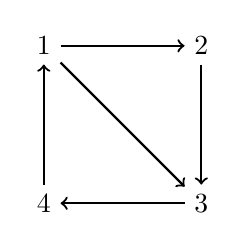
\begin{tikzpicture}
\node (atom1) at (0,2) {1};
\node (atom2) at (2,2) {2};
\node (atom3) at (2,0) {3};
\node (atom4) at (0,0) {4};
\draw[->, thick] (atom1)--(atom2);
\draw[->, thick] (atom2)--(atom3);
\draw[->, thick] (atom3)--(atom4);
\draw[->, thick] (atom4)--(atom1);
\draw[->, thick] (atom1) -- (atom3);
\end{tikzpicture}
\end{center}
This diagram could be used to describe an interpretation whose domain is the first four positive whole numbers, and which interprets `$\atom{R}{x,y}$' as being true of and only of:
	\begin{center}
		\ntuple{1, 2}, 
		\ntuple{2, 3}, 
		\ntuple{3, 4}, 
		\ntuple{4, 1}, 
		\ntuple{1, 3}
	\end{center}
Equally we might offer this diagram:

\begin{center}
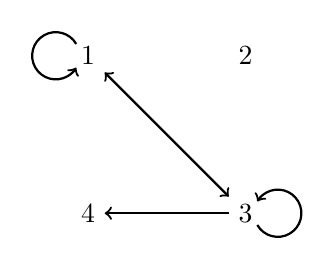
\begin{tikzpicture}
\node (atom1) at (0,2) {1};
\node (atom2) at (2,2) {2};
\node (atom3) at (2,0) {3};
\node (atom4) at (0,0) {4};
\draw[->, thick] (atom3)--(atom4);
\draw[->, thick] (atom1)+(-0.15,0.15) arc (-330:-30:.3); 
\draw[->, thick] (atom3)+(0.15,-0.15) arc (-150:150:.3); 
\draw[<->, thick] (atom1) -- (atom3);
\end{tikzpicture}
\end{center}
for an interpretation with the same domain, which takes the extension of `$\atom{R}{x,y}$' as:
	\begin{center}
		\ntuple{1, 3}, 
		\ntuple{3, 1}, 
		\ntuple{3, 4}, 
		\ntuple{1, 1},
		\ntuple{3, 3}
	\end{center}
If we wanted, we could make our diagrams more complex. For example, we could add names as labels for particular objects. Equally, to symbolize the extension of a one-place predicate, we might simply draw a ring around some particular objects and stipulate that the thus encircled objects (and only them) are to fall under the predicate `$\atom{H}{x}$', say. 


\chapter{Truth in FOL}\label{s:TruthFOL}
We have introduced you to interpretations. Since, among other things, they tell us which predicates are true of which objects, they will provide us with an account of the truth of atomic sentences. However, we now need to say, precisely, what it is for an arbitrary FOL sentence to be true or false in an interpretation. 

We know from \S\ref{s:FOLSentences} that there are three kinds of sentence in FOL: 
	\begin{ebullet}
		\item atomic sentences
		\item sentences whose main logical operator is a sentential connective
		\item sentences whose main logical operator is a quantifier
	\end{ebullet}
We need to explain truth for all three kinds of sentence.

We will provide a completely general explanation in this section. However, to try to keep the explanation comprehensible, we will, at several points, use the following interpretation:
	\begin{ekey}
		\item[\text{domain}] all people born before 2000\textsc{ce}
		\item[a] Aristotle
		\item[b] Beyonc\'e
		\item[\atom{P}{x}] \gap{x} is a philosopher
		\item[\atom{R}{x,y}] \gap{x} was born before \gap{y}
	\end{ekey}
This will be our \emph{go-to example} in what follows.

\section{Atomic sentences}
The truth of atomic sentences should be fairly straightforward. For sentence letters, the interpretation specifies if it is true or false. The sentence `$\atom{P}{a}$' should be true just in case `$\atom{P}{x}$' is true of `$a$'. Given our go-to interpretation, this is true iff Aristotle is a philosopher. Aristotle is a philosopher. So the sentence is true. Equally, `$\atom{P}{b}$' is false on our go-to interpretation.

Likewise, on this interpretation, `$\atom{R}{a,b}$' is true iff the object named by `$a$' was born before the object named by `$b$'. Well, Aristotle was born before Beyonc\'e. So `$\atom{R}{a,b}$' is true. Equally, `$\atom{R}{a,a}$' is false: Aristotle was not born before Aristotle. 

Dealing with atomic sentences, then, is very intuitive. When \metav{R} is an $n$-place predicate and $\metav{a}_1$, $\metav{a}_{2}$, \dots, $\metav{a}_{n}$ are names, 

	\factoidbox{
		The sentence $\atom{\metav{R}}{\metav{a}_{1},\metav{a}_{2},\dots,\metav{a}_{n}}$ is true in an interpretation \textbf{iff}\\
		$\metav{R}$ is true of the objects named by $\metav{a}_{1}$, $\metav{a}_{2}$, \dots, $\metav{a}_{n}$ (in that order) in that interpretation.
	}
Recall, though, that there is a special kind of atomic sentence: two names connected by an identity sign constitute an atomic sentence. This kind of atomic sentence is also easy to handle. Where \metav{a} and \metav{b} are any names, 
	\factoidbox{
		$\metav{a} = \metav{b}$ is true in an interpretation \textbf{iff}\\
		 \metav{a} and \metav{b} name the very same object in that interpretation
	}
So in our go-to interpretation, `$a = b$' is false, since Aristotle is distinct from Beyonc\'e.


\section{Sentential connectives}
We saw in \S\ref{s:FOLSentences} that FOL sentences can be built up from simpler ones using the truth-functional connectives that were familiar from TFL. The rules governing these truth-functional connectives are \emph{exactly} the same as they were when we considered TFL. Here they are:
	\factoidbox{
		$\metav{A} \eand \metav{B}$ is true in an interpretation \textbf{iff}\\ both $\metav{A}$ is true and $\metav{B}$ is true in that interpretation
		
		\medskip
		
		$\metav{A} \eor \metav{B}$ is true in an interpretation \textbf{iff}\\ either $\metav{A}$ is true or $\metav{B}$ is true in that interpretation

		\medskip
		$\enot \metav{A}$ is true in an interpretation \textbf{iff} \\$\metav{A}$ is false in that interpretation

		\medskip
		$\metav{A} \eif \metav{B}$ is true in an interpretation \textbf{iff}\\ either $\metav{A}$ is false or $\metav{B}$ is true in that interpretation

		\medskip
		$\metav{A} \eiff \metav{B}$ is true in an interpretation \textbf{iff} \\$\metav{A}$ has the same truth value as $\metav{B}$ in that interpretation
	}
This presents the very same information as the characteristic truth tables for the connectives; it just does so in a slightly different way. Some examples will probably help to illustrate the idea. (Make sure you understand them!) On our go-to interpretation:
	\begin{earg}
		\item[\textbullet] `$a = a \eand \atom{P}{a}$' is true
		\item[\textbullet] `$\atom{R}{a,b} \eand \atom{P}{b}$' is false because, although `$\atom{R}{a,b}$' is true, `$\atom{P}{b}$' is false
		\item[\textbullet] `$a = b \eor \atom{P}{a}$' is true
		\item[\textbullet] `$\enot a = b$' is true
		\item[\textbullet] `$\atom{P}{a} \eand \enot( a= b \eand \atom{R}{a,b})$' is true, because `$\atom{P}{a}$' is true and `$a = b$' is false
	\end{earg}
Make sure you understand these examples.

\section[Quantifiers]{When the main logical operator is a quantifier}\label{s:MainLogicalOperatorQuantifier}
The exciting innovation in FOL, though, is the use of \emph{quantifiers}, but expressing the truth conditions for quantified sentences is a bit more fiddly than one might first expect. 

Here is a na\"{i}ve first thought. We want to say that `$\forall x\, \atom{F}{x}$' is true iff `$\atom{F}{x}$' is true of everything in the domain. This should not be too problematic: our interpretation will specify directly what `$\atom{F}{x}$' is true of. 

Unfortunately, this na\"{i}ve thought is not general enough. For example, we want to be able to say that `$\forall x \exists y\, \atom{L}{x,y}$' is true just in case (speaking roughly) `$\exists y\, \atom{L}{x,y}$' is true of everything in the domain. But our interpretation does not \emph{directly} specify what `$\exists y\, \atom{L}{x,y}$' is true of. Instead, whether or not this is true of something should follow just from the interpretation of the predicate `$L$', the domain, and the meanings of the quantifiers. 

So here is a second na\"{i}ve thought. We might try to say that `$\forall x \exists y\, \atom{L}{x,y}$' is to be true in an interpretation iff $\exists y\, \atom{L}{\metav{a},y}$ is true for \emph{every} name \metav{a} that we have included in our interpretation. Similarly, we might try to say that $\exists y\, \atom{L}{\metav{a},y}$ is true just in case $\atom{L}{\metav{a},\metav{b}}$ is true for \emph{some} name \metav{b} that we have included in our interpretation.

Unfortunately, this is not right either. To see this, observe that our go-to interpretation only interprets \emph{two} names, `$a$' and `$b$'. But the domain---all people born before the year 2000\textsc{ce}---contains many more than two people. (And we have no intention of trying to correct for this by naming \emph{all} of them!)

So here is a third thought. (And this thought is not na\"{i}ve, but correct.) Although it is not the case that we have named \emph{everyone}, each person \emph{could} have been given a name. So we should focus on this possibility of extending an interpretation by adding a new name. We will offer a few examples of how this might work, centring on our go-to interpretation, and we will then present the formal definition. 

In our go-to interpretation, `$\exists x\, \atom{R}{b,x}$' should be true. After all, in the domain, there is certainly someone who was born after Beyonc\'e. Lady Gaga is one of those people. Indeed, if we were to extend our go-to interpretation---temporarily, mind---by adding the name `$c$' to refer to Lady Gaga, then `$\atom{R}{b,c}$' would be true on this extended interpretation. This, surely, should suffice to make `$\exists x\, \atom{R}{b,x}$' true on the original go-to interpretation. 

In our go-to interpretation, `$\exists x (\atom{P}{x} \eand \atom{R}{x,a})$' should also be true. After all, in the domain, there is certainly someone who was both a philosopher and born before Aristotle. Socrates is one such person. Indeed, if we were to extend our go-to interpretation by letting a new name, `$c$', denote Socrates, then `$\atom{W}{c} \eand \atom{R}{c,a}$' would be true on this extended interpretation. Again, this should surely suffice to make `$\exists x (\atom{P}{x} \eand \atom{R}{x,a})$' true on the original go-to interpretation. 

In our go-to interpretation, `$\forall x \exists y\, \atom{R}{x,y}$' should be false. After all, consider the last person born in the year 1999. We don't know who that was, but if we were to extend our go-to interpretation by letting a new name, `$d$', denote that person, then we would not be able to find anyone else in the domain to denote with some further new name, perhaps `$e$', in such a way that `$\atom{R}{d,e}$' would be true. Indeed, no matter \emph{whom} we named with `$e$', `$\atom{R}{d,e}$' would be false. This observation is surely sufficient to make `$\exists y\, \atom{R}{d,y}$' \emph{false} in our extended interpretation, which in turn is surely sufficient to make `$\forall x \exists y\, \atom{R}{x,y}$' false on the original go-to interpretation.

If you have understood these three examples, that's what matters. It provides the basis for a formal definition of truth for quantified sentences. 

Strictly speaking, though, we still need to \emph{give} that definition. The result, sadly, is a bit ugly, and requires a few new definitions. Brace yourself!

Suppose that \metav{A} is a formula containing at least one occurrence of the variable \metav{x}, and that $\metav{x}$ is free in $\metav{A}$. We will write this thus:
$$\metav{A}(\ldots \metav{x} \ldots \metav{x} \ldots)$$
Suppose also that \metav{c} is a name. Then we will write:
$$\metav{A}(\ldots \metav{c} \ldots \metav{c} \ldots)$$
for the formula we obtain by replacing \emph{every} occurrence of $\metav{x}$ in \metav{A} with~$\metav{c}$. The resulting formula is called a \define{substitution instance} of $\forall \metav{x}\metav{A}$ and $\exists\metav{x}\metav{A}$.  Also, $\metav{c}$ is called the \define{instantiating name}. So:
	$$\exists x (\atom{R}{e,x} \eiff \atom{F}{x})$$
is a substitution instance of 
	$$\forall y \exists x (\atom{R}{y,x} \eiff \atom{F}{x})$$
with the instantiating name `$e$' and instantiated variable~`$y$'.

\newglossaryentry{substitution instance}{
  name = substitution instance,
  description = {The result of replacing every free occurrence of a \gls{variable} in a \gls{formula} with a \gls{name}}
}

Our interpretation will include a specification of which names correspond to which objects in the domain. Take any object in the domain, say, $d$, and a name $\metav{c}$ which is not already assigned by the interpretation. If our interpretation is $\mathbf{I}$, then we can consider the interpretation $\mathbf{I}[d/\metav{c}]$ which is just like $\mathbf{I}$ except it \emph{also} assigns the name $\metav{c}$ to the object~$d$. Then we can say that $d$ \define{satisfies} the formula $\metav{A}(\dots\metav{x}\dots\metav{x}\dots)$ in the interpretation~$\mathbf{I}$ if, and only if, $\metav{A}(\dots\metav{c}\dots\metav{c}\dots)$ is true in $\mathbf{I}[d/\metav{c}]$. (If $d$ satisfies $\metav{A}(\dots\metav{x}\dots\metav{x}\dots)$ we also say that $\metav{A}(\dots\metav{x}\dots\metav{x}\dots)$ is \emph{true of}~$d$.) 

\factoidbox{The interpretation $\mathbf{I}[d/\metav{c}]$ is just like the interpretation $\mathbf{I}$ except it also assigns the name $\metav{c}$ to the object~$d$.

\
\\
An object $d$ \define{satisfies} $\metav{A}(\dots\metav{x}\dots\metav{x}\dots)$ in interpretation~$\mathbf{I}$ \textbf{iff} $\metav{A}(\dots\metav{c}\dots\metav{c}\dots)$ is true in $\mathbf{I}[d/\metav{c}]$.
}

So, for instance, Socrates satisfies the formula~$\atom{P}{x}$ since $\atom{P}{c}$ is true in the interpretation $\mathbf{I}[\text{Socrates}/c]$, i.e., the interpretation:
\begin{ekey}
	\item[\text{domain}] all people born before 2000\textsc{ce}
	\item[a] Aristotle
	\item[b] Beyonc\'e
	\item[c] Socrates 
	\item[\atom{P}{x}] \gap{x} is a philosopher
	\item[\atom{R}{x,y}] \gap{x} was born before \gap{y}
\end{ekey}

Armed with this notation, the rough idea is as follows. The sentence $\forall \metav{x}\metav{A}(\ldots \metav{x} \ldots \metav{x} \ldots)$ will be true in $\mathbf{I}$ iff, for any object~$d$ in the domain, $\metav{A}(\ldots \metav{c} \ldots \metav{c}\ldots)$ is true in $\mathbf{I}[d/\metav{c}]$, i.e., no matter what object (in the domain) we name with $\metav{c}$. In other words, $\forall \metav{x} \metav{A}(\ldots \metav{x} \ldots \metav{x} \ldots)$ is true iff every object in the domain satisfies $\metav{A}(\ldots \metav{x} \ldots \metav{x} \ldots)$. Similarly, the sentence $\exists \metav{x}\metav{A}$ will be true iff there is \emph{some} object that satisifes $\metav{A}(\ldots \metav{x} \ldots \metav{x} \ldots)$, i.e., $\metav{A}(\ldots \metav{c} \ldots \metav{c} \ldots)$ true in $\mathbf{I}[d/\metav{c}]$ for some object~$d$.
	\factoidbox{
		$\forall \metav{x}\metav{A}(\ldots \metav{x}\ldots\metav{x}\ldots)$ is true in an interpretation \textbf{iff}\\ 
		every object in the domain satisfies $\metav{A}(\ldots \metav{x} \ldots \metav{x}\ldots)$.
		
		\
		\\
		$\exists \metav{x}\metav{A}(\ldots \metav{x}\ldots\metav{x}\ldots)$ is true in an interpretation \textbf{iff}\\ at least one object in the domain satisfies
		$\metav{A}(\ldots \metav{x}\ldots\metav{x}\ldots)$.
	}
To be clear: all this is doing is formalizing (very pedantically) the intuitive idea expressed on the previous page. The result is a bit ugly, and the final definition might look a bit opaque. Hopefully, though, the \emph{spirit} of the idea is clear. 

Finally, let us note that the concept of an object satisfying a formula with a free variable can also be extended to formulas with more than one free variable. If we have a formula $\metav{A}(\metav{x},\metav{y})$ with two free variables $\metav{x}$ and $\metav{y}$, then we can say that a pair of objects $\langle a, b\rangle$ satisfies $\metav{A}(\metav{x},\metav{y})$ iff $\metav{A}(\metav{c},\metav{d})$ is true in the interpretation extended by two names $\metav{c}$ and $\metav{d}$, where $\metav{c}$ names~$a$ and $\metav{d}$ names~$b$. So, for instance, $\langle \text{Socrates}, \text{Plato}\rangle$ satisfies $R(x,y)$ since $R(c,d)$ is true in the interpretation:
\begin{ekey}
	\item[\text{domain}] all people born before 2000\textsc{ce}
	\item[a] Aristotle
	\item[b] Beyonc\'e
	\item[c] Socrates
	\item[d] Plato
	\item[\atom{P}{x}] \gap{x} is a philosopher
	\item[\atom{R}{x,y}] \gap{x} was born before \gap{y}
\end{ekey}
For atomic formulas, the objects, pairs of objects, etc., that satisfy them are exactly the extension of the predicate given in the interpretation. But the notion of satisfaction also applies to non-atomic formulas, e.g., the formula $\atom{P}{x} \land \atom{R}{x,b}$ is satisfied by all philosophers born before Beyonc\'e. It even applies to formulas involving quantifiers, e.g., $P(x) \eand \lnot\exists y(P(y) \land R(y,x))$ is satisfied by all people who are philosophers and for whom it is true that no philosopher was born before them---in other words, it is true of the first philosopher.


\practiceproblems
\solutions
\problempart
\label{pr.TorF1}
Consider the following interpretation:
	\begin{ebullet}
		\item The domain comprises only Corwin and Benedict
		\item `$\atom{A}{x}$' is to be true of both Corwin and Benedict
		\item `$\atom{B}{x}$' is to be true of Benedict only
		\item `$\atom{N}{x}$' is to be true of no one
		\item `$c$' is to refer to Corwin
	\end{ebullet}
Determine whether each of the following sentences is true or false in that interpretation:
\begin{earg}
\item $\atom{B}{c} $
\item $\atom{A}{c}  \eiff \enot \atom{N}{c}$
\item $\atom{N}{c}  \eif (\atom{A}{c} \eor \atom{B}{c})$
\item $\forall x\, \atom{A}{x}$
\item $\forall x \enot \atom{B}{x}$
\item $\exists x(\atom{A}{x} \eand \atom{B}{x})$
\item $\exists x(\atom{A}{x} \eif \atom{N}{x})$
\item $\forall x(\atom{N}{x} \eor \enot \atom{N}{x})$
\item $\exists x\, \atom{B}{x} \eif \forall x\, \atom{A}{x}$
\end{earg}

\problempart
\label{pr.TorF2}
Consider the following interpretation:	
	\begin{ebullet}
		\item The domain comprises only Lemmy, Courtney and Eddy
		\item `$\atom{G}{x}$' is to be true of Lemmy, Courtney and Eddy.
		\item `$\atom{H}{x}$' is to be true of and only of Courtney
		\item `$\atom{M}{x}$' is to be true of and only of Lemmy and Eddy
		\item `$c$' is to refer to Courtney
		\item `$e$' is to refer to Eddy
	\end{ebullet}
Determine whether each of the following sentences is true or false in that interpretation:
\begin{earg}
\item $\atom{H}{c} $
\item $\atom{H}{e} $
\item $\atom{M}{c}  \eor \atom{M}{e}$
\item $\atom{G}{c}  \eor \enot \atom{G}{c}$
\item $\atom{M}{c}  \eif \atom{G}{c}$
\item $\exists x\, \atom{H}{x}$
\item $\forall x\, \atom{H}{x}$
\item $\exists x\, \enot \atom{M}{x}$
\item $\exists x(\atom{H}{x} \eand \atom{G}{x})$
\item $\exists x(\atom{M}{x} \eand \atom{G}{x})$
\item $\forall x(\atom{H}{x} \eor \atom{M}{x})$
\item $\exists x\, \atom{H}{x} \eand \exists x\, \atom{M}{x}$
\item $\forall x(\atom{H}{x} \eiff \enot \atom{M}{x})$
\item $\exists x\, \atom{G}{x} \eand \exists x \enot \atom{G}{x}$
\item $\forall x\exists y(\atom{G}{x} \eand \atom{H}{y})$
\end{earg}

\problempart
\label{pr.TorF3}
Following the diagram conventions introduced at the end of \S\ref{s:Interpretations}, consider the following interpretation:	
\begin{center}
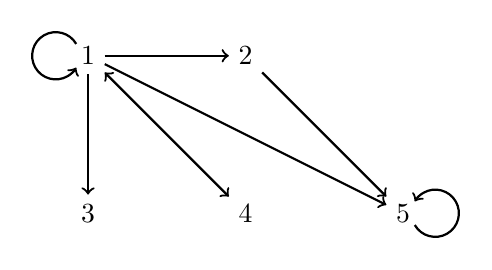
\begin{tikzpicture}
\node (atom1) at (0,2) {1};
\node (atom2) at (2,2) {2};
\node (atom4) at (0,0) {3};
\node (atom5) at (2,0) {4};
\node (atom6) at (4,0) {5};
\draw[->, thick] (atom1)+(-0.15,0.15) arc (-330:-30:.3); 
\draw[->, thick] (atom6)+(0.15,-0.15) arc (-150:150:.3); 
\draw[->, thick] (atom1) -- (atom2);
\draw[->, thick] (atom1) -- (atom4);
\draw[<->, thick] (atom1) -- (atom5);
\draw[->, thick] (atom1) -- (atom6);
\draw[->, thick] (atom2) -- (atom6);
\end{tikzpicture}
\end{center}
Determine whether each of the following sentences is true or false in that interpretation:
\begin{earg}
\item $\exists x\, \atom{R}{x,x}$
\item $\forall x\, \atom{R}{x,x}$
\item $\exists x \forall y\, \atom{R}{x,y}$
\item $\exists x \forall y\, \atom{R}{y,x}$
\item $\forall x \forall y \forall z ((\atom{R}{x,y} \eand \atom{R}{y,z}) \eif \atom{R}{x,z})$
\item $\forall x \forall y \forall z ((\atom{R}{x,y} \eand \atom{R}{x,z}) \eif \atom{R}{y,z})$
\item $\exists x \forall y\, \enot \atom{R}{x,y}$
\item $\forall x(\exists y\, \atom{R}{x,y} \eif \exists y\, \atom{R}{y,x})$
\item $\exists x \exists y (\enot x = y \eand \atom{R}{x,y} \eand \atom{R}{y,x})$
\item $\exists x \forall y(\atom{R}{x,y} \eiff x = y)$
\item $\exists x \forall y(\atom{R}{y,x} \eiff x = y)$
\item $\exists x \exists y(\enot x = y \eand \atom{R}{x,y} \eand \forall z(\atom{R}{z,x} \eiff y = z))$
\end{earg}


\chapter{Semantic concepts}

Defining truth in FOL was quite fiddly. But now that we are done, we can define various other central logical notions. These definitions will look very similar to those for TFL, from \S\ref{s:SemanticConcepts}. However, remember that they concern \emph{interpretations}, rather than valuations. 

We will use the symbol `$\entails$' for FOL much as we did for TFL. So:
	$$\metav{A}_1, \metav{A}_2, \ldots, \metav{A}_n \entails\metav{C}$$
means that there is no interpretation in which all of $\metav{A}_1$, $\metav{A}_2$, \dots, $\metav{A}_n$ are true and in which \metav{C} is false. Derivatively,
	$$\entails\metav{A}$$
means that \metav{A} is true in every interpretation.

The other logical notions also have corresponding definitions in FOL:

\begin{itemize}
\item An FOL sentence $\metav{A}$ is a \define{validity} iff $\metav{A}$ is true in every interpretation; i.e.,  $\entails\metav{A}$.
\newglossaryentry{validity}
{
name=validity,
description={A \gls{sentence of FOL} that is true in every \gls{interpretation}}
}

\item $\metav{A}$ is a \define{contradiction} iff $\metav{A}$ is false in every interpretation; i.e., $\entails\enot\metav{A}$.
\newglossaryentry{contradiction of FOL}
{
  name=contradiction (of FOL),
  text=contradiction,
description={A \gls{sentence of FOL} that is false in every \gls{interpretation}}
}
  
\item $\metav{A}_1, \metav{A}_2, \ldots \metav{A}_n \therefore \metav{C}$ is \define{valid in FOL} iff there is no interpretation in which all of the premises are true and the conclusion is false; i.e., $\metav{A}_1,\metav{A}_2,\ldots \metav{A}_n \entails\metav{C}$. It is \define{invalid in FOL} otherwise.
\newglossaryentry{valid in FOL}
{
  name=validity of arguments (in FOL),
  text = valid,
description={A property held by arguments; an argument is valid if and only if no \gls{interpretation} makes all premises true and the conclusion false}
}

\item Two FOL sentences \metav{A} and \metav{B} are \define{equivalent} iff they are true in exactly the same interpretations as each other; i.e., both $\metav{A}\entails\metav{B}$ and $\metav{B}\entails\metav{A}$.

\newglossaryentry{equivalent in FOL}
{
  name=equivalence (in FOL),
  text = equivalent,
description={A property held by pairs of \glspl{sentence of FOL} if and only if the sentences have the same truth value in every \gls{interpretation}}
}

\item The FOL sentences $\metav{A}_1$, $\metav{A}_2$, \dots, $\metav{A}_n$ are \define{jointly satisfiable} iff some interpretation makes all of them true. They are \define{jointly unsatisfiable} iff there is no such interpretation.
\newglossaryentry{satisfiable in FOL}
{
  name=satisfiability (in FOL),
  text=jointly satisfiable,
description={A property held by \glspl{sentence of FOL} if and only if some \gls{interpretation} makes all the sentences true}
}
\end{itemize}

\chapter{Using interpretations}
\label{sec.UsingModels}

\section{Validities and contradictions}
Suppose we want to show that `$\exists x\, \atom{A}{x,x} \eif \atom{B}{d}$' is \emph{not} a validity. This requires showing that the sentence is not true in every interpretation; i.e.,\ that it is false in some interpretation. If we can provide just one interpretation in which the sentence is false, then we will have shown that the sentence is not a validity.

In order for `$\exists x\,\atom{A}{x,x} \eif \atom{B}{d}$' to be false, the antecedent (`$\exists x\, \atom{A}{x,x}$') must be true, and the consequent (`$\atom{B}{d}$') must be false. To construct such an interpretation, we start by specifying a domain. Keeping the domain small makes it easier to specify what the predicates will be true of, so we will start with a domain that has just one member. For concreteness, let's say it is \emph{just} the city of Paris. 
	\begin{ekey}
		\item[\text{domain}] Paris
	\end{ekey}
The name `$d$' must refer to something in the domain, so we have no option but:
	\begin{ekey}
		\item[d] Paris
	\end{ekey}
Recall that we want `$\exists x\, \atom{A}{x,x}$' to be true, so we want all members of the domain to be paired with themselves in the extension of `$A$'. We can just offer:
	\begin{ekey}
		\item[\atom{A}{x,y}] \gap{x} is identical with \gap{y}
	\end{ekey}
Now `$\atom{A}{d,d}$' is true, so it is surely true that `$\exists x\, \atom{A}{x,x}$'. Next, we want `$\atom{B}{d}$' to be false, so the referent of `$d$' must not be in the extension of `$B$'. We might simply offer:
	\begin{ekey}
		\item[\atom{B}{x}] \gap{x} is in Germany
	\end{ekey}
Now we have an interpretation where `$\exists x\, \atom{A}{x,x}$' is true, but where `$\atom{B}{d}$' is false. So there is an interpretation where `$\exists x\, \atom{A}{x,x} \eif \atom{B}{d}$' is false. So `$\exists x\, \atom{A}{x,x} \eif \atom{B}{d}$' is not a validity.

We can just as easily show that `$\exists x\atom{A}{x,x} \eif \atom{B}{d}$' is not a contradiction. We need only specify an interpretation in which `$\exists x\atom{A}{x,x} \eif \atom{B}{d}$' is true; i.e., an interpretation in which either `$\exists x\, \atom{A}{x,x}$' is false or `$\atom{B}{d}$' is true. Here is one:
	\begin{ekey}
		\item[\text{domain}] Paris
		\item[d] Paris
		\item[\atom{A}{x,y}] \gap{x} is identical with \gap{y}
		\item[\atom{B}{x}] \gap{x} is in France
	\end{ekey}
This shows that there is an interpretation where `$\exists x\atom{A}{x,x} \eif \atom{B}{d}$' is true. So `$\exists x\, \atom{A}{x,x} \eif \atom{B}{d}$' is not a contradiction.
	\factoidbox{
		To show that $\metav{A}$ is not a validity, it suffices to find an interpretation where $\metav{A}$ is false.
		
		To show that $\metav{A}$ is not a contradiction, it suffices to find an interpretation where $\metav{A}$ is true.
	}

\section{Logical equivalence}
Suppose we want to show that `$\forall x\, \atom{S}{x}$' and `$\exists x\, \atom{S}{x}$' are not logically equivalent. We need to construct an interpretation in which the two sentences have different truth values; we want one of them to be true and the other to be false. We start by specifying a domain. Again, we make the domain small so that we can specify extensions easily. In this case, we will need at least two objects. (If we chose a domain with only one member, the two sentences would end up with the same truth value. In order to see why, try constructing some partial interpretations with one-member domains.) For concreteness, let's take:
	\begin{ekey}
		\item[\text{domain}] Ornette Coleman, Miles Davis
	\end{ekey}
We can make `$\exists x\, \atom{S}{x}$' true by including something in the extension of `$S$', and we can make `$\forall x\, \atom{S}{x}$' false by leaving something out of the extension of `$S$'. For concreteness, let's say:
	\begin{ekey}
		\item[\atom{S}{x}] \gap{x} plays saxophone
	\end{ekey}
Now `$\exists x\, \atom{S}{x}$' is true, because `$\atom{S}{x}$' is true of Ornette Coleman. Slightly more precisely, extend our interpretation by allowing `$c$' to name Ornette Coleman.  `$\atom{S}{c}$' is true in this extended interpretation, so `$\exists x\, \atom{S}{x}$' was true in the original interpretation. Similarly, `$\forall x\, \atom{S}{x}$' is false, because `$\atom{S}{x}$' is false of Miles Davis. Slightly more precisely, extend our interpretation by allowing `$d$' to name Miles Davis, and `$\atom{S}{d}$' is false in this extended interpretation, so `$\forall x\, \atom{S}{x}$' was false in the original interpretation. We have provided a counter-interpretation to the claim that `$\forall x\, \atom{S}{x}$' and `$\exists x\, \atom{S}{x}$' are logically equivalent.
	\factoidbox{
		To show that $\metav{A}$ and $\metav{B}$ are not logically equivalent, it suffices to find an interpretation where one is true and the other is false.
	}

\section{Validity, entailment and satisfiability}
To test for validity, entailment, or satisfiability, we typically need to produce interpretations that determine the truth value of several sentences simultaneously. 

Consider the following argument in FOL:
$$\exists x(\atom{G}{x} \eif \atom{G}{a}) \therefore \exists x\, \atom{G}{x} \eif \atom{G}{a}$$
To show that this is invalid, we must make the premise true and the conclusion false. The conclusion is a conditional, so to make it false, the antecedent must be true and the consequent must be false. Clearly, our domain must contain two objects. Let's try:
	\begin{ekey}
		\item[\text{domain}] Karl Marx, Ludwig von Mises
		\item[\atom{G}{x}] \gap{x} hated communism
		\item[a] Karl Marx
	\end{ekey}
Given that Marx wrote \emph{The Communist Manifesto}, `$\atom{G}{a}$' is plainly false in this interpretation. But von Mises famously hated communism, so `$\exists x\, \atom{G}{x}$' is true in this interpretation. Hence `$\exists x\, \atom{G}{x} \eif \atom{G}{a}$' is false, as required. 

Does this interpretation make the premise true? Yes it does! Note that `$\atom{G}{a} \eif \atom{G}{a}$' is true. (Indeed, it is a validity.) But then certainly `$\exists x (\atom{G}{x} \eif \atom{G}{a})$' is true, so the premise is true, and the conclusion is false, in this interpretation. The argument is therefore invalid. 

In passing, note that we have also shown that `$\exists x(\atom{G}{x} \eif \atom{G}{a})$' does \emph{not} entail `$\exists x\, \atom{G}{x} \eif \atom{G}{a}$', i.e., that $\exists x (\atom{G}{x} \eif \atom{G}{a}) \nentails \exists x \atom{G}{x} \eif \atom{G}{a}$. Equally, we have shown that the sentences `$\exists x (\atom{G}{x} \eif \atom{G}{a})$' and `$\enot (\exists x\, \atom{G}{x} \eif \atom{G}{a})$' are jointly satisfiable.

Let's consider a second example. Consider:
$$\forall x \exists y\, \atom{L}{x,y} \therefore \exists y \forall x\, \atom{L}{x,y}$$
Again, we want to show that this is invalid. To do this, we must make the premises true and the conclusion false. Here is a suggestion:
\begin{ekey}
	\item[\text{domain}] Canadian citizens currently in a domestic partnership with another Canadian citizen
	\item[\atom{L}{x,y}] \gap{x} is in a domestic partnership with \gap{y}
\end{ekey}
The premise is clearly true on this interpretation. Anyone in the domain is a Canadian citizen in a domestic partnership with some other Canadian citizen. That other citizen will also, then, be in the domain. So for everyone in the domain, there will be someone (else) in the domain with whom they are in a domestic partnership. Hence `$\forall x \exists y\, \atom{L}{x,y}$' is true. However, the conclusion is clearly false, for that would require that there is some single person who is in a domestic partnership with everyone in the domain, and there is no such person, so the argument is invalid. We observe immediately that the sentences `$\forall x \exists y\, \atom{L}{x,y}$' and `$\enot\exists y \forall x\, \atom{L}{x,y}$' are jointly satisfiable and that `$\forall x \exists y\, \atom{L}{x,y}$' does not entail `$\exists y \forall x\, \atom{L}{x,y}$'. 

For our third example, we'll mix things up a bit. In \S\ref{s:Interpretations}, we described how we can present some interpretations using diagrams. For example:
\begin{center}
	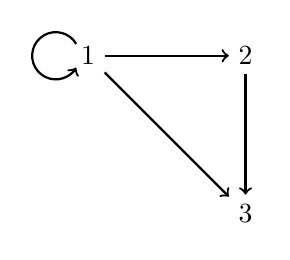
\begin{tikzpicture}
	\node (atom1) at (0,2) {1};
	\node (atom2) at (2,2) {2};
	\node (atom3) at (2,0) {3};
	\draw[->, thick] (atom1)--(atom2);
	\draw[->, thick] (atom1)--(atom3);
	\draw[->, thick] (atom1)+(-0.15,0.15) arc (-330:-30:.3); 
	\draw[->, thick] (atom2) -- (atom3);
	\end{tikzpicture}
\end{center}
Using the conventions employed in \S\ref{s:Interpretations}, the domain of this interpretation is the first three positive whole numbers, and `$\atom{R}{x,y}$' is true of x and y just in case there is an arrow from x to y in our diagram. Here are some sentences that the interpretation makes true:
\begin{ebullet}
	\item `$\forall x \exists y\, \atom{R}{y,x}$' 
	\item `$\exists x \forall y\, \atom{R}{x,y}$' \hfill witness 1
	\item `$\exists x \forall y (\atom{R}{y,x} \eiff x = y)$' \hfill witness 1
	\item `$\exists x \exists y \exists z ((\enot y = z \eand \atom{R}{x,y}) \eand \atom{R}{z,x})$' \hfill witness 2
	\item `$\exists x \forall y\, \enot \atom{R}{x,y}$' \hfill witness 3
	\item `$\exists x (\exists y\, \atom{R}{y,x} \eand \enot \exists y\, \atom{R}{x,y})$' \hfill witness 3
\end{ebullet}
This immediately shows that all of the preceding six sentences are jointly satisfiable. We can use this observation to generate \emph{invalid} arguments, e.g.:
\begin{align*}
	\forall x \exists y\, \atom{R}{y,x}, \exists x \forall y\, \atom{R}{x,y}  &\therefore  \forall x \exists y\, \atom{R}{x,y}\\
	\exists x \forall y\, \atom{R}{x,y}, \exists x \forall y \enot \atom{R}{x,y} & \therefore \enot \exists x \exists y \exists z (\enot y = z \eand (\atom{R}{x,y} \eand \atom{R}{z,x}))
\end{align*}
and many more besides.

\factoidbox{
	If some interpretation makes all of $\metav{A}_1, \metav{A}_2, \ldots, \metav{A}_n$  true and $\metav{C}$ is false, then:
	\begin{ebullet}
		\item$\metav{A}_1, \metav{A}_2, \ldots, \metav{A}_n \therefore \metav{C}$ is \emph{invalid}; and
	\item $\metav{A}_1, \metav{A}_2, \ldots, \metav{A}_n \nentails \metav{C}$; and
	\item 
	And $\metav{A}_1, \metav{A}_2, \ldots, \metav{A}_n, \enot \metav{C}$ are jointly consistent.
\end{ebullet}}
An interpretation which refutes a claim---to logical truth, say, or to entailment---is called a \emph{counter-interpretation}, or a \emph{counter-model}. 

We'll close this section, though, with a caution about the relationship between (in)validity and (non)entailment. Recall FOL's limitations: it is is an extensional language; it ignores issues of vagueness; and it cannot handle cases of validity for `special reasons'. To take one illustration of these issues, consider this natural-language argument: 
\begin{earg}
	\item[] Every fox is cute.
	\item[\therefore] All vixens are cute.
\end{earg}
This is valid: necessarily every vixen is a fox, so it is impossible for the premise to be true and the conclusion false. Now, we might sensibly symbolize the argument as follows:
$$\forall x(\atom{F}{x} \eif \atom{C}{x}) \therefore \forall x(\atom{V}{x} \eif  \atom{C}{x})$$
However, it is easy to find counter-models which show that $\forall x(\atom{F}{x} \eif \atom{C}{x}) \nentails \forall x(\atom{V}{x} \eif  \atom{C}{x})$. (\emph{Exercise}: find one.) So, it would be \emph{wrong} to infer that the English argument is \emph{invalid}, just because there is a counter-model to the relevant \emph{FOL-entailment}. 

The general moral is this. If you want to infer from the absence of an entailment in FOL to the invalidity of some English argument, then you need to argue that nothing important is lost in the way you have symbolized the English argument. 

\practiceproblems

\solutions
\problempart
\label{pr.Contingent}
Show that each of the following is neither a validity nor a contradiction:
\begin{earg}
\item \leftsolutions\ $\atom{D}{a}  \eand \atom{D}{b}$
\item \leftsolutions\ $\exists x\, \atom{T}{x,h}$
\item \leftsolutions\ $\atom{P}{m}  \eand \enot\forall x\, \atom{P}{x}$
\item $\forall z \atom{J}{z} \eiff \exists y\, \atom{J}{y}$
\item $\forall x (\atom{W}{x,m,n} \eor \exists y\atom{L}{x,y})$
\item $\exists x (\atom{G}{x} \eif \forall y\, \atom{M}{y})$
\item $\exists x (x = h \eand x = i)$
\end{earg}

\solutions
\problempart
\label{pr.NotEquiv}
Show that the following pairs of sentences are not logically equivalent.
\begin{earg}
\item $\atom{J}{a} $,  $\atom{K}{a}$
\item $\exists x\, \atom{J}{x}$,  $\atom{J}{m}$
\item $\forall x\, \atom{R}{x,x}$, $\exists x\, \atom{R}{x,x}$
\item $\exists x\, \atom{P}{x} \eif \atom{Q}{c}$, $\exists x (\atom{P}{x} \eif \atom{Q}{c})$
\item $\forall x(\atom{P}{x} \eif \enot \atom{Q}{x})$, $\exists x(\atom{P}{x} \eand \enot \atom{Q}{x})$
\item $\exists x(\atom{P}{x} \eand \atom{Q}{x})$, $\exists x(\atom{P}{x} \eif \atom{Q}{x})$
\item $\forall x(\atom{P}{x}\eif \atom{Q}{x})$, $\forall x(\atom{P}{x} \eand \atom{Q}{x})$
\item $\forall x\exists y\, \atom{R}{x,y}$, $\exists x\forall y\, \atom{R}{x,y}$
\item $\forall x\exists y\, \atom{R}{x,y}$, $\forall x\exists y\, \atom{R}{y,x}$
\end{earg}



\problempart
Show that the following sentences are jointly satisfiable:
\begin{earg}
\item  $\atom{M}{a}, \enot \atom{N}{a}, \atom{P}{a}, \enot \atom{Q}{a}$
\item $\atom{L}{e,e}, \atom{L}{e,g}, \enot \atom{L}{g,e}, \enot \atom{L}{g,g}$
\item $\enot (\atom{M}{a} \eand \exists x\, \atom{A}{x}), \atom{M}{a} \eor \atom{F}{a}, \forall x(\atom{F}{x} \eif \atom{A}{x})$
\item $\atom{M}{a} \eor \atom{M}{b}, \atom{M}{a} \eif \forall x \enot \atom{M}{x}$
\item $\forall y\, \atom{G}{y}, \forall x (\atom{G}{x} \eif \atom{H}{x}), \exists y \enot \atom{I}{y}$
\item $\exists x(\atom{B}{x} \eor \atom{A}{x}), \forall x \enot \atom{C}{x}, \forall x\bigl[(\atom{A}{x} \eand \atom{B}{x}) \eif \atom{C}{x}\bigr]$
\item $\exists x\, \atom{X}{x}, \exists x\, \atom{Y}{x}, \forall x(\atom{X}{x} \eiff \enot \atom{Y}{x})$
\item $\forall x(\atom{P}{x} \eor \atom{Q}{x}), \exists x\enot(\atom{Q}{x} \eand \atom{P}{x})$
\item $\exists z(\atom{N}{z} \eand \atom{O}{z,z}), \forall x\forall y(\atom{O}{x,y} \eif \atom{O}{y,x})$
\item $\enot \exists x \forall y\, \atom{R}{x,y}, \forall x \exists y\, \atom{R}{x,y}$
\item $\enot \atom{R}{a,a}$, $\forall x (x=a \eor \atom{R}{x,a})$
\item $\forall x\forall y\forall z[(x=y \eor y=z )\eor x=z]$, $\exists x\exists y\ \enot x= y$
\item $\exists x\exists y((\atom{Z}{x} \eand \atom{Z}{y} )\eand x=y)$, $\enot \atom{Z}{d}$, $d=e$
\end{earg}

\problempart
Show that the following arguments are invalid:
\begin{earg}
\item $\forall x(\atom{A}{x} \eif \atom{B}{x}) \therefore \exists x\, \atom{B}{x}$
\item $\forall x(\atom{R}{x} \eif \atom{D}{x}), \forall x(\atom{R}{x} \eif \atom{F}{x}) \therefore \exists x(\atom{D}{x} \eand \atom{F}{x})$
\item $\exists x(\atom{P}{x}\eif \atom{Q}{x}) \therefore \exists x\, \atom{P}{x}$
\item $\atom{N}{a} \eand \atom{N}{b} \eand \atom{N}{c} \therefore \forall x\, \atom{N}{x}$
\item $\atom{R}{d,e}, \exists x\, \atom{R}{x,d} \therefore \atom{R}{e,d}$
\item $\exists x(\atom{E}{x} \eand \atom{F}{x}), \exists x\, \atom{F}{x} \eif \exists x\, \atom{G}{x} \therefore \exists x(\atom{E}{x} \eand \atom{G}{x})$
\item $\forall x\, \atom{O}{x,c}, \forall x\, \atom{O}{c,x} \therefore \forall x\, \atom{O}{x,x}$
\item $\exists x(\atom{J}{x} \eand \atom{K}{x}), \exists x \enot \atom{K}{x}, \exists x \enot \atom{J}{x} \therefore \exists x(\enot \atom{J}{x} \eand \enot \atom{K}{x})$
\item $\atom{L}{a,b} \eif \forall x\, \atom{L}{x,b}, \exists x\, \atom{L}{x,b} \therefore \atom{L}{b,b}$
\item $\forall x(\atom{D}{x} \eif \exists y\, \atom{T}{y,x}) \therefore \exists y \exists z\ \enot y= z$
\end{earg}

\chapter[Reasoning about interpretations]{Reasoning about all interpretations}

\section{Validities and contradictions}
We can show that a sentence is \emph{not} a validity just by providing one carefully specified interpretation: an interpretation in which the sentence is false. To show that something \emph{is} a validity, on the other hand, it would not be enough to construct ten, one hundred, or even a thousand interpretations in which the sentence is true. A sentence is only a validity if it is true in \emph{every} interpretation, and there are infinitely many interpretations. We need to reason about all of them, and we cannot do this by dealing with them one by one!

Sometimes, we can reason about all interpretations fairly easily. For example, we can offer a relatively simple argument that `$\atom{R}{a,a}\eor\enot \atom{R}{a,a}$' is a validity:
	\begin{quote}
		\label{allmodels1}
		Any relevant interpretation will give `$\atom{R}{a,a}$' a truth value. If `$\atom{R}{a,a}$' is true in an interpretation, then `$\atom{R}{a,a} \eor \enot\atom{R}{a,a}$' is true in that interpretation. If `$\atom{R}{a,a}$' is false in an interpretation, then $\enot\atom{R}{a,a}$ is true, and so `$\atom{R}{a,a} \eor\enot \atom{R}{a,a}$' is true in that interpretation. These are the only alternatives. So `$\atom{R}{a,a} \eor\enot \atom{R}{a,a}$' is true in every interpretation. Therefore, it is a validity.
	\end{quote}
This argument is valid, of course, and its conclusion is true. However, it is not an argument in FOL. Rather, it is an argument in English \emph{about} FOL: it is an argument in the metalanguage. 

Note another feature of the argument. Since the sentence in question contained no quantifiers, we did not need to think about how to interpret `$a$' and `$R$'; the point was just that, however we interpreted them, `$\atom{R}{a,a}$' would have some truth value or other. (We could ultimately have given the same argument concerning TFL sentences.)

Let's have another example. The sentence `$\forall x(\atom{R}{x,x}\eor\enot \atom{R}{x,x})$' should obviously be a validity. However, saying \emph{precisely} why is quite tricky. We cannot say that `$\atom{R}{x,x} \eor\enot \atom{R}{x,x}$' is true in every interpretation, since `$\atom{R}{x,x} \eor\enot \atom{R}{x,x}$' is not even a \emph{sentence} of FOL (remember that `$x$' is a variable, not a name). Instead, we should say something like this:
	\begin{quote}
		Consider some arbitrary interpretation. $\forall x(\atom{R}{x,x}\eor \enot\atom{R}{x,x})$ is true in our interpretation iff $\atom{R}{x,x}\eor\enot\atom{R}{x,x}$ is satisfied by every object of its domain. Consider some arbitrary member of the domain, which, for convenience, we will call Fred. Either Fred satisfies $\atom{R}{x,x}$ or it does not. If Fred satisfies `$\atom{R}{x,x}$', then Fred also satisfies `$\atom{R}{x,x} \eor \enot \atom{R}{x,x}$'. If Fred does not satisfy `$\atom{R}{x,x}$', it \emph{does} satisfy `$\enot\atom{R}{x,x}$' and so also `$\atom{R}{x,x} \eor\enot \atom{R}{x,x}$'.\footnote{We use here the fact that the truth conditions for connectives also apply to satisfaction: $a$ satisfies $\metav{A}(\metav{x}) \lor \metav{B}(\metav{x})$ iff $a$ satisfies $\metav{A}(\metav{x})$ or $\metav{B}(\metav{x})$, etc.} So either way, Fred satisfies `$\atom{R}{x,x} \eor\enot \atom{R}{x,x}$'. Since there was nothing special about Fred---we might have chosen any object---we see that every object in the domain satisfies `$\atom{R}{x,x} \eor\enot \atom{R}{x,x}$'. So `$\forall x (\atom{R}{x,x} \eor\enot \atom{R}{x,x})$' is true in our interpretation. But we chose our interpretation arbitrarily, so `$\forall x (\atom{R}{x,x} \eor\enot \atom{R}{x,x})$' is true in every interpretation. It is therefore a validity.
	\end{quote}
This is quite longwinded, but, as things stand, there is no alternative. In order to show that a sentence is a validity, we must reason about \emph{all} interpretations. 

\section{Other cases}
Similar points hold of other cases too. Thus, we must reason about all interpretations if we want to show:
	\begin{ebullet}
		\item that a sentence is a contradiction; for this requires that it is false in \emph{every} interpretation. 
		\item that two sentences are logically equivalent; for this requires that they have the same truth value in \emph{every} interpretation.
		\item that some sentences are jointly unsatisfiable; for this requires that there is no interpretation in which all of those sentences are true together; i.e.\ that, in \emph{every} interpretation, at  least one of those sentences is false.
		\item that an argument is valid; for this requires that the conclusion is true in \emph{every} interpretation where the premises are true. 
		\item that some sentences entail another sentence.
	\end{ebullet}
The problem is that, with the tools available to you so far, reasoning about all interpretations is a serious challenge! For a final example, here is a perfectly obvious entailment:
	$$\forall x(\atom{H}{x} \eand \atom{J}{x}) \entails \forall x\, \atom{H}{x}$$
After all, if everything is both $H$ and $J$, then everything is~$H$. But we can only establish the entailment by considering what must be true in every interpretation in which the premise is true. To show this, we would have to reason as follows:
	\begin{quote}
		Consider an arbitrary interpretation in which `$\forall x(\atom{H}{x} \eand \atom{J}{x})$' is true. It follows that `$\atom{H}{x} \eand \atom{J}{x}$' is satisfied by every object in this interpretation. `$\atom{H}{x}$' will, then, also be satisfied by every object.\footnote{Here again we make use of the fact that any object that satisfies $\metav{A}(\metav{x}) \land \metav{B}(\metav{x})$ must satisfy both $\metav{A}(\metav{x})$ and $\metav{B}(\metav{x})$.} So it must be that `$\forall x\, \atom{H}{x}$' is true in the  interpretation. We've assumed nothing about the interpretation except that it was one in which `$\forall x(\atom{H}{x} \eand \atom{J}{x})$' is true. So any interpretation in which `$\forall x(\atom{H}{x} \eand \atom{J}{x})$' is true is one in which `$\forall x\, \atom{H}{x}$' is true.
\end{quote}
Even for a simple entailment like this one, the reasoning is somewhat complicated. For more complicated entailments, the reasoning can be extremely torturous.

The following table summarises whether a single interpretation or counter-interpretation suffices, or whether we must reason about all interpretations.

\begin{center}\small
\begin{tabular}{l l l}
%\cline{2-3}
 & \textbf{Yes} & \textbf{No}\\
 \hline
%\cline{2-3}
validity? & all interpretations & one counter-interpretation\\
contradiction? &  all interpretations  & one counter-interpretation\\
equivalent? & all interpretations & one counter-interpretation\\
satisfiable? & one interpretation & all interpretations\\
valid? & all interpretations & one counter-interpretation\\
entailment? & all interpretations & one counter-interpretation\\
\end{tabular}
\end{center}
\label{table.ModelOrArgument}

You might want to compare this table with the table at the end of \S\ref{s:PartialTruthTable}. The key difference resides in the fact that TFL concerns truth tables, whereas FOL concerns interpretations. This difference is deeply important, since each truth-table only ever has finitely many lines, so that a complete truth table is a relatively tractable object. By contrast, there are infinitely many interpretations for any given sentence(s), so that reasoning about all interpretations can be a deeply tricky business. 

%!TEX root = forallxyyc.tex
\part{Natural deduction for FOL}
\label{ch.NDFOL}
\addtocontents{toc}{\protect\mbox{}\protect\hrulefill\par}

\chapter{Basic rules for FOL}\label{s:BasicFOL}

The language of FOL makes use of all of the connectives of TFL. So proofs in FOL will use all of the basic and derived rules from Part~\ref{ch.NDTFL}. We will also use the proof-theoretic notions (particularly, the symbol `$\proves$') introduced there. However, we will also need some new basic rules to govern the quantifiers, and to govern the identity sign.


\section{Universal elimination}

From the claim that everything is~$F$, you can infer that any particular thing is~$F$. You name it; it's~$F$. So the following should be fine:
\begin{fitchproof}
	\hypo{a}{\forall x\,\atom{R}{x,x,d}}
	\have{c}{\atom{R}{a,a,d}} \Ae{a}
\end{fitchproof}
We obtained line 2 by dropping the universal quantifier and replacing every instance of `$x$' with `$a$'. Equally, the following should be allowed:
\begin{fitchproof}
	\hypo{a}{\forall x\,\atom{R}{x,x,d}}
	\have{c}{\atom{R}{d,d,d}} \Ae{a}
\end{fitchproof}
We obtained line 2 here by dropping the universal quantifier and replacing every instance of `$x$' with `$d$'. We could have done the same with any other name we wanted. 

This motivates the universal elimination rule ($\forall$E):
\factoidbox{
\begin{fitchproof}
	\have[m]{a}{\forall \metav{x}\,\metav{A}(\ldots \metav{x} \ldots \metav{x}\ldots)}
	\have[\ ]{c}{\metav{A}(\ldots \metav{c} \ldots \metav{c}\ldots)} \Ae{a}
\end{fitchproof}}
The notation here was introduced in \S\ref{s:TruthFOL}. The point is that you can obtain any \emph{substitution instance} of a universally quantified formula: replace every instance of the quantified variable with any name you like. 

We should emphasize that (as with every elimination rule) you can only apply the $\forall$E rule when the universal quantifier is the main logical operator. So the following is \emph{banned}:
\begin{fitchproof}
	\hypo{a}{\forall x\,\atom{B}{x} \eif \atom{B}{k}}
	\have{c}{\atom{B}{b} \eif \atom{B}{k}}\by{naughy attempt to invoke $\forall$E}{a}
\end{fitchproof}
This is illegitimate, since `$\forall x$' is not the main logical operator in line 1. (If you need a reminder as to why this sort of inference should be banned, reread \S\ref{s:MoreMonadic}.)

\section{Existential introduction}
From the claim that some particular thing is~$F$, you can infer that something is~$F$. So we ought to allow:
\begin{fitchproof}
	\hypo{a}{\atom{R}{a,a,d}}
	\have{b}{\exists x\, \atom{R}{a,a,x}} \Ei{a}
\end{fitchproof}
Here, we have replaced the name `$d$' with a variable `$x$', and then existentially quantified over it. Equally, we would have allowed:
\begin{fitchproof}
	\hypo{a}{\atom{R}{a,a,d}}
	\have{c}{\exists x\, \atom{R}{x,x,d}} \Ei{a}
\end{fitchproof}
Here we have replaced both instances of the name `$a$' with a variable, and then existentially generalised. But we do not need to replace \emph{both} instances of a name with a variable: if Narcissus loves himself, then there is someone who loves Narcissus. So we also allow:
\begin{fitchproof}
	\hypo{a}{\atom{R}{a,a,d}}
	\have{d}{\exists x\, \atom{R}{x,a,d}} \Ei{a}
\end{fitchproof}
Here we have replaced \emph{one} instance of the name `$a$' with a variable, and then existentially generalised. These observations motivate our introduction rule, although to explain it, we will need to introduce some new notation.

Where $\metav{A}$ is a sentence containing the name $\metav{c}$, we can emphasize this by writing `$\metav{A}(\ldots \metav{c} \ldots \metav{c}\ldots)$'. We will write `$\metav{A}(\ldots \metav{x} \ldots \metav{c}\ldots)$' to indicate any formula obtained by replacing \emph{some or all} of the instances of the name \metav{c} with the variable \metav{x}. Armed with this, our introduction rule is:
\factoidbox{
\begin{fitchproof}
	\have[m]{a}{\metav{A}(\ldots \metav{c} \ldots \metav{c}\ldots)}
	\have[\ ]{c}{\exists \metav{x}\,\metav{A}(\ldots \metav{x} \ldots \metav{c}\ldots)} \Ei{a}
\end{fitchproof}
\metav{x} must not occur in $\metav{A}(\ldots \metav{c} \ldots \metav{c}\ldots)$}
The constraint is included to guarantee that any application of the rule yields a  sentence of FOL. Thus the following is allowed:
\begin{fitchproof}
	\hypo{a}{\atom{R}{a,a,d}}
	\have{d}{\exists x\, \atom{R}{x,a,d}} \Ei{a}
	\have{e}{\exists y \exists x\, \atom{R}{x,y,d}} \Ei{d}
\end{fitchproof}
But this is banned:
\begin{fitchproof}
	\hypo{a}{\atom{R}{a,a,d}}
	\have{d}{\exists x\, \atom{R}{x,a,d}} \Ei{a}
	\have{e}{\exists x\, \exists x\, \atom{R}{x,x,d}}\by{naughty attempt to invoke $\exists$I}{d}
\end{fitchproof}
since the expression on line~3 contains clashing variables, and so is not a sentence of FOL.

\section{Empty domains}
The following proof combines our two new rules for quantifiers:
	\begin{fitchproof}
		\hypo{a}{\forall x\, \atom{F}{x}}
		\have{in}{\atom{F}{a}}\Ae{a}
		\have{e}{\exists x\, \atom{F}{x}}\Ei{in}
	\end{fitchproof}
Could this be a bad proof? If anything exists at all, then certainly we can infer that something is~$F$, from the fact that everything is~$F$. But what if \emph{nothing} exists at all? Then it is surely vacuously true that everything is~$F$; however, it does not following that something is~$F$, for there is nothing to \emph{be}~$F$. So if we claim that, as a matter of logic alone, `$\exists x\,\atom{F}{x}$' follows from `$\forall x\,\atom{F}{x}$', then we are claiming that, as a matter of \emph{logic alone}, there is something rather than nothing. This might strike us as a bit odd.

Actually, we are already committed to this oddity. In \S\ref{s:FOLBuildingBlocks}, we stipulated that domains in FOL must have at least one member. We then defined a validity (of FOL) as a sentence which is true in every interpretation. Since `$\exists x\, x=x$' will be true in every interpretation, this \emph{also} had the effect of stipulating that it is a matter of logic that there is something rather than nothing.

Since it is far from clear that logic should tell us that there must be something rather than nothing, we might well be cheating a bit here. 

If we refuse to cheat, though, then we pay a high cost. Here are three things that we want to hold on to:
	\begin{ebullet}
		\item $\forall x\,\atom{F}{x} \proves \atom{F}{a}$: after all, that was $\forall$E.
		\item $\atom{F}{a} \proves \exists x\,\atom{F}{x}$: after all, that was $\exists$I.
		\item the ability to copy-and-paste proofs together: after all, reasoning works by putting lots of little steps together into rather big chains.
	\end{ebullet}
If we get what we want on all three counts, then we have to countenance that $\forall xFx \proves \exists x\,\atom{F}{x}$. So, if we get what we want on all three counts, the proof system alone tells us that there is something rather than nothing. And if we refuse to accept that, then we have to surrender one of the three things that we want to hold on to!

Before we start thinking about which to surrender, we might want to ask how \emph{much} of a cheat this is. Granted, it may make it harder to engage in theological debates about why there is something rather than nothing. But the rest of the time, we will get along just fine. So maybe we should just regard our proof system (and FOL, more generally) as having a very slightly limited purview. If we ever want to allow for the possibility of \emph{nothing}, then we will have to cast around for a more complicated proof system. But for as long as we are content to ignore that possibility, our proof system is perfectly in order. (As, similarly, is the stipulation that every domain must contain at least one object.)


\section{Universal introduction}
Suppose you had shown of each particular thing that it is F (and that there are no other things to consider). Then you would be justified in claiming that everything is F. This would motivate the following proof rule. If you had established each and every single substitution instance of `$\forall x\,\atom{F}{x}$', then you can infer `$\forall x\,\atom{F}{x}$'. 

Unfortunately, that rule would be utterly unusable. To establish each and every single substitution instance would require proving `$\atom{F}{a}$', `$\atom{F}{b}$', \dots, `$\atom{F}{j_2}$', \dots, `$\atom{F}{r_{79002}}$', \ldots, and so on. Indeed, since there are infinitely many names in FOL, this process would never come to an end. So we could never apply that rule. We need to be a bit more cunning in coming up with our rule for introducing universal quantification. 

A solution will be inspired by considering:
$$\forall x\,\atom{F}{x} \therefore \forall y\,\atom{F}{y}$$
This argument should \emph{obviously} be valid. After all, alphabetical variation ought to be a matter of taste, and of no logical consequence. But how might our proof system reflect this? Suppose we begin a proof thus:
\begin{fitchproof}
	\hypo{x}{\forall x\, \atom{F}{x}} 
	\have{a}{\atom{F}{a}} \Ae{x}
\end{fitchproof}
We have proved `$\atom{F}{a}$'. And, of course, nothing stops us from using the same justification to prove `$\atom{F}{b}$', `$\atom{F}{c}$', \ldots, `$\atom{F}{j_2}$', \ldots, `$\atom{F}{r_{79002}}$, \dots, and so on until we run out of space, time, or patience. But reflecting on this, we see that there is a way to prove $F\metav{c}$, for any name \metav{c}. And if we can do it for \emph{any} thing, we should surely be able to say that `$F$' is true of \emph{everything}. This therefore justifies us in inferring `$\forall y\,\atom{F}{y}$', thus:
\begin{fitchproof}
	\hypo{x}{\forall x\, \atom{F}{x}}
	\have{a}{\atom{F}{a}} \Ae{x}
	\have{y}{\forall y\, \atom{F}{y}} \Ai{a}
\end{fitchproof}
The crucial thought here is that `$a$' was just some \emph{arbitrary} name. There was nothing special about it---we might have chosen any other name---and still the proof would be fine. And this crucial thought motivates the universal introduction rule ($\forall$I):
\factoidbox{
\begin{fitchproof}
	\have[m]{a}{\metav{A}(\ldots \metav{c} \ldots \metav{c}\ldots)}
	\have[\ ]{c}{\forall \metav{x}\,\metav{A}(\ldots \metav{x} \ldots \metav{x}\ldots)} \Ai{a}
\end{fitchproof}
	\metav{c} must not occur in any undischarged assumption\\ 
	\metav{x} must not occur in $\metav{A}(\ldots \metav{c} \ldots \metav{c}\ldots)$}
A crucial aspect of this rule, though, is bound up in the first constraint. This constraint ensures that we are always reasoning at a sufficiently general level.
%\footnote{Recall from \S\ref{s:BasicTFL} that we are treating `$\ered$' as a canonical contradiction. But if it were the canonical contradiction as involving some \emph{constant}, it might interfere with the constraint mentioned here. To avoid such problems, we will treat `$\ered$' as a canonical contradiction \emph{that involves no particular names}.} 
To see the constraint in action, consider this terrible argument:
	\begin{quote}
		Everyone loves Kylie Minogue; therefore everyone loves themselves.
	\end{quote}
We might symbolize this obviously invalid inference pattern as:
$$\forall x\,\atom{L}{x,k} \therefore \forall x\,\atom{L}{x,x}$$
Now, suppose we tried to offer a proof that vindicates this argument:
\begin{fitchproof}
	\hypo{x}{\forall x\, \atom{L}{x,k}}
	\have{a}{\atom{L}{k,k}} \Ae{x}
	\have{y}{\forall x\, \atom{L}{x,x}} \by{naughty attempt to invoke $\forall$I}{a}
\end{fitchproof}\noindent
This is not allowed, because `$k$' occurred already in an undischarged assumption, namely, on line 1. The crucial point is that, if we have made any assumptions about the object we are working with, then we are not reasoning generally enough to license $\forall$I.

Although the name may not occur in any \emph{undischarged} assumption, it may occur in a \emph{discharged} assumption. That is, it may occur in a subproof that we have already closed. For example, this is just fine:
\begin{fitchproof}
	\open
		\hypo{f1}{\atom{G}{d}}
		\have{f2}{\atom{G}{d}}\by{R}{f1}
	\close
	\have{ff}{\atom{G}{d} \eif \atom{G}{d}}\ci{f1-f2}
	\have{zz}{\forall z(\atom{G}{z} \eif \atom{G}{z})}\Ai{ff}
\end{fitchproof}
This tells us that `$\forall z (\atom{G}{z} \eif \atom{G}{z})$' is a \emph{theorem}. And that is as it should be.

We should emphasise one last point. As per the conventions of \S\ref{s:MainLogicalOperatorQuantifier}, the use of $\forall$I requires that we are replacing \emph{every} instance of the name \metav{c} in $\metav{A}(\ldots \metav{x}\ldots\metav{x}\ldots)$ with the variable \metav{x}. If we only replace \emph{some} names and not others, we end up `proving' silly things. For example, consider the argument:
	\begin{quote}
	Everyone is as old as themselves; so everyone is as old as Judi Dench
	\end{quote}
We might symbolise this as follows:
$$\forall x\,\atom{O}{x,x} \therefore \forall x\,\atom{O}{x,d}$$
But now suppose we tried to \emph{vindicate} this terrible argument with the following:
\begin{fitchproof}
	\hypo{x}{\forall x\, \atom{O}{x,x}}
	\have{a}{\atom{O}{d,d}}\Ae{x}
	\have{y}{\forall x\, \atom{O}{x,d}}\by{naughty attempt to invoke $\forall$I}{a}	
\end{fitchproof}
Fortunately, our rules do not allow for us to do this: the attempted proof is banned, since it doesn't replace \emph{every} occurrence of `$d$' in line $2$ with an `$x$'.

\section{Existential elimination}
Suppose we know that \emph{something} is~$F$. The problem is that simply knowing this does not tell us which thing is~$F$. So it would seem that from `$\exists x\,\atom{F}{x}$' we cannot immediately conclude `$\atom{F}{a}$', `$\atom{F}{e_{23}}$', or any other substitution instance of the sentence. What can we do?

Suppose we know that something is~$F$, and that everything which is~$F$ is also~$G$. In (almost) natural English, we might reason thus:
	\begin{quote}
		Since something is $F$, there is some particular thing which is an~$F$. We do not know anything about it, other than that it's an~$F$, but for convenience, let's call it `Becky'. So: Becky is $F$. Since everything which is $F$ is~$G$, it follows that Becky is~$G$. But since Becky is~$G$, it follows that something is~$G$. And nothing depended on which object, exactly, Becky was. So, something is~$G$.
	\end{quote}
We might try to capture this reasoning pattern in a proof as follows:
\begin{fitchproof}
	\hypo{es}{\exists x\, \atom{F}{x}}
	\hypo{ast}{\forall x(\atom{F}{x} \eif \atom{G}{x})}
	\open
		\hypo{s}{\atom{F}{b}}
		\have{st}{\atom{F}{b} \eif \atom{G}{b}}\Ae{ast}
		\have{t}{\atom{G}{b}} \ce{st, s}
		\have{et1}{\exists x\, \atom{G}{x}}\Ei{t}
	\close
	\have{et2}{\exists x\, \atom{G}{x}}\Ee{es,s-et1}
\end{fitchproof}\noindent
Breaking this down: we started by writing down our assumptions. At line~$3$, we made an additional assumption: `$\atom{F}{b}$'. This was just a substitution instance of `$\exists x\,\atom{F}{x}$'. On this assumption, we established `$\exists x\,\atom{G}{x}$'. Note that we had made no \emph{special} assumptions about the object named by `$b$'; we had \emph{only} assumed that it satisfies `$\atom{F}{x}$'. So nothing depends upon which object it is. And line~$1$ told us that \emph{something} satisfies `$\atom{F}{x}$', so our reasoning pattern was perfectly general. We can discharge the specific assumption `$\atom{F}{b}$', and simply infer `$\exists x\,\atom{G}{x}$' on its own.

Putting this together, we obtain the existential elimination rule ($\exists$E):
\factoidbox{
\begin{fitchproof}
	\have[m]{a}{\exists \metav{x}\,\metav{A}(\ldots \metav{x} \ldots \metav{x}\ldots)}
	\open	
		\hypo[i]{b}{\metav{A}(\ldots \metav{c} \ldots \metav{c}\ldots)}
		\have[j]{c}{\metav{B}}
	\close
	\have[\ ]{d}{\metav{B}} \Ee{a,b-c}
\end{fitchproof}
\metav{c} must not occur in any assumption undischarged before line $i$\\
\metav{c} must not occur in $\exists \metav{x}\,\metav{A}(\ldots \metav{x} \ldots \metav{x}\ldots)$\\
\metav{c} must not occur in \metav{B}}
As with universal introduction, the constraints are extremely important. To see why, consider the following terrible argument:
	\begin{quote}
		Tim Button is a lecturer. Someone is not a lecturer. So Tim Button is both a lecturer and not a lecturer.
	\end{quote}
We might symbolize this obviously invalid inference pattern as follows:
$$\atom{L}{b}, \exists x\, \enot\atom{L}{x} \therefore \atom{L}{b} \eand \enot \atom{L}{b}$$
Now, suppose we tried to offer a proof that vindicates this argument:
\begin{fitchproof}
	\hypo{f}{\atom{L}{b}}
	\hypo{nf}{\exists x\, \enot \atom{L}{x}}	
	\open	
		\hypo{na}{\enot \atom{L}{b}}
		\have{con}{\atom{L}{b} \eand \enot \atom{L}{b}}\ai{f, na}
	\close
	\have{econ1}{\atom{L}{b} \eand \enot \atom{L}{b}}\by{naughty attempt}{}
	\have[\ ]{x}{}\by{to invoke $\exists$E }{nf, na-con}
\end{fitchproof}
The last line of the proof is not allowed. The name that we used in our substitution instance for `$\exists x\, \enot \atom{L}{x}$' on line~$3$, namely `$b$', occurs in line~$4$. The this would be no better:
\begin{fitchproof}
	\hypo{f}{\atom{L}{b}}
	\hypo{nf}{\exists x\, \enot \atom{L}{x}}	
	\open	
		\hypo{na}{\enot \atom{L}{b}}
		\have{con}{\atom{L}{b} \eand \enot \atom{L}{b}}\ai{f, na}
		\have{con1}{\exists x (\atom{L}{x} \eand \enot \atom{L}{x})}\Ei{con}		
	\close
	\have{econ1}{\exists x (\atom{L}{x} \eand \enot \atom{L}{x})}\by{naughty attempt}{}
	\have[\ ]{x}{}\by{to invoke $\exists$E }{nf, na-con1}
\end{fitchproof}
The last line is still not allowed. For the name that we used in our substitution instance for `$\exists x\, \enot \atom{L}{x}$', namely `$b$', occurs in an undischarged assumption, namely line~$1$. 

The moral of the story is this. \emph{If you want to squeeze information out of an existential quantifier, choose a new name for your substitution instance.} That way, you can guarantee that you meet all the constraints on the rule for $\exists$E.

\practiceproblems
\problempart
Explain why these two `proofs' are \emph{incorrect}. Also, provide interpretations which would invalidate the fallacious argument forms the `proofs' enshrine:
\begin{multicols}{2}
	\begin{fitchproof}
		\hypo{Rxx}{\forall x\, \atom{R}{x,x}}
		\have{Raa}{\atom{R}{a,a}}\Ae{Rxx}
		\have{Ray}{\forall y\, \atom{R}{a,y}}\Ai{Raa}
		\have{Rxy}{\forall x\, \forall y\, \atom{R}{x,y}}\Ai{Ray}
	\end{fitchproof}
	\begin{fitchproof}
		\hypo{AE}{\forall x\, \exists y\, \atom{R}{x,y}}
		\have{E}{\exists y\, \atom{R}{a,y}}\Ae{AE}
		\open
			\hypo{ass}{\atom{R}{a,a}}
			\have{Ex}{\exists x\, \atom{R}{x,x}}\Ei{ass}
		\close
		\have{con}{\exists x\, \atom{R}{x,x}}\Ee{E, ass-Ex}
	\end{fitchproof}
\end{multicols}

\problempart 
\label{pr.justifyFOLproof}
The following three proofs are missing their citations (rule and line numbers). Add them, to turn them into bona fide proofs. 
\begin{earg}
\item \begin{fitchproof}
\hypo{p1}{\forall x\exists y(\atom{R}{x,y} \eor \atom{R}{y,x})}
\hypo{p2}{\forall x\,\enot \atom{R}{m,x}}
\have{3}{\exists y(\atom{R}{m,y} \eor \atom{R}{y,m})}{}
	\open
		\hypo{a1}{\atom{R}{m,a} \eor \atom{R}{a,m}}
		\have{a2}{\enot \atom{R}{m,a}}{}
		\have{a3}{\atom{R}{a,m}}{}
		\have{a4}{\exists x\, \atom{R}{x,m}}{}
	\close
\have{n}{\exists x\, \atom{R}{x,m}} {}
\end{fitchproof}

\item \begin{fitchproof}
\hypo{1}{\forall x(\exists y\,\atom{L}{x,y} \eif \forall z\,\atom{L}{z,x})}
\hypo{2}{\atom{L}{a,b}}
\have{3}{\exists y\,\atom{L}{a,y} \eif \forall z\atom{L}{z,a}}{}
\have{4}{\exists y\, \atom{L}{a,y}} {}
\have{5}{\forall z\, \atom{L}{z,a}} {}
\have{6}{\atom{L}{c,a}}{}
\have{7}{\exists y\,\atom{L}{c,y} \eif \forall z\,\atom{L}{z,c}}{}
\have{8}{\exists y\, \atom{L}{c,y}}{}
\have{9}{\forall z\, \atom{L}{z,c}}{}
\have{10}{\atom{L}{c,c}}{}
\have{11}{\forall x\, \atom{L}{x,x}}{}
\end{fitchproof}

\item \begin{fitchproof}
\hypo{a}{\forall x(\atom{J}{x} \eif \atom{K}{x})}
\hypo{b}{\exists x\,\forall y\, \atom{L}{x,y}}
\hypo{c}{\forall x\, \atom{J}{x}}
\open
	\hypo{2}{\forall y\, \atom{L}{a,y}}
	\have{3}{\atom{L}{a,a}}{}
	\have{d}{\atom{J}{a}}{}
	\have{e}{\atom{J}{a} \eif \atom{K}{a}}{}
	\have{f}{\atom{K}{a}}{}
	\have{4}{\atom{K}{a} \eand \atom{L}{a,a}}{}
	\have{5}{\exists x(\atom{K}{x} \eand \atom{L}{x,x})}{}
\close
\have{j}{\exists x(\atom{K}{x} \eand \atom{L}{x,x})}{}
\end{fitchproof}
\end{earg}

\problempart
\label{pr.BarbaraEtc.proof1}
In \S\ref{s:MoreMonadic} problem A, we considered fifteen syllogistic figures of Aristotelian logic. Provide proofs for each of the argument forms. NB: You will find it \emph{much} easier if you symbolize (for example) `No F is G' as `$\forall x (\atom{F}{x} \eif \enot \atom{G}{x})$'.

\

\problempart
\label{pr.BarbaraEtc.proof2}
Aristotle and his successors identified other syllogistic forms which depended upon `existential import'. Symbolize each of these argument forms in FOL and offer proofs.
\begin{earg}
	\item \textbf{Barbari.} Something is H. All G are F. All H are G. So: Some H is F
	\item \textbf{Celaront.} Something is H. No G are F. All H are G. So: Some H is not F
	\item \textbf{Cesaro.} Something is H. No F are G. All H are G. So: Some H is not F.
	\item \textbf{Camestros.} Something is H. All F are G. No H are G. So: Some H is not F.
	\item \textbf{Felapton.} Something is G. No G are F. All G are H. So: Some H is not F.
	\item \textbf{Darapti.} Something is G. All G are F. All G are H. So: Some H is F.
	\item \textbf{Calemos.} Something is H. All F are G. No G are H. So: Some H is not F.
	\item \textbf{Fesapo.} Something is G. No F is G. All G are H. So: Some H is not F.
	\item \textbf{Bamalip.} Something is F. All F are G. All G are H. So: Some H are F.
\end{earg}

\problempart
\label{pr.someFOLproofs}
Provide a proof of each claim.
\begin{earg}
\item $\proves \forall x\,\atom{F}{x} \eif \forall y(\atom{F}{y} \eand \atom{F}{y})$
\item $\forall x(\atom{A}{x}\eif \atom{B}{x}), \exists x\,\atom{A}{x} \proves \exists x\,\atom{B}{x}$
\item $\forall x(\atom{M}{x} \eiff \atom{N}{x}), \atom{M}{a} \eand \exists x\,\atom{R}{x,a} \proves \exists x\,\atom{N}{x}$
\item $\forall x\, \forall y\,\atom{G}{x,y}\proves\exists x\,\atom{G}{x,x}$
\item $\proves\forall x\,\atom{R}{x,x} \eif \exists x\, \exists y\,\atom{R}{x,y}$
\item $\proves\forall y\, \exists x (\atom{Q}{y} \eif \atom{Q}{x})$
\item $\atom{N}{a} \eif \forall x(\atom{M}{x} \eiff \atom{M}{a}), \atom{M}{a}, \enot\atom{M}{b}\proves \enot \atom{N}{a}$
\item $\forall x\, \forall y (\atom{G}{x,y} \eif \atom{G}{y,x}) \proves \forall x\forall y (\atom{G}{x,y} \eiff \atom{G}{y,x})$
\item $\forall x(\enot\atom{M}{x} \eor \atom{L}{j,x}), \forall x(\atom{B}{x}\eif \atom{L}{j,x}), \forall x(\atom{M}{x}\eor \atom{B}{x})\proves \forall x\atom{L}{j,x}$
\end{earg}

\solutions
\problempart
\label{pr.likes}
Write a symbolization key for the following argument, symbolize it, and prove it:
\begin{quote}
There is someone who likes everyone who likes everyone that she likes. Therefore, there is someone who likes herself.
\end{quote}


\problempart
Show that each pair of sentences is provably equivalent.
\begin{earg}
\item $\forall x (\atom{A}{x}\eif \enot \atom{B}{x})$, $\enot\exists x(\atom{A}{x} \eand \atom{B}{x})$
\item $\forall x (\enot\atom{A}{x}\eif \atom{B}{d})$, $\forall x\,\atom{A}{x} \eor \atom{B}{d}$
\item $\exists x\,\atom{P}{x} \eif \atom{Q}{c}$, $\forall x (\atom{P}{x} \eif \atom{Q}{c})$
\end{earg}

\solutions
\problempart
\label{pr.FOLequivornot}
For each of the following pairs of sentences: If they are provably equivalent, give proofs to show this. If they are not, construct an interpretation to show that they are not logically equivalent.
\begin{earg}
\item $\forall x\,\atom{P}{x} \eif \atom{Q}{c}, \forall x (\atom{P}{x} \eif \atom{Q}{c})$
\item $\forall x\,\forall y\, \forall z\,\atom{B}{x,y,z}, \forall x\,\atom{B}{x,x}x$
\item $\forall x\,\forall y\,\atom{D}{x,y}, \forall y\,\forall x\,\atom{D}{x,y}$
\item $\exists x\,\forall y\,\atom{D}{x,y}, \forall y\,\exists x\,\atom{D}{x,y}$
\item $\forall x (\atom{R}{c,a} \eiff \atom{R}{x,a}), \atom{R}{c,a} \eiff \forall x\,\atom{R}{x,a}$
\end{earg}

\solutions
\problempart
\label{pr.FOLvalidornot}
For each of the following arguments: If it is valid in FOL, give a proof. If it is invalid, construct an interpretation to show that it is invalid.
\begin{earg}
\item $\exists y\,\forall x\,\atom{R}{x,y} \therefore \forall x\,\exists y\,\atom{R}{x,y}$
\item $\forall x\,\exists y\,\atom{R}{x,y} \therefore  \exists y\,\forall x\,\atom{R}{x,y}$
\item $\exists x(\atom{P}{x} \eand \enot \atom{Q}{x}) \therefore \forall x(\atom{P}{x} \eif \enot \atom{Q}{x})$
\item $\forall x(\atom{S}{x} \eif \atom{T}{a}), \atom{S}{d} \therefore \atom{T}{a}$
\item $\forall x(\atom{A}{x}\eif \atom{B}{x}), \forall x(\atom{B}{x} \eif \atom{C}{x}) \therefore \forall x(\atom{A}{x} \eif \atom{C}{x})$
\item $\exists x(\atom{D}{x} \eor \atom{E}{x}), \forall x(\atom{D}{x} \eif \atom{F}{x}) \therefore \exists x(\atom{D}{x} \eand \atom{F}{x})$
\item $\forall x\,\forall y(\atom{R}{x,y} \eor \atom{R}{y,x}) \therefore \atom{R}{j,j}$
\item $\exists x\,\exists y(\atom{R}{x,y} \eor \atom{R}{y,x}) \therefore \atom{R}{j,j}$
\item $\forall x\,\atom{P}{x} \eif \forall x\,\atom{Q}{x}, \exists x\, \enot\atom{P}{x} \therefore \exists x\, \enot \atom{Q}{x}$
\item $\exists x\,\atom{M}{x} \eif \exists x\,\atom{N}{x}$, $\enot \exists x\,\atom{N}{x}\therefore  \forall x\, \enot \atom{M}{x}$
\end{earg}

\chapter{Proofs with quantifiers}

In \S\ref{s:stratTFL} we discussed strategies for constructing proofs using the basic rules of natural deduction for TFL. The same principles apply to the rules for the quantifiers. If we want to prove a quantifier sentence $\forall \metav{x}\, \atom{\metav{A}}{\metav{x}}$ or $\exists \metav{x}\, \atom{\metav{A}}{\metav{x}}$. We can work backward by justifying the sentence we want by $\forall$I or $\exists$I and trying to find a proof of the corresponding premise of that rule. And to work forward from a quantified sentence, we apply $\forall$E or $\exists$E, as the case may be. 

Specifically, suppose you want to prove $\forall \metav{x}\, \atom{\metav{A}}{\metav{x}}$. To do so using $\forall$I, we would need a proof of $\atom{\metav{A}}{\metav{c}}$ for some name~$\metav{c}$ which does not occur in any undischarged assumption. To apply the corresponding strategy, i.e., to construct a proof of $\forall \metav{x}\, \atom{\metav{A}}{\metav{x}}$ by working backward, is thus to write $\atom{\metav{A}}{\metav{c}}$ above it and then to continue to try to find a proof of that sentence.
\begin{fitchproof}
	\ellipsesline
	\have[n]{n}{\atom{\metav{A}}{\metav{c}}}
	\have{m}{\forall \metav{x}\, \atom{\metav{A}}{\metav{x}}}\Ai{n}
\end{fitchproof}
$\atom{\metav{A}}{\metav{c}}$ is obtained from $\atom{\metav{A}}{\metav{x}}$ by replacing every free occurrence of $\metav{x}$ in $\atom{\metav{A}}{\metav{x}}$ by~$\metav{c}$. For this to work, $\metav{c}$ must satisfy the special condition. We can ensure that it does by always picking a name that does not already occur in the proof constructed so far. (Of course, it will occur in the proof we end up constructing---just not in an assumption that is undischarged at line~$n+1$.)

To work backward from a sentence $\exists \metav{x}\, \atom{\metav{A}}{\metav{x}}$ we similarly write a sentence above it that can serve as a justification for an application of the $\exists$I rule, i.e., a sentence of the form $\atom{\metav{A}}{\metav{c}}$. 
\begin{fitchproof}
	\ellipsesline
	\have[n]{n}{\atom{\metav{A}}{\metav{c}}}
	\have{m}{\exists \metav{x}\, \atom{\metav{A}}{\metav{x}}}\Ei{n}
\end{fitchproof}
This looks just like what we would do if we were working backward from a universally quantified sentence. The difference is that whereas for $\forall$I we have to pick a name~$\metav{c}$ which does not occur in the proof (so far), for $\exists$I we may and in general must pick a name~$\metav{c}$ which already occurs in the proof.  Just like in the case of $\eor$I, it is often not clear which $\metav{c}$ will work out, and so to avoid having to backtrack you should work backward from existentially quantified sentences only when all other strategies have been applied.

By contrast, working \emph{forward} from sentences $\exists \metav{x}\, \atom{\metav{A}(\metav{x}})$ generally always works and you won't have to backtrack. Working forward from an existentially quantified sentence takes into account not just $\exists \metav{x}\, \atom{\metav{A}}{\metav{x}}$ but also whatever sentence $\metav{B}$ you would like to prove. It requires that you set up a subproof above $\metav{B}$, wherein $\metav{B}$ is the last line, and a substitution instance $\atom{\metav{A}}{\metav{c}}$ of $\exists \metav{x}\, \atom{\metav{A}}{\metav{x}}$ as the assumption.  In order to ensure that the condition on $\metav{c}$ that governs $\exists$E is satisfied, chose a name $\metav{c}$ which does not already occur in the proof. 
\begin{fitchproof}
	\ellipsesline
	\have[m]{m}{\exists \metav{x}\, \atom{\metav{A}}{\metav{x}}}
	\ellipsesline
	\open
	\hypo[n]{n}{\atom{\metav{A}}{\metav{c}}}
	\ellipsesline
	\have[k]{k}{\metav{B}}
	\close
	\have{e}{\metav{B}}\Ee{m,n-k}
\end{fitchproof}
You'll then continue with the goal of proving $\metav{B}$, but now inside a subproof in which you have an additional sentence to work with, namely~$\atom{\metav{A}}{\metav{c}}$.

Lastly, working forward from $\forall \metav{x}\, \atom{\metav{A}}{\metav{x}}$ means that you can always write down $\atom{\metav{A}}{\metav{c}}$ and justify it using $\forall$E, for any name~$\metav{c}$. Of course, you wouldn't want to do that willy-nilly. Only certain names $\metav{c}$ will help in your task of proving whatever goal sentence you are working on. So, like working backward from $\exists \metav{x}\, \atom{\metav{A}}{\metav{x}}$, you should work forward from $\forall \metav{x}\, \atom{\metav{A}}{\metav{x}}$ only after all other strategies have been applied.

Let's consider as an example the argument $\forall x(\atom{A}{x} \eif B) \therefore \exists x\,\atom{A}{x} \eif B$. To start constructing a proof, we write the premise at the top and the conclusion at the bottom.
\begin{fitchproof}
\hypo{1}{\forall x(\atom{A}{x} \eif B)}
\ellipsesline
\have[n]{7}{\exists x\,\atom{A}{x} \eif B}
\end{fitchproof}
The strategies for connectives of TFL still apply, and you should apply them in the same order: first work backward from conditionals, negated sentences, conjunctions, and now also universal quantifiers, then forward from disjunctions and now existential quantifiers, and only then try to apply $\eif$E, $\enot$E, $\lor$I, $\forall$E, or $\exists$I. In our case, that means, working backward from the conclusion:
\begin{fitchproof}
	\hypo{1}{\forall x(\atom{A}{x} \eif B)}
	\open
	\hypo{2}{\exists x\,\atom{A}{x}}
	\ellipsesline
	\have[n][-1]{6}{B}
	\close
	\have[n]{7}{\exists x\,\atom{A}{x} \eif B}\ci{2-(6)}
\end{fitchproof}
Our next step should be to work forward from $\exists x\,\atom{A}{x}$ on line~$2$. For that, we have to pick a name not already in our proof. Since no names appear, we can pick any name, say~`$d$'
\begin{fitchproof}
	\hypo{1}{\forall x(\atom{A}{x} \eif B)}
	\open
	\hypo{2}{\exists x\,\atom{A}{x}}
	\open
	\hypo{3}{\atom{A}{d}}
	\ellipsesline
	\have[n][-2]{5}{B}
	\close
	\have[n][-1]{6}{B}\Ee{2,3-(5)}
	\close
	\have[n]{7}{\exists x\,\atom{A}{x} \eif B}\ci{2-(6)}
\end{fitchproof}
Now we've exhausted our primary strategies, and it is time to work forward from the premise $\forall x(\atom{A}{x} \eif B)$. Applying $\forall$E means we can justify any instance of $A(\metav{c}) \eif B$, regardless of what $\metav{c}$ we choose. Of course, we'll do well to choose $d$, since that will give us $\atom{A}{d} \eif B$. Then we can apply $\eif$E to justify~$B$, finishing the proof.
\begin{fitchproof}
	\hypo{1}{\forall x(\atom{A}{x} \eif B)}
	\open
	\hypo{2}{\exists x\,\atom{A}{x}}
	\open
	\hypo{3}{\atom{A}{d}}
\have{4}{\atom{A}{d} \eif B}\Ae{1}
	\have{5}{B}\ce{4,3}
	\close
	\have{6}{B}\Ee{2,3-5}
	\close
	\have{7}{\exists x\,\atom{A}{x} \eif B}\ci{2-6}
\end{fitchproof}

Now let's construct a proof of the converse. We begin with
\begin{fitchproof}
	\hypo{1}{\exists x\,\atom{A}{x} \eif B}
	\ellipsesline
	\have[n]{7}{\forall x(\atom{A}{x} \eif B)}
\end{fitchproof}
Note that the premise is a conditional, not an existentially quantified sentence, so we should not (yet) work forward from it. Working backward from the conclusion, $\forall x(\atom{A}{x} \eif B)$, leads us to look for a proof of $\atom{A}{d} \eif B$:
\begin{fitchproof}
	\hypo{1}{\exists x\,\atom{A}{x} \eif B}
	\ellipsesline
	\have[n][-1]{6}{\atom{A}{d} \eif B}
	\have[n]{7}{\forall x(\atom{A}{x} \eif B)}\Ai{6}
\end{fitchproof}
And working backward from $\atom{A}{d} \eif B$ means we should set up a subproof with $\atom{A}{d}$ as an assumption and $B$ as the last line:
\begin{fitchproof}
	\hypo{1}{\exists x\,\atom{A}{x} \eif B}
	\open
	\hypo{2}{\atom{A}{d}}
	\ellipsesline
	\have[n][-2]{5}{B}
	\close
	\have[n][-1]{6}{\atom{A}{d} \eif B}\ci{2-(5)}
	\have[n]{7}{\forall x(\atom{A}{x} \eif B)}\Ai{6}
\end{fitchproof}
Now we can work forward from the premise on line~$1$. That's a conditional, and its consequent happens to be the sentence~$B$ we are trying to justify. So we should look for a proof of its antecedent, $\exists x\,\atom{A}{x}$. Of course, that is now readily available, by $\exists$I from line~$2$, and we're done:
\begin{fitchproof}
	\hypo{1}{\exists x\,\atom{A}{x} \eif B}
	\open
	\hypo{2}{\atom{A}{d}}
	\have{3}{\exists x\,\atom{A}{x}}\Ei{2}
	\have{5}{B}\ce{1,3}
	\close
	\have{6}{\atom{A}{d} \eif B}\ci{2-5}
	\have{7}{\forall x(\atom{A}{x} \eif B)}\Ai{6}
\end{fitchproof}

\practiceproblems

\problempart
Use the strategies to find proofs for each of the following arguments and theorems:
\begin{earg}
\item $A \eif \forall x\,\atom{B}{x} \therefore \forall x(A \eif \atom{B}{x})$
\item $\exists x(A \eif \atom{B}{x}) \therefore A \eif \exists x\, \atom{B}{x}$
\item $\forall x(\atom{A}{x} \eand \atom{B}{x}) \eiff (\forall x\,\atom{A}{x} \eand \forall x\,\atom{B}{x})$
\item $\exists x(\atom{A}{x} \eor \atom{B}{x}) \eiff (\exists x\,\atom{A}{x} \eor \exists x\,\atom{B}{x})$
\item $A \eor \forall x\,\atom{B}{x}) \therefore \forall x(A \eor \atom{B}{x})$
\item $\forall x(\atom{A}{x} \eif B) \therefore \exists x\,\atom{A}{x} \eif B$
\item $\exists x(\atom{A}{x} \eif B) \therefore \forall x\,\atom{A}{x} \eif B$
\item $\forall x(\atom{A}{x} \eif \exists y\,\atom{A}{y})$
\end{earg}
Use only the basic rules of TFL in addition to the basic quantifier rules.

\problempart
Use the strategies to find proofs for each of the following arguments and theorems:
\begin{earg}
\item $\forall x\,\atom{R}{x,x} \therefore \forall x\,\exists y\,\atom{R}{x,y}$
\item $\forall x\,\forall y\,\forall z[(\atom{R}{x,y} \eand \atom{R}{y,z}) \eif \atom{R}{x,z}]$ \\
$\therefore \forall x\,\forall y[\atom{R}{x,y} \eif \forall z(\atom{R}{y,z} \eif \atom{R}{x,z})]$
\item $\forall x\,\forall y\,\forall z[(\atom{R}{x,y} \eand \atom{R}{y,z}) \eif \atom{R}{x,z}],$\\ $\forall x\,\forall y(\atom{R}{x,y} \eif \atom{R}{y, x})$ \\ $\therefore \forall x\,\forall y\,\forall z[(\atom{R}{x,y} \eand \atom{R}{x,z}) \eif \atom{R}{y,z}]$
\item $\forall x\,\forall y(\atom{R}{x,y} \eif \atom{R}{y, x})$ \\$\therefore \forall x\,\forall y\,\forall z[(\atom{R}{x,y} \eand \atom{R}{x,z}) \eif \exists u(\atom{R}{y,u} \eand \atom{R}{z,u})]$
\item $\enot \exists x\,\forall y (\atom{A}{x, y} \eiff \lnot\atom{A}{y, y})$
\end{earg}

\problempart
Use the strategies to find proofs for each of the following arguments and theorems:
\begin{earg}
\item $\forall x\,\atom{A}{x} \eif B \therefore \exists x(\atom{A}{x} \eif B)$
\item $A \eif \exists x\, \atom{B}{x} \therefore \exists x(A \eif \atom{B}{x})$
\item $\forall x(A \eor \atom{B}{x}) \therefore A \eor \forall x\,\atom{B}{x})$
\item $\exists x(\atom{A}{x} \eif \forall y\,\atom{A}{y})$
\item $\exists x(\exists y\,\atom{A}{y} \eif \atom{A}{x})$
\end{earg}
These require the use of IP. Use only the basic rules of TFL in addition to the basic quantifier rules.

\chapter{Conversion of quantifiers}\label{s:CQ}

In this section, we will add some additional rules to the basic rules of the previous section. These govern the interaction of quantifiers and negation.
 
In \S\ref{s:FOLBuildingBlocks}, we noted that $\enot\exists x\metav{A}$ is logically equivalent to $\forall x\, \enot\metav{A}$. We will add some rules to our proof system that govern this. In particular, we add:
	\factoidbox{
	\begin{fitchproof}
		\have[m]{a}{\forall \metav{x}\, \enot\metav{A}}
		\have[\ ]{con}{\enot \exists \metav{x}\, \metav{A}}\cq{a}
	\end{fitchproof}}
and
\factoidbox{
	\begin{fitchproof}
		\have[m]{a}{ \enot \exists \metav{x}\, \metav{A}}
		\have[\ ]{con}{\forall \metav{x}\, \enot \metav{A}}\cq{a}
	\end{fitchproof}}
Equally, we add:
\factoidbox{
	\begin{fitchproof}
		\have[m]{a}{\exists \metav{x}\, \enot \metav{A}}
		\have[\ ]{con}{\enot \forall \metav{x}\, \metav{A}}\cq{a}
	\end{fitchproof}}
and
\factoidbox{
	\begin{fitchproof}
		\have[m]{a}{\enot \forall \metav{x}\, \metav{A}}
		\have[\ ]{con}{\exists \metav{x}\, \enot \metav{A}}\cq{a}
	\end{fitchproof}}

\practiceproblems
\problempart
Show in each case that the sentences are provably inconsistent:
\begin{earg}
\item $\atom{S}{a}\eif \atom{T}{m}, \atom{T}{m} \eif \atom{S}{a}, \atom{T}{m} \eand \enot \atom{S}{a}$
\item $\enot\exists x\,\atom{R}{x,a}, \forall x\, \forall y\,\atom{R}{y,x}$
\item $\enot\exists x\, \exists y\,\atom{L}{x,y}, \atom{L}{a,a}$
\item $\forall x(\atom{P}{x} \eif \atom{Q}{x}), \forall z(\atom{P}{z} \eif \atom{R}{z}), \forall y\,\atom{P}{y}, \enot \atom{Q}{a} \eand \enot \atom{R}{b}$
\end{earg}

\problempart
Show that each pair of sentences is provably equivalent:
\begin{earg}
\item $\forall x (\atom{A}{x}\eif \enot \atom{B}{x}), \enot\exists x(\atom{A}{x} \eand \atom{B}{x})$
\item $\forall x (\enot\atom{A}{x}\eif \atom{B}{d}), \forall x\,\atom{A}{x} \eor \atom{B}{d}$
\end{earg}

\problempart
In \S\ref{s:MoreMonadic}, we considered what happens when we move quantifiers `across' various logical operators. Show that each pair of sentences is provably equivalent:
\begin{earg}
\item $\forall x(\atom{F}{x} \eand \atom{G}{a}), \forall x\,\atom{F}{x} \eand \atom{G}{a}$
\item $\exists x(\atom{F}{x} \eor \atom{G}{a}), \exists x\,\atom{F}{x} \eor \atom{G}{a}$
\item $\forall x(\atom{G}{a} \eif \atom{F}{x}), \atom{G}{a} \eif \forall x\,\atom{F}{x}$
\item $\forall x(\atom{F}{x} \eif \atom{G}{a}), \exists x\,\atom{F}{x} \eif \atom{G}{a}$
\item $\exists x(\atom{G}{a} \eif \atom{F}{x}), \atom{G}{a} \eif \exists x\,\atom{F}{x}$
\item $\exists x(\atom{F}{x} \eif \atom{G}{a}), \forall x\,\atom{F}{x} \eif \atom{G}{a}$
\end{earg}
NB: the variable `$x$' does not occur in `$\atom{G}{a}$'. When all the quantifiers occur at the beginning of a sentence, that sentence is said to be in \emph{prenex normal form}. These equivalences are sometimes called \emph{prenexing rules}, since they give us a means for putting any sentence into prenex normal form.


\chapter{Rules for identity}
In \S\ref{s:Interpretations}, we mentioned the philosophically contentious thesis of the \emph{identity of indiscernibles}. This is the claim that objects which are indiscernible in every way are, in fact, identical to each other. It was also mentioned that we will not subscribe to this thesis. It follows that, no matter how much you learn about two objects, we cannot prove that they are identical. That is unless, of course, you learn that the two objects are, in fact, identical, but then the proof will hardly be very illuminating.

The general point, though, is that \emph{no sentences} which do not already contain the identity predicate could justify an inference to `$a=b$'. So our identity introduction rule cannot allow us to infer to an identity claim containing two \emph{different} names.

However, every object is identical to itself. No premises, then, are required in order to conclude that something is identical to itself. So this will be the identity introduction rule:
\factoidbox{
\begin{fitchproof}
	\have[\ \,\,\,]{x}{\metav{c}=\metav{c}} \by{=I}{}
\end{fitchproof}}
Notice that this rule does not require referring to any prior lines of the proof. For any name \metav{c}, you can write $\metav{c}=\metav{c}$ on any point, with only the {=}I rule as justification. 

Our elimination rule is more fun. If you have established `$a=b$', then anything that is true of the object named by `$a$' must also be true of the object named by `$b$'. For any sentence with `$a$' in it, you can replace some or all of the occurrences of `$a$' with `$b$' and produce an equivalent sentence. For example, from `$\atom{R}{a,a}$' and `$a = b$', you are justified in inferring `$\atom{R}{a,b}$', `$\atom{R}{b,a}$' or `$\atom{R}{b,b}$'. More generally:
\factoidbox{\begin{fitchproof}
	\have[m]{e}{\metav{a}=\metav{b}}
	\have[n]{a}{\metav{A}(\ldots \metav{a} \ldots \metav{a}\ldots)}
	\have[\ ]{ea1}{\metav{A}(\ldots \metav{b} \ldots \metav{a}\ldots)} \by{=E}{e,a}
\end{fitchproof}}
The notation here is as for $\exists$I. So $\metav{A}(\ldots \metav{a} \ldots \metav{a}\ldots)$ is a formula containing the name $\metav{a}$, and $\metav{A}(\ldots \metav{b} \ldots \metav{a}\ldots)$ is a formula obtained by replacing one or more instances of the name $\metav{a}$ with the name $\metav{b}$. Lines $m$ and $n$ can occur in either order, and do not need to be adjacent, but we always cite the statement of identity first. Symmetrically, we allow:
\factoidbox{\begin{fitchproof}
	\have[m]{e}{\metav{a}=\metav{b}}
	\have[n]{a}{\metav{A}(\ldots \metav{b} \ldots \metav{b}\ldots)}
	\have[\ ]{ea2}{\metav{A}(\ldots \metav{a} \ldots \metav{b}\ldots)} \by{=E}{e,a}
\end{fitchproof}}
This rule is sometimes called \emph{Leibniz's Law}, after Gottfried Leibniz. 

To see the rules in action, we will prove some quick results. First, we will prove that identity is \emph{symmetric}:
\begin{fitchproof}
	\open
		\hypo{ab}{a = b}
		\have{aa}{a = a}\by{=I}{}
		\have{ba}{b = a}\by{=E}{ab, aa}
	\close
	\have{abba}{a = b \eif b =a}\ci{ab-ba}
	\have{ayya}{\forall y (a = y \eif y = a)}\Ai{abba}
	\have{xyyx}{\forall x\, \forall y (x = y \eif y = x)}\Ai{ayya}
\end{fitchproof}
We obtain line 3 by replacing one instance of `$a$' in line 2 with an instance of `$b$'; this is justified given `$a= b$'. 

Second, we will prove that identity is \emph{transitive}:
\begin{fitchproof}
	\open
		\hypo{abc}{a = b \eand b = c}
		\have{ab}{a = b}\ae{abc}
		\have{bc}{b = c}\ae{abc}
		\have{ac}{a = c}\by{=E}{ab, bc}
	\close
	\have{con}{(a = b \eand b =c) \eif a = c}\ci{abc-ac}
	\have{conz}{\forall z((a = b \eand b = z) \eif a = z)}\Ai{con}
	\have{cony}{\forall y\,\forall z((a = y \eand y = z) \eif a = z)}\Ai{conz}
	\have{conx}{\forall x\,\forall y \forall z((x = y \eand y = z) \eif x = z)}\Ai{cony}
\end{fitchproof}
We obtain line 4 by replacing `$b$' in line 3 with `$a$'; this is justified given `$a= b$'. 

\practiceproblems
\problempart
\label{pr.identity}
Provide a proof of each claim.
\begin{earg}
\item $\atom{P}{a} \eor \atom{Q}{b}, \atom{Q}{b} \eif b=c, \enot\atom{P}{a} \proves \atom{Q}{c}$
\item $m=n \eor n=o, \atom{A}{n} \proves \atom{A}{m} \eor \atom{A}{o}$
\item $\forall x\ x=m, \atom{R}{m,a} \proves \exists x\,\atom{R}{x,x}$
\item $\forall x\,\forall y(\atom{R}{x,y} \eif x=y)\proves \atom{R}{a,b} \eif \atom{R}{b,a}$
\item $\enot \exists x\enot x = m \proves \forall x\,\forall y (\atom{P}{x} \eif \atom{P}{y})$
\item $\exists x\,\atom{J}{x}, \exists x\, \enot\atom{J}{x}\proves \exists x\, \exists y\, \enot x = y$
\item $\forall x(x=n \eiff \atom{M}{x}), \forall x(\atom{O}{x} \eor \enot \atom{M}{x})\proves \atom{O}{n}$
\item $\exists x\,\atom{D}{x}, \forall x(x=p \eiff \atom{D}{x})\proves \atom{D}{p}$
\item $\exists x\bigl[(\atom{K}{x} \eand \forall y(\atom{K}{y} \eif x=y)) \eand \atom{B}{x}\bigr], Kd\proves \atom{B}{d}$
\item $\proves \atom{P}{a} \eif \forall x(\atom{P}{x} \eor \enot x = a)$
\end{earg}

\problempart
Show that the following are provably equivalent:
\begin{ebullet}
\item $\exists x \bigl([\atom{F}{x} \eand \forall y (\atom{F}{y} \eif x = y)] \eand x = n\bigr)$
\item $\atom{F}{n} \eand \forall y (\atom{F}{y} \eif n= y)$
\end{ebullet}
And hence that both have a decent claim to symbolize the English sentence `Nick is the~$F$'.\\

\problempart
In \S\ref{sec.identity}, we claimed that the following are logically equivalent symbolizations of the English sentence `there is exactly one $F$':
\begin{ebullet}
\item $\exists x\,\atom{F}{x} \eand \forall x\, \forall y \bigl[(\atom{F}{x} \eand \atom{F}{y}) \eif x = y\bigr]$
\item $\exists x \bigl[\atom{F}{x} \eand \forall y (\atom{F}{y} \eif x = y)\bigr]$
\item $\exists x\, \forall y (\atom{F}{y} \eiff x = y)$
\end{ebullet}
Show that they are all provably equivalent. (\emph{Hint}: to show that three claims are provably equivalent, it suffices to show that the first proves the second, the second proves the third and the third proves the first; think about why.)


\
\problempart
Symbolize the following argument
	\begin{quote}
		There is exactly one $F$. There is exactly one $G$. Nothing is both $F$ and~$G$. So: there are exactly two things that are either~$F$ or~$G$.
	\end{quote}
And offer a proof of it.
%\begin{ebullet}
%\item  $\exists x \bigl[\atom{F}{x} \eand \forall y (\atom{F}{y} \eif x = y)\bigr], \exists x \bigl[\atom{G}{x} \eand \forall y (\atom{G}{y} \eif x = y)\bigr], \forall x (\enot\atom{F}{x} \eor \enot \atom{G}{x}) \proves \exists x\, \exists y \bigl[\enot x = y \eand \forall z ((\atom{F}{z} \eor \atom{G}{z}) \eif (x = y \eor x = z))\bigr]$
%\end{ebullet}




\chapter{Derived rules}\label{s:DerivedFOL}
As in the case of TFL, we first introduced some rules for FOL as basic (in \S\ref{s:BasicFOL}), and then added some further rules for conversion of quantifiers (in \S\ref{s:CQ}). In fact, the CQ rules should be regarded as \emph{derived} rules, for they can be derived from the  \emph{basic} rules of \S\ref{s:BasicFOL}. (The point here is as in \S\ref{s:Derived}.) Here is a justification for the first CQ rule:
\begin{fitchproof}
	\hypo{An}{\forall x\, \enot \atom{A}{x}}
	\open
		\hypo{E}{\exists x\, \atom{A}{x}}
		\open
			\hypo{c}{\atom{A}{c}}%\by{for $\exists$E}{}
			\have{nc}{\enot \atom{A}{c}}\Ae{An}
			\have{red}{\ered}\ne{nc,c}
		\close
		\have{red2}{\ered}\Ee{E,c-red}
	\close
	\have{dada}{\enot \exists x\, \atom{A}{x}}\ni{E-red2}
\end{fitchproof}
%You will note that on line 3 I have written `for $\exists$E'. This is not technically a part of the proof. It is just a reminder---to me and to you---of why I have bothered to introduce `$\enot \atom{A}{c}$' out of the blue. You might find it helpful to add similar annotations to assumptions when performing proofs. But do not add annotations on lines other than assumptions: the proof requires its own citation, and your annotations will clutter it.
Here is a justification of the third CQ rule:
\begin{fitchproof}
	\hypo{nEna}{\exists x\, \enot \atom{A}{x}} 
	\open
		\hypo{Aa}{\forall x\, \atom{A}{x}}
		\open
			\hypo{nac}{\enot \atom{A}{c}}%\by{for $\exists$E}{}
			\have{a}{\atom{A}{c}}\Ae{Aa}
			\have{con}{\ered}\ne{nac,a}
		\close
		\have{con1}{\ered}\Ee{nEna, nac-con}
	\close
	\have{dada}{\enot \forall x\, \atom{A}{x}}\ni{Aa-con1}
\end{fitchproof}
This explains why the CQ rules can be treated as derived. Similar justifications can be offered for the other two CQ rules. 

\practiceproblems

\problempart
Offer proofs which justify the addition of the second and fourth CQ rules as derived rules.



\chapter{Proofs and semantics}
We have used two different turnstiles in this book.  This:
$$\metav{A}_1, \metav{A}_2, \ldots, \metav{A}_n \proves \metav{C}$$
means that there is some proof which starts with assumptions $\metav{A}_1, \metav{A}_2, \ldots, \metav{A}_n$ and ends with $\metav{C}$ (and no undischarged assumptions other than $\metav{A}_1, \metav{A}_2, \ldots, \metav{A}_n$). This is a \emph{proof-theoretic notion}.

By contrast, this:
$$\metav{A}_1, \metav{A}_2, \ldots, \metav{A}_n \entails \metav{C}$$
means that no valuation (or interpretation) makes all of $\metav{A}_1, \metav{A}_2, \ldots, \metav{A}_n$ true and~$\metav{C}$ false. This concerns assignments of truth and falsity to sentences. It is a \emph{semantic notion}.

It cannot be emphasized enough that these are different notions. But we can emphasize it a bit more: \emph{They are different notions.}

Once you have internalised this point, continue reading. 

Although our semantic and proof-theoretic notions are different, there is a deep connection between them. To explain this connection,we will start by considering the relationship between validities and theorems.

To show that a sentence is a theorem, you need only produce a proof. Granted, it may be hard to produce a twenty line proof, but it is not so hard to check each line of the proof and confirm that it is legitimate; and if each line of the proof individually is legitimate, then the whole proof is legitimate. Showing that a sentence is a validity, though, requires reasoning about all possible interpretations. Given a choice between showing that a sentence is a theorem and showing that it is a validity, it would be easier to show that it is a theorem.

Contrawise, to show that a sentence is \emph{not} a theorem is hard. We would need to reason about all (possible) proofs. That is very difficult. However, to show that a sentence is not a validity, you need only construct an interpretation in which the sentence is false. Granted, it may be hard to come up with the interpretation; but once you have done so, it is relatively straightforward to check what truth value it assigns to a sentence. Given a choice between showing that a sentence is not a theorem and showing that it is not a validity, it would be easier to show that it is not a validity.

Fortunately, \emph{a sentence is a theorem if and only if it is a validity}. As a result, if we provide a proof of $\metav{A}$ on no assumptions, and thus show that $\metav{A}$ is a theorem,  i.e.\ ${}\proves \metav{A}$, we can legitimately infer that $\metav{A}$ is a validity, i.e., $\entails\metav{A}$. Similarly, if we construct an interpretation in which \metav{A} is false and thus show that it is not a validity, i.e.\ $\nentails \metav{A}$, it follows that \metav{A} is not a theorem, i.e.\  $\nproves \metav{A}$.

More generally, we have the following powerful result:
$$\metav{A}_1, \metav{A}_2, \ldots, \metav{A}_n \proves\metav{B} \textbf{ iff }\metav{A}_1, \metav{A}_2, \ldots, \metav{A}_n \entails\metav{B}$$
This shows that, whilst provability and entailment are \emph{different} notions, they are extensionally equivalent. As such:
	\begin{ebullet}
		\item An argument is \emph{valid} iff \emph{the conclusion can be proved from the premises}.
		\item Two sentences are \emph{logically equivalent} iff they are \emph{provably equivalent}.
		\item Sentences are \emph{satisfiable} iff they are \emph{not provably inconsistent}.
	\end{ebullet}
For this reason, you can pick and choose when to think in terms of proofs and when to think in terms of valuations/interpretations, doing whichever is easier for a given task. The table on the next page summarises which is (usually) easier.

It is intuitive that provability and semantic entailment should agree. But---let us repeat this---do not be fooled by the similarity of the symbols `$\entails$' and `$\proves$'. These two symbols have very different meanings. The fact that provability and semantic entailment agree is not an easy result to come by. 

In fact, demonstrating that provability and semantic entailment agree is, very decisively, the point at which introductory logic becomes intermediate logic.

\begin{sidewaystable}\small
\begin{center}
\begin{tabular*}{\textwidth}{p{.25\textheight}p{.325\textheight}p{.325\textheight}}
 & \textbf{Yes}  & \textbf{No}\\
\\
Is \metav{A} a \textbf{validity}? 
& give a proof which shows $\proves\metav{A}$ 
& give an interpretation in which \metav{A} is false\\
\\
Is \metav{A} a \textbf{contradiction}? &
give a proof which shows $\proves\enot\metav{A}$ & 
give an interpretation in which \metav{A} is true\\
\\
%Is \metav{A} contingent? & 
%give two interpretations, one in which \metav{A} is true and another in which \metav{A} is false & give a proof which either shows $\proves\metav{A}$ or $\proves\enot\metav{A}$\\
%\\
Are \metav{A} and \metav{B} \textbf{equivalent}? &
give two proofs, one for $\metav{A}\proves\metav{B}$ and one for $\metav{B}\proves\metav{A}$  
& give an interpretation in which \metav{A} and \metav{B} have different truth values\\
\\
Are $\metav{A}_1, \metav{A}_2, \ldots, \metav{A}_n$ \textbf{jointly satisfiable}? 
& give an interpretation in which all of $\metav{A}_1, \metav{A}_2, \ldots, \metav{A}_n$ are true 
& prove a contradiction from assumptions $\metav{A}_1, \metav{A}_2, \ldots, \metav{A}_n$\\
\\
Is $\metav{A}_1, \metav{A}_2, \ldots, \metav{A}_n \therefore \metav{C}$ \textbf{valid}? 
& give a proof with assumptions $\metav{A}_1, \metav{A}_2, \ldots, \metav{A}_n$ and concluding with \metav{C}
& give an interpretation in which each of $\metav{A}_1, \metav{A}_2, \ldots, \metav{A}_n$ is true and \metav{C} is false\\
\end{tabular*}
\end{center}
\end{sidewaystable}



% Chapter on modal logic. Original author: Rob Trueman, York
% University, http://www.rtrueman.com/

\part{Modal logic}
\label{ch.ML}
\addtocontents{toc}{\protect\mbox{}\protect\hrulefill\par}

%\usepackage{gensymb}
%\input{fitch1.sty}

\chapter{Introducing Modal Logic}
\label{Intro}

Modal Logic (ML) is the logic of \emph{necessity} and \emph{possibility}. We use $\Box$ to express necessity, and $\Diamond$ to express possibility. So you can read $\Box \meta{A}$ as \emph{It is necessarily the case that} $\meta{A}$, and $\Diamond \meta{A}$ as \emph{It is possibly the case that} $\meta{A}$.

There are lots of different kinds of necessity. It is \emph{humanly impossible} for me to run at 100mph. Given the sorts of creatures that we are, no human can do that. But still, it isn't \emph{physically impossible} for me to run that fast. We haven't got the technology to do it yet, but it is surely physically possible to swap my biological legs for robotic ones which could run at 100mph. By contrast, it is physically impossible for me to run faster than the speed of light. The laws of physics forbid any object from accelerating up to that speed. But even that isn't \emph{logically} impossible. It isn't a contradiction to imagine that the laws of physics might have been different, and that they might have allowed objects to move faster than light.

So, there are lots of kinds of necessity. Which kind does ML deal with? \emph{All of them!} ML is a very flexible tool. We start with a basic set of rules that govern $\Box$ and $\Diamond$, and then add more rules to fit whatever kind of necessity we are interested in. In fact, ML is so flexible that we do not even have to think of $\Box$ and $\Diamond$ as expressing \emph{necessity} and \emph{possibility}. We might instead read $\Box$ as expressing \emph{provability}, so that $\Box\meta{A}$ means \emph{It is provable that} $\meta{A}$, and $\Diamond\meta{A}$ means \emph{It is not refutable that} $\meta{A}$. Or we might read $\Box$ as expressing \emph{moral obligation}, so that $\Box \meta{A}$ means \emph{It is morally obligatory that} $\meta{A}$, and $\Diamond \meta{A}$ means \emph{It is morally permissible that} $\meta{A}$. All we would need to do is cook up the right rules for these different readings of $\Box$ and $\Diamond$.

But, having said all of that, in this module we will be primarily concerned with necessity and possibility, and so for the most part, that is how we will think of $\Box$ and $\Diamond$.


\section*{Further reading}
\begin{itemize}
\item Hughes, G.E., \& Cresswell, M.J. (1996) \emph{A New Introduction to Modal Logic}, Oxford: Routledge.
\item Priest, G. (2008) \emph{An Introduction to Non-Classical Logic}, 2nd ed., Cambridge: Cambridge University Press.
\item Garson, J.W. (2013) \emph{Modal Logic for Philosophers}, 2nd ed., Cambridge: Cambridge University Press.
\end{itemize}



\chapter{The Language of ML}
\label{TFLtoML}

We have two aims in this little primer. First, we want to learn how to prove things in ML. Second, we want to see how to construct interpretations for ML. But before we can do either of these things, we need to explain how to construct sentences in ML.

The language of ML is an extension of TFL, as explained in \emph{forall}$\meta{x}$. We could have started with FOL, which would have given us Quantified Modal Logic (QML). QML is much more powerful than ML, but it is also much, much more complicated. So we are going to keep things simple, and start with TFL.

Just like TFL, ML starts with an infinite stock of \emph{atoms}. These are written as capital letters, with or without numerical subscripts: $A$, $B$, \dots  $A_1$, $B_1$, \dots  We then take all of the rules about how to make sentences from TFL, and add two more for $\Box$ and $\Diamond$:
\begin{itemize}
\item[(1)]Every atom of ML is a sentence of ML.
\item[(2)]If $\meta{A}$ is a sentence of ML, then $\enot\meta{A}$ is a sentence of ML.
\item[(3)]If $\meta{A}$ and $\meta{B}$ are sentences of ML, then $(\meta{A}\eand\meta{B})$ is a sentence of ML.
\item[(4)]If $\meta{A}$ and $\meta{B}$ are sentences of ML, then $(\meta{A}\eor\meta{B})$ is a sentence of ML.
\item[(5)]If $\meta{A}$ and $\meta{B}$ are sentences of ML, then $(\meta{A}\eif\meta{B})$ is a sentence of ML.
\item[(6)]If $\meta{A}$ and $\meta{B}$ are sentences of ML, then $(\meta{A}\eiff\meta{B})$ is a sentence of ML.
\item[(7)]If $\meta{A}$ is a sentence of ML, then $\Box\meta{A}$ is a sentence of ML.
\item[(8)]If $\meta{A}$ is a sentence of ML, then $\Diamond\meta{A}$ is a sentence of ML.
\item[(9)]Nothing else is a sentence of ML.
\end{itemize}
Here are some examples of ML sentences:
\begin{itemize}
\item[]$A,\;P\eor Q,\;\Box A,\;C\eor \Box D,\;\Box\Box (A\eif R),\;\Box\Diamond (S\eand (Z\eiff (\Box W \eor \Diamond Q)))$
\end{itemize}

\chapter{Natural Deduction for ML}
\label{Proof}

Now that we know how to make sentences in ML, we can look at how to \emph{prove} things in ML. Just as in \emph{forall}$\meta{x}$, we will use $\vdash$ to express provability.  So $\meta{A}_1,\meta{A}_2, \dots \meta{A}_n \vdash \meta{C}$ means that $\meta{C}$ can be proven from $\meta{A}_1,\meta{A}_2, \dots \meta{A}_n$. However, we will be looking at a number of different systems of ML, and so it will be useful to add a subscript to indicate which system we are working with. So for example, if we want to say that we can prove $\meta{C}$ from $\meta{A}_1,\meta{A}_2, \dots \meta{A}_n$ \emph{in system} $K$, we will write: $\meta{A}_1,\meta{A}_2, \dots \meta{A}_n \vdash_K \meta{C}$.

\section{System $K$}
\label{K}

We start with a particularly simple system called $K$, in honour of the philosopher and logician Saul Kripke. $K$ includes all of the natural deduction rules from TFL, including the derived rules as well as the basic ones. (I won't go over all of these again here. If you would like a reminder, just look back over \emph{forall}$\meta{x}$!) $K$ then adds two new basic rules. Here is the first rule:
\factoidbox{\[\begin{nd}
\have[m]{m}{\Box (\meta{A}\eif \meta{B})}
\have[\ ]{n}{\Box \meta{A}\eif \Box\meta{B}}\by{Dist}{m}
\end{nd}\]
}

This is called the \emph{Distribution Rule}, because it tells us that $\Box$ `distributes' over $\eif$.

The next rule is a little more complicated. It is known as \emph{Necessitation}, and it is our fundamental method of introducing $\Box$ into proofs. The basic idea is simple enough: if $\meta{A}$ is a theorem, then $\Box \meta{A}$ should be a theorem too. (Remember that to call $\meta{A}$ a theorem is to say that we can prove $\meta{A}$ without relying on any undischarged assumptions.) But figuring out how to actually implement this rule in our proof system is a little tricky.

Suppose we wanted to use Necessitation to prove $\Box(A\eif A)$. The first thing we need to do is prove that $A\eif A$ is a theorem. You already know how to do that using TFL. You simply present a proof of $A\eif A$ which doesn't start with any premises, like this:
\[\begin{nd}
\open
\hypo{1}{A}
\have{2}{A}\by{R}{1}
\close
\have{3}{A\eif A}\by{$\eif$I}{1-2}
\end{nd}\]

\noindent Now that we have proven that $A\eif A$ is a theorem, we should be able to apply Necessitation to infer $\Box(A\eif A)$. And in this case, there is no real problem. We could just extend our proof by one line, like this:
\[\begin{nd}
\open
\hypo{1}{A}
\have{2}{A}\by{R}{1}
\close
\have{3}{A\eif A}\by{$\eif$I}{1-2}
\have{4}{\Box (A\eif A)}\by{Nec}{3}
\end{nd}\]

\noindent But now imagine that we were not just trying to prove that $\Box(A\eif A)$ is a theorem. Imagine instead we were trying to show that $B\vdash_K B\eand \Box(A\eif A)$. We might try something like this:
\[\begin{nd}
\hypo{0}{B}
\open
\hypo{1}{A}
\have{2}{A}\by{R}{1}
\close
\have{3}{A\eif A}\by{$\eif$I}{1-2}
\have{4}{\Box (A\eif A)}\by{Nec}{3}
\have{5}{B\eand\Box (A\eif A)}\by{$\eand$I}{0,4}
\end{nd}\]

\noindent But that is no good. Now our proof starts with an undischarged assumption, $B$, and so line 4 no longer establishes that $A\eif A$ is a \emph{theorem}. It only shows that $B\vdash_K A\eif A$. So we have not shown that the Necessitation step at line 5 is legitimate.

To solve this problem, we need to find some way of showing that $A\eif A$ is a theorem \emph{in the middle of a longer proof}. Here is how we will do that. You are already familiar with the idea that you can trigger a new subproof whenever you like, just by making a new assumption. We will now push that idea a little further, and say that you can also trigger a subproof by making an `empty assumption', like this:
\[\begin{nd}
\hypo{1}{B}
\open
\hypo{2}{\hspace{50pt}}
\open
\hypo{3}{A}
\have{4}{A}\by{R}{3}
\close
\have{5}{A\eif A}\by{$\eif$I}{3-4}
\close
\have{6}{\Box(A\eif A)}\by{Nec}{2-5}
\have{7}{B \eand \Box(A\eif A)}\by{$\eand$I}{1,6}
\end{nd}\]

\noindent When we start a subproof by making an `empty assumption', we are indicating that we are going to use that subproof to show that something is a theorem. We then write out a proof of this theorem within the subproof. So in our case above, we triggered a subproof by making an empty assumption at line 2, and then wrote out our proof that $A\eif A$ is a theorem inside this subproof. After that, we stepped back out of the subproof, and used Necessitation to infer $\Box(A\eif A)$.

Here, then, is our final formulation of the Necessitation Rule:
\factoidbox{
\[\begin{nd}
\open
\hypo[m]{m}{\hspace{50pt}}
\have[n]{n}{\meta{A}}
\close
\have[\,]{o}{\Box\meta{A}}\by{Nec}{m-n}
\end{nd}\]
No line above line $m$ may be cited by any rule within the subproof begun at line $m$.
}

\noindent It is essential to emphasise that if you have trigger a subproof with one of these empty assumptions, then for the duration of that subproof, you cannot use any rule which appeals to anything you proved outside of the subproof. Otherwise, we would get terrible results. For example, we could provide the following proof to vindicate $A\therefore \Box A$:
\[\begin{nd}
\hypo{1}{A}
\open
\hypo{2}{\hspace{50pt}}
\have{3}{A}\by{R}{1}
\close
\have{4}{\Box A}\by{Nec}{2-3}
\end{nd}
\]
This is not a legitimate application of Necessitation, because at line 3 we appealed to line 1, even though line 1 comes before the empty assumption at line 2.

Distribution and Necessitation are the only two basic rules that $K$ adds to TFL. Like I said, $K$ is a very simple system! But $K$ is more powerful than you might have thought. You can prove a fair few things in it.


\section{Possibility}
\label{possibility}

In the last subsection, we looked at all of the basic rules for $K$. But you might have noticed that all of these rules were about necessity, $\Box$, and none of them were about possibility, $\Diamond$. That's because we can \emph{define} possibility in terms of necessity:
\factoidbox{
	$\Diamond\meta{A}=_{df} \enot \Box\enot \meta{A}$
}
In other words, to say that $\meta{A}$ is \emph{possibly true}, is to say that $\meta{A}$ is \emph{not necessarily false}. As a result, it isn't really essential to add a $\Diamond$, a special symbol for possibility, into system $K$. Still, the system will be \emph{much} easier to use if we do, and so we will add the following definitional rules:
\factoidbox{
\[\begin{nd}
\have[m]{m}{\enot\Box\enot \meta{A}}
\have[\, ]{n}{\Diamond \meta{A}}\by{$\Diamond$Def}{m}
\end{nd}
\]
\[\begin{nd}
\have[m]{m}{\Diamond \meta{A}}
\have[\, ]{n}{\enot\Box\enot \meta{A}}\by{$\Diamond$Def}{m}
\end{nd}\]
}
Importantly, you should not think of these rules as any real addition to $K$: they just record the way that $\Diamond$ is defined in terms of $\Box$.

If we wanted, we could leave our rules for $K$ here. But it will be helpful to add some \emph{Modal Conversion} rules, which give us some more ways of flipping between $\Box$ and $\Diamond$:
\factoidbox{
\[\begin{nd}
\have[m]{m}{\enot\Box \meta{A}}
\have[\, ]{n}{\Diamond \enot\meta{A}}\by{MC}{m}
\end{nd}
\]
\[\begin{nd}
\have[m]{m}{\Diamond \enot \meta{A}}
\have[\, ]{n}{\enot\Box \meta{A}}\by{MC}{m}
\end{nd}\]
\[\begin{nd}
\have[m]{m}{\enot\Diamond \meta{A}}
\have[\, ]{n}{\Box \enot\meta{A}}\by{MC}{m}
\end{nd}\]
\[\begin{nd}
\have[m]{m}{\Box\enot \meta{A}}
\have[\, ]{n}{\enot\Diamond\meta{A}}\by{MC}{m}
\end{nd}\]
}
These Modal Conversion Rules are also no addition to the power of $K$, because they can be derived from the basic rules, along with the definition of $\Diamond$. 

The proofs for 6 and 7 show us something important. When laying out system $K$, we started with $\Box$ as our primitive modal symbol, and then defined $\Diamond$ in terms of it. But if we had preferred, we could have started with $\Diamond$ as our primitive, and then defined $\Box$ as follows: $\Box\meta{A} =_{df} \enot \Diamond \enot \meta{A}$. There is, then, no sense in which necessity is somehow more \emph{fundamental} than possibility. Necessity and possibility are exactly as fundamental as each other.

\section{System $T$}
\label{T}

So far we have focussed on $K$, which is a very simple modal system. $K$ is so weak that it will not even let you prove $\meta{A}$ from $\Box\meta{A}$. But if we are thinking of $\Box$ as expressing \emph{necessity}, then we will want to be able to make this inference: if $\meta{A}$ is \emph{necessarily true}, then it must surely be \emph{true}!

This leads us to a new system, $T$, which we get by adding the following rule to $K$:
\factoidbox{
\[\begin{nd}
\have[m]{m}{\Box \meta{A}}
\have[\, ]{n}{\meta{A}}\by{$T$}{m}
\end{nd}\]
}

We can prove things in $T$ which we could not prove in $K$.

\section{System $S4$}
\label{S4}

$T$ allows you to strip away the necessity boxes: from $\Box \meta{A}$, you may infer $\meta{A}$. But what if we wanted to add extra boxes? That is, what if we wanted to go from $\Box\meta{A}$ to $\Box\Box\meta{A}$? Well, that would be no problem, if we had proved $\Box\meta{A}$ by applying Necessitation. For example, we could prove $\Box\Box (P\eif P)$ like this:
\[
\begin{nd}
\open
\hypo{1}{\hspace{50pt}}
\open
\hypo{2}{\hspace{50pt}}
\open
\hypo{3}{P}
\have{4}{P}\by{R}{3}
\close
\have{5}{P\eif P}\by{$\eif$I}{3-4}
\close
\have{6}{\Box(P\eif P)}\by{Nec}{2-5}
\close
\have{7}{\Box\Box(P\eif P)}\by{Nec}{1-6}
\end{nd}
\]
But what if we didn't prove $\Box\meta{A}$ by applying Necessitation? What if $\Box\meta{A}$ were just an assumption we started our proof with? Could we infer $\Box\Box\meta{A}$ then? Not in $T$, we couldn't. And this might well strike you as a limitation of $T$, at least if we are reading $\Box$ as expressing \emph{necessity}. It seems intuitive that if $\meta{A}$ is necessarily true, then it couldn't have \emph{failed} to be necessarily true.

This leads us to another new system, $S4$, which we get by adding the following rule to $T$:
\factoidbox{
\[\begin{nd}
\have[m]{m}{\Box\meta{A}}
\have[\, ]{n}{\Box\Box\meta{A}}\by{$S4$}{m}
\end{nd}\]
}
Now we can prove even more results. 

The proof of 3 shows us that as well as letting us \emph{add} extra \emph{boxes}, $S4$ lets us \emph{delete} extra \emph{diamonds}: from $\Diamond\Diamond \meta{A}$, you can always infer $\Diamond\meta{A}$.

\section{System $S5$}
\label{S5}

In $S4$, we can always add a box in front of another box. But $S4$ does not automatically let us add a box in front of a \emph{diamond}. That is, $S4$ does not generally permit the inference from $\Diamond\meta{A}$ to $\Box\Diamond\meta{A}$. But again, that might strike you as a shortcoming, at least if you are reading $\Box$ and $\Diamond$ as expressing \emph{necessity} and \emph{possibility}. It seems intuitive that if $\meta{A}$ is possibly true, then it couldn't have \emph{failed} to be possibly true.

This leads us to our final modal system, $S5$, which we get by adding the following rule to $T$:
\factoidbox{
\[\begin{nd}
\have[m]{m}{\Diamond \meta{A}}
\have[\, ]{n}{\Box\Diamond\meta{A}}\by{$S5$}{m}
\end{nd}\]
}

This rule allows us to show, for instance, that $\Diamond\Box A\vdash_{S5}\Box A$. So, as well as adding boxes in front of diamonds, we can also delete diamonds in front of boxes. And the proof for 3 shows us something important too. We got $S5$ just by adding a rule to $T$. We did not stop to add the rule from $S4$ to $S5$. However, the proof of 3 shows us that we can derive the $S4$ rule within $S5$. So $S5$ is \emph{stronger} than $S4$: anything that can be proved in $S4$ can be proved in $S5$ too. In fact, $S5$ is \emph{strictly stronger} than $S4$: there are things which can be proved in $S5$, but not in $S4$.

The important point about $S5$ can be put like this: if you have a long string of boxes and diamonds, in any combination whatsoever, you can delete all but the last of them. So for example, $\Diamond\Box\Diamond\Diamond\Box\Box\Diamond\Box A$ can be simplified down to just $\Box A$.

\practiceproblems

\problempart
Provide proofs for the following:
\begin{earg}
\item $\Box (A\eand B)\vdash_K\Box A \eand \Box B$
\item $\Box A\eand\Box B\vdash_K\Box( A \eand  B)$
\item $\Box A\eor\Box B\vdash_K\Box( A \eor  B)$
\item $\Box (A \eiff B)\vdash_K \Box A \eiff \Box B$
\end{earg}

\problempart
Provide proofs for the following (without using Modal Conversion!):
\begin{earg}
\item $\enot\Box A\vdash_K \Diamond \enot A$
\item $\Diamond\enot A\vdash_K\enot \Box A$
\item $\enot\Diamond A\vdash_K\Box\enot A$
\item $\Box\enot A\vdash_K\enot\Diamond A$
\end{earg}

\problempart
Provide proofs of the following (and now feel free to use Modal Conversion!):
\begin{earg}
\item $\Box(A\eif B), \Diamond A \vdash_K \Diamond B$
\item $\Box A \vdash_K \enot\Diamond\enot A$
\item $\enot\Diamond\enot A \vdash_K \Box A$
\end{earg}

\problempart
Provide proofs for the following:
\begin{earg}
\item $P\vdash_T\Diamond P$
\item $\vdash_T (A\eand B)\eor(\enot \Box A\eor\enot\Box B)$
\end{earg}

\problempart
Provide proofs for the following:
\begin{earg}
\item $\Box(\Box A\eif B), \Box (\Box B\eif C), \Box A \vdash_{S4}\Box\Box B \eand \Box\Box\Box C$
\item $\Box A \vdash_{S4} \Box(\Box A \eor B)$
\item $\Diamond \Diamond A \vdash_{S4} \Diamond A$
\end{earg}


\problempart
Provide proofs in $S5$ for the following:
\begin{earg}
\item $\enot\Box\enot A, \Diamond B\vdash_{S5}\Box(\Diamond A \eand \Diamond B)$
\item $\Diamond\Box A\vdash_{S5}\Box A$
\item $\Box A\vdash_{S5}\Box\Box A$
\end{earg}


\chapter{Semantics for ML}
\label{Semantics}

So far, we have focussed on laying out various systems of Natural Deduction for ML. Now we will look at the \emph{semantics} for ML. A semantics for a language is a method for assigning truth-values to the sentences in that language. So a semantics for ML is a method for assigning truth-values to the sentences of ML.

\section{Interpretations of ML}

The big idea behind the semantics for ML is this. In ML, sentences are not just true or false, full stop. A sentence is true or false \emph{at a given possible world}, and a single sentence may well be true at some worlds and false at others. We then say that $\Box \meta{A}$ is true iff $\meta{A}$ is true at \emph{every} world, and $\Diamond\meta{A}$ is true iff $\meta{A}$ is true at \emph{some} world.

That's the big idea, but we need to refine it and make it more precise. To do this, we need to introduce the idea of an \emph{interpretation} of ML. The first thing you need to include in an interpretation is a collection of \emph{possible worlds}. Now, at this point you might well want to ask: What exactly is a possible world? The intuitive idea is that a possible world is another way that this world could have been. But what exactly does that mean? This is an excellent philosophical question, and we will look at it in a lot of detail later. But we do not need to worry too much about it right now. As far as the formal logic goes, possible worlds can be anything you like. All that matters is that you supply each interpretation with a non-empty collection of things labelled \textsc{possible worlds}.

Once you have chosen your collection of possible worlds, you need to find some way of determining which sentences of ML are true at which possible worlds. To do that, we need to introduce the notion of a \emph{valuation function}. Those of you who have studied some maths will already be familiar with the general idea of a function. But for those of you who haven't, a function is a mathematical entity which maps arguments to values. That might sound a little bit abstract, but some familiar examples will help. Take the function $x+1$. This is a function which takes in a number as argument, and then spits out the next number as value. So if you feed in the number 1 as an argument, the function $x+1$ will spit out the number 2 as a value; if you feed in 2, it will spit out 3; if you feed in 3, it will spit out 4 \dots  Or here is another example: the function $x+y$. This time, you have to feed two arguments into this function if you want it to return a value: if you feed in 2 and 3 as your arguments, it spits out 5; if you feed in 1003 and 2005, it spits out 3008; and so on.

A valuation function for ML takes in a sentence and a world as its arguments, and then returns a truth-value as its value. We can use numbers to represent the truth-values: 0 represents falsehood, 1 represents truth. So if $\nu$ is a valuation function and $w$ is a possible world, $\nu_w(\meta{A})$ is whatever truth-value $\nu$ maps $\meta{A}$ and $w$ to: if $\nu_w(\meta{A})=0$, then $\meta{A}$ is false at world $w$ on valuation $\nu$; if $\nu_w(\meta{A})=1$, then $\meta{A}$ is true at world $w$ on valuation $\nu$.

These valuation functions are allowed to map any \emph{atomic} sentence to any truth-value at any world. But there are rules about which truth-values more complex sentences get assigned at a world. Here are the rules for the connectives from TFL:
\begin{itemize}
\item[(1)]$\nu_w(\enot\meta{A})=1$ iff: $\nu_w(\meta{A})=0$
\item[(2)]$\nu_w(\meta{A}\eand\meta{B})=1$ iff: $\nu_w(\meta{A})=1$ and $\nu_w(\meta{B})=1$
\item[(3)]$\nu_w(\meta{A}\eor\meta{B})=1$ iff: $\nu_w(\meta{A})=1$ or $\nu_w(\meta{B})=1$, or both
\item[(4)]$\nu_w(\meta{A}\eif\meta{B})=1$ iff: $\nu_w(\meta{A})=0$ or $\nu_w(\meta{B})=1$, or both
\item[(5)]$\nu_w(\meta{A}\eiff\meta{B})=1$ iff: $\nu_w(\meta{A})=1$ and $\nu_w(\meta{B})=1$, or $\nu_w(\meta{A})=0$ and $\nu_w(\meta{B})=0$
\end{itemize}
So far, these rules should all look very familiar. Essentially, they all work exactly like the truth-tables for TFL. The only difference is that these truth-table rules have to be applied over and over again, to one world at a time.

But what are the rules for the new modal operators, $\Box$ and $\Diamond$? The most obvious idea would be to give rules like these:
\begin{itemize}
\item[]$\nu_w(\Box \meta{A})=1$ iff $\forall w' (\nu_{w'}(\meta{A})=1)$
\item[]$\nu_w(\Diamond \meta{A})=1$ iff $\exists w' (\nu_{w'}(\meta{A})=1)$
\end{itemize}
This is just the fancy formal way of writing out the idea that $\Box\meta{A}$ is true at $w$ just in case $\meta{A}$ is true at \emph{every} world, and $\Diamond\meta{A}$ is true at $w$ just in case $\meta{A}$ is true at \emph{some} world.

However, while these rules are nice and simple, they turn out not be quite as useful as we would like. As I mentioned, ML is meant to be a very flexible tool. It is meant to be a general framework for dealing with lots of different kinds of necessity. As a result, we want our semantic rules for $\Box$ and $\Diamond$ to be a bit less rigid. We can do this by introducing another new idea: \emph{accessibility relations}.

An accessibility relation, $R$, is a relation between possible worlds. Roughly, to say that $Rw_1w_2$ (in English: world $w_1$ \emph{accesses} world $w_2$) is to say that $w_2$ is possible \emph{relative to} $w_1$. In other words, by introducing accessibility relations, we open up the idea that a given world might be possible relative to some worlds but not others. This turns out to be a \emph{very} fruitful idea when studying modal systems. We can now give the following semantic rules for $\Box$ and $\Diamond$:
\begin{itemize}
\item[(6)]$\nu_{w_1}(\Box \meta{A})=1$ iff $\forall w_2 (Rw_1w_2\eif \nu_{w_2}(\meta{A})=1)$
\item[(7)]$\nu_{w_1}(\Diamond \meta{A})=1$ iff $\exists w_2 (Rw_1w_2\eand \nu_{w_2}(\meta{A})=1)$
\end{itemize}
Or in plain English: $\Box\meta{A}$ is true in world $w_1$ iff $\meta{A}$ is true in every world that is possible relative to $w_1$; and $\Diamond\meta{A}$ is true in world $w_1$ iff $\meta{A}$ is true in some world that is possible relative to $w_1$.

So, there we have it. An interpretation for ML consists of three things: a collection of possible worlds, $W$; an accessibility relation, $R$; and a valuation function, $\nu$. The collection of `possible worlds' can really be a collection of anything you like. It really doesn't matter, so long as $W$ isn't empty. (For many purposes, it is helpful just to take a collection of numbers to be your collection of worlds.) And for now, at least, $R$ can be any relation between the worlds in $W$ that you like. It could be a relation which every world in $W$ bears to every world in $W$, or one which no world bears to any world, or anything in between. And lastly, $\nu$ can map any atomic sentence of ML to any truth-value at any world. All that matters is that it follows the rules (1)--(7) when it comes to the more complex sentences.

Let's look at an example. It is often helpful to present interpretations of ML as diagrams, like this:
\begin{center}
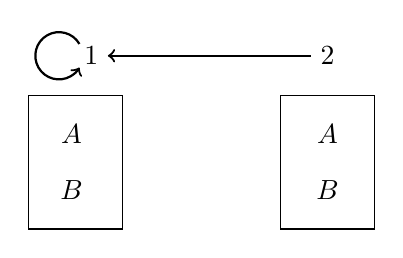
\begin{tikzpicture}
\node (atom1) at (0,1) {1};
\node (atom2) at (3,1) {2};
\node (atom3) at (-0.25,0) {$A$};
\node (atom4) at (3,0) {$\enot A$};
\node (atom5) at (-0.25,-0.7) {$\enot B$};
\node (atom6) at (3,-0.7) {$B$};
\draw[->, thick] (atom1)+(-0.15,0.15) arc (-330:-30:.3); 
%\draw[->, thick] (atom2)+(0.15,-0.15) arc (-150:150:.3); 
\draw[<-, thick] (atom1) -- (atom2);
\draw (-0.8,-1.2) rectangle (0.4,0.5);
\draw (2.4,-1.2) rectangle (3.6,0.5);
\end{tikzpicture}
\end{center}

\noindent Here is how to read the interpretation off from this diagram. It contains just two worlds, 1 and 2. The arrows between the worlds indicate the accessibility relation. So 1 and 2 both access 1, but neither 1 nor 2 accesses 2. The boxes at each world let us know which atomic sentences are true at each world: $A$ is true at 1 but false at 2; $B$ is false at 1 but true at 2. You may only write an atomic sentence or the negation of an atomic sentence into one of these boxes. We can figure out what truth-values the more complex sentences get at each world from that. For example, on this interpretation all of the following sentences are true at $w_1$:
\begin{itemize}
\item[]$A\eand\enot B$, $B\eif A$, $\Diamond A$, $\Box\enot B$
\end{itemize}
If you don't like thinking diagrammatically, then you can also present an interpretation like this:
\begin{itemize}
\item[$W$:]$1,2$
\item[$R$:]$\langle 1,1\rangle, \langle 2,1\rangle$
\item[]$\nu_{1}(A)=1, \nu_{2}(B)=0, \nu_{2}(A)=0, \nu_{2}(B)=1$
\end{itemize}
You will get the chance to cook up some interpretations of your own shortly, when we start looking at \emph{counter-interpretations}.

\section{A Semantics for System $K$}
\label{SemanticsK}

We can now extend all of the semantic concepts that you learnt in \emph{forall}$\meta{x}$ to cover ML:
\factoidbox{
\begin{itemize}
\item  $\meta{A}_1,\meta{A}_2, \dots \meta{A}_n\therefore\meta{C}$ is \textsc{modally valid} iff there is no world in any interpretation at which $\meta{A}_1,\meta{A}_2, \dots \meta{A}_n$ are all true and $\meta{C}$ is false.

\item $\meta{A}$ is a \textsc{modal logical truth} iff $\meta{A}$ is true at every world in every interpretation.

\item $\meta{A}$ is a \textsc{modal contradiction} iff $\meta{A}$ is false at every world in every interpretation.

\item $\meta{A}$ is \textsc{modally consistent} iff $\meta{A}$ is true at some world in some interpretation.
\end{itemize}
}
(From now on we will drop the explicit `modal' qualifications, since they can be taken as read.)

We can also extend our use of $\vDash$. However, we need to add subscripts again, just as we did with $\vdash$. So, when we want to say that $\meta{A}_1,\meta{A}_2, \dots \meta{A}_n\therefore\meta{C}$ is valid, we will write: $\meta{A}_1,\meta{A}_2, \dots \meta{A}_n\vDash_K\meta{C}$. Why did we choose the subscript $K$? Well, it turns out that there is an important relationship between system $K$ and the definition of validity we have just given. In particular, we have the following two results:
\begin{itemize}
\item If $\meta{A}_1,\meta{A}_2, \dots \meta{A}_n\vdash_K\meta{C}$, then $\meta{A}_1,\meta{A}_2, \dots \meta{A}_n\vDash_K\meta{C}$
\item If $\meta{A}_1,\meta{A}_2, \dots \meta{A}_n\vDash_K\meta{C}$, then $\meta{A}_1,\meta{A}_2, \dots \meta{A}_n\vdash_K\meta{C}$
\end{itemize}
The first result is known as a \emph{soundness} result, since it tells us that the rules of $K$ are good, sound rules: if you can vindicate an argument by giving a proof for it using system $K$, then that argument really is valid. The second result is known as a \emph{completeness} result, since it tells us that the rules of $K$ are broad enough to capture all of the valid arguments: if an argument is valid, then it will be possible to offer a proof in $K$ which vindicates it.

Now, it is one thing to state these results, quite another to prove them. However, I will not try to prove them here. If you are really interested, then you might want to look at any of the following: Garson's \emph{Modal Logic for Philosophers}; Priest's \emph{An Introduction to Non-Classical Logic}; Hughes and Cresswell's \emph{A New Introduction to Modal Logic}. None of these authors formulate their modal systems in quite the way we did, but it is not too hard hard to see how to translate their proofs of soundness and completeness over to our system. (The closest formulation is given by Garson, so the best place to start would be his \emph{Modal Logic for Philosophers}.)

For now, let's get more of a feel for this semantics by presenting some counter-interpretations. Consider the following (false) claim:
\begin{itemize}
\item[]
\begin{itemize}
\item[]$\enot A\vDash_K \enot \Diamond A$
\end{itemize}
\end{itemize}
In order to present a counter-interpretation to this claim, we need to cook up an interpretation which makes $\enot A$ true at some world $w$, and $\enot\Diamond A$ false at $w$. Here is one such interpretation, presented diagrammatically:
\begin{center}
\begin{tikzpicture}
\node (atom1) at (0,1) {1};
\node (atom2) at (3,1) {2};
\node (atom3) at (-0.25,0) {$\enot A$};
\node (atom4) at (3,0) {$A$};
\draw[->, thick] (atom1) -- (atom2);
\draw (-0.8,-0.6) rectangle (0.4,0.5);
\draw (2.4,-0.6) rectangle (3.6,0.5);
\end{tikzpicture}
\end{center}
It is easy to see that this will work as a counter-interpretation for our claim. First, $\enot A$ is true at world $1$. And second, $\enot\Diamond A$ is false at $1$: $A$ is true at $2$, and $2$ is accessible from $1$. So there is some world in this interpretation where $\enot A$ is true and $\enot\Diamond A$ is false, so it is not the case that $\enot A\vDash_K\enot\Diamond A$.


\section{A Semantics for System $T$}
\label{SemanticsT}

A few moments ago, I said that system $K$ is sound and complete. Where does that leave the other modal systems we looked at, namely $T$, $S4$ and $S5$? Well, they are all \emph{unsound}, relative to the definition of validity we gave above. For example, all of these systems allow us to infer $A$ from $\Box A$, even though $\Box A\nvDash_K A$.

Does that mean that these systems are a waste of time? Not at all! These systems are only unsound \emph{relative to the definition of validity we gave above}. (Or to use symbols, they are unsound relative to $\vDash_K$.) So when we are dealing with these stronger modal systems, we just need to modify our definition of validity to fit. This is where accessibility relations come in really handy.

When I introduced you to the idea of an accessibility relation, I said that it could be any relation between worlds that you like: you could have it relating every world to every world, no world to any world, or anything in between. That is how we were thinking of accessibility relations in our definition of $\vDash_K$. But if we wanted, we could start putting some restrictions on the accessibility relation. In particular, we might insist that it has to be \emph{reflexive}:
\begin{itemize}
\item $\forall wRww$
\end{itemize}
In English: every world accesses itself. Or in terms of relative possibility: every world is possible relative to itself. If we imposed this restriction, we could introduce a new consequence relation, $\vDash_T$, as follows:
\factoidbox{
$\meta{A}_1,\meta{A}_2, \dots \meta{A}_n\vDash_T \meta{C}$ iff there is no world in any interpretation \emph{which has a reflexive accessibility relation}, at which $\meta{A}_1,\meta{A}_2, \dots \meta{A}_n$ are all true and $\meta{C}$ is false
}
I have attached the $T$ subscript to $\vDash$ because it turns out that system $T$ is sound and complete relative to this new definition of validity:
\begin{itemize}
\item If $\meta{A}_1,\meta{A}_2, \dots \meta{A}_n\vdash_T\meta{C}$, then $\meta{A}_1,\meta{A}_2, \dots \meta{A}_n\vDash_T\meta{C}$
\item If $\meta{A}_1,\meta{A}_2, \dots \meta{A}_n\vDash_T\meta{C}$, then $\meta{A}_1,\meta{A}_2, \dots \meta{A}_n\vdash_T\meta{C}$
\end{itemize}
As before, I will not try to prove these soundness and completeness results. However, it is relatively easy to see how insisting that the accessibility relation must be reflexive will vindicate the $T$ rule:
\factoidbox{
\[\begin{nd}
\have[m]{m}{\Box \meta{A}}
\have[\, ]{n}{\meta{A}}\by{$T$}{m}
\end{nd}\]
}
To see this, just imagine trying to cook up a counter-interpretation to this claim:
\[
\Box \meta{A}\vDash_T \meta{A}
\]
We would need to construct a world, $w$, at which $\Box \meta{A}$ was true, but $\meta{A}$ was false. Now, if $\Box \meta{A}$ is true at $w$, then $\meta{A}$ must be true at every world $w$ accesses. But since the accessibility relation is reflexive, $w$ is accesses $w$. So $\meta{A}$ must be true at $w$. But now $\meta{A}$ must be true \emph{and} false at $w$. Contradiction!

\section{A Semantics for $S4$}
\label{SemanticsS4}

How else might we tweak our definition of validity? Well, we might also stipulate that the accessibility relation has to be \emph{transitive}:
\begin{itemize}
\item $\forall w_1\forall w_2\forall w_3 ((Rw_1w_2 \eand Rw_2w_3)\eif Rw_1w_3)$
\end{itemize}
In English: if $w_1$ accesses $w_2$, and $w_2$ accesses $w_3$, then $w_1$ accesses $w_3$. Or in terms of relative possibility: if $w_3$ is possible relative to $w_2$, and $w_2$ is possible relative to $w_1$, then $w_3$ is possible relative to $w_1$. If we added this restriction on our accessibility relation, we could introduce a new consequence relation, $\vDash_{S4}$, as follows:
\factoidbox{
$\meta{A}_1,\meta{A}_2, \dots \meta{A}_n\vDash_{S4} \meta{C}$ iff there is no world in any interpretation \emph{which has a reflexive and transitive accessibility relation}, at which $\meta{A}_1,\meta{A}_2, \dots \meta{A}_n$ are all true and $\meta{C}$ is false
}
I have attached the $S4$ subscript to $\vDash$ because it turns out that system $S4$ is sound and complete relative to this new definition of validity:
\begin{itemize}
\item If $\meta{A}_1,\meta{A}_2, \dots \meta{A}_n\vdash_{S4}\meta{C}$, then $\meta{A}_1,\meta{A}_2, \dots \meta{A}_n\vDash_{S4}\meta{C}$
\item If $\meta{A}_1,\meta{A}_2, \dots \meta{A}_n\vDash_{S4}\meta{C}$, then $\meta{A}_1,\meta{A}_2, \dots \meta{A}_n\vdash_{S4}\meta{C}$
\end{itemize}
As before, I will not try to prove these soundness and completeness results. However, it is relatively easy to see how insisting that the accessibility relation must be transitive will vindicate the $S4$ rule:
\factoidbox{
\[\begin{nd}
\have[m]{m}{\Box\meta{A}}
\have[\, ]{n}{\Box\Box\meta{A}}\by{$S4$}{m}
\end{nd}\]
}
To see this, just imagine trying to cook up a counter-interpretation to this claim:
\begin{itemize}
\item[]$\Box\meta{A} \vDash_{S4} \Box \Box \meta{A}$
\end{itemize}
We would need to construct a world, $w_1$, at which $\Box\meta{A}$ was true, but $\Box \Box \meta{A}$ was false. Now, if $\Box \Box \meta{A}$ is false at $w_1$, then $w_1$ must access some world, $w_2$, at which $\Box\meta{A}$ is false. Equally, if $\Box \meta{A}$ is false at $w_2$, then $w_2$ must access some world, $w_3$, at which $\meta{A}$ is false. We just said that $w_1$ accesses $w_2$, and $w_2$ accesses $w_3$. So since we are now insisting that the accessibility relation be transitive, $w_1$ must access $w_3$. And as $\Box\meta{A}$ is true at $w_1$, and $w_3$ is accessible from $w_1$, it follows that $\meta{A}$ must be true at $w_3$. So $\meta{A}$ is true \emph{and} false at $w_3$. Contradiction!

\section{A Semantics for $S5$}
\label{SemanticsS5}

Let's put one more restriction on the accessibility relation. This time, let's insist that it must be \emph{symmetric}:
\begin{itemize}
\item $\forall w_1\forall w_2(Rw_1w_2 \eif Rw_2w_1)$
\end{itemize}
In English: if $w_1$ accesses $w_2$, then $w_2$ accesses $w_1$. Or in terms of relative possibility: if $w_2$ is possible relative to $w_1$, then $w_1$ is possible relative to $w_2$. Logicians call a relation that is reflexive, symmetric and transitive an \emph{equivalence} relation. We can now define a new consequence relation, $\vDash_{S5}$, as follows:
\factoidbox{
$\meta{A}_1,\meta{A}_2, \dots \meta{A}_n\vDash_{S5} \meta{C}$ iff there is no world in any interpretation \emph{whose accessibility relation is an equivalence relation}, at which $\meta{A}_1,\meta{A}_2, \dots \meta{A}_n$ are all true and $\meta{C}$ is false
}
I have attached the $S5$ subscript to $\vDash$ because it turns out that system $S5$ is sound and complete relative to this new definition of validity:
\begin{itemize}
\item If $\meta{A}_1,\meta{A}_2, \dots \meta{A}_n\vdash_{S5}\meta{C}$, then $\meta{A}_1,\meta{A}_2, \dots \meta{A}_n\vDash_{S5}\meta{C}$
\item If $\meta{A}_1,\meta{A}_2, \dots \meta{A}_n\vDash_{S5}\meta{C}$, then $\meta{A}_1,\meta{A}_2, \dots \meta{A}_n\vdash_{S5}\meta{C}$
\end{itemize}
As ever, I will not try to prove these soundness and completeness results here. However, it is relatively easy to see how insisting that the accessibility relation must be an equivalence relation will vindicate the $S5$ rule:
\factoidbox{
\[\begin{nd}
\have[m]{m}{\Diamond \meta{A}}
\have[\, ]{n}{\Box\Diamond\meta{A}}\by{$S5$}{m}
\end{nd}\]
}
To see this, just imagine trying to cook up a counter-interpretation to this claim:
\[
\Diamond\meta{A} \vDash_{S5} \Box \Diamond \meta{A}
\]
We would need to construct a world, $w_1$, at which $\Diamond\meta{A}$ was true, but $\Box \Diamond \meta{A}$ was false. Now, if $\Diamond\meta{A}$ is true at $w_1$, then $w_1$ must access some world, $w_2$, at which $\meta{A}$ is true. Equally, if $\Box \Diamond \meta{A}$ is false at $w_1$, then $w_1$ must access some world, $w_3$, at which $\Diamond \meta{A}$ is false. Since we are now insisting that the accessibility relation is an equivalence relation, and hence symmetric, we can infer that $w_3$ accesses $w_1$. Thus, $w_3$ accesses $w_1$, and $w_1$ accesses $w_2$. Again, since we are now insisting that the accessibility relation is an equivalence relation, and hence transitive, we can infer that $w_3$ accesses $w_2$. But earlier we said that $\Diamond \meta{A}$ is false at $w_3$, which implies that $\meta{A}$ is false at every world which $w_3$ accesses. So $\meta{A}$ is true \emph{and} false at $w_2$. Contradiction!

In the definition of $\vDash_{S5}$, we stipulated that the accessibility relation must be an equivalence relation. But it turns out that there is another way of getting a notion of validity fit for $S5$. Rather than stipulating that the accessibility relation be an equivalence relation, we can instead stipulate that it be a \emph{universal} relation:
\begin{itemize}
\item $\forall w_1\forall w_2Rw_1w_2$
\end{itemize}
In English: every world accesses every world. Or in terms of relative possibility: every world is possible relative to every world. Using this restriction on the accessibility relation, we could have defined $\vDash_{S5}$ like this:
\factoidbox{
$\meta{A}_1,\meta{A}_2, \dots \meta{A}_n\vDash_{S5} \meta{C}$ iff there is no world in any interpretation \emph{which has a universal accessibility relation}, at which $\meta{A}_1,\meta{A}_2, \dots \meta{A}_n$ are all true and $\meta{C}$ is false
}
If we defined $\vDash_{S5}$ like this, we would still get the same soundness and completeness results for $S5$. What does this tell us? Well, it means that if we are dealing with a notion of necessity according to which \emph{every} world is possible relative to \emph{every} world, then we should use $S5$. What is more, most philosophers assume that the notions of necessity that they are most concerned with, like \emph{logical necessity} and \emph{metaphysical necessity}, are of exactly this kind. So $S5$ is the modal system that most philosophers use most of the time.

\practiceproblems

\problempart
Present counter-interpretations to the following false claims:
\begin{earg}
\item $\enot P \vDash_K \enot\Diamond P$
\item $\Box(P \eor Q)\vDash_K \Box P \eor \Box Q$
\item $\vDash_K \enot \Box (A\eand \enot A)$
\item $\Box A\vDash_K A$
\end{earg}

\problempart
Present counter-interpretations to the following false:
\begin{earg}
\item $\Diamond A\vDash_{S4} \Box\Diamond A$
\item $\Diamond A, \Box (\Diamond A \eif B)\vDash_{S4}\Box B$
\end{earg}

\problempart
Present counter-interpretations to the following false claims:
\begin{earg}
\item $\Box (M\eif O),\Diamond M\vDash_T O$
\item $\Box A\vDash_T \Box \Box A$
\end{earg}


\part{Advanced Topics}
\addtocontents{toc}{\protect\mbox{}\protect\hrulefill\par}

\chapter{Normal forms and expressive completeness}}\label{ch:normalform}

\section{Disjunctive Normal Form}\label{s:DNFDefined}

Say that a sentence is in \define{disjunctive normal form} \emph{iff} it meets all of the following conditions:
	\begin{earg}
		\item[(\textsc{dnf1})] No connectives occur in the sentence other than negations, conjunctions and disjunctions;
		\item[(\textsc{dnf2})] Every occurrence of negation has minimal scope (i.e.\ any `$\enot$' is immediately followed by an atomic sentence);
		\item[(\textsc{dnf3})] No disjunction occurs within the scope of any conjunction.
	\end{earg}
So, here are are some sentences in disjunctive normal form:
	\begin{center}
		$A$\\
		$(A \eand B) \eor (A \eand \enot B)$\\
		$(A \eand B) \eor (A \eand  B \eand C \eand \enot D \eand \enot E)$\\
		$A \eor (C \eand \enot P_{234} \eand P_{233} \eand Q) \eor \enot B$
	\end{center}
Note that I have here broken one of the maxims of this book (see \S\ref{s:InductionOnLength}) and \emph{temporarily} allowed myself to employ the relaxed bracketing-conventions that allow conjunctions and disjunctions to be of arbitrary length. These conventions make it easier to see when a sentence is in disjunctive normal form. I will continue to help myself to these relaxed conventions, without further comment.

To further illustrate the idea of disjunctive normal form, I will introduce some more notation. I write `$\pm\meta{A}$' to indicate that $\meta{A}$ is an atomic sentence which may or may not be prefaced with an occurrence of negation. Then a sentence in disjunctive normal form has the following shape:
	$$(\pm \meta{A}_1 \land \ldots \land \pm \meta{A}_i) \lor (\pm \meta{A}_{i+1} \land \ldots \land \pm\meta{A}_j) \lor \ldots \lor (\pm\meta{A}_{m+1} \land \ldots \land \pm \meta{A}_n)$$
We now know what it is for a sentence to be in disjunctive normal form. The result that we are aiming at is:
	\factoidbox{\label{thm:dnf}\textbf{Disjunctive Normal Form Theorem.} For any sentence, there is a tautologically equivalent sentence in disjunctive normal form.
	}
Henceforth, I will abbreviate `Disjunctive Normal Form' by `DNF'. 


\section{Proof of DNF Theorem via truth tables}\label{s:DNFTruthTable}
My first proof of the DNF Theorem employs truth tables. I will first illustrate the technique for finding an equivalent sentence in DNF, and then turn this illustration into a rigorous proof. 

Let's suppose we have some sentence, $\meta{S}$, which contains three atomic sentences, `$A$', `$B$' and `$C$'. The very first thing to do is fill out a complete truth table for $\meta{S}$. Maybe we end up with this:
\begin{center}
\begin{tabular}{c c c | c}
$A$ & $B$ & $C$ & $\meta{S}$\\
\hline
 T & T & T & T \\
 T & T & F & F \\
 T & F & T & T \\
 T & F & F & F \\
 F & T & T & F \\
 F & T & F & F \\
 F & F & T & T \\
 F & F & F & T
\end{tabular}
\end{center}
%Now, consider a sentence, whose only connectives are negations and conjunctions, where no connective occurs within the scope of any negation, e.g.:
%	$$A \eand \enot B \eand C$$
%This sentence is true when, and only when, `$A$' is true, `$B$' is false and `$C$' is true. Similarly, the sentence:
%	$$\enot A \eand \enot B \eand C$$
%this is true when, and only when, `$A$' is false, `$B$' is false and `$C$' is true. 
%
%A disjunction is true when, and only when, at least one of the disjuncts is true. So if I write down a disjunction of sentences of the above form, perhaps
%	$$(A \eand \enot B \eand C) \eor (\enot A \eand \enot B \eand C)$$
%then it will be true on exactly \emph{two} lines of the truth table which describes all possible valuations of `$A$', `$B$' and `$C$'. 
%
As it happens, $\meta{S}$ is true on four lines of its truth table, namely lines 1, 3, 7 and 8. Corresponding to each of those lines, I will write down four sentences, whose only connectives are negations and conjunctions, where every negation has minimal scope:
	\begin{earg}
		\item[\textbullet]  `$A \eand B \eand C$'\hfill which is true on line 1 (and only then)
		\item[\textbullet] `$A \eand \enot B \eand C$' \hfill which is true on line 3 (and only then)
		\item[\textbullet] `$\enot A \eand \enot B \eand C$' \hfill which is true on line 7 (and only then)
		\item[\textbullet] `$\enot A \eand \enot B \eand \enot C$' \hfill which is true on line 8 (and only then)
	\end{earg}
But if I now disjoin all of these conjunctions, like so:
$$(A \eand B \eand C) \eor (A \eand \enot B \eand C) \eor (\enot A \eand \enot B \eand C) \eor (\enot A \eand \enot B \eand \enot C)$$
I have a sentence in DNF which is true on exactly those lines where one of the disjuncts is true, i.e.\ it is true on (and only on) lines 1, 3, 7, and 8. So this sentence has exactly the same truth table as $\meta{S}$. So I have a sentence in DNF that is tautologically equivalent to $\meta{S}$. Which is exactly what I required!

Now, the strategy that I just adopted did not depend on the specifics of $\meta{S}$; it is perfectly general. Consequently, we can use it to obtain a simple proof of the DNF Theorem.

Pick any arbitrary sentence, $\meta{S}$, and let $\meta{A}_1, \ldots, \meta{A}_n$ be the atomic sentences that occur in $\meta{S}$. To obtain a sentence in DNF that is tautologically equivalent $\meta{S}$, we consider $\meta{S}$'s truth table. There are two cases to consider:
	\begin{enumerate}
		\item \emph{$\meta{S}$ is false on every line of its truth table.} Then, $\meta{S}$ is a contradiction. In that case, the contradiction $(\meta{A}_1 \eand \enot \meta{A}_1)$ is in DNF and tautologically equivalent to~$\meta{S}$. 
	
		\item \emph{$\meta{S}$ is true on at least one line of its truth table.}
		For each line $i$ of the truth table, let $\meta{B}_i$ be a conjunction of the form 
		$$(\pm\meta{A}_1 \land \ldots \land \pm\meta{A}_n)$$
		where the following rules determine whether or not to include a negation in front of each atomic sentence:
			\begin{align*}
				\meta{A}_m\text{ is a conjunct of }\meta{B}_i&\emph{ iff }\meta{A}_m\text{ is true on line }i\\
				\enot\meta{A}_m\text{ is a conjunct of }\meta{B}_i&\emph{ iff }\meta{A}_m\text{ is false on line }i
			\end{align*}
		Given these rules, a trivial proof by induction shows that $\meta{B_i}$ is true on (and only on) line $i$ of the truth table which considers all possible valuations of $\meta{A}_1, \ldots, \meta{A}_n$ (i.e.\ $\meta{S}$'s truth table). 
		
		Next, let $i_1, i_2, \ldots, i_m$ be the numbers of the lines of the truth table where $\meta{S}$ is \emph{true}. Now let $\meta{D}$ be the sentence:
		$$\meta{B}_{i_1} \eor \meta{B}_{i_2} \eor \ldots \eor \meta{B}_{i_m}$$
		Since $\meta{S}$ is true on at least one line of its truth table, $\meta{D}$ is indeed well-defined; and in the limiting case where $\meta{S}$ is true on exactly one line of its truth table, $\meta{D}$ is just $\meta{B}_{i_1}$, for some $i_1$.
		
		By construction, $\meta{D}$ is in DNF. Moreover, by construction, for each line $i$ of the truth table: $\meta{S}$ is true on line $i$ of the truth table \emph{iff} one of $\meta{D}$'s disjuncts (namely, $\meta{B_i}$) is true on, and only on, line $i$. (Again, this is shown by a trivial proof by induction.) Hence $\meta{S}$ and $\meta{D}$ have the same truth table, and so are tautologically equivalent.
	\end{enumerate}
	These two cases are exhaustive and, either way, we have a sentence in DNF that is tautologically equivalent to $\meta{S}$.

So we have proved the DNF Theorem. Before I say any more, though, I should immediately flag that I am hereby returning to the austere definition of a (TFL) sentence, according to which we can assume that any conjunction has exactly two conjuncts, and any disjunction has exactly two disjuncts.


\section{Conjunctive Normal Form}\label{s:CNF}
So far in this chapter, I have discussed \emph{disjunctive} normal form. Given the duality of disjunction and conjunction (see \S\ref{s:Duality}), it may not come as a surprise to hear that there is also such a thing as \emph{conjunctive normal form} (CNF).

The definition of CNF is exactly analogous to the definition of DNF. So, a sentence is in CNF \emph{iff} it meets all of the following conditions:
	\begin{earg}
		\item[(\textsc{cnf1})] No connectives occur in the sentence other than negations, conjunctions and disjunctions;
		\item[(\textsc{cnf2})] Every occurrence of negation has minimal scope;
		\item[(\textsc{cnf3})] No conjunction occurs within the scope of any disjunction. 
	\end{earg}
Generally, then, a sentence in CNF looks like this
	$$(\pm \meta{A}_1 \lor \ldots \lor \pm \meta{A}_i) \land (\pm \meta{A}_{i+1} \lor \ldots \lor \pm\meta{A}_j) \land \ldots \land (\pm\meta{A}_{m+1} \lor\ldots \lor \pm \meta{A}_n)$$
where each $\meta{A}_k$ is an atomic sentence.

Since `$\enot$' is its own dual, and `$\eor$' and `$\eand$' are the duals of each other, it is immediate clear that if a sentence is in DNF, then its dual is in CNF; and \emph{vice versa}. Armed with this insight, we can immediately prove another normal form theorem:
	\factoidbox{\label{thm:cnf}\textbf{Conjunctive Normal Form Theorem.} For any sentence, there is a tautologically equivalent sentence in conjunctive normal form.}

        
	Given a TFL sentence, $\meta{S}$, we begin by writing down the complete truth table for $\meta{S}$.
	
	If $\meta{S}$ is \emph{true} on every line of the truth table, then $\meta{S}$ and $(\meta{A}_1 \eor \enot \meta{A}_1)$ are tautologically equivalent.
	
	If $\meta{S}$ is \emph{false} on at least one line of the truth table then, for every line on the truth table where $\meta{S}$ is false, write down a disjunction $(\pm\meta{A}_1 \eor \ldots \eor \pm\meta{A}_n)$ which is \emph{false} on (and only on) that line. Let $\meta{C}$ be the conjunction of all of these disjuncts; by construction, $\meta{C}$ is in CNF and $\meta{S}$ and $\meta{C}$ are tautologically equivalent.

\practiceproblems
\problempart
\label{pr.DNF}
Consider the following sentences:
	\begin{earg}
		\item $(A \eif \enot B)$
		\item $\enot (A \eiff B)$
		\item $(\enot A \eor \enot (A \eand B))$
		\item $(\enot (A \eif B ) \eand (A \eif C))$
		\item $(\enot (A \eor B) \eiff ((\enot C \eand \enot A) \eif \enot B))$
		\item $((\enot (A \eand \enot B) \eif C) \eand \enot (A \eand D))$
	\end{earg}
        For each sentence, find a tautologically equivalnet sentence in DNF and one in CNF.
        
\section{The expressive adequacy of TFL}
In discussing duality (\S\ref{s:Duality}), I introduced the general idea of an $n$-place connective. We might, for example, define a three-place connective, `$\heartsuit$', into existence, by stipulating that it is to have the following characteristic truth table:
\begin{center}
\begin{tabular}{c c c | c}
$\meta{A}$ & $\meta{B}$ & $\meta{C}$ & $\heartsuit(\meta{A},\meta{B},\meta{C})$\\
\hline
 T & T & T & F \\
 T & T & F & T \\
 T & F & T & T \\
 T & F & F & F \\
 F & T & T & F \\
 F & T & F & T \\
 F & F & T & F \\
 F & F & F & F
\end{tabular}
\end{center}
Probably this new connective would not correspond with any natural English expression (in the way that `$\eand$' corresponds with `and'). But a question arises: if we wanted to employ a connective with this characteristic truth table, must we add a \emph{new} connective to TFL? Or can we get by with the connectives we \emph{already have}?

Let us make this question more precise. Say that some connectives are \define{jointly expressively adequate} \emph{iff}, for any possible truth function, there is a scheme containing only those connectives which expresses that truth function. Since we can represent truth functions using characteristic truth tables, we could equivalently say the following: some connectives are jointly expressively adequate \emph{iff}, for any possible truth table, there is a scheme containing only those connectives with that truth table.

I say `scheme' rather than `sentence', because we are not concerned with something as specific as a sentence. To see why, consider the characteristic truth table for conjunction; this schematically encodes the information that a conjunction $(\meta{A} \eand \meta{B})$ is true iff both $\meta{A}$ and $\meta{B}$ are true (whatever $\meta{A}$ and $\meta{B}$ might be). When we discuss expressive adequacy, we are considering something at the same level of generality. 

The general point is, when we are armed with some jointly expressively adequate connectives, no truth function lies beyond our grasp. And in fact, we are in luck.
	\factoidbox{\label{thm:ExpressiveAdequacy}\textbf{Expressive Adequacy Theorem.}
		The connectives of TFL are jointly expressively adequate. Indeed, the following pairs of connectives are jointly expressively adequate:
			\begin{earg}
				\item\label{expressive:eor} `$\enot$' and `$\eor$'
				\item\label{expressive:eand} `$\enot$' and `$\eand$'
				\item\label{expressive:eif} `$\enot$' and `$\eif$'
			\end{earg}}

	 Given any truth table, we can use the method of proving the DNF Theorem (or the CNF Theorem) via truth tables, to write down a scheme which has the same truth table. For example, employing the truth table method for proving the DNF Theorem, I can tell you that the following scheme has the same characteristic truth table as $\heartsuit(\meta{A},\meta{B},\meta{C})$, above:
		$$(\meta{A} \eand \meta{B} \eand \enot \meta{C}) \eor (\meta{A} \eand \enot\meta{B} \eand \meta{C}) \eor (\enot \meta{A} \eand \meta{B} \eand \enot \meta{C})$$			
			It follows that the connectives of TFL are jointly expressively adequate. I now prove each of the subsidiary results.
	
				\emph{Subsidiary Result \ref{expressive:eor}: expressive adequacy of `$\enot$' and `$\eor$'.} Observe that the scheme that we generate, using the truth table method of proving the DNF Theorem, will only contain the connectives `$\enot$', `$\eand$' and `$\eor$'. So it suffices to show that there is an equivalent scheme which contains only `$\enot$' and `$\eor$'. To show do this, we simply consider that
		\begin{align*}
		(\meta{A} \eand \meta{B}) & \text{\quad and \quad} \enot(\enot \meta{A} \eor\enot \meta{B})
		\end{align*}
		are tautologically equivalent.

		\emph{Subsidiary Result \ref{expressive:eand}: expressive adequacy of `$\enot$' and `$\eand$'.} Exactly as in Subsidiary Result \ref{expressive:eor}, making use of the fact that
		\begin{align*}
		(\meta{A} \eor \meta{B}) & \text{\quad and \quad}\enot(\enot \meta{A} \eand\enot \meta{B})
		\end{align*}
                are tautologically equivalent.

			\emph{Subsidiary Result \ref{expressive:eif}: expressive adequacy of `$\enot$' and `$\eif$'.} 		Exactly as in Subsidiary Result \ref{expressive:eor}, making use of these equivalences instead:
		\begin{align*}
		(\meta{A} \eor \meta{B}) &\text{\quad and \quad} (\enot \meta{A} \eif\meta{B})\\
		(\meta{A} \eand \meta{B}) &\text{\quad and \quad} \enot(\meta{A} \eif \enot\meta{B})
		\end{align*}
		Alternatively, we could simply rely upon one of the other two subsidiary results, and (repeatedly) invoke only one of these two equivalences.

In short, there is never any \emph{need} to add new connectives to TFL. Indeed, there is already some redundancy among the connectives we have: we could have made do with just two connectives, if we had been feeling really austere.

\section{Individually expressively adequate connectives}
In fact, some two-place connectives are \emph{individually} expressively adequate. These connectives are not standardly included in TFL, since they are rather cumbersome to use. But their existence shows that, if we had wanted to, we could have defined a truth-functional language that was expressively adequate, which contained only a single primitive connective.

The first such connective we will consider is `$\uparrow$', which has the following characteristic truth table. 
\begin{center}
\begin{tabular}{c c | c}
$\meta{A}$ & $\meta{B}$ & $\meta{A} \mathrel{\uparrow} \meta{B}$\\
\hline
 T & T & F \\
 T & F & T \\
 F & T & T  \\
 F & F & T
\end{tabular}
\end{center}
 This is often called `the Sheffer stroke', after Henry Sheffer, who used it to show how to reduce the number of logical connectives in Russell and Whitehead's \emph{Principia Mathematica}.\footnote{Sheffer, `A Set of Five Independent Postulates for Boolean Algebras, with application to logical constants,' (1913, \emph{Transactions of the American Mathematical Society} 14.4)} (In fact, Charles Sanders Peirce had anticipated Sheffer by about 30 years, but never published his results.)\footnote{See Peirce, `A Boolian Algebra with One Constant', which dates to c.1880; and Peirce's \emph{Collected Papers}, 4.264--5.} It is quite common, as well, to call it `nand', since its characteristic truth table is the negation of the truth table for `$\eand$'.
\factoidbox{\label{prop:upexpressive}`$\uparrow$' is expressively adequate all by itself.}

		Theorem \ref{thm:ExpressiveAdequacy} tells us that `$\enot$' and `$\eor$' are jointly expressively adequate. So it suffices to show that, given any scheme which contains only those two connectives, we can rewrite it as a tautologically equivalent scheme which contains only `$\uparrow$'. As in the proof of the subsidiary cases of Theorem \ref{thm:ExpressiveAdequacy}, then, we simply apply the following equivalences:
		\begin{align*}
			\enot \meta{A} &\text{\quad and \quad} (\meta{A} \uparrow \meta{A})\\
			(\meta{A} \eor \meta{B}) & \text{\quad and \quad} ((\meta{A} \uparrow \meta{A}) \uparrow (\meta{B} \uparrow \meta{B}))
		\end{align*}
		 to Subsidiary Result \ref{expressive:eor} of Theorem \ref{thm:ExpressiveAdequacy}.

Similarly, we can consider the connective `$\downarrow$':
\begin{center}
\begin{tabular}{c c | c}
$\meta{A}$ & $\meta{B}$ & $\meta{A} \mathrel{\downarrow} \meta{B}$\\
\hline
 T & T & F \\
 T & F & F  \\
 F & T & F  \\
 F & F & T
\end{tabular}
\end{center}
This is sometimes called the `Peirce arrow' (Peirce himself called it `ampheck'). More often, though, it is called `nor', since its characteristic truth table is the negation of `$\eor$'.
	\factoidbox{
	`$\downarrow$' is expressively adequate all by itself. }


	As in Proposition \ref{prop:upexpressive}, although invoking the dual equivalences:
		\begin{align*}
			\enot \meta{A} &\text{\quad and \quad} (\meta{A} \downarrow \meta{A})\\
			(\meta{A} \eand \meta{B}) & \text{\quad and \quad} ((\meta{A} \downarrow \meta{A}) \downarrow (\meta{B} \downarrow \meta{B}))
		\end{align*}
		and Subsidiary Result \ref{expressive:eand} of Theorem \ref{thm:ExpressiveAdequacy}.


\section{Failures of expressive adequacy}
 In fact, the \emph{only} two-place connectives which are individually expressively adequate are `$\uparrow$' and `$\downarrow$'. But how would we show this? More generally, how can we show that some connectives are \emph{not} jointly expressively adequate? 
 
The obvious thing to do is to try to find some truth table which we \emph{cannot} express, using just the given connectives. But there is a bit of an art to this. Moreover, in the end, we will have to rely upon induction; for we will need to show that \emph{no} scheme -- no matter how \emph{long} -- is capable of expressing the target truth table. 
 
 To make this concrete, let's consider the question of whether `$\eor$' is expressively adequate all by itself. After a little reflection, it should be clear that it is not. In particular, it should be clear that any scheme which only contains disjunctions cannot have the same truth table as negation, i.e.:
				\begin{center}
				\begin{tabular}{c | c}
				$\meta{A}$ & $\enot \meta{A}$\\
				\hline
				 T &  F \\
				 F & T
				\end{tabular}
				\end{center}
The intuitive reason, why this should be so, is simple: the top line of the desired truth table needs to have the value False; but the top line of any truth table for a scheme which \emph{only} contains disjunctions will always be True.
 	\factoidbox{
		`$\eor$' is not expressively adequate by itself.}

        In fact, we can generalise this to:
        
	\factoidbox{The \emph{only} two-place connectives that are expressively adequate by themselves are `$\uparrow$' and `$\downarrow$'. }

\factoidbox{\label{prop:Eiff4}
  Exactly four 2-place truth functions can be expressed using schemes whose only connectives are biconditionals:
			\begin{align*}
				\meta{A} \eiff \meta{A}\\
				\meta{A}\\
				\meta{B}\\
				\meta{A} \eiff \meta{B}
			\end{align*}
			It is clear that we can express all four, and that they are distinct.}
		




\appendix
\part*{Appendices}
\addcontentsline{toc}{part}{Appendices}
\addtocontents{toc}{\protect\mbox{}\protect\hrulefill\par}

\input{forallx-yyc-notation} % RZ for some reason, with an \include here the TOC gets messed up
%!TEX root = forallxyyc.tex

\chapter{Alternative proof systems}
In formulating our natural deduction system, we treated certain rules of natural deduction as \emph{basic}, and others as \emph{derived}. However, we could equally well have taken various different rules as basic or derived. We will illustrate this point by considering some alternative treatments of disjunction, negation, and the quantifiers. We will also explain why we have made the choices that we have.


\section{Alternative disjunction elimination}
Some systems take DS as their basic rule for disjunction elimination. Such systems can then treat the $\eor$E rule as a derived rule. For they might offer the following proof scheme: 
\begin{fitchproof}
  \have[m]{ab}{\metav{A}\eor\metav{B}}
  \open
    \hypo[i]{a}{\metav{A}} {}
    \have[j]{c1}{\metav{C}}
  \close
  \open
    \hypo[k]{b}{\metav{B}}{}
    \have[l]{c2}{\metav{C}}
  \close
  \have[n]{aic}{\metav{A} \eif \metav{C}}\ci{a-c1}
  \have{bic}{\metav{B} \eif \metav{C}}\ci{b-c2}
  \open
    \hypo{nc}{\enot\metav{C}}
    \open
      \hypo{a2}{\metav{A}}
      \have{c3}{\metav{C}}\ce{a2,aic}
      \have{bot1}{\ered}\ne{nc,c3}
    \close
    \have{na}{\enot\metav{A}}\ni{a2-bot1}
    \have{b2}{\metav{B}}\ds{ab,na}
    \have{c4}{\metav{C}}\ce{b2,bic}
    \have{bot2}{\ered}\ne{nc,c4}
  \close
  \have{con}{\metav{C}}\ip{nc-bot2}
\end{fitchproof}
So why did we choose to take $\eor$E as basic, rather than DS?\footnote{P.D.\ Magnus's original version of this book went the other way.} Our reasoning is that DS involves the use of `$\enot$' in the statement of the rule. It is in some sense `cleaner' for our disjunction elimination rule to avoid mentioning \emph{other} connectives. 


\section{Alternative negation rules}
Some systems take the following rule as their basic negation introduction rule:
\begin{fitchproof}
	\open
		\hypo[m]{a}{\metav{A}}
		\have[n-1]{b}{\metav{B}}
		\have[n]{nb}{\enot\metav{B}}
	\close
	\have[\ ]{}{\enot\metav{A}}\by{$\enot$I*}{a-nb}
\end{fitchproof}
and a corresponding version of the rule we called IP as their basic negation elimination rule:
\begin{fitchproof}
	\open
		\hypo[m]{na}{\enot\metav{A}}
		\have[n][-1]{b}{\metav{B}}
		\have{nb}{\enot\metav{B}}
	\close
	\have[\ ]{a}{\metav{A}}\by{$\enot$E*}{na-nb}
\end{fitchproof}
Using these two rules, we could we could have avoided all use of the symbol `$\ered$' altogether.\footnote{Again, P.D.\ Magnus's original version of this book went the other way.} The resulting system would have had fewer rules than ours.

Another way to deal with negation is to use either LEM or DNE as a basic rule and introduce IP as a derived rule. Typically, in such a system the rules are given different names, too. E.g., sometimes what we call $\enot$E is called $\ered$I, and what we call X is called $\ered$E.\footnote{The version of this book due to Tim Button goes this route and replaces IP with LEM, which he calls TND, for ``tertium non datur.''}

So why did we chose our rules for negation and contradiction? 

Our first reason is that adding the symbol `$\ered$' to our natural deduction system makes proofs considerably easier to work with. For instance, in our system it's always clear what the conclusion of a subproof is: the sentence on the last line, e.g.\ $\ered$ in IP or $\enot$I. In $\enot$I* and $\enot$E*, subproofs have two conclusions, so you can't check at one glance if an application of them is correct. 

Our second reason is that a lot of fascinating philosophical discussion has focussed on the acceptability or otherwise of indirect proof IP (equivalently, excluded middle, i.e.\ LEM, or double negation elimination DNE) and explosion (i.e.\ X). By treating these as separate rules in the proof system, you will be  in a better position to engage with that philosophical discussion. In particular: having invoked these rules explicitly, it would be much easier for us to know what a system which lacked these rules would look like.

This discussion, and in fact the vast majority of mathematical study on applications of natural deduction proofs beyond introductory courses, makes reference to a different version of natural deduction. This version was invented by Gerhard Gentzen in 1935 as refined by Dag Prawitz in 1965. Our set of basic rules coincides with theirs. In other words, the rules we use are those that are standard in philosophical and mathematical discussion of natural deduction proofs outside of introductory courses.



\section{Alternative quantification rules}
An alternative approach to the quantifiers is to take as basic the rules for $\forall$I and $\forall$E from \S\ref{s:BasicFOL}, and also two CQ rule which allow us to move from $\forall \metav{x} \enot \metav{A}$ to $\enot \exists \metav{x} \metav{A}$ and vice versa.\footnote{Warren Goldfarb follows this line in \emph{Deductive Logic}, 2003, Hackett Publishing Co.}  

Taking only these rules as basic, we could have derived the  $\exists$I and $\exists$E rules provided in \S\ref{s:BasicFOL}. To derive the $\exists$I rule is fairly simple. Suppose $\metav{A}$ contains the name $\metav{c}$, and contains no instances of the variable $\metav{x}$, and that we want to do the following:
\begin{fitchproof}
	\have[m]{a}{\metav{A}(\ldots \metav{c} \ldots \metav{c}\ldots)}
	\have[k]{c}{\exists \metav{x} \metav{A}(\ldots \metav{x} \ldots \metav{c}\ldots)}
\end{fitchproof}
This is not yet permitted, since in this new system, we do not have the $\exists$I rule. We can, however, offer the following:
\begin{fitchproof}
	\hypo[m]{a}{\metav{A}(\ldots \metav{c} \ldots \metav{c}\ldots)}
	\open
		\hypo{nEna}{\enot \exists \metav{x} \metav{A}(\ldots \metav{x} \ldots \metav{c}\ldots)}
		\have{Ana}{\forall \metav{x} \enot \metav{A}(\ldots \metav{x} \ldots \metav{c}\ldots)}\cq{nEna}
		\have{nAc}{\enot\metav{A}(\ldots \metav{c} \ldots \metav{c}\ldots)}\Ae{Ana}
		\have{red}{\ered}\ne{nAc, a}
	\close
	\have{nnEa}{\exists \metav{x} \metav{A}(\ldots \metav{x} \ldots \metav{c}\ldots)}\ip{nEna-red}
\end{fitchproof}\noindent
To derive the $\exists$E rule is rather more subtle. This is because the $\exists$E rule has an important constraint (as, indeed, does the $\forall$I rule), and we need to make sure that we are respecting it. So, suppose we are in a situation where we \emph{want} to do the following:
\begin{fitchproof}
	\have[m]{ExA}{\exists \metav{x} \metav{A}(\ldots \metav{x} \ldots \metav{x}\ldots)}
	\open
		\hypo[i]{Ac}{\metav{A}(\ldots \metav{c} \ldots \metav{c}\ldots)}
		\have[j]{B}{\metav{B}}
	\close
	\have[k]{end}{\metav{B}}
\end{fitchproof}\noindent
 where $\metav{c}$ does not occur in any undischarged assumptions, or in $\metav{B}$, or in $\exists \metav{x} \metav{A}(\ldots \metav{x} \ldots \metav{x}\ldots)$. Ordinarily, we would be allowed to use the $\exists$E rule; but we are not here assuming that we have access to this rule as a basic rule. Nevertheless, we could offer the following, more complicated derivation:
 
\begin{fitchproof}
	\have[m]{ExA}{\exists \metav{x} \metav{A}(\ldots \metav{x} \ldots \metav{x}\ldots)}
	\open
		\hypo[i]{Ac}{\metav{A}(\ldots \metav{c} \ldots \metav{c}\ldots)}
		\have[j]{B}{\metav{B}}
	\close
	\have[k]{condi}{\metav{A}(\ldots \metav{c} \ldots \metav{c}\ldots) \eif \metav{B}}\ci{Ac-B}
	\open
		\hypo{nB}{\enot \metav{B}}
		\have{nAc}{\enot \metav{A}(\ldots \metav{c} \ldots \metav{c}\ldots)}\mt{condi, nB}
		\have{AxnA}{\forall \metav{x} \enot \metav{A}(\ldots \metav{x} \ldots \metav{x}\ldots)}\Ai{nAc}
		\have{nEA}{\enot \exists \metav{x} \metav{A}(\ldots \metav{x} \ldots \metav{x}\ldots)}\cq{AxnA}
		\have{red2}{\ered}\ne{nEA, ExA}
	\close
	\have{nnB}{\metav{B}}\ip{nB-red2}
\end{fitchproof}\noindent
We are permitted to use $\forall$I on line $k+3$ because $\metav{c}$ does not occur in any  undischarged assumptions or in $\metav{B}$. The entries on lines $k+4$ and $k+1$ contradict each other, because $\metav{c}$ does not occur in $\exists \metav{x} \metav{A}(\ldots \metav{x} \ldots \metav{x} \ldots)$.

Armed with these derived rules, we could now go on to derive the two remaining CQ rules, exactly as in \S\ref{s:DerivedFOL}.

So, why did we start with all of the quantifier rules as basic, and then derive the CQ rules? 

Our first reason is that it seems more intuitive to treat the quantifiers as on a par with one another, giving them their own basic rules for introduction and elimination. 

Our second reason relates to the discussion of alternative negation rules. In the derivations of the rules of $\exists$I and $\exists$E that we have offered in this section, we invoked~IP.  But, as we mentioned earlier, IP is a contentious rule. So, if we want to move to a system which abandons IP, but which still allows us to use existential quantifiers, we will want to take the introduction and elimination rules for the quantifiers as basic, and take the CQ rules as derived. (Indeed, in a system without IP, LEM, and DNE, we will be \emph{unable} to derive the CQ rule which moves from $\enot \forall \metav{x} \metav{A}$ to $\exists \metav{x} \enot \metav{A}$.)

\include{forallx-yyc-quickreference}

\backmatter

\glsaddall
\addtocontents{toc}{\protect\mbox{}\protect\hrulefill\par}
\printglossaries
\include{forallx-yyc-backmatter}

